% Copyright (c) 2025 Carl Martin Ludvig Sinander.

% This program is free software: you can redistribute it and/or modify
% it under the terms of the GNU General Public License as published by
% the Free Software Foundation, either version 3 of the License, or
% (at your option) any later version.

% This program is distributed in the hope that it will be useful,
% but WITHOUT ANY WARRANTY; without even the implied warranty of
% MERCHANTABILITY or FITNESS FOR A PARTICULAR PURPOSE. See the
% GNU General Public License for more details.

% You should have received a copy of the GNU General Public License
% along with this program. If not, see <https://www.gnu.org/licenses/>.

%                                   _     _
%    _ __  _ __ ___  __ _ _ __ ___ | |__ | | ___
%   | '_ \| '__/ _ \/ _` | '_ ` _ \| '_ \| |/ _ \
%   | |_) | | |  __/ (_| | | | | | | |_) | |  __/
%   | .__/|_|  \___|\__,_|_| |_| |_|_.__/|_|\___|
%   |_|


%%% bug catcher
\RequirePackage[l2tabu,orthodox]{nag}

%%% document class
\documentclass[11pt,letterpaper,reqno,oneside]{book}

%%% settings
\input{preamble.tex}

%%% for \widthof
\usepackage{calc}

% break DOIs in bibliography
\setcounter{biburlnumpenalty}{100}

% raise hypertargets above baseline
\makeatletter
	\newcommand{\hyperdest}[1]{\Hy@raisedlink{\hypertarget{#1}{}}}
\makeatother

% % watermark on every page (for version control)
% \usepackage[anchor=ll,pos={0.1cm,0.5cm},fontsize=0.2cm,angle=0,alignment=l]{draftwatermark}
% \SetWatermarkText{\normalfont\hspace{0.37em}version:\\\normalfont {\datestyle\today}\\\normalfont\hspace{0.37em}at {\currenttime}}


%%% bibliography
\addbibresource{bibl.bib}


%______________________________________________________________________________




%    _____ _ _   _
%   |_   _(_) |_| | ___
%     | | | | __| |/ _ \
%     | | | | |_| |  __/
%     |_| |_|\__|_|\___|


\title{\scshape Advanced game theory}

\author{Ludvig Sinander \\
University of Oxford}

\date{\small This version: 15 December 2025}

% \date{\emph{version:} {\datestyle\today} at {\currenttime} \\ \hspace{0pt} \\ \hspace{0pt} \\ \bfseries please report typos!}

\makeatletter
	\AtBeginDocument{ \hypersetup{
		pdftitle = {Advanced game theory},
		pdfauthor = {Ludvig Sinander}
		} }
\makeatother



%______________________________________________________________________________




%    ____                                        _
%   |  _ \  ___   ___ _   _ _ __ ___   ___ _ __ | |_
%   | | | |/ _ \ / __| | | | '_ ` _ \ / _ \ '_ \| __|
%   | |_| | (_) | (__| |_| | | | | | |  __/ | | | |_
%   |____/ \___/ \___|\__,_|_| |_| |_|\___|_| |_|\__|


\begin{document}

\maketitle

\pagebreak
\hspace{1pt}\vfill
\noindent
Copyright \copyright{} 2025 Carl Martin Ludvig Sinander.

\begin{quotation}
\noindent
Permission is granted to copy, distribute and/or modify this document under the terms of the \href{https://www.gnu.org/licenses/fdl}{GNU Free Documentation License}, Version 1.3 or any later version published by the Free Software Foundation; with no Invariant Sections, no Front-Cover Texts, and no Back-Cover Texts. A copy of the license is included in the section entitled `GNU
Free Documentation License'.
\end{quotation}

\noindent
This is a `copyleft' licence.
Visit \href{https://www.gnu.org/licenses/copyleft}{gnu.org/licenses/copyleft} to learn more.



%%%%%%%%%%%%%%%%%%%%%%
%%%%%%%%%%%%%%%%%%%%%%
%%%%%%%%%%%%%%%%%%%%%%
\chapter*{Preface}
\label{preface}
%%%%%%%%%%%%%%%%%%%%%%
%%%%%%%%%%%%%%%%%%%%%%
%%%%%%%%%%%%%%%%%%%%%%

These are the notes for the game theory component of the first-year graduate microeconomics sequence at Oxford, which I first taught in winter 2025.
Thanks to Sami Petersen for exceptionally perceptive proofreading, and to Matteo Escudé, Alexis Ghersengorin, Vishnu Gorthi, Sanjari Kalantri, Malayvardhan Prajapati, Augustus Smith, Alex Teytelboym, Runhuan Wang and Sally Yang for comments.



%%%%%%%%%%%%%%%%%%%
%%%%%%%%%%%%%%%%%%%
% Table of contents
\pagebreak
\microtypesetup{protrusion=false}
\setcounter{tocdepth}{1}
\tableofcontents
\microtypesetup{protrusion=true}
%%%%%%%%%%%%%%%%%%%
%%%%%%%%%%%%%%%%%%%



\setcounter{chapter}{-1}
%%%%%%%%%%%%%%%%%%%%%%
%%%%%%%%%%%%%%%%%%%%%%
%%%%%%%%%%%%%%%%%%%%%%
\chapter{Introduction}
\label{ch0}
%%%%%%%%%%%%%%%%%%%%%%
%%%%%%%%%%%%%%%%%%%%%%
%%%%%%%%%%%%%%%%%%%%%%

These notes cover a number of topics in game theory which are standard and important, but typically not covered in undergraduate courses. These are dominance and rationalisability (including Pearce's lemma), Tarski's fixed-point theorem, comparative statics, games of strategic complements, the one-shot deviation principle, and the APS \parencite{AbreuPearceStacchetti1990} technique.

The mathematical prerequisites are relatively slight: some basic real analysis (limits, continuity, integrals) is presumed, as well as the separating hyperplane theorem. Some useful mathematical background is reviewed in \cref{math}.

The notes also assume a working knowledge of basic topics in game theory, including normal-form games, incomplete-information/Bayesian games, and extensive-form games, and the basic solution concepts for these: Nash equilibrium, Bayes--Nash equilibrium, backward induction, subgame-perfect (Nash) equilibrium, and (some version of) perfect Bayesian equilibrium and/or sequential equilibrium. We now tersely recap these. For more, consult one of the classics \parencite{OsborneRubinstein1994,FudenbergTirole1991book,Myerson1991}, or try out a textbook from the new generation \parencite{MaschlerSolanZamir2020,Kreps2023,BattigalliCatoniniDevito2024}.



%%%%%%%%%%%%%%%%%%%%%%%%%%%%%%%%%%%
%%%%%%%%%%%%%%%%%%%%%%%%%%%%%%%%%%%
\section{Recap: normal-form games}
\label{ch0:normal}
%%%%%%%%%%%%%%%%%%%%%%%%%%%%%%%%%%%
%%%%%%%%%%%%%%%%%%%%%%%%%%%%%%%%%%%

A normal-form game is a formalism for describing a strategic situation in which players take actions in ignorance of which actions the other players have chosen; that is, moves are (epistemologically) simultaneous, not sequential.

A \emph{normal-form game} (also called a `strategic-form game') is a triplet $\left( I, (A_i, u_i)_{i \in I} \right)$, where $I$ is a non-empty set, and for each $j \in I$, $A_j$ is a non-empty set and $u_j$ is a function $\prod_{i \in I} A_i \to \R$.%
	\footnote{See \cref{math:set} for a review of (Cartesian) product sets.}
The interpretation is that $I$ is the set of players, that each player $j \in I$ has a set $A_j$ of actions available to her, and that her payoff is $u_j(a)$ if actions $a=(a_i)_{i \in I} \in \prod_{i \in I} A_i$ are played. The game is called \emph{finite} iff the player set $I$ and action sets $A_i$ (for each $i \in I$) are finite.%
	\footnote{A technicality: in case the game is \emph{not} finite, it is often necessary to augment the triplet $\left( I, (A_i, u_i)_{i \in I} \right)$ with measurable structure.}

In case the game is finite and has only $\abs*{I}=2$ players, it may be represented by a \emph{payoff matrix:} enumerate player~1's actions as $A_1 \equiv \{a_1,\dots,a_{\abs*{A_1}}\}$ and player~2's as $A_2 \equiv \{b_1,\dots,b_{\abs*{A_2}}\}$, and summarise $u_1$ and $u_2$ by the $\abs*{A_1} \times \abs*{A_2}$ matrix whose $(k,\ell)$ entry is $\left( u_1\left( a_k, b_\ell \right), u_2\left( a_k, b_\ell \right) \right)$.

We write $A \coloneqq \prod_{i \in I} A_i$ for the set of \emph{action profiles.} For any action profile $a = (a_i)_{i \in I}$ and player $j \in I$, we write $a_{-j} = (a_i)_{i \in I \setminus \{j\}} \in \prod_{i \in I \setminus \{j\}} A_i \eqqcolon A_{-j}$ for the actions of all players but $j$, and and interpret $(a_j,a_{-j}) \equiv a \in A \equiv A_j \times A_{-j}$. In particular, we frequently write a player~$j$'s payoff from action profile $a = (a_i)_{i \in I} \in A$ as $u_j(a_j,a_{-j})$.

A \emph{mixed action} by player $i \in I$ is a probability distribution $\alpha_i \in \Delta(A_i)$ over $i$'s actions $A_i$, capturing random choice by player~$i$.%
	\footnote{Here `$\Delta(A_i)$' denotes all probability distributions over $A_i$. In case $A_i$ is finite or countably infinite, this simply means all those vectors $(p_a)_{a \in A}$ such that $p_a \in [0,1]$ for every $a \in A$ and $\sum_{a \in A} p_a = 1$. In case $A_i$ is uncountable, a $\sigma$-algebra $\mathcal{A}_i$ must be specified, and `$\Delta(A_i)$' denotes all probability measures on $(A_i,\mathcal{A}_i)$.}
We sometimes call actions `pure actions' when we wish clearly to distinguish them from mixed actions. Pure actions can be thought of as special mixed actions, namely those that assign probability 1 to a single (pure) action.

We may similarly consider mixed action profiles $\alpha \in \Delta(A)$ and mixed profiles $\alpha_{-i} \in \Delta(A_{-i})$ of actions of all players but $i$. Note that the concept of a mixed action profile (of the other players) allows for the possibility that different players' actions are correlated. The term \emph{pure action profile} refers to an action profile that is not mixed, i.e. is deterministic.

We often consider \emph{profiles $(\alpha_i)_{i \in I} \in \prod_{i \in I} \Delta(A_i)$ of mixed actions.} In this case, we implicitly assume that different players' randomisation is statistically independent (\emph{not} correlated). In other words, we identify each profile $(\alpha_i)_{i \in I} \in \prod_{i \in I} \Delta(A_i)$ of mixed actions with the `product-of-marginals' mixed action profile $\alpha \in \Delta(A)$ given by $\alpha((a_i)_{i \in I}) = \prod_{i \in I} \alpha_i(a_i)$ for each $a_i \in A_i$ and $i \in I$.%
	\footnote{This formula is for finite games; the general version is $\alpha( (B_i)_{i \in I} ) = \prod_{i \in I} \alpha_i(B_i)$ for any collection $(B_i)_{i \in I}$ such that $B_i$ is a measurable subset of $A_i$ for each $i \in I$.} 

We assume throughout that all players have an expected-utility attitude to risk, meaning that for each player $i \in I$, there exists a map $v_i : A \to \R$ such that $i$ prefers a mixed action profile $\alpha \in \Delta(A)$ to another mixed action profile $\beta \in \Delta(A)$ iff $\E_{a \sim \alpha}( v_i(a) ) \geq \E_{a \sim \beta}( v_i(a) )$.%
	\footnote{Such a map $v_i$ is called a \emph{Bernoulli utility index.} The von Neumann--Morgenstern (\citeyear{VonneumannMorgenstern1947}) expected-utility theorem describes conditions on choice behaviour which are necessary and sufficient for the existence of a Bernoulli utility index, and furthermore asserts that such an index is (if it exists) unique up to positive affine transformations (that is, if $v$ and $w_i$ are both Bernoulli utility indices, then $v = A w + B$ for constants $A,B \in \R$ such that $A>0$).}
We assume furthermore that the `payoff function $u_i$' specified in the triplet $\left( I, (A_i, u_i)_{i \in I} \right)$ is such a map (i.e. $u_i=v_i$). Given the expected-utility assumption, it is convenient linearly to extend each player~$i$'s payoff function $u_i$ to $\Delta(A)$: that is, for each mixed action profile $\alpha \in \Delta(A)$, we write $u_i(\alpha) \coloneqq \E_{a \sim \alpha}\left( u_i(a) \right)$.

For a player $i \in I$ and a mixed action profile $\alpha_{-i} \in \Delta(A_{-i})$ of the other players, a \emph{best reply} (of $i$ to $\alpha_{-i}$) is an action $a_i \in A_i$ such that $u_i(a_i,\alpha_{-i}) \geq u_i(b_i,\alpha_{-i})$ for every $b_i \in A_i$.
That is, $a_i$ is better against $\alpha_{-i}$ than every (other) $b_i \in A_i$.%
	\footnote{Note that this is equivalent to $a_i$ being better against $\alpha_{-i}$ than every \emph{mixed} action $\beta_i \in \Delta(A_i)$, i.e. $u_i(a_i,\alpha_{-i}) \geq u_i(\beta_i,\alpha_{-i})$.}
More generally, we say that a mixed action $\alpha_i \in \Delta(A_i)$ is a best reply (of $i$ to $\alpha_{-i}$) iff every (pure) action in its support $\supp \alpha_i$ is a best reply; equivalently, iff $u_i(\alpha_i,\alpha_{-i}) \geq u_i(b_i,\alpha_{-i})$ for every $b_i \in A_i$.

A \emph{Nash equilibrium} is a collection $(\alpha_i)_{i \in I}$ of mixed actions, one for each player, such that for each player~$i$, $\alpha_i$ is a best reply to $\alpha_{-i}$. A \emph{pure-strategy Nash equilibrium} is a Nash equilibrium $(a_i)_{i \in I}$ that is also a pure action profile. Nash's (\citeyear{Nash1950,Nash1951}) existence theorem asserts that every finite game admits a Nash equilibrium (not necessarily pure). The proof is via Brouwer's fixed-point theorem (as extended to correspondences by Kakutani).



%%%%%%%%%%%%%%%%%%%%%%%%%%%%%%%%%%%
%%%%%%%%%%%%%%%%%%%%%%%%%%%%%%%%%%%
\section{Recap: Bayesian games}
\label{ch0:incomplete}
%%%%%%%%%%%%%%%%%%%%%%%%%%%%%%%%%%%
%%%%%%%%%%%%%%%%%%%%%%%%%%%%%%%%%%%

An \emph{incomplete-information game} is a strategic situation in which players are unsure of each others' payoffs. In other words, some normal-form game $\left( I, (A_i,u_i)_{i \in I} \right)$ is being played, but at least some players are unsure about which game. Such uncertainty matters because a player who does not know the other players' preferences is less able to predict their action choices.

The standard way of modelling an incomplete-information game, due to \textcite{Harsanyi1967,Harsanyi1968a,Harsanyi1968b}, is as a \emph{Bayesian game.}%
	\footnote{The conceptual step from incomplete-information games to Bayesian games is big and important. There is a good discussion of this in the first of the three original papers \parencite{Harsanyi1967}. A subsequent literature sought to formalise the sense in which this conceptual step is `without loss of generality' \parencite[e.g.][]{ArmbrusterBoge1979,BogeEisele1979,MertensZamir1985,BrandenburgerDekel1993}; you can find some lecture notes on this from a course by Eddie Dekel at \href{https://ludvigsinander.net/lecture_notes.html}{ludvigsinander.net/lecture\_notes}.}
A Bayesian game is a tuple $\left( I, (A_i,T_i,u_i,\mu_i)_{i \in I} \right)$, where $I$ is a non-empty set and for each $i \in I$, $A_i$ and $T_i$ are non-empty sets, $u_i$ is a map $A \times T \to \R$ where $T \coloneqq \prod_{i \in I} T_i$, and $\mu_i$ is a map $T_i \to \Delta(T_{-i})$ where `$\Delta(T_{-i})$' denotes the set of all probability distributions over $T_{-i} \coloneqq \prod_{j \in I \setminus \{i\}} T_j$. The interpretation is as follows. Each player $i \in I$ starts with a \emph{type} $t_i \in T_i$ which summarises all of her private information. In particular, $i$'s type determines \emph{both} all of her payoff-relevant knowledge (pertaining both to her own payoffs and to those of other players, since each player~$j$'s payoff $u_j(a,t) = u_j((a_k,t_k)_{k \in I})$ depends on $i$'s type $t_i$), \emph{and} her belief $\mu_i(t_i) \in \Delta(T_{-i})$ about what the other players' types might be.

It is (importantly) assumed that all of the elements $\left( I, (A_i,T_i,u_i,\mu_i)_{i \in I} \right)$ are common knowledge among the players (that is, every player~$i$ knows, every player~$i$ knows that every other player~$j$ knows, every player~$i$ knows that every other player~$j$ knows that every other player~$k$ knows, and so on \emph{ad infinitum.}) In other words, a player's type really does capture \emph{everything} that she privately knows.

An easy way of interpreting Bayesian games is to imagine a (perhaps fictional) `ex ante' stage at which all players' types $(t_i)_{i \in I}$ are drawn from a commonly-known joint distribution $p \in \Delta(T)$, and then privately revealed to the respective players, who then form posterior beliefs about the other players' types (updating from the commonly-known prior $p$) using Bayes's rule: that is, $[\mu_i(t_i)](t_{-i}) = p(t_i,t_{-i}) / \sum_{t_{-i}' \in T_{-i}} p(t_i,t_{-i}')$ for every $i \in I$ and all $(t_i,t_{-i}) \in T$. The description of a Bayesian game does \emph{not} require there to exist such a joint distribution $p \in \Delta(T)$, note. If such a distribution does exist, we call it a \emph{common prior} for the game.

Some terminology: `ex ante' refers to the (perhaps fictional) initial stage at which no player has learned her type, `interim' refers to the (definitely real) stage at which every player has learned her own type but not those of the other players, and `ex post' refers to the (again possibly fictional) later stage at which all players have learned each others' types.

It sometimes matters whether or not there is a common prior, but often it does not matter for results, only for interpretation. Some authors (fewer and fewer) like to impose the common-prior assumption as a matter of course; I don't. It does clearly make sense for modelling some situations, such as in a card game in which a player's type is the hand she drew from a deck. For most economic environments, however, there is no `ex ante' stage, so there is no reason at all why players should hold beliefs about each others' types which are `as if' they had all updated from a common prior at a fictional `ex ante' stage. The definition above of a Bayesian game therefore avoids assuming a common prior, instead treating the interim stage as primitive/fundamental, taking no stance on whether or not there is an `ex ante' stage.

A \emph{pure strategy} of player $i \in I$ is a map $s_i : T_i \to A_i$, specifying an action for each type of player~$i$. A \emph{(mixed) strategy} is a map $\sigma_i : T_i \to \Delta(A_i)$, specifying a mixed action for each type. A pure strategy may be interpreted as a mixed strategy that, for each type $t_i \in T_i$, assigns probability 1 to a single action.

Since player~$i$ only has one type at the interim stage, she does not really choose a strategy: rather, she chooses an \emph{action,} informed by her knowledge of type $t_i$ (and nothing else). A strategy thus describes not only what action player~$i$ chooses, but also what she \emph{would have} chosen if her type had been different. (Hence we may, and will, treat each type of $i$ as effectively a different player, with beliefs and preferences of her own.) The main reason why $i$'s entire strategy (not just her chosen action) matters is because for other players $j \neq i$ to reason about what action to take, they need to consider what action $i$ might take without knowing $i$'s type, which requires them to predict $i$'s choice of action as a function of her type $t_i$---in other words, other players must reason about what \emph{strategy} $i$ might be using.

The significance of the belief $\mu_i(t_i) \in \Delta(T_{-i})$ of type $t_i \in T_i$ of player $i \in I$ in the description of a Bayesian game is, of course, that player~$i$ uses it compute her payoffs. In particular, if (type $t_i$ of player~$i$ conjectures that) the other players play strategy profile $s_{-i} : T_{-i} \to A_{-i}$, then $i$'s payoff from action $a_i \in A_i$ is $\E_{t_{-i} \sim \mu_i(t_i)} \left( u_i(a_i,s_{-i}(t_{-i}),t_i,t_{-i}) \right)$.

For a type $t_i \in T_i$ of a player $i \in I$, an action $a_i \in A_i$ is a \emph{best reply} to a profile $s_{-i} = (s_j)_{j \in I \setminus \{i\}}$ of pure strategies $s_j : T_j \to A_j$ of the other players iff
%
\begin{align*}
	{}&\E_{t_{-i} \sim \mu_i(t_i)} \left( u_i(a_i,s_{-i}(t_{-i}),t_i,t_{-i}) \right)
	\\
	\geq{} &\E_{t_{-i} \sim \mu_i(t_i)} \left( u_i(b_i,s_{-i}(t_{-i}),t_i,t_{-i}) \right)
	\quad \text{for every $b_i \in A_i$.}
\end{align*}
%
More generally, an action $a_i \in A_i$ is a best reply for type $t_i \in T_i$ (of player $i \in I$) to a profile $\sigma_{-i} = (\sigma_j)_{j \in I \setminus \{i\}}$ of \emph{mixed} strategies $\sigma_j : T_j \to \Delta(A_j)$ of the other players iff
%
\begin{align*}
	{}&\E_{t_{-i} \sim \mu_i(t_i)} \left( u_i(a_i,\sigma_{-i}(t_{-i}),t_i,t_{-i}) \right)
	\\
	\geq{} &\E_{t_{-i} \sim \mu_i(t_i)} \left( u_i(b_i,\sigma_{-i}(t_{-i}),t_i,t_{-i}) \right)
	\quad \text{for every $b_i \in A_i$,}
\end{align*}
%
where $\sigma_{-i}(t_{-i})$ denotes the `product of marginals', i.e. (in case of finite action sets) $[\sigma_{-i}(t_{-i})]((a_j)_{j \in I \setminus \{i\}}) \coloneqq \prod_{j \in I \setminus \{i\}} [\sigma_j(t_j)](a_j)$ for each profile $(a_j)_{j \in I \setminus \{i\}} \in A_{-i}$.

A pure strategy $s_i : T_i \to A_i$ of player $i \in I$ is called a \emph{best reply} to a profile $\sigma_{-i} = (\sigma_j)_{j \in I \setminus \{i\}}$ of mixed strategies $\sigma_j : T_j \to \Delta(A_j)$ of the other players iff for each type $t_i \in T_i$ of player~$i$, $s_i(t_i)$ is a best reply for type $t_i$ against $\sigma_{-i}$. A mixed strategy $\sigma_i : T_i \to \Delta(A_i)$ of player~$i$ is called a best reply to $\sigma_{-i} = (\sigma_j)_{j \in I \setminus \{i\}}$ iff for every type $t_i \in T_i$, the support of $\sigma_i(t_i)$, $\supp \sigma_i(t_i) \subseteq A_i$, comprises only (pure) best replies to $\sigma_{-i}$.

A \emph{Bayes--Nash equilibrium} is a collection $(\sigma_i)_{i \in I}$ of strategies, one for each player, such that for each player $i \in I$, $\sigma_i$ is a best reply to $\sigma_{-i}$. If we (quite reasonably) think of each type of each player as a player in its own right (so there are $\sum_{i \in I} \abs*{T_i}$ players), then a Bayes--Nash equilibrium is exactly a Nash equilibrium. The Bayes--Nash equilibrium concept is due to \textcite{Harsanyi1967,Harsanyi1968a,Harsanyi1968b}.



%%%%%%%%%%%%%%%%%%%%%%%%%%%%%%%%%%%
%%%%%%%%%%%%%%%%%%%%%%%%%%%%%%%%%%%
\section{Recap: extensive-form games}
\label{ch0:extensive}
%%%%%%%%%%%%%%%%%%%%%%%%%%%%%%%%%%%
%%%%%%%%%%%%%%%%%%%%%%%%%%%%%%%%%%%

To define an extensive-form game, begin with some concepts. For a non-empty set $\mathcal{A}$ and two (possibly infinite) sequences $h = (a_n)_{n=1}^N$ and $h' = (b_n)_{n=1}^M$ in $\mathcal{A}$, where $N,M \in \N \union \{\infty\}$, we say that $h$ is a \emph{truncation} of $h'$ iff $N \leq M$ and $a_n = b_n$ for every $n \leq N$. Given a set $H$ of sequences in $\mathcal{A}$, we call $h \in H$ \emph{terminal} iff there is no $h' \neq h$ in $H$ such that $h$ is a truncation of $h'$.

An \emph{extensive-form game} is a tuple $(I,\mathcal{A},H,P,\mathcal{S},(u_i)_{i \in I},\pi)$, where

\begin{itemize}

	\item $I$ and $\mathcal{A}$ are non-empty sets,

	\item $H$ is a set of sequences in $\mathcal{A}$ that contains the empty sequence $\varnothing$, is closed under truncation (that is, if $h$ is a truncation of $h' \in H$ then $h \in H$), and features every element of $\mathcal{A}$ (that is, for each $a \in \mathcal{A}$, there exists a history $h = (a_n)_{n=1}^N \in H$ such that $a_n = a$ for some $n$), where we write $Z$ for the set of terminal elements of $H$ and $A(h) \coloneqq \left\{ a \in \mathcal{A} : (h,a) \right\}$ for the set of actions available at a non-terminal history $h \in H \setminus Z$,

	\item $P$ is a map $H \setminus Z \to I \union \{\text{Nature}\}$ such that $P(H \setminus Z) \supseteq I$,%
		\footnote{Here $P(H \setminus Z) \equiv \Union_{h \in H \setminus Z} P(h)$.}

	\item $\mathcal{S}$ is a partition of $H \setminus Z$ (i.e. a set of subsets of $H \setminus Z$ such that $\Union_{S \in \mathcal{S}} S = H \setminus Z$ and $S \cap S' = \varnothing$ for any $S \neq S'$ in $\mathcal{S}$) which is measurable with respect to $P$ and $A$ (that is, if $h,h' \in S \in \mathcal{S}$, then $P(h)=P(h')$ and $A(h)=A(h')$),

	\item for each $i \in I$, $u_i$ is a map $Z \to \R$, and

	\item for each $h \in H \setminus Z$ such that $P(h) = \text{Nature}$, $\pi(h)$ is a full-support probability distribution over $A(h)$ (that is, an element of the interior of $\Delta(A(h))$).%
		\footnote{Thus, explicitly, $\pi$ is a map $P^{-1}(\text{Nature}) \to \Union_{h \in P^{-1}(\text{Nature})} \Delta(A(h))$ such that for each $h \in P^{-1}(\text{Nature})$ and $a \in \Union_{h \in P^{-1}(\text{Nature})} A(h)$, $\pi(h)(a)>0$ iff $a \in A(h)$, where $P^{-1}(\text{Nature}) \equiv \{ h \in H \setminus Z : P(h) = \text{Nature} \}$.}

\end{itemize}
%
The interpretation is that $I$ is the set of players, $\mathcal{A}$ is the set of all actions, $H$ is the set of histories (possible action sequences), and the function $P$ specifies which player moves at each history. The elements of the partition $\mathcal{S}$ are called \emph{information sets.} These describe what players observe: the player $P(h)$ who moves at history $h \in H \setminus Z$ observes which information set $S \in \mathcal{S}$ the history $h$ belongs to, but does not observe any more than that. The functions $(u_i)_{i \in I}$ are agents' payoff functions, defined on terminal histories (meaning that payoffs can in general depend on the entire history of play). Finally, it may be that at some histories $h \in H \setminus Z$, the move is made by $P(h) = \text{Nature}$, who chooses an action from $A(h)$ according to an exogenous commonly-known probability distribution $\pi(h) \in \Delta(A(h))$ with full support (on $A(h)$). (`Nature' is not a strategic player, just a device for modelling chance moves.)

There are other ways of describing an extensive form. A common one uses the language of directed graphs (vertices/nodes, edges/links, etc.). 

\begin{remark}[technical]
	%
	\label{remark:conts_time}
	%
	Our definition of histories as \emph{sequences} implicitly assumes that histories can be at most countable in length, which rules out continuous-time games in which players act uncountably often. Of course the definition can be amended to accommodate such games, if and when required. (There are conceptual issues with games in continuous time, though, so be careful.)
	%
\end{remark}

Normal-form games are a special case, in which players move in sequence but do not observe previous moves: formally, $\mathcal{S}$ is maximally coarse in the sense that every player has only one information set, i.e. for every player $i \in I$, there is an information set $S \in \mathcal{S}$ such that all
histories $h,h' \in H \setminus Z$ at which $i$ moves (that is, $P(h)=i=P(h')$) belong to $S$. Bayesian games with a common prior are also a special case: similar to normal-form games, except with an initial move by Nature in which types are drawn, and information sets such that players know their own types but not the types or action choices of other players.

An extensive-form game has \emph{perfect recall} iff each player remembers everything she once knew: she remembers her own past moves, and if she previously observed another player's move (including moves of Nature), then she remembers that, too. The formal definition is a little gruesome; see \textcite[][section~11.1.3]{OsborneRubinstein1994}. Perfect recall is nearly always assumed in economic applications of game theory. (A real-world example of a situation with \emph{imperfect} recall is the one-player game `did I lock my car?'.)

A \emph{strategy} is a complete contingent plan of action for a player. Formally, a pure strategy $\sigma_i$ of player $i \in I$ specifies, for each non-terminal history $h \in H \setminus Z$ at which $i$ moves ($P(h)=i$), an available action $\sigma_i(h) \in A(h)$, with the restriction that the same action must be taken at all histories which belong to the same information set (if $h,h' \in S \in \mathcal{S}$ and $P(h)=i=P(h')$ then $\sigma_i(h)=\sigma_i(h')$).%
	\footnote{Thus explicitly, a pure strategy is a map $\sigma_i : P^{-1}(i) \to \Union_{h \in P^{-1}(i)} A(h)$ that is measurable with respect to the partition $\mathcal{S}$ and which satisfies $\sigma_i(h) \in A(h)$ for each $h \in P^{-1}(i)$, where $P^{-1}(i) \equiv \{ h \in H \setminus Z : P(h) = i \}$.}
A \emph{behavioural strategy} is the same thing, except it specifies a probability distribution $\sigma_i(h) \in \Delta(A(h))$ over the available actions. One can also consider \emph{mixed strategies,} meaning randomisations over pure strategies. Kuhn's (\citeyear{Kuhn1950,Kuhn1953}) theorem asserts that in games of perfect recall, all payoffs attainable with mixed strategies are also attainable with behavioural strategies, and vice-versa;%
	\footnote{The `vice-versa' part is due to \textcite{Isbell1954,Isbell1957}, not Kuhn.}
thus only behavioural strategies need be considered.
One typically works with behavioural strategies.

An extensive-form game has \emph{perfect information} iff all information sets are singletons (for any $h,h' \in H \setminus Z$, $\mathcal{S} \ni S \ni h \neq h' \in S' \in \mathcal{S}$ implies $S \neq S'$). In other words, each player fully observes (and remembers) all previous moves before having to make any move herself (as in, for example, chess).

A \emph{subgame} is the game obtained by reaching some history $h \in H \setminus Z$ that belongs to a singleton information set ($S = \{h\}$ for some $S \in \mathcal{S}$) and looking forward. Formally, a subgame of $(I,\mathcal{A},H,P,\mathcal{S},(u_i)_{i \in I},\pi)$ is an extensive-form game $(I',\mathcal{A}',H',P',\mathcal{S}',(u_i')_{i \in I},\pi')$ such that for some $h_0 \in H \setminus Z$,
%
\begin{itemize}

	\item $H' = \left\{ h' \in H : \text{$h_0$ is a truncation of $h'$} \right\}$, and we write $Z'$ for the set of terminal elements of $H'$ and $A'$ for the restriction of $A$ to $H' \setminus Z'$,

	\item $I' = P'\left( H' \setminus Z' \right) \setminus \{\text{Nature}\}$ and $\mathcal{A'} = A'\left( H' \setminus Z' \right)$,%
		\footnote{Here $P'\left( H' \setminus Z' \right) \equiv \Union_{h' \in H' \setminus Z'} P'(h')$ and $A'\left( H' \setminus Z' \right) \equiv \Union_{h' \in H' \setminus Z'} A'(h')$.}

	\item $P'$ equals the restriction of $P$ to $H' \setminus Z'$,

	\item $\mathcal{S}'$ is the (unique) partition of $H' \setminus Z'$ that refines $\mathcal{S}$ (i.e. $\mathcal{S}' \subseteq \mathcal{S}$),

	\item for each $i \in I$, $u_i'$ equals the restriction of $u_i$ to $Z'$, and

	\item $\pi'$ is the restriction of $\pi$ to $(P')^{-1}(\text{Nature}) \equiv \{ h' \in H' \setminus Z' : P'(h') = \text{Nature} \}$.

\end{itemize}
%
Evidently a subgame is an extensive-form game in its own right, with $h_0$ playing the role of the empty/initial history (previously called $\varnothing$). Every game is a subgame of itself. A subgame that is not equal to the game itself is called a \emph{proper subgame.}

Given a strategy $\sigma_i$ of a player $i \in I$, the \emph{continuation strategy} in a subgame is the strategy $\sigma_i'$ in the subgame which agrees with $\sigma_i$ (that is, $\sigma_i'(h') = \sigma_i(h')$ for any $h' \in H' \setminus Z'$ such that $P'(h') = i$).

A \emph{(behavioural) strategy profile} is a collection $\sigma = (\sigma_i)_{i \in I}$ of behavioural strategies, one for each player. (Similarly for pure strategy profiles.) Best replies are defined as in the normal form, and so is Nash equilibrium. At a non-terminal history $h \in H \setminus Z$ at which $P(h)=i$ moves, it is natural to write $\sigma(h) \coloneqq \sigma_i(h)$ for the move specified by the strategy profile $\sigma$ at history $h$. It is convenient to abuse notation by writing $\sigma(S)$ for the action specified at information set $S \in \mathcal{S}$; formally what we mean is `$\sigma(h)$ for a(ny) $h \in S$'.

A \emph{subgame-perfect Nash equilibrium (SPNE)} is a strategy profile such that each subgame's continuation strategy profile is a Nash equilibrium of that subgame. This definition is due to \textcite{Selten1965}. Alternative terminology (adjective rather than noun): we call a strategy profile \emph{subgame-perfect} iff it is a SPNE.

In a game of perfect information that is finite ($I$ and $\mathcal{A}$ are finite, and there is a $T \in \N$ such that no sequence $h \in H$ has length exceeding $T$), the backward-induction algorithm (with some tie-breaking rule) always terminates at a SPNE, and conversely every SPNE can be found via backward induction (with some tie-breaking rule). It follows in particular that every finite perfect-information extensive-form game admits at least one SPNE, and that there is a unique (and pure) SPNE in any generic game, where `generic' means that $u_i(z) \neq u_i(z')$ for all $i \in I$ and all distinct $z,z' \in Z$.

A \emph{belief system} is a map $\mu$ that assigns to each information set $S \in \mathcal{S}$ a probability distribution $\mu(S) \in \Delta(S)$ over the histories belonging to that information set. The interpretation is that the player $P(h)=i$ who moves at $h$ has a probabilistic belief about how she ended up at this information set $S$.

An \emph{assessment} is a pair $(\sigma,\mu)$ comprising a (behavioural) strategy profile $\sigma$ and a belief system $\mu$. An assessment $(\sigma,\mu)$ is called \emph{sequentially rational} iff at every information set $S \in \mathcal{S}$, every action in the support of $\sigma(S)$ maximises the expected utility of the player $i = P(h)$ who moves at $h$, taking into account the continuation strategy $\sigma$ and averaging payoffs over different histories belonging to the information set $S \ni h$ according to the probability distribution $\mu(S)$. (In other words, $\sigma(S)$ is a best reply to the continuation of $\sigma$, given the belief $\mu(S)$.)

A history $h \in H$ is \emph{on the path} of a strategy profile $\sigma$ iff when players follow $\sigma$, $h$ is reached with positive probability. An information set $S$ is on the path iff at least one history $h \in S$ is on the path. For any strategy profile $\sigma$ and any on-path information set $S \in \mathcal{S}$, the relative probabilities of the various histories comprising $S$ may be calculated from the strategy profile $\sigma$ using Bayes's rule. An assessment $(\sigma,\mu)$ is said to satisfy \emph{Bayes's rule on the path} iff the belief $\mu(S)$ at any on-path information set $S \in \mathcal{S}$ is computed from $\sigma$ via Bayes's rule.

An assessment $(\sigma,\mu)$ that satisfies both sequential rationality and Bayes's rule on the path is called a \emph{weak perfect Bayesian equilibrium (weak PBE).} Weak PBE really is too weak to be a reasonable solution concept, e.g. if $(\sigma,\mu)$ is a weak PBE it does not follow that $\sigma$ is a SPNE.%
	\footnote{\label{footnote:wpbe_spne}See e.g. Example~9.C.5 in \textcite[][p.~289]{MascolellWhinstonGreen1995}.}

A \emph{perfect Bayesian equilibrium (PBE)} is a weak PBE that satisfies natural additional restrictions on $\mu$ even at some off-path information sets $S \in \mathcal{S}$. First, Bayes's rule on the path is strengthened to \emph{Bayes's rule wherever possible,} to cover cases in which it is clear that Bayes's rule could be used at an off-path information set.%
	\footnote{In the example mentioned in \cref{footnote:wpbe_spne}, it is clear that when Bayes's rule is required also at the off-path information set, sequential rationality implies subgame-perfection.}
Secondly, for games with three or more players, a requirement called \emph{no signalling what you don't know} is added, which requires that a deviation (taking us off the path) by player~$i$ should not change the belief of player~$j$ about player~$k$ if $i \neq j \neq k \neq i$.
Formally defining PBE is a little thorny; the original definition \parencite{FudenbergTirole1991} is for a particular class of games. A practical and more generally applicable definition may be found in \textcite{Watson2025}.

A closely related solution concept is Kreps and Wilson's (\citeyear{KrepsWilson1982}) \emph{sequential equilibrium.} It is defined only for \emph{finite} extensive-form games, but the definition is simple. Say that a strategy profile $\sigma$ is \emph{fully mixed} iff at every information set, every available action is played with strictly positive probability (that is, $[\sigma(S)](h) > 0$ for all $h \in S \in \mathcal{S}$). If $\sigma$ is fully mixed, then \emph{every} information set is on the path, so Bayes's rule on the path has bite at every information set. We call an assessment $(\sigma,\mu)$ \emph{(Kreps--Wilson) consistent} iff there exists a sequence $(\sigma^n)_{n \in \N}$ of fully mixed strategy profiles converging to $\sigma$ such that the (unique) sequence $(\mu^n)_{n \in \N}$ of belief systems such that $(\sigma^n,\mu^n)$ satisfies Bayes's rule on the path for each $n \in \N$ converges to $\mu$. A \emph{sequential equilibrium} is an assessment that is both sequentially rational and consistent.

Every sequential equilibrium is a PBE, and there is a sense in which the converse is generically true, at least on some natural (and fairly large) domains of games. Thus in finite games, the difference is mainly one of perspective (though many people do feel strongly in favour of the one or the other). However, PBE is much more frequently used in practice because unlike sequential equilibrium, it applies straightforwardly in infinite games. (In particular, although defining PBE in general is thorny, it is typically straightforward to define PBE in a given game of interest.)

Every finite game has a sequential equilibrium \parencite{KrepsWilson1982}. Hence every finite game has a PBE.

There are many refinements of PBE / sequential equilibrium, meaning solution concepts which make sharper predictions. One flavour of refinement requires robustness to perturbations (e.g. trembling-hand perfection, properness, stability). Another flavour requires off-path beliefs to be computed via so-called `forward induction' reasoning where possible (e.g. the Intuitive Criterion and Divinity refinements for signalling games, or extensive-form rationalisability). There is some overlap (e.g. stability implies a form of forward induction). The quest for a `master refinement' suitable for all games has now been mostly abandoned in economics. Instead, the typical thing is to impose, separately in each given context/application/model, whatever \emph{ad hoc} refinements seem economically well-motivated.



%%%%%%%%%%%%%%%%%%%%%%
%%%%%%%%%%%%%%%%%%%%%%
%%%%%%%%%%%%%%%%%%%%%%
\chapter{Dominance and rationalisability}
\label{ch_dom}
%%%%%%%%%%%%%%%%%%%%%%
%%%%%%%%%%%%%%%%%%%%%%
%%%%%%%%%%%%%%%%%%%%%%

% Copyright (c) 2025 Carl Martin Ludvig Sinander.

% This program is free software: you can redistribute it and/or modify
% it under the terms of the GNU General Public License as published by
% the Free Software Foundation, either version 3 of the License, or
% (at your option) any later version.

% This program is distributed in the hope that it will be useful,
% but WITHOUT ANY WARRANTY; without even the implied warranty of
% MERCHANTABILITY or FITNESS FOR A PARTICULAR PURPOSE. See the
% GNU General Public License for more details.

% You should have received a copy of the GNU General Public License
% along with this program. If not, see <https://www.gnu.org/licenses/>.

%%%%%%%%%%%%%%%%%%%%%%%%%%%%%%%%%%%%%%%%%%%%%%%%%%%%%%%%%%%%%%%%%%%%%%%

In this chapter, we study the most fundamental solution concepts for normal-form games: dominance and rationalisability. These solution concepts are fundamental because they capture the implications for game play of, respectively, rationality and common knowledge of rationality. (More restrictive solutions concepts such as Nash equilibrium assume far more, viz. correct expectations of others' play.)

Throughout this chapter, we fix a finite normal-form game $\left( I, (A_i, u_i)_{i \in I} \right)$. Recall the interpretation: $I$ is a non-empty set of players, and for each player $i \in I$, $A_i$ is the non-empty set of actions available to her and $u_i : \prod_{i \in I} A_i \to \R$ is her (Bernoulli) payoff function. What it means for the game to be `finite' is that both the set $I$ of players and the action sets $A_i$ (for each player $i \in I$) are finite. It is important to remember that the ingredients $\left( I, (A_i, u_i)_{i \in I} \right)$ are always assumed to be commonly known among the players.

As usual, we write $(a_i)_{i \in I} = a \in A \coloneqq \prod_{i \in I} A_i$ for action profiles, write $a_{-j} = (a_i)_{i \in I \setminus \{j\}} \in \prod_{i \in I \setminus \{j\}} A_i \eqqcolon A_{-j}$ for profiles of actions of all players but $j \in I$, and interpret $(a_j,a_{-j}) \equiv a \in A \equiv A_j \times A_{-j}$ for each player $j \in I$.%
	\footnote{See \cref{math:set} for a review of (Cartesian) product sets.}

A \emph{mixed action} of player $i \in I$ is a probability distribution $\alpha_i \in \Delta(A_i)$ over $i$'s actions. A \emph{mixed action profile} is a (joint) probability distribution $\alpha \in \Delta(A)$ over action profiles, and a mixed action profile of all players but $j \in I$ is a (joint) probability distribution $\alpha_{-j} \in \Delta(A_{-j})$. Note that these definitions do \emph{not} assume that players mix independently. When independent mixing is intended, we indicate this by considering a \emph{profile of mixed actions,} $(\alpha_i)_{i \in I} \in \prod_{i \in I} \Delta(A_i)$ or $(\alpha_i)_{i \in I \setminus \{j\}} \in \prod_{i \in I \setminus \{j\}} \Delta(A_i)$.

Each pure action profile $a \in A$ may be identified with a degenerate mixed action profile, viz. the $\alpha \in \Delta(A)$ that is degenerate at $a$ (explicitly, $\alpha(a)=1$ and $\alpha(b)=0$ for every $b \in A \setminus \{a\}$). In this way, we may view $A$ as a subset of $\Delta(A)$ (formally, we identify $A$ with the vertices of the simplex $\Delta(A)$).

It is convenient to extend each player~$i$'s payoff function $u_i : A \to \R$ linearly to $\Delta(A)$. That is, we write $u_i(\alpha)$ for player~$i$'s \emph{expected} payoff from mixed action profile $\alpha \in \Delta(A)$: explicitly, $u_i(\alpha) \coloneqq \sum_{a \in A} u_i(a) \alpha(a)$.



%%%%%%%%%%%%%%%%%%%%%%%%%%%%%%%%%%%
%%%%%%%%%%%%%%%%%%%%%%%%%%%%%%%%%%%
\section{Best replies}
\label{dom:br}
%%%%%%%%%%%%%%%%%%%%%%%%%%%%%%%%%%%
%%%%%%%%%%%%%%%%%%%%%%%%%%%%%%%%%%%

In problems of choice under uncertainty, (Bayesian) rationality means choosing so as to maximise one's expected payoff, where the expectation is with respect to \emph{some} (subjective) belief. In this section, we explore the implications of rationality for play.

In a normal-form game, the (only) uncertainty facing a player $i \in I$ is what actions $a_{-i} \in A_{-i}$ the other players will choose. Rationality thus means choosing an action $a_i \in A_i$ which is expected-payoff maximising given some belief $\alpha_{-i} \in \Delta(A_{-i})$ about this uncertainty. We shall call such a belief $\alpha_{-i}$ a \emph{conjecture (about opponents' play).}

Note that we do not require $i$ to believe that the other players' actions are statistically independent of each other. Allowing rational players to have such `correlated' beliefs $\alpha_{-i}$ is reasonable in most applications of game theory, where the normal-form game is not literally an exhaustive description of an economic environment, but rather a metaphor capturing the essence of a strategic interaction, embedded in a larger reality that may well feature opportunities for players to correlate their actions, for example by choosing based on publicly observable events (`sunspots') such as the contents of the newspaper, the weather etc.

However, if we \emph{do} take the normal-form game literally as an exhaustive description of the strategic interaction, then a player~$i$'s understanding of the game itself entails recognising that it is simply impossible for her opponents to correlate their actions, in which case rationality demands in addition that $i$'s conjecture $\alpha_{-i} \in \Delta(A_{-i})$ be the product of its marginals (exhibiting statistical independence), i.e. $\alpha_{-i}((a_j)_{j \in I \setminus \{i\}}) = \prod_{j \in I \setminus \{i\}} \alpha_j(a_j)$ for all pure action profiles $(a_j)_{j \in I \setminus \{i\}} \in A_{-i}$.

We shall privilege the former case, allowing for `correlated' conjectures $\alpha_{-i}$ in most of this chapter. Toward the end of the chapter (\cref{dom:indp}), we consider the latter case, asking in particular how our analysis changes if players believe that their opponents' actions are statistically independent of each other. (Of course the distinction between the cases collapses when there are only two players, since then each player~$i$ has only one opponent.)

\begin{definition}
	%
	\label{definition:br}
	%
	An action $a_i \in A_i$ of player $i \in I$ is a \emph{best reply} to conjecture $\alpha_{-i} \in \Delta(A_{-i})$ iff $u_i(a_i,\alpha_{-i}) \geq u_i(b_i,\alpha_{-i})$ for every action $b_i \in A_i$.
	%
\end{definition}

More generally, a mixed action $\alpha_i \in \Delta(A_i)$ of player $i \in I$ is a best reply to conjecture $\alpha_{-i} \in \Delta(A_{-i})$ iff it assigns strictly positive probability only to (pure) best replies $a_i \in A_i$; equivalently, iff $u_i(\alpha_i,\alpha_{-i}) \geq u_i(b_i,\alpha_{-i})$ for every action $b_i \in A_i$.

% It is sometimes useful to speak more generally of \emph{better replies.} For pure actions $a_i,b_i \in A_i$ of a player $i \in I$ and a conjecture $\alpha_{-i} \in \Delta(A_{-i})$, we say that $a_i$ is a \emph{better reply (to $\alpha_{-i}$) than} $b_i$ iff $u_i(a_i,\alpha_{-i}) \geq u_i(a_i,\alpha_{-i})$. By inspection, an action is a best reply (to $\alpha_{-i}$) iff it is a better reply (to $\alpha_{-i}$) than every (other) action.

\begin{definition}
	%
	\label{definition:sbr}
	%
	An action $a_i \in A_i$ of player $i \in I$ is \emph{sometimes-best} iff there exists a conjecture $\alpha_{-i} \in \Delta(A_{-i})$ such that $a_i$ is a best reply to $\alpha_{-i}$. An action that is not sometimes-best is called \emph{never-best.}%
		\footnote{One could extend the definition of sometimes-best and never-best to mixed actions $\alpha_i \in \Delta(A_i)$ in the obvious way, but that is typically not done.}
	%
\end{definition}

Evidently if a player is (Bayesian) rational and understands the game, then she must play a sometimes-best action (equivalently, \emph{not} play a never-best action). Conversely, \emph{every} sometimes-best action is consistent with (Bayesian) rationality and comprehension of the game: if we observe a player choosing a sometimes-best action, we cannot conclude that she is irrational or fails to understand the game. In short, `play a sometimes-best action' (equivalently, `avoid never-best actions') fully characterises the implications for play of rationality and comprehension of the game.

\begin{example}
	%
	\label{example:rbty_neverbest}
	%
	Consider the following normal-form game with players $I = \{1,2\}$, in which player~1 chooses which row ($A_1 = \{U,D\}$) and player~2 chooses which column ($A_2 = \{L,M,R\}$), and as usual player~1's payoff is listed first and $2$'s second:
	%
	\begin{equation*}
		\begin{array}{c|ccc}
			  & L   & M   & R \\ \hline
			U & 0,0 & 1,1 & 0,3 \\
			D & 1,3 & 0,1 & 1,0
		\end{array}
	\end{equation*}
	%
	Both of player~1's actions are sometimes-best: for example, $U$ is a best reply to the (pure) conjecture $M$, and $D$ is a best reply to $L$. Player~2's actions $L$ and $R$ are also sometimes-best ($L$ is a best reply to $D$, and $R$ is a best reply to $U$). But player~2's action $M$ is never-best: for any conjecture of player~2 about player~1's behaviour, letting $p \in [0,1]$ denote the (conjectured) probability that $U$ is played, player~2's payoffs from her three actions $L$, $M$ and $R$ are, respectively, $3(1-p)$, $1$ and $3p$, drawn in \Cref{fig:neverbest}.
	%
	\begin{figure}
		\centering
		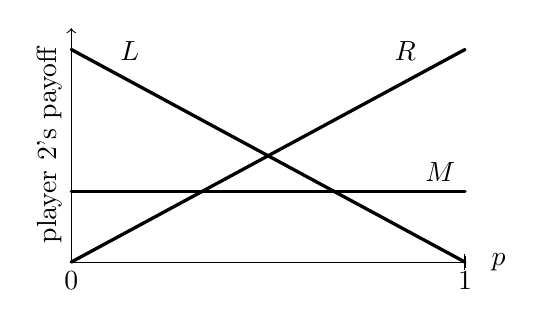
\begin{tikzpicture}[scale=1, line cap=round]

			% constants
			\pgfmathsetmacro{\xmax}{5};
			\pgfmathsetmacro{\ymax}{3};
			\pgfmathsetmacro{\ticklength}{1/14};
			\pgfmathsetmacro{\yscale}{0.9};
			\pgfmathsetmacro{\labelshift}{0.9};

			% x axis
			\draw[-|] (0,0) -- ( \xmax, 0.0 );
			\draw ( {\xmax+3*\ticklength}, 0.0 )
				node[anchor=west] {$p$};
			\draw[-] ( \xmax, - \ticklength )
				-- ( \xmax, \ticklength );
			\draw ( 0, 0.0 )
				node[anchor=north] {$0$};
			\draw ( \xmax, 0.0 )
				node[anchor=north] {$1$};

			% x axis
			\draw[->] (0,0) -- ( 0.0, {\yscale*1.1*\ymax} );
			\draw ( 0.0, {(\yscale*1.1*\ymax)/2} )
				node[anchor=east] {\rotatebox{90}{player~2's payoff}};

			% payoffs
			\draw[-,very thick] (0,0)
				-- ( \xmax, {\yscale*\ymax} );
			\draw[-,very thick] ( 0, { \yscale*\ymax} )
				-- ( \xmax, 0 );
			\draw[-,very thick] ( 0, {\yscale*\ymax/3} )
				-- ( \xmax, {\yscale*\ymax/3} );

			\draw ( {\labelshift*\xmax}, {\yscale*\labelshift*\ymax} )
				node[anchor=south east] {$R$};
			\draw ( {(1-\labelshift)*\xmax}, {\yscale*\labelshift*\ymax} )
				node[anchor=south west] {$L$};
			\draw ( \xmax, {\yscale*\ymax/3} )
				node[anchor=south east] {$M$};

		\end{tikzpicture}
		\caption{Player~2's action payoffs in \Cref{example:rbty_neverbest} as a function of the probability $p$ that player~1 plays $U$.}
		\label{fig:neverbest}
	\end{figure}
	%
	There is no $p \in [0,1]$ for which $M$ is weakly best, so $M$ is a never-best action.
	%
\end{example}

In the next section, we characterise rational play (i.e. sometimes-best actions) in terms of a seemingly different solution concept: strict dominance.



%%%%%%%%%%%%%%%%%%%%%%%%%%%%%%%%%%%
%%%%%%%%%%%%%%%%%%%%%%%%%%%%%%%%%%%
\section{Dominance}
\label{dom:dom}
%%%%%%%%%%%%%%%%%%%%%%%%%%%%%%%%%%%
%%%%%%%%%%%%%%%%%%%%%%%%%%%%%%%%%%%

\begin{definition}
	%
	\label{definition:dominates}
	%
	For mixed actions $\alpha_i,\beta_i \in \Delta(A_i)$ of a player $i \in I$, we say that $\alpha_i$ \emph{strictly dominates} $\beta_i$ iff $u_i(\alpha_i,a_{-i}) > u_i(\beta_i,a_{-i})$ for every (pure) profile $a_{-i} \in A_{-i}$ of other players' actions.
	%
\end{definition}

This definition covers strict dominance by/of pure actions, too, since pure actions $a_i,b_i \in A_i$ are a special case of mixed actions $\alpha_i,\beta_i \in \Delta(A_i)$ (namely, degenerate mixed actions).

\begin{example}
	%
	\label{example:prisoners}
	%
	Consider the prisoner's dilemma: players $I=\{1,2\}$, actions $A_1=A_2=\{C,D\}$ and payoffs
	%
	\begin{equation*}
		\begin{array}{c|ccc}
			  & C   & D   \\ \hline
			C & 2,2 & 0,3 \\
			D & 3,0 & 1,1
		\end{array}
	\end{equation*}
	%
	For both players, the action $C$ is strictly dominated by the (pure) action $D$.
	%
\end{example}

The fact that the definition quantifies only over pure profiles $a_{-i} \in A_{-i}$ does not matter: the alternative definition that quantifies over all mixed action profiles $\alpha_{-i} \in \Delta(A_{-i})$ is in fact equivalent.

\begin{exercise}[easy]
	%
	\label{exercise:dominates_others_mixed}
	%
	Prove it! That is, prove that for mixed actions $\alpha_i,\beta_i \in \Delta(A_i)$ of a player $i \in I$, $u_i(\alpha_i,a_{-i}) > u_i(\beta_i,a_{-i})$ for every pure profile $a_{-i} \in A_{-i}$ if and only if $u_i(\alpha_i,\alpha_{-i}) > u_i(\beta_i,\alpha_{-i})$ for every mixed profile $\alpha_{-i} \in \Delta(A_{-i})$.
	%
\end{exercise}

\begin{definition}
	%
	\label{definition:dominated}
	%
	A (pure) action $a_i \in A_i$ of player $i \in I$ is called \emph{strictly dominated} iff there is a mixed action $\beta_i \in \Delta(A_i)$ that strictly dominates $a_i$.%
		\footnote{One could extend the definition of `strictly dominated' to mixed actions $\alpha_i \in \Delta(A_i)$ in the obvious way, but that is typically not done.}
	%
\end{definition}

The fact that we contemplate strict domination by a \emph{mixed} action $\beta_i \in \Delta(A_i)$ matters: an action can easily be strictly dominated without being strictly dominated by a pure action.

\addtocounter{example}{-2}
\begin{example}[continued from \cpageref{example:rbty_neverbest}]
	%
	\label{example:rbty_neverbest_dom}
	%
	No pure action strictly dominates $M$:
	$M$ is better than $L$ against $U$, and better than $R$ against $D$. But $M$ is strictly dominated by a mixed action, namely the $50$--$50$ mix of $L$ and $R$: this mixed action yields an expected payoff of $1.5$ regardless of player~1's choice, strictly better than action $M$'s payoff of $1$.
	%
\end{example}
\addtocounter{example}{1}

% \begin{definition}
% 	%
% 	\label{definition:dominant}
% 	%
% 	A (pure) action $a_i \in A_i$ of player $i \in I$ is called \emph{strictly dominant} iff it strictly dominates every other (pure) action $b_i \in A_i \setminus \{a_i\}$.%
% 		\footnote{It makes no difference if we instead require $a_i$ to strictly dominate every other \emph{mixed} action $\beta_i \in \Delta(A_i) \setminus \{a_i\}$. Nor do we need to consider the possibility of a strictly dominant mixed action $\alpha_i \in A_i$, since an implication of such a definition would be that a strictly dominant action must be pure (why?).}
% 	%
% \end{definition}

Recall from the previous section that (Bayesian) rationality plus comprehension of the game entails nothing more or less than that no player plays a never-best action. The following shows that this is equivalent to eschewing strictly dominated actions.

\begin{namedthm}[Pearce's lemma.]
	%
	\label{lemma:pearce}
	%
	An action of a player is never-best if and only if it is strictly dominated.
	%
\end{namedthm}

\addtocounter{example}{-2}
\begin{example}[continued]
	%
	\label{example:rbty_neverbest_pearce}
	%
	We saw that player~2's action $M$ is never-best, and that it is strictly dominated. We also saw that player~2's other actions, $L$ and $R$, are sometimes-best (not never-best), and it may be verified that they are not strictly dominated. Similarly for both of player~1's actions, $U$ and $D$.
	%
\end{example}
\addtocounter{example}{1}

The proof relies on the separating hyperplane theorem.%
	\footnote{See e.g. Theorem~M.G.2 in \textcite[][p.~948]{MascolellWhinstonGreen1995}. For a fuller treatment, consider \textcite{Border2016}.}

\begin{proof}
	%
	For the `if' direction, suppose that $a_i$ is strictly dominated: there is a mixed action $\beta_i \in \Delta(A_i)$ such that $u_i(a_i,a_{-i}) < u_i(\beta_i,a_{-i})$ for all (pure) profiles $a_{-i} \in A_{-i}$. Then $u_i(a_i,\alpha_{-i}) < u_i(\beta_i,\alpha_{-i})$ for any conjecture $\alpha_{-i} \in \Delta(A_{-i})$, so $a_i$ is never-best.

	For the `only if' direction, we prove the contra-positive: we assume that $a_i$ is \emph{not} strictly dominated, and establish the existence of a conjecture $\alpha_{-i} \in \Delta(A_{-i})$ to which $a_i$ is a best reply (hence $a_i$ is not never-best). Enumerate the other players' action profiles $A_{-i}$ (a finite set) as $A_{-i} \equiv \{1,\dots,N\}$ where $N \coloneqq \abs*{A_{-i}}$. For each mixed action $\alpha_i \in \Delta(A_i)$, let $U^{\alpha_i} \in \R^N$ be the vector 
	%
	\begin{equation*}
		U^{\alpha_i} \coloneqq \bigl( u_i(\alpha_i,1), u_i(\alpha_i,2), \dots, u_i(\alpha_i,N) \bigr) ,
	\end{equation*}
	%
	and let
	%
	\begin{equation*}
		\mathcal{U} \coloneqq \left\{ v \in \R^N : \text{$v = U^{a_i} - U^{\alpha_i}$ for some $\alpha_i \in \Delta(A_i)$} \right\} .
	\end{equation*}
	%
	Observe that $\mathcal{U}$ is a convex subset of $\R^N$, and that $\boldsymbol{0} \coloneqq (0,0,\dots,0)$ is a member.%
		\footnote{For any $v,w \in \mathcal{U}$, we have $v = U^{a_i} - U^{\alpha_i}$ and $w = U^{a_i} - U^{\beta_i}$ for some $\alpha_i,\beta_i \in \Delta(A_i)$, which since $u_i(\cdot,n)$ is linear for each $n \in \{1,\dots,N\}$ implies that for any $\lambda \in (0,1)$, $\lambda v + (1-\lambda) w = U^{a_i} - U^{\lambda \alpha_i + (1-\lambda) \beta_i} \in \mathcal{U}$.}
	Since (by hypothesis) $a_i$ is not strictly dominated, it holds that for each $\alpha_i \in \Delta(A_i)$, there is an $n \in \{1,\dots,N\}$ such that $u_i(a_i,n) \geq u_i(\alpha_i,n)$; in other words, the $n$th entry of $U^{a_i}-U^{\alpha_i}$ is non-negative. Hence every element of $\mathcal{U}$ has at least one non-negative entry, which is to say that $\mathcal{U}$ is disjoint from the negative orthant
	%
	\begin{equation*}
		\R_{--}^N \coloneqq \{ v \in \R^N : \text{$v_n < 0$ for every $n \in \{1,\dots,N\}$} \} .
	\end{equation*}

	Since both $\mathcal{U}$ and $\R_{--}^N$ are convex, it follows by the separating hyperplane theorem that there exists a vector $v \in \R^N \setminus \{\boldsymbol{0}\}$ and a constant $c \in \R$ such that $u \cdot v \geq c$ for every $u \in \mathcal{U}$ and $u \cdot v \leq c$ for every $u \in \R_{--}^N$. It must be that $c=0$, since $\boldsymbol{0}$ belongs both to $\mathcal{U}$ and to the closure of $\R_{--}^N$.%
		\footnote{On the one hand, $c \leq \boldsymbol{0} \cdot v = 0$ since $u \in \mathcal{U}$. On the other hand, we have $c \geq (-\varepsilon,\dots,-\varepsilon) \cdot v$ for every $\varepsilon>0$ since $(-\varepsilon,\dots,-\varepsilon) \in \R_{--}^N$, so letting $\varepsilon \downarrow 0$ yields $c \geq \boldsymbol{0} \cdot v = 0$.}
	Furthermore, $v$ must have only non-negative entries, since otherwise we could find a $u \in \R_{--}^N$ such that $u \cdot v > 0$.%
		\footnote{If $v_n < 0$ for some $n \in \{1,\dots,N\}$, then $u \cdot v > 0$ for the vector $u \in \R_{--}^N$ defined by $u_n \coloneqq - 2 ( 1 + \sum_{m \neq n} \abs*{v_m} ) / (-v_n)$ and $u_m \coloneqq -1$ for each $m \in \{1,\dots,N\} \setminus \{n\}$.}
	Define
	%
	\begin{equation*}
		\alpha_{-i} \coloneqq \frac{v}{ \sum_{n=1}^N v_n } \in \Delta(A_{-i}) .
	\end{equation*}
	%
	The action $a_i$ is a best reply to the conjecture $\alpha_{-i}$, since for any other action $b_i \in A_i$, 
	%
	\begin{align*}
		u_i(a_i,\alpha_{-i})
		- u_i(b_i,\alpha_{-i})
		&= \sum_{n=1}^N
		\left[ u_i(a_i,n) - u_i(b_i,n) \right]
		\left[\alpha_{-i}\right]_n
		\\
		&= \left( U^{a_i} - U^{b_i} \right)
		\cdot \alpha_{-i}
		\geq 0 .
		\qedhere
	\end{align*}
	%
\end{proof}

\begin{remark}
	%
	\label{remark:pearce_finite}
	%
	The above proof relies on the assumption, maintained throughout this chapter, that the game under consideration is finite. 
	The `only if' part of \hyperref[lemma:pearce]{Pearce's lemma} is not generally true for non-finite games, as shown in \Cref{exercise:pearce_counterex} below. (The `if' part \emph{is} generally true.)
	It turns out, however, that the finiteness assumption in \hyperref[lemma:pearce]{Pearce's lemma} can be substituted with compactness of action sets and (upper semi-)continuity of payoffs.
	%
\end{remark}

\begin{exercise}
	%
	\label{exercise:pearce_counterex}
	%
	Consider the normal-form game $\left(I,(A_i,u_i)_{i \in I}\right)$ where $I = \{1,2\}$, $A_1 \coloneqq [0,1]$ and $A_2 = [0,1)$, and $u_1(a_1,a_2) \coloneqq - (a_1-a_2)^2$ for all $a_1 \in A_1$ and $a_2 \in A_2$.

	\begin{enumerate}[label=(\alph*)]
	
		\item Prove that player~1's action $a_1 = 1$ is never-best.

		\item Prove that player~1's action $a_1 = 1$ is \emph{not} strictly dominated. (Not even weakly dominated, in fact.)
	
	\end{enumerate}
	%
\end{exercise}



%%%%%%%%%%%%%%%%%%%%%%%%%%%%%%%%%%%
%%%%%%%%%%%%%%%%%%%%%%%%%%%%%%%%%%%
\section{Rationalisability}
\label{dom:rbty}
%%%%%%%%%%%%%%%%%%%%%%%%%%%%%%%%%%%
%%%%%%%%%%%%%%%%%%%%%%%%%%%%%%%%%%%

We have seen that the (only) implication of rationality and comprehension of the game is that players will not choose never-best (equivalently, strictly dominated) actions. But what if each player additionally knows that her opponents are rational?

\addtocounter{example}{-2}
\begin{example}[continued from \cpageref{example:rbty_neverbest,example:rbty_neverbest_dom,example:rbty_neverbest_pearce}]
	%
	\label{example:rbty_neverbest_rbty}
	%
	If player~2 is rational, then she will not play the never-best action $M$. Hence if player~1 knows that player~2 is rational, then she can rule out the possibility that player~2 will play $M$. Once the possibility of $M$ has been ruled out, rationality requires player~1 to choose action $D$, since it is strictly better than $U$ (payoff $1>0$) against player~2's remaining actions $\{L,R\}$. To summarise, rationality does \emph{not} require player~1 to chose $D$ (her other action $U$ is not never-best), but rationality plus knowledge of player~2's rationality does require player~1 to choose $D$.
	%
\end{example}
\addtocounter{example}{1}

Going further, it may be that each player $i \in I$ knows not only that players $j \in I \setminus \{i\}$ are rational, but also that players $j \in I \setminus \{i\}$ know that all players $k \in I \setminus \{j\}$ are rational.

\addtocounter{example}{-2}
\begin{example}[continued]
	%
	\label{example:rbty_neverbest_rbty1}
	%
	We saw that if player~1 is rational and knows that player~2 is rational, then she must play $D$. If in addition player~2 knows that player~1 knows than player~2 is rational, then player~2 understands that player~1 must play $D$. So if in addition player~2 is herself rational, she must play a best reply to $D$: in other words, she must play $L$. Thus rationality, knowledge of rationality and knowledge of knowledge of rationality together yield a unique prediction of play in this game.
	%
\end{example}
\addtocounter{example}{1}

Further still, it may be that for all players $i,j,k,\ell \in I$ such that $i \neq j \neq k \neq \ell$, player~$i$ knows not only that player~$j$ is rational and that player~$j$ knows that player~$k$ is rational, but also that player~$j$ knows that player~$k$ knows that player~$\ell$ is rational. And so on.

If all statements of the above form are true, we say that it is \emph{commonly known} that all players are rational; more concisely, there is `common knowledge of rationality'. The implications for play of rationality (of all players) and common knowledge (among all players) of rationality are precisely captured by \emph{rationalisability.}

\begin{definition}
	%
	\label{definition:rbty}
	%
	For each player $i \in I$ and each conjecture $\alpha_{-i} \in \Delta(A_{-i})$, write $\text{BR}_i(\alpha_{-i}) \subseteq A_i$ for the set of best replies to $\alpha_{-i}$.
	Define $X^0_i \coloneqq A_i$ and $X^0_{-i} \coloneqq A_{-i}$ for each $i \in I$.
	For each $t \in \N$, iteratively define
	%
	\begin{equation*}
		X^t_i \coloneqq \text{BR}_i\left( \Delta\left( X^{t-1}_{-i} \right) \right)
		\equiv \Union_{\alpha_{-i} \in \Delta\left( X^{t-1}_{-i} \right)} \text{BR}_i(\alpha_{-i})
		\quad \text{for each $i \in I$,}
	\end{equation*}
	%
	$X^t_{-j} \coloneqq \prod_{i \in I \setminus \{j\}} X^t_i$ for each $j \in I$, and $X^t \coloneqq \prod_{i \in I} X^t_i$.
	Finally, define $X^\infty_i \coloneqq \Intersect_{t \in \N} X^t_i$ for each $i \in I$, and $X^\infty \coloneqq \prod_{i \in I} X^\infty_i$. An action $a_i \in A_i$ of player $i \in I$ is called \emph{rationalisable} iff it belongs to $X^\infty_i$; similarly, an action profile $a = (a_i)_{i \in I} \in A$ is called rationalisable iff it belongs to $X^\infty$.
	%
\end{definition}

The procedure (or algorithm) described in \Cref{definition:rbty} is called \emph{iterated deletion of never-best actions.} By \hyperref[lemma:pearce]{Pearce's lemma}, it is equivalent to the more familiar procedure of \emph{iterated deletion of strictly dominated actions,} provided (crucially) that in each round, remaining actions that are strictly dominated by a remaining \emph{mixed} action are deleted.

\addtocounter{example}{-2}
\begin{example}[continued]
	%
	\label{example:rbty_neverbest_rbty2}
	%
	In the language of iterated deletion, our previous reasoning may be summarised as
	%
	\begin{align*}
		X^1 &= X^1_1 \times X^1_2 = \{U,D\} \times \{L,R\} ,
		\\
		X^2 &= X^2_1 \times X^2_2 = \{D\} \times \{L,R\} ,
		\\
		X^3 &= X^3_1 \times X^3_2 = \{D\} \times \{L\} ,
	\end{align*}
	%
	and $X^\infty = X^t = X^3$ for all $t \geq 4$. In particular, $D$ ($L$) is the unique rationalisable action of player~1 (player~2).
	%
\end{example}
\addtocounter{example}{1}

In the example, for each player $i \in I$, the sets $(X^t_i)_{t \in \N}$ are nested in the sense that $X^{t-1}_i \supseteq X^t_i$ for each $t \in \N$, and the set $X^\infty_i$ of rationalisable actions is non-empty. These features are general:

\begin{proposition}
	%
	\label{proposition:rbty_nonempty}
	%
	For each player $i \in I$, $X^{t-1}_i \supseteq X^t_i$ for each $t \in \N$, and the set $X^\infty_i$ of rationalisable actions is non-empty.
	%
\end{proposition}

This is a reassuring result, since if there were no rationalisable actions then we would be faced with the paradox that the game itself is somehow inconsistent with rationality and common knowledge of rationality!

\begin{proof}
	%
	We prove the first (nestedness) claim by induction on $t \in \N$.%
		\footnote{See \cref{math:pf} for a review of mathematical induction.}
	The base case $t=1$ is immediate: $X^0_i = A_i \supseteq X^1_i$ for every $i \in I$. For the induction step, fix any $t \in \N$, and suppose that $X^{t-1}_i \supseteq X^t_i$ for every player $i \in I$; we will show that $X^t_i \supseteq X^{t+1}_i$ for every player $i \in I$. So fix any player $i \in I$. Since $X^{t-1}_{-i} \supseteq X^t_{-i}$ (by the induction hypothesis), we have $\Delta(X^{t-1}_{-i}) \supseteq \Delta(X^t_{-i})$, and thus
	%
	\begin{equation*}
		X^t_i
		= \Union_{\alpha_{-i} \in \Delta(X^{t-1}_{-i})} \text{BR}_i(\alpha_{-i})
		\supseteq \Union_{\alpha_{-i} \in \Delta(X^t_{-i})} \text{BR}_i(\alpha_{-i})
		= X^{t+1}_i .
	\end{equation*}

	Toward proving the second (non-emptiness) claim, we first show that $X^t_i$ is non-empty for each $i \in I$ and $t \in \N$. We again employ induction on $t \in \{0,1,2,\dots\}$. For the base case $t=0$, obviously $X^0_i = A_i$ is non-empty for every $i \in I$. For the induction step, suppose for some $t \in \N$ that $X^{t-1}_i$ is non-empty for every $i \in I$; we will show that $X^t_i$ is also non-empty for every $i \in I$. To that end, fix any player $i \in I$ and an arbitrary element $\alpha_{-i}$ of the (by the induction hypothesis) non-empty set $\Delta(X^{t-1}_{-i})$. Since $A_i$ is (non-empty and) finite, there must be a best reply of player~$i$ to $\alpha_{-i}$. By definition, this best-reply action belongs to $X^t_i$; so $X^t_i$ is non-empty.

	We have shown that for each player $i \in I$, $A_i \supseteq X^{t-1}_i \supseteq X^t_i \neq \varnothing$ for every $t \in \N$. Since $A_i$ is finite for every player $i \in I$, it follows that the iteration must eventually terminate: $X^{T-1} = X^T \neq \varnothing$ for some $T \in \N$, so $X^t = X^{T-1}$ for all $t \geq T$. Then $X^\infty = X^{T-1} \neq \varnothing$.
	%
\end{proof}

\begin{remark}
	%
	\label{remark:rbty_nonempty_finite}
	%
	The above proof relies on the assumption, maintained throughout this chapter, that the game under consideration is finite.
	Like \hyperref[lemma:pearce]{Pearce's lemma}, \Cref{proposition:rbty_nonempty} remains true if action sets are allowed to be infinite, provided they are compact and payoffs are continuous. These hypotheses imply that $X^t_i$ is non-empty and closed for each $t \in \N$ and $i \in I$, and in fact also implies that $X^{t-1}_i \supseteq X^t_i$ for every $t \in \N$ and $i \in I$. The conclusion of \Cref{proposition:rbty_nonempty} then follows because the intersection of nested non-empty closed sets is necessarily non-empty (and closed).
	%
\end{remark}

In many (most?) games that arise in economics, rationalisability does not yield a unique prediction of play.

\begin{example}
	%
	\label{example:BoS}
	%
	Consider a $2 \times 2$ coordination game: players $I=\{1,2\}$, actions $A_1 = A_2 = \{B,S\}$, and payoffs
	%
	\begin{equation*}
		\begin{array}{c|cc}
			  & B        & S \\ \hline
			B & 1+\eps,1 & 0,\parbox{\widthof{$1+\eps$}}{\centering\vphantom{dp}$0$} \\
			S & \parbox{\widthof{$1+\eps$}}{\centering\vphantom{dp}$0$},0      & 1,1+\eps
		\end{array}
	\end{equation*}
	%
	where $\eps \geq 0$. Evidently neither player has a strictly dominated (=never-best) action, so every action of every player is rationalisable.
	%
\end{example}

However, there are economically important games in which rationalisability makes sharp predictions. In some cases, there is a \emph{unique} rationalisable action profile (such games are called \emph{dominance-solvable}). In such cases, stronger solution concepts such as Nash equilibrium (which make stronger assumptions about behaviour) are not required to obtain an unambiguous prediction of play.

\begin{exercise}
	%
	\label{exercise:nagel}
	%
	Each player $i \in \{1,\dots,\abs*{I}\}$ (where $\abs*{I} \geq 2$) chooses a number $a_i \in A_i \coloneqq \{1,2,3,\dots,99,100\}$. The `winners' are those whose choice is closest to $2/3$ of the average choice, i.e. those who chose
	%
	\begin{equation*}
		\text{best}((a_i)_{i \in I})
		\coloneqq \argmin_{n \in \left\{a_1,\dots,a_{\abs*{I}}\right\}}
		\abs*{ n - \frac{2}{3} \frac{1}{\abs*{I}} \sum_{j \in I} a_j } .
	\end{equation*}
	%
	The winners equally split a prize worth $1$, while the losers get nothing. Formally, each player~$i$'s payoff is
	%
	\begin{equation*}
		u_i(a_i,a_{-i})
		= \begin{cases}
			\left. 1 \middle/ \abs*{ \left\{ k \in I : a_k \in \text{best}\left((a_j)_{j \in I}\right) \right\} } \right.
			& \text{if $a_i \in \text{best}\left((a_j)_{j \in I}\right)$}
			\\
			0
			& \text{if $a_i \notin \text{best}\left((a_j)_{j \in I}\right)$.}
		\end{cases}
	\end{equation*}
	%
	This game is often interpreted as a formalisation of Keynes's (\citeyear{Keynes1936}, chapter~12) `beauty contest' model of financial speculation.
	Prove that every player has a unique rationalisable action (that is, there is an $n \in \{1,2,3,\dots,99,100\}$ such that $X^\infty_i = \{n\}$ for every player $i \in I$). (Take care!)
	%
\end{exercise}

\begin{example}
	%
	\label{example:cournot}
	%
	Consider the \textcite{Cournot1838} model of oligopolistic competition. Each of two firms $i \in I \coloneqq \{1,2\}$ chooses what quantity $a_i \in A_i \coloneqq \R_+$ to produce, earning profit 
	%
	\begin{equation*}
		u_i(a_i,a_{-i})
		\coloneqq a_i \times \left[ \kappa - \lambda(a_i+a_{-i}) - c \right] ,
	\end{equation*}
	%
	where $\kappa > c > 0 < \lambda$. The interpretation is that marginal cost is $c$ and that market inverse demand, i.e. price as a function of total quantity, is $q \mapsto \kappa - \lambda q$.
	Given quantities $(a_1,a_2) \in \R_+^2$, firm~$1$'s marginal gain from increasing its quantity is
	%
	\begin{equation*}
		f(a_1,a_2) \coloneqq
		\left. \frac{\dd}{\dd b_1}
		u_1(b_1,a_2)
		\right|_{b_1=a_1}
		= \kappa - c - 2 \lambda a_1 - \lambda a_2 .
	\end{equation*}
	%
	% Clearly for every $a_2 \in \R_+$, $f(\cdot,a_2)$ is strictly decreasing, so $u_2(\cdot,a_2)$ is strictly concave.

	Let $\overline{a}^1 \coloneqq (\kappa-c)/2\lambda$. Every action $a_1 > \overline{a}^1$ is strictly dominated by $\overline{a}^1$, since for every $a_2 \in \R_+$, $f(a_1,a_2) < 0$ for every $a_1 > \overline{a}^1$. By symmetry, every action $a_2 > \overline{a}^1$ is also strictly dominated. No other actions are strictly dominated, so $X^1_1 = X^1_2 = \left[ 0, \overline{a}^1 \right]$.

	Let $\underline{a}^2 \coloneqq \left( \kappa - c - \lambda \overline{a}_1 \right) / 2 \lambda$. For every remaining action $a_2 \in X^1_2$ of player~2, $f(a_1,a_2) > 0$ for every $a_1 < \underline{a}^2$, so $u_1\left( \underline{a}^2, a_2 \right) > u_1(a_1,a_2)$ for every $a_1 < \underline{a}^2$. No other actions of player~1 can be deleted, so $X^2_1 = \left[ \underline{a}^2, \overline{a}^1 \right]$. By symmetry, $X^2_2 = X^2_1 = \left[ \underline{a}^2, \overline{a}^1 \right]$.

	Continuing the argument,
	%
	\begin{equation*}
		X^3_1 = X^3_2
		= \left[ \underline{a}^2, \overline{a}^3 \right]
		\quad \text{where} \quad
		\overline{a}^3 \coloneqq \frac{ \kappa - c - \lambda \underline{a}^2 }{ 2 \lambda } ,
	\end{equation*}
	%
	whereupon
	%
	\begin{equation*}
		X^4_1 = X^4_2
		= \left[ \underline{a}^4, \overline{a}^3 \right]
		\quad \text{where} \quad
		\underline{a}^4 \coloneqq \frac{ \kappa - c - \lambda \overline{a}^3 }{ 2 \lambda } ,
	\end{equation*}
	%
	and so on. The general picture is that, letting $\underline{a}^0 \coloneqq 0$,
	%
	\begin{align*}
		X^n_1 = X^n_2
		&= \left[ \underline{a}^{n-1}, \overline{a}^n \right]
		\quad \text{where} \quad
		\overline{a}^n \coloneqq \frac{ \kappa - c - \lambda \underline{a}^{n-1} }{ 2 \lambda }
		\quad \text{for odd $n \in \N$,}
		\\
		X^n_1 = X^n_2
		&= \left[ \underline{a}^n, \overline{a}^{n-1} \right]
		\quad \text{where} \quad
		\underline{a}^n \coloneqq \frac{ \kappa - c - \lambda \overline{a}^{n-1} }{ 2 \lambda }
		\quad \text{for even $n \in \N$.}
	\end{align*}
	%
	It follows that the set of rationalisable actions is $X^\infty_1 = X^\infty_2 = \left[ \underline{a}^\infty, \overline{a}^\infty \right]$, where
	%
	\begin{equation*}
		\underline{a}^\infty
		\coloneqq \lim_{n \to \infty}
		\underline{a}^{2n}
		\quad \text{and} \quad
		\overline{a}^\infty
		\coloneqq \lim_{n \to \infty}
		\overline{a}^{2n-1} .
	\end{equation*}
	%
	(Both limits exist since the sequences are monotone: $(\underline{a}^{2n})_{n \in \N}$ is increasing, and $(\bar{a}^{2n-1})_{n \in \N}$ is decreasing.) It is easily verified that $\underline{a}^\infty = \bar{a}^\infty = a^\star \coloneqq (\kappa-c)/3\lambda$. So there is a unique rationalisable outcome: $X^\infty_1 = X^\infty_2 = \{a^\star\}$.
	%
\end{example}

\begin{exercise}
	%
	\label{exercise:hotelling}
	%
	Consider the \textcite{Hotelling1929} model of spatial competition, except discretised. Each of two firms $i \in I \coloneqq \{1,2\}$ chooses a location $a_i \in A_i \coloneqq \{0,1,2,3,\dots,99,100\}$. At each location $\in \{0,1,2,3,\dots,99,100\}$ there is a single consumer, who patronises whichever firm is located closer to her. If the firms are equidistant, then she randomises by tossing a fair coin. Firms earn a profit of £1 per customer who patronises them. (This implicitly assumes that the good is sold at an exogenous price that cannot be changed, and that marginal cost is constant.) Formally, the payoff of player $i \in I$ is
	%
	\begin{align*}
		u_i(a_i,a_{-i})
		\coloneqq{} &\abs*{ \left\{ \ell \in \{0,1,2,3,\dots,99,100\} : \abs*{ \ell - a_i } < \abs*{ \ell - a_{-i} } \right\} }
		\\
		+ \frac{1}{2} &\abs*{ \left\{ \ell \in \{0,1,2,3,\dots,99,100\} : \abs*{ \ell - a_i } = \abs*{ \ell - a_{-i} } \right\} } 
	\end{align*}
	%
	for all $(a_i,a_{-i}) \in A$. What are the rationalisable actions? (Bonus question: what if $A_1 = A_2 = [0,100]$?)
	%
\end{exercise}



%%%%%%%%%%%%%%%%%%%%%%%%%%%%%%%%%%%
%%%%%%%%%%%%%%%%%%%%%%%%%%%%%%%%%%%
\section{The best-reply property}
\label{dom:br_property}
%%%%%%%%%%%%%%%%%%%%%%%%%%%%%%%%%%%
%%%%%%%%%%%%%%%%%%%%%%%%%%%%%%%%%%%

In this section, we explore another formalisation (alternative to rationalisability) of the implications for play of rationality and common knowledge of rationality, based on the \emph{best-reply property.}

\begin{definition}
	%
	\label{definition:br_set}
	%
	A product set $Y = \prod_{i \in I} Y_i \subseteq A$ of action profiles has the \emph{best-reply property} iff for each player $i \in I$, every action $a_i \in Y_i$ is a best reply to some conjecture $\alpha_{-i} \in \Delta(Y_{-i})$ supported on $Y_{-i}$.
	%
\end{definition}

Sets with the best-reply property always exist, since $Y=\varnothing$ has the best-reply property.
A pure action profile $(a_i)_{i \in I} \in A$ is a Nash equilibrium if and only if the singleton $Y = \prod_{i \in I} \{a_i\} = \{(a_i)_{i \in I}\}$ has the best-reply property. More generally, if $(a^1_i)_{i \in I}, \dots, (a^N_i)_{i \in I} \in A$ are (pure-strategy) Nash equilibria, then $Y = \prod_{i \in I} \{a^1_i,\dots,a^N_i\}$ has the best-reply property.

\begin{observation}
	%
	\label{observation:br_property_max}
	%
	There is a largest set with the best-reply property. That is, there exists a set $Y^\star = \prod_{i \in I} Y^\star_i \subseteq A$ such that $Y^\star$ has the best-reply property and $Y^\star \supseteq Y$ for every set $Y = \prod_{i \in I} Y_i \subseteq A$ with the best-reply property.
	%
\end{observation}

\begin{proof}
	%
	By inspection, if $Y = \prod_{i \in I} Y_i \subseteq A$ and $Z = \prod_{i \in I} Z_i \subseteq A$ each have the best-reply property, then so does the player-wise union $\prod_{i \in I} ( Y_i \cup Z_i )$ of $Y$ and $Z$. Hence the player-wise union $Y^\star$ of \emph{all} sets with the best-reply property itself has the best-reply property, and by definition $Y^\star$ contains every set with the best-reply property.
	%
\end{proof}

The largest set with the best-reply property is the most permissive prediction of play which remains consistent with rationality and common knowledge thereof. It therefore intuitively captures the implications for play of rationality and common knowledge of rationality.

Rationalisability purported to formalise the same thing. We have thus ended up with two answers to the same question. The following result show that the two answers are, in fact, equivalent.

\begin{proposition}
	%
	\label{proposition:br_property}
	%
	The rationalisable set $X^\infty$ is the largest set with the best-reply property.
	%
\end{proposition}

\begin{proof}
	%
	Recall from \cpageref{definition:rbty} the definition, for each $t \in \N$ and each player $i \in I$, of the set $X^t_i \subseteq A_i$. Further recall that $X^\infty_i = \bigcap_{t \in \N} X^t_i$ for each player $i \in I$ and that $X^\infty = \prod_{i \in I} X^\infty_i$. By \Cref{proposition:rbty_nonempty} (since $A$ is finite), there is a $T \in \N$ such that $X^\infty = X^t = X^T$ for all $t \geq T$.
	
	To show that $X^\infty$ has the best-reply property, suppose toward a contradiction that for some player $i \in I$ and some rationalisable action $a_i \in X^\infty_i = X^T_i$ of hers, there is no conjecture $\alpha_{-i} \in \Delta(X^\infty_i) = \Delta(X^T_i)$ to which $a_i$ is a best reply. Then $a_i \notin X^{T+1}_i$ (by definition of $X^{T+1}_i$), which is contradicts the fact that $X^\infty = X^t = X^T$ for all $t \geq T$.

	It remains to show that $X^\infty$ is the largest set with the best-reply property. So fix any set $Y \subseteq \prod_{i \in I} Y_i \subseteq A$ with the best-reply property; we must show that $Y$ is contained in $X^t$ for every $t \in \{0,1,2,\dots\}$. We show this by induction on $t \in \{0,1,2,\dots\}$. The base case $t=0$ is immediate: $Y \subseteq A = X^0$. For the induction step, fix a $t \in \N$ and assume that $Y \subseteq X^{t-1}$; we must show that $Y \subseteq X^t$. By definition of $X^t = \prod_{i \in I} X^t_i$, it holds for every player $i \in I$ that $X^t_i$ contains \emph{every} best reply to any conjecture $\alpha_{-i} \in \Delta( X^{t-1}_{-i} ) \supseteq \Delta( Y_{-i} )$, where the inclusion holds by the induction hypothesis. And since $Y$ has the best-reply property, it must be (by definition) that every $a = (a_i)_{i \in I} \in Y$ is such that for each player $i \in I$, $a_i$ is a best reply to some conjecture $\alpha_{-i} \in \Delta( Y_{-i} )$. Thus $Y_i \subseteq X^t_i$ for every player $i \in I$, so $Y \subseteq X^t$.
	%
\end{proof}



%%%%%%%%%%%%%%%%%%%%%%%%%%%%%%%%%%%
%%%%%%%%%%%%%%%%%%%%%%%%%%%%%%%%%%%
\section{Independent conjectures}
\label{dom:indp}
%%%%%%%%%%%%%%%%%%%%%%%%%%%%%%%%%%%
%%%%%%%%%%%%%%%%%%%%%%%%%%%%%%%%%%%

Recall that we defined never-best actions and rationalisability allowing players to entertain conjectures about their opponents' play in which opponents' actions are correlated. In this section, we discuss how the analysis changes if we insist that players entertain only conjectures in which opponents' actions are statistically independent.

Note first of all that this makes no difference in two-player games, since then each player $i \in I$ has only one opponent. We focus for the rest of this section on games with three or more players.

Statistical independence of opponents' random actions formally means that each player $i \in I$ entertains only conjectures $\alpha_{-i} \in \Delta(A_{-i})$ that equal the product of their own marginals, i.e.
%
\begin{equation*}
	\alpha_{-i}(a_{-i})
	= \prod_{j \in I \setminus \{i\}} \alpha_j(a_j)
	\quad \text{for all $a_{-i} \equiv (a_j)_{j \in I \setminus \{i\}} \in A_{-i}$.}
\end{equation*}
%
We denote the set of such product-of-marginals conjectures of player $i \in I$ by $\Delta^\times(A_{-i}) \subseteq \Delta(A_{-i})$.

\begin{definition}
	%
	\label{definition:sbr_indep}
	%
	An action $a_i \in A_i$ of player $i \in I$ is \emph{$\times$-sometimes-best} iff there exists a conjecture $\alpha_{-i} \in \Delta^\times(A_{-i})$ such that $a_i$ is a best reply to $\alpha_{-i}$. An action that is not $\times$-sometimes-best is called \emph{$\times$-never-best.}
	%
\end{definition}

When there are three or more players, $\times$-never-best actions need not be never-best (hence by \hyperref[lemma:pearce]{Pearce's lemma}, they need not be strictly dominated):

\begin{example}[{\cite[p.~58]{OsborneRubinstein1994}}]
	%
	\label{example:rbty_indep}
	%
	Consider the following normal-form game with players $I = \{1,2,3\}$, in which player~1 chooses which row ($A_1 = \{U,D\}$), player~2 chooses which column ($A_2 = \{L,R\}$), and player~3 chooses which matrix ($A_3 = \{A,B,C,D\})$, and players' payoffs are equal:
	%
	\begin{equation*}
		\begin{aligned}
			&A:\\
			&\begin{array}{c|cc}
				  & L & R \\ \hline
				U & 8 & 0 \\
				D & 0 & 0
			\end{array}
		\end{aligned}
		\qquad
		\begin{aligned}
			&B:\\
			&\begin{array}{c|cc}
				  & L & R \\ \hline
				U & 4 & 0 \\
				D & 0 & 4
			\end{array}
		\end{aligned}
		\qquad
		\begin{aligned}
			&C:\\
			&\begin{array}{c|cc}
				  & L & R \\ \hline
				U & 0 & 0 \\
				D & 0 & 8
			\end{array}
		\end{aligned}
		\qquad
		\begin{aligned}
			&D:\\
			&\begin{array}{c|cc}
				  & L & R \\ \hline
				U & 3 & 3 \\
				D & 3 & 3
			\end{array}
		\end{aligned}
	\end{equation*}
	%
	Player~3's action $B$ is sometimes-best (i.e. not never-best): in particular, it is a best reply to the `correlated' conjecture according to which players $1$ and $2$ play either $(a_1,a_2) = (U,L)$ or $(a_1,a_2) = (D,R)$, each with equal probability.%
		\footnote{In symbols, $\alpha_{-3} \in \Delta(\{U,D\} \times \{L,R\})$ given by $\alpha_{-3}(U,L) = \alpha_{-3}(D,R) = 1/2$ and $\alpha_{-3}(D,L) = \alpha_{-3}(U,R) = 0$. Against this conjecture, action $B$ yields an expected payoff of $4$, the same as actions $A$ and $B$ and strictly better than the payoff $3$ of action $D$.}
	(It follows by \hyperref[lemma:pearce]{Pearce's lemma} that $B$ is not strictly dominated; this can also be checked directly.)
	However, $B$ is \emph{not} $\times$-sometimes-best: there is no `independent' conjecture $\alpha_{-3} \in \Delta^\times (\{U,D\} \times \{L,R\})$ to which $B$ is a best reply. That is because for any such `independent' conjecture, letting $p \in [0,1]$ denote the probability with which player~1 plays $U$ and $q \in [0,1]$ the probability with she plays $L$,
	the payoff of action $B$ is $4pq + 4(1-p)(1-q)$, which is
	strictly lower than the payoff $8pq$ of action $A$ if $p+q>1$,
	strictly lower than the payoff $8(1-p)(1-q)$ of action $C$ if $p+q<1$,
	and strictly lower than the payoff $3$ of action $D$ if $p+q=1$.
	%
\end{example}

The iterated deletion of $\times$-never-best actions, defined as in \Cref{definition:rbty} (\cpageref{definition:rbty}) except with only `independent' conjectures $\in \Delta^\times(A_{-i})$ considered at each step, leads to some set $X^{\infty,\times} = \prod_{i \in I} X^{\infty,\times}_i$ of action profiles. Call an action of player $i \in I$ \emph{$\times$-rationalisable} iff it belongs to $X^{\infty,\times}_i$. This concept is more restrictive than rationalisability.

\addtocounter{example}{-1}
\begin{example}[continued]
	%
	\label{example:rbty_indep_contd}
	%
	Evidently neither of player~1's actions is dominated, and (by symmetry) likewise for player~2. We saw that player~3's action $B$ is $\times$-never-best but not never-best. Hence $B$ is rationalisable, but not $\times$-rationalisable.
	%
\end{example}

A note on terminology: the term `rationalisability' is standardly used to refer both to what I have called `rationalisability' and to what I have called `$\times$-rationalisability'. One common way of distinguishing the two concepts is by calling them, respectively, `correlated rationalisability' and `independent rationalisability'. (My term `$\times$-rationalisability' is not standard.)



%%%%%%%%%%%%%%%%%%%%%%%%%%%%%%%%%%%
%%%%%%%%%%%%%%%%%%%%%%%%%%%%%%%%%%%
\section{Weak dominance}
\label{dom:weak_dom}
%%%%%%%%%%%%%%%%%%%%%%%%%%%%%%%%%%%
%%%%%%%%%%%%%%%%%%%%%%%%%%%%%%%%%%%

Strict dominance (equivalently, never-bestness) is demanding; perhaps too demanding.

\begin{example}
	%
	\label{example:idwds}
	%
	Consider the game with players $I = \{1,2\}$, actions $A_1 = \{U,D\}$ and $A_2 = \{L,R\}$, and payoffs
	%
	\begin{equation*}
		\begin{array}{c|cc}
			  & L   & R   \\ \hline
			U & 1,1 & 1,0 \\
			D & 1,1 & 0,0
		\end{array}
	\end{equation*}
	%
	Player~1's action $D$ is not strictly dominated (it is sometimes-best). But it would seem ill-advised for player~1 to play $D$: she loses nothing by playing $U$ instead, and in case player~2 plays $R$ then she gains strictly.
	%
\end{example}

The sense in which $D$ is worse than $U$ is called \emph{weak dominance.}

\begin{definition}
	%
	\label{definition:dominates_weak}
	%
	For mixed actions $\alpha_i,\beta_i \in \Delta(A_i)$ of a player $i \in I$, we say that $\alpha_i$ \emph{weakly dominates} $\beta_i$ iff $u_i(\alpha_i,a_{-i}) \geq u_i(\beta_i,a_{-i})$ for every (pure) profile $a_{-i} \in A_{-i}$ of other players' actions, with strict inequality for some profile.
	%
\end{definition}

\begin{definition}
	%
	\label{definition:dominated_weak}
	%
	A (pure) action $a_i \in A_i$ of player $i \in I$ is called \emph{weakly dominated} iff there is a mixed action $\beta_i \in \Delta(A_i)$ that weakly dominates $a_i$.
	%
\end{definition}

Weak dominance differs from strict dominance in that choosing a weakly dominated action \emph{need} not be strictly worse, though it \emph{may} be.

\addtocounter{example}{-1}
\begin{example}[continued]
	%
	\label{example:idwds_def}
	%
	Player~1's action $U$ weakly dominates $D$.
	%
\end{example}

Weak dominance is an attractive concept because choosing a weakly dominated action seems little better than choosing a strictly dominated one: at best, it would be incautious. This idea may be formalised as follows. Call a conjecture $\alpha_{-i} \in \Delta(A_{-i})$ of player $i \in I$ \emph{fully mixed} iff $\alpha_{-i}(a_{-i})>0$ for every profile $a_{-i} \in A_{-i}$ of other players' actions.

\begin{definition}
	%
	\label{definition:sbr_cautious}
	%
	An action $a_i \in A_i$ of player $i \in I$ is \emph{sometimes-cautiously-best} iff there exists a fully mixed conjecture $\alpha_{-i} \in \Delta(A_{-i})$ such that $a_i$ is a best reply to $\alpha_{-i}$. An action that is not sometimes-cautiously-best is called \emph{never-cautiously-best.}%
		\footnote{One could extend the definition of sometimes-best and never-best to mixed actions $\alpha_i \in \Delta(A_i)$ in the obvious way, but that is typically not done.}
	%
\end{definition}

\begin{namedthm}[Cautious Pearce's lemma.]
	%
	\label{lemma:pearce_cautious}
	%
	An action of a player is never-cautiously-best if and only if it is weakly dominated.
	%
\end{namedthm}

\begin{exercise}
	%
	\label{exercise:pearce_cautious_pf}
	%
	Prove it! (For a hint, see p.~64 of \textcite{OsborneRubinstein1994}.)
	%
\end{exercise}

\begin{example}
	%
	\label{example:voting}
	%
	Consider a complete-information voting game: each of finitely many voters votes for or against a proposal, the proposal passes iff a majority vote `for', and each voter $i$'s payoff is $v_i \in \R$ if the proposal passes and $0$ otherwise (the latter is a normalisation).
	Formally, the players are $I = \{1,2,\dots,2n+1\}$ for some $n \in \N$, actions are $A_i = \{ \text{for}, \text{against} \}$, and payoffs are
	%
	\begin{equation*}
		u_i((a_j)_{j \in I})
		=
		\begin{cases}
			v_i & \text{if $\abs*{\left\{ i \in I : a_i = \text{for} \right\}} \geq n+1$} \\
			0 & \text{if $\abs*{\left\{ i \in I : a_i = \text{for} \right\}} \leq n$}
		\end{cases}
		\quad \text{for each voter $i \in I$.}
	\end{equation*}
	%
	Every voter $i \in I$ who is not indifferent ($v_i \neq 0$) has a weakly dominant action: `for' if $v_i>0$, and `against' if $v_i<0$. No action of any player is strictly dominated, however.
	%
\end{example}

As with strict dominance, weak dominance can be applied iteratively. Iterated weak dominance is an alluring but dubious solution concept. A key drawback is that different predictions are obtained depending on the \emph{order} in which actions are deleted. (The same is not true of iterated strict dominance.)

\addtocounter{example}{-2}
\begin{example}[continued]
	%
	\label{example:idwds_iterated}
	%
	If we first delete player~1's weakly dominated action $D$, and then player~2's action $R$, we obtain the unique prediction $(U,L)$. If instead we first delete player~2's weakly (in fact strictly) dominated action $R$, then no further deletions based on weak dominance are possible, leaving us with \emph{two} predictions: $(U,L)$ and $(D,L)$.
	%
\end{example}
\addtocounter{example}{1}



%%%%%%%%%%%%%%%%%%%%%%%%%%%%%%%%%%%
%%%%%%%%%%%%%%%%%%%%%%%%%%%%%%%%%%%
\section{The literature}
\label{dom:lit}
%%%%%%%%%%%%%%%%%%%%%%%%%%%%%%%%%%%
%%%%%%%%%%%%%%%%%%%%%%%%%%%%%%%%%%%

The notions of dominance and best reply appeared early in the development of game theory: weak dominance was introduced by \textcite{Borel1921}, strict dominance figures in early work at the RAND Corporation (where the Prisoner's Dilemma was developed), and the notion of best reply is (I believe) due to \textcite{Nash1950,Nash1951}.

\hyperref[lemma:pearce]{Pearce's lemma} is from \textcite[][Lemma~3]{Pearce1984}. Similar results were known earlier; according to Bruno \textcite{Salcedo2020}, the earliest are those of \textcite{Wald1939,Stein1955}. \hyperref[lemma:pearce]{Pearce's lemma} is an instance of a more general (often useful) principle that `undominated' is equivalent to `optimal in some situation' \parencite[see e.g.][]{Fishburn1975,BorgersCheng2023}. The proof in the text (based on the separating-hyperplane theorem) is standard, but does not appear in \textcite{Pearce1984}; \textcite{Salcedo2020} attributes it to Abraham Wald.

Rationalisability was introduced by \textcite{Bernheim1984,Pearce1984}. Both authors considered both of the two definitions studied in this chapter, namely `the result of iterated deletion of never-best actions' and `largest set with the best-reply property', and proved non-emptiness and equivalence (\Cref{proposition:rbty_nonempty,proposition:br_property}). Bernheim also considered a third `epistemic' definition.

Both \textcite{Bernheim1984,Pearce1984} actually studied what I called `$\times$-rationalisability'; they called it simply `rationalisability', and it is nowadays often called `independent rationalisability'. What I called `rationalisability' was proposed by \textcite{BrandenburgerDekel1987} under the name `correlated rationalisability'.

We defined rationalisability only for normal-form games, but the idea extends to Bayesian games \parencite[see][]{DekelFudenbergMorris2007} and to extensive-form games \parencite[e.g.][]{Pearce1984,Battigalli1997,Battigalli2003,BattigalliSiniscalchi2003}.

For further/alternative reading, consider the textbook treatments in \textcite[chapter~4]{OsborneRubinstein1994}, \textcite[chapter~2]{FudenbergTirole1991} and \textcite[sections~1.8--1.9, 2.5 and 3.1]{Myerson1991}, and the lecture notes by \textcite{Salcedo2020}.



%%%%%%%%%%%%%%%%%%%%%%%%%%%%%%%%%%%
%%%%%%%%%%%%%%%%%%%%%%%%%%%%%%%%%%%
\section{More exercises}
\label{dom:exer}
%%%%%%%%%%%%%%%%%%%%%%%%%%%%%%%%%%%
%%%%%%%%%%%%%%%%%%%%%%%%%%%%%%%%%%%

\begin{exercise}
	%
	\label{exercise:bertrand_collusion}
	%
	Consider the \textcite{Bertrand1883} model of oligopolistic competition. Two firms $i \in I \coloneqq \{1,2\}$ produce the (exact) same good at marginal cost $c \geq 0$. The firms simultaneously choose prices $(a_1,a_2) \in A_1 \times A_2 = [0,\infty)^2$, whereupon a single consumer buys a single unit from whichever firm charges less. In case the firms' prices are equal, the consumer flips a fair coin. Formally, profits are
	%
	\begin{equation*}
		u_i(a_i,a_{-i})
		\coloneqq
		\begin{cases}
			a_i-c & \text{if $a_i < a_{-i}$} \\
			(a_i-c)/2 & \text{if $a_i = a_{-i}$} \\
			0 & \text{if $a_i > a_{-i}$.} 
		\end{cases}
	\end{equation*}

	\begin{enumerate}[label=(\alph*)]

		\item Show (or recall) that there is a symmetric pure-strategy Nash equilibrium in which both firms' profits are equal to $0$.

	\end{enumerate}

	For any $k \in (0,\infty)$ and $\ell \in [0,\infty)$, let $F_k^\ell : [0,\infty) \to [0,1]$ be defined by
	%
	\begin{equation*}
		F_k^\ell(x) \coloneqq
		\begin{cases}
			0 & \text{for $x \in [0,k+\ell)$} \\
			1 - k/(x-\ell) & \text{for $x \in [k+\ell,\infty)$.}
		\end{cases}
	\end{equation*}
	%
	Note that $F_k^\ell$ is a continuous CDF which is strictly increasing on $[k+\ell,\infty)$, i.e. $F_k^\ell(x) < F_k^\ell(x')$ whenever $k+\ell \leq x < x'$. In other words, it describes an atomless probability distribution with support $[k+\ell,\infty)$.

	\begin{enumerate}[label=(\alph*),resume]

		\item Show that for every $\pi \in (0,\infty)$, there is a symmetric mixed-strategy Nash equilibrium in which both firms' expected profits are equal to $\pi$.

		\item According to the internet,%
			\footnote{\url{https://library.fiveable.me/key-terms/principles-microeconomics/bertrand-model}}
		`The Bertrand model predicts that firms will price at marginal cost, resulting in a perfectly competitive outcome, even in an oligopolistic market.' Discuss.

		\item What are the rationalisable actions? (Be careful.)

		\item Show that if $c>0$, then there exist actions which are both rationalisable and weakly dominated.

	\end{enumerate}
	%
\end{exercise}

\begin{exercise}
	%
	\label{exercise:benporathdekel}
	%
	Consider the coordination game in Example~\ref*{example:BoS} (p.~\pageref*{example:BoS}) with $\varepsilon \coloneqq 4$, i.e. the payoff matrix is
	%
	\begin{equation*}
		\begin{array}{c|cc}
			  & B   & S \\ \hline
			B & 5,1 & 0,0 \\
			S & 0,0 & 1,5 
		\end{array}
	\end{equation*}
	%
	There are two pure-strategy Nash equilibria, $(B,B)$ and $(S,S)$; obviously player~1 strictly prefers the former.

	Suppose there is a prior stage at which player~1 can `burn (her own) money': specifically, she can choose `burn' and incur a payoff loss of $2$, or choose `don't (burn)' and incur no payoff loss. Player~1's choice is publicly observed before the coordination game is played.

	This is an extensive-form game, but we will study its `reduced normal form':%
		\footnote{For the general definition of the reduced normal form and an idea of why it matters, see e.g. \textcite[section~2.4]{Myerson1991}}
	the game in which player~1's actions are $A_1 \coloneqq \{\text{don't},\text{burn}\} \times \{B,S\}$ and player~2's are $A_2 \coloneqq \{B,S\}^2$, the interpretation being that player~1 chooses both whether to burn and whether to go $B$ or $S$ and that player~2 chooses both how to react to `don't' ($B$ or $S$) and how to react to `burn' ($B$ or $S$).

	\begin{enumerate}[label=(\alph*)]

		\item Complete the description of the normal-form game by writing down the ($4 \times 4$) payoff matrix.

		\item What are the pure-strategy Nash equilibria?

		\item Consider the following deletion procedure, called `maximal iterated deletion of weakly dominated actions.'

		\begin{enumerate}[label=(\roman*)]
		
			\item Delete all actions of either player which are weakly dominated. (There is just one, and it is actually \emph{strictly} dominated.)

			\item Delete all actions of either player which are (now) weakly dominated. (There are two.)

			\item Delete all actions of either player which are (now) weakly dominated. (There is just one, and it is actually \emph{strictly} dominated.)

			\item Delete all actions of either player which are (now) weakly dominated. (There is just one.)

			\item Delete all actions of either player which are (now) weakly dominated. (There is just one, and it is actually \emph{strictly} dominated.)
		
		\end{enumerate}
		%
		Which strategy profiles are left?

		\item Interpret. Will player~1 actually exercise her ability to burn money? Is the ability to burn money helpful, harmful or indifferent for player~1? Try to give an intuitive explanation.

	\end{enumerate}
	%
\end{exercise}

\begin{exercise}
	%
	\label{exercise:exam_ht25}
	%
	Consider the Bertrand model of oligopolistic competition, except with constraints on what prices can be charged. Two firms $i \in I \coloneqq \{1,2\}$ sell a homogeneous good, and choose what price $a_i \in A_i$ to charge, where $A_i$ is a non-empty subset of $[0,\infty)$. There is a single consumer, who buys from whichever firm charges less; if prices are equal, then the consumer randomises by tossing a fair coin. Firms' marginal costs are equal and constant, normalised to zero. Formally, the profit of each firm $i \in \{1,2\}$ is
	%
	\begin{equation*}
		u_i(a_i,a_{3-i})
		\coloneqq
		\begin{cases}
			a_i	& \text{if $a_i < a_{3-i}$}
			\\
			a_i/2	& \text{if $a_i = a_{3-i}$}
			\\
			0	& \text{if $a_i > a_{3-i}$.}
		\end{cases}
	\end{equation*}
	%
	Some reminders, in case you need them:
	
	\begin{itemize}

		\item `$\Delta(A_i)$' denotes the set of all probability distributions on $A_i$.

		\item An action $a_i \in A_i$ is a \emph{best reply} to a mixed action $\alpha_{3-i} \in \Delta(A_{3-i})$ if and only if $u_i(a_i,\alpha_{3-i}) \geq u_i(a_i',\alpha_{3-i})$ for every pure action $a_i' \in A_i$, where
		%
		\begin{equation*}
			u_i(a_i,\alpha_{3-i})
			\equiv \sum_{a_{3-i} \in A_{3-i}} u_i(a_i,a_{3-i}) \alpha_{3-i}(a_{3-i}) .
		\end{equation*}
	
		\item An action $a_i \in A_i$ of a player $i \in \{1,2\}$ is called \emph{never-best} if and only if there is no mixed action $\alpha_{3-i} \in \Delta(A_{3-i})$ to which $a_i$ is a best reply.

		\item An action $a_i \in A_i$ of a player $i \in \{1,2\}$ is \emph{strictly dominated} by a mixed action $\alpha_i \in \Delta(A_i)$ if and only if $u_i(a_i,a_{3-i}) < u_i(\alpha_i,a_{3-i})$ for every pure action $a_{3-i} \in A_{3-i}$, where
		%
		\begin{equation*}
			u_i(\alpha_i,a_{3-i})
			\equiv \sum_{a_i \in A_i} u_i(a_i,a_{3-i}) \alpha_i(a_i) .
		\end{equation*}

		\item Pearce's lemma says that if the action sets $A_1$ and $A_2$ are finite, then an action $a_i \in A_i$ of a player $i \in \{1,2\}$ is never-best if and only if it is strictly dominated by some mixed action $\alpha_i \in \Delta(A_i)$.

		\item The \emph{rationalisable} actions $X_1^\infty \subseteq A_1$ and $X_2^\infty \subseteq A_2$ are those actions that are left after all actions of either player that are never-best are deleted, and then all actions of either player that are (now) never-best are deleted, and so on forever.

	\end{itemize}
	%
	Answer the following.

	\begin{enumerate}[label=(\alph*)]

		\item Suppose that $0 \in A_1$ and $0 \in A_2$.

		\begin{enumerate}[label=(\roman*)]
		
			\item Show that no action is never-best. (That is, there is no player $i \in \{1,2\}$ and action $a_i \in A_i$ such that $a_i$ is never-best.)

			\item What are the rationalisable actions $X_1^\infty$ and $X_2^\infty$?
		
		\end{enumerate}

		\item Suppose that $A_1 = A_2 = \{1,2,3,4,\dots,K-1,K\}$, where $K$ is an integer that satisfies $K \geq 3$. (Note that $0 \notin A_1$ and $0 \notin A_2$.)

		\begin{enumerate}[label=(\roman*)]

			\item Show that $(a_1,a_2) = (2,2)$ is a Nash equilibrium.
		
			\item Show that $a_i = K$ is \emph{not} strictly dominated by the pure action $K-1$.

			\item Show that $a_i = K$ is never-best. (Take care.)

			\item What are the rationalisable actions $X_1^\infty$ and $X_2^\infty$? (Take care.)

		\end{enumerate}	

		\item Suppose that $A_1 = A_2 = [k,\infty)$ where $k>0$. Let $F_k$ denote the CDF $F_k : [0,\infty) \to [0,1]$ defined by
		%
		\begin{equation*}
			F_k(x) \coloneqq
			\begin{cases}
				0 & \text{for $x \in [0,k)$} \\
				1 - k/x & \text{for $x \in [k,\infty)$.}
			\end{cases}
		\end{equation*}
		%
		($F_k$ is called the `$\text{Pareto}(k,1)$ distribution'.)

		\begin{enumerate}[label=(\roman*)]
		
			\item Show that $(F_k,F_k)$ is a Nash equilibrium.

			\item What are the rationalisable actions $X_1^\infty$ and $X_2^\infty$?
		
		\end{enumerate}
	
	\end{enumerate}
	%
\end{exercise}





%%%%%%%%%%%%%%%%%%%%%%
%%%%%%%%%%%%%%%%%%%%%%
%%%%%%%%%%%%%%%%%%%%%%
\chapter{Tarski's fixed-point theorem}
\label{ch_tar}
%%%%%%%%%%%%%%%%%%%%%%
%%%%%%%%%%%%%%%%%%%%%%
%%%%%%%%%%%%%%%%%%%%%%

% Copyright (c) 2026 Carl Martin Ludvig Sinander.

% This program is free software: you can redistribute it and/or modify
% it under the terms of the GNU General Public License as published by
% the Free Software Foundation, either version 3 of the License, or
% (at your option) any later version.

% This program is distributed in the hope that it will be useful,
% but WITHOUT ANY WARRANTY; without even the implied warranty of
% MERCHANTABILITY or FITNESS FOR A PARTICULAR PURPOSE. See the
% GNU General Public License for more details.

% You should have received a copy of the GNU General Public License
% along with this program. If not, see <https://www.gnu.org/licenses/>.

%%%%%%%%%%%%%%%%%%%%%%%%%%%%%%%%%%%%%%%%%%%%%%%%%%%%%%%%%%%%%%%%%%%%%%%

Given a non-empty set $X$, a \emph{fixed point} of a map $f : X \to X$ is an $x \in X$ such that $f(x)=x$.
(For a correspondence $f : X \to 2^X$, a fixed point is any $x \in X$ such that $x \in f(x)$.)
Fixed points matter because nearly all equilibrium concepts in economics are precisely fixed points of some behavioural (often best-response-like) map $f : X \to X$; examples include Nash equilibrium, competitive equilibrium, and even rationalisability (see \cref{tar:app} below).

Fixed-point theorems are results which identify assumptions on $X$ and $f$ under which fixed points exist,%
	\footnote{This is non-trivial because many functions have no fixed point; the simplest example is the function $f : \{0,1\} \to \{0,1\}$ given by $f(0) \coloneqq 1$ and $f(1) \coloneqq 0$.}
and (sometimes) also describe the qualitative structure of the fixed-point set $\{ x \in X : f(x)=x \}$.
Three classic fixed-point theorems see extensive use in economics.

\begin{enumerate}

	\item \label{item:fpt_browuer} Brouwer's (\citeyear{Brouwer1912}) asserts that if $X$ is a non-empty, compact and convex subset of a Euclidean space and $f : X \to X$ is continuous, then $f$ has a fixed point. Famous applications include the proofs of the existence of Nash equilibrium \parencite{Nash1950,Nash1951} and of competitive equilibrium \parencite{Mckenzie1954,Mckenzie1959,ArrowDebreu1954}.

	\item \label{item:fpt_banach} Banach's (\citeyear{Banach1922}) asserts that if $(X,d)$ is a non-empty complete metric space and $f : X \to X$ is a contraction (there exists a $k \in [0,1)$ such that $d(f(x),f(y)) \leq k d(x,y)$ for all $x,y \in X$), then $f$ has exactly one fixed point, which may be found by iterating on $f$.%
		\footnote{`May be found by iterating on $f$' formally means that for any $x \in X$, $f^n(x)$ converges to the fixed point as $n \to \infty$, where $f^1 \coloneqq f$ and $f^{n+1} \coloneqq f \circ f^n$ for each $n \in \N$.}
	One famous application is the proof of the `principle of optimality' (the necessity and sufficiency of the Bellman equation) for infinite-horizon discounted dynamic programming \parencite{Blackwell1965}.

	\item \label{item:fpt_tarski} Tarski's (\citeyear{Tarski1955}) asserts that if $(X,\mathord{\lesssim})$ is a non-empty complete lattice and $f : X \to X$ is increasing, then the fixed-point set $\{ x \in X : f(x) = x \}$ is a non-empty complete lattice. This one is the subject of this chapter. It is perhaps less familiar than the other two, but it is just as useful; we shall see several applications in \cref{tar:app,ch_spm,ch_aps} below.

\end{enumerate}



%%%%%%%%%%%%%%%%%%%%%%%%%%%%%%%%%%%
%%%%%%%%%%%%%%%%%%%%%%%%%%%%%%%%%%%
\section{Partial orders}
\label{tar:poset}
%%%%%%%%%%%%%%%%%%%%%%%%%%%%%%%%%%%
%%%%%%%%%%%%%%%%%%%%%%%%%%%%%%%%%%%

Recall that given a set $X$, a \emph{binary relation} $\lesssim$ on $X$ is formally a subset of $X \times X$, though it is usual to write `$x \lesssim y$' in place of `$(x,y) \in \mathord{\lesssim}$'. The idea is that $x$ is in some general/abstract sense `weakly smaller' than $y$.

\begin{notation}
	%
	\label{notation:relations}
	%
	For a binary relation $\lesssim$ on a set $X$, we write
	%
	\begin{itemize}

		\item `$\gtrsim$' for the \emph{inverse} of $\lesssim$, meaning the binary relation on $X$ defined by, for all $x,y \in X$, $x \gtrsim y$ iff $y \lesssim x$,

		\item `$\not\lesssim$' for the \emph{complement} of $\lesssim$, meaning the binary relation on $X$ defined by, for all $x,y \in X$, $x \not\lesssim y$ iff it is not the case that $x \lesssim y$, and

		\item `$<$' for the \emph{strict part} of $\lesssim$, meaning the binary relation on $X$ defined by, for all $x,y \in X$, $x < y$ iff $x \lesssim y \not\lesssim x$.

	\end{itemize}
	%
\end{notation}

\begin{definition}
	%
	\label{definition:poset}
	%
	A binary relation on $X$ is called a \emph{partial order} iff it is transitive, reflexive and anti-symmetric.%
		\footnote{$\lesssim$ is \emph{transitive} iff for all $x,y,z \in X$, $x \lesssim y \lesssim z$ implies $x \lesssim z$, \emph{reflexive} iff $x \lesssim x$ for all $x \in X$, and \emph{anti-symmetric} iff for all $x,y \in X$, $x \lesssim y \lesssim x$ implies $x=y$.}
	A set $X$ equipped with a partial order $\lesssim$ is called a \emph{partially ordered set} (`poset' for short); we write `$(X,\mathord{\lesssim})$' when we are being fastidious, and simply `$X$' when we are not.
	%
\end{definition}

\begin{exercise}
	%
	\label{exercise:partial_orders}
	%
	Show the following:
	%
	\begin{enumerate}[label=(\alph*)]
	
		\item For $X \subseteq \R$, the ordinary inequality $\leq$ is a partial order on $X$.

		\item For $X \subseteq \R^n$ where $n \in \N$, the ordinary vector inequality $\leq$ is a partial order on $X$.

		\item When $X$ is a set of functions $\R \to \R$, pointwise inequality $\leq$ (i.e. $f \leq g$ iff $f(y) \leq g(y))$ for every $y \in \R$) is a partial order on $X$.

		\item For any non-empty set $S$, the containment relation $\subseteq$ is a partial order on the set $X \coloneqq 2^S$ of all subsets of $S$.

		\item \label{item:partial_orders:fosd} If $X$ is a set of CDFs on $\R$, then first-order stochastic dominance is a partial order on $X$. (Bonus question: same claim, but for second-order stochastic dominance.)

		\item \label{item:posets:pref} If $X$ is a non-empty set of alternatives and $\preceq$ is a preference relation on $X$ (a complete%
			\footnote{`Complete' means that for all $x,y \in X$, either $x \preceq y$ or $y \preceq x$.}
		and transitive binary relation), then $\preceq$ is a partial order if and only if it is never indifferent (there do not exist $x \neq y$ in $X$ such that $x \preceq y \preceq x$).

		\item Let $X$ be a non-empty set of alternatives, let $I$ be a non-empty set of agents, and let each agent $i \in I$ have a preference relation $\preceq_i$ over $X$. For $x,y \in X$, say that $x$ is \emph{weakly Pareto-dominated} by $y$ iff $x \preceq_i y$ for every $i \in I$. Show that `weakly Pareto-dominated by' is transitive and reflexive. What is the necessary and sufficient condition on the preference relations $(\mathord{\preceq}_i)_{i \in I}$ for `weakly Pareto-dominated by' to be a partial order?

		\item Fix a normal-form game $(I,(A_i,u_i)_{i \in I})$, and further fix a player $i \in I$. let $\lesssim_i$ be the binary relation on $A_i$ such that for any $a_i, b_i \in A_i$, it holds that $a_i \lesssim_i b_i$ iff either (1)~$a_i$ is weakly dominated by $b_i$ or (2)~$a_i$ and $b_i$ are payoff-equivalent, i.e. $u_i(a_i,a_{-i}) = u_i(b_i,a_{-i})$ for every $a_{-i} \in A_{-i}$. Show that $\lesssim_i$ is transitive and reflexive. What is the necessary and sufficient condition for $\lesssim_i$ to be a partial order?
	
	\end{enumerate}
	%
\end{exercise}

\begin{exercise}
	%
	\label{exercise:arrow-pratt}
	%
	Let $X$ be the set of all twice continuously differentiable functions $u : \R \to \R$ with strictly positive first derivative ($u'>0$). We interpret these as Bernoulli utility functions of expected-utility decision makers à la \textcite{VonneumannMorgenstern1947}. Recall that for $u,v \in X$, $u$ is called \emph{less risk-seeking than (or more risk-averse than) $v$} iff for any $x \in \R$ and any CDF $F$ on $\R$, $u(x) \leq \mathrel{(<)} \int u \dd F$ implies $v(x) \leq \mathrel{(<)} \int v \dd F$. (That is, whenever $u$ prefers a lottery $F$ to a sure thing $x$, so does $v$. This definition is due to \textcite{Yaari1969}.) Further recall that by the Arrow--Pratt theorem \parencite{Arrow1965,Pratt1964}, $u \in X$ is less risk-seeking than $v \in X$ iff $u'' / u' \leq v''/v'$.
	
	\begin{enumerate}[label=(\alph*)]
	
		\item Show that `less risk-seeking than' is transitive and reflexive, but not anti-symmetric, hence not a partial order on $X$.

	\end{enumerate}
	%
	Let $\mathcal{X}$ be the set of all equivalence classes of $X$ with respect to positive affine transformation; this just means that we identify (i.e. treat as identical) any two $u,v \in X$ such that $u = \alpha + \beta v$ for some $\alpha \in \R$ and $\beta \in \R_{++}$.

	\begin{enumerate}[label=(\alph*),resume]

		\item \label{item:arrow-pratt:b} Show that `less risk-seeking than' is a partial order on $\mathcal{X}$.
	
	\end{enumerate}
	%
\end{exercise}



%%%%%%%%%%%%%%%%%%%%%%%%%%%%%%%%%%%
%%%%%%%%%%%%%%%%%%%%%%%%%%%%%%%%%%%
\section{Lower and upper bounds, infima, suprema}
\label{tar:bounds}
%%%%%%%%%%%%%%%%%%%%%%%%%%%%%%%%%%%
%%%%%%%%%%%%%%%%%%%%%%%%%%%%%%%%%%%

\begin{definition}
	%
	\label{definition:lb}
	%
	Fix a poset $(X,\mathord{\lesssim})$ and a subset $S \subseteq X$. An element $x \in X$ is called a \emph{lower bound (in $(X,\mathord{\lesssim})$)} of $S$ iff $x \lesssim y$ for every $y \in S$.
	%
\end{definition}

\begin{exercise}
	%
	\label{exercise:lb-R}
	%
	Answer the following.
	
	\begin{enumerate}[label=(\alph*)]

		\item What are the lower bounds in $([0,1],\mathord{\leq})$ of $[1/2,1)$?

		\item What are the lower bounds in $([0,1],\mathord{\leq})$ of $(1/2,1)$?
	
		\item \label{item:lb_R_notsub} What are the lower bounds in $([0,1],\mathord{\leq})$ of $\{1/4\} \union (1/2,1)$?
	
	\end{enumerate}
	%
\end{exercise}

\begin{exercise}
	%
	\label{exercise:lb_disj}
	%
	Answer the following. (Think carefully about definitions.)
	
	\begin{enumerate}[label=(\alph*)]
	
		\item What are the lower bounds in $([0,1] \union [2,3],\mathord{\leq})$ of $(2,3]$?

		(Answer: $[0,1] \cup \{2\}$. Make sure that you understand why!)

		\item What are the lower bounds in $([0,1] \union (2,3],\mathord{\leq})$ of $(2,3]$?

		\item What are the lower bounds in $([0,1) \union (2,3],\mathord{\leq})$ of $(2,3]$?
	
	\end{enumerate}
	%
\end{exercise}

\begin{exercise}
	%
	\label{exercise:lb-R2}
	%
	Answer the following. (I suggest drawing pictures.)
	
	\begin{enumerate}[label=(\alph*)]
	
		\item \label{item:lb_R2:a} What are the lower bounds in $\left([0,1]^2,\mathord{\leq}\right)$ of $[1/2,1]^2$?

		\item \label{item:lb_R2:b} What are the lower bounds in $\left([0,1]^2,\mathord{\leq}\right)$ of $(1/2,1]^2$?

		\item \label{item:lb_R2:c} What are the lower bounds in $\left([0,1]^2,\mathord{\leq}\right)$ of $(1/4,1] \times [1/2,1]$?

		% \item What are the lower bounds in $\left([0,1]^2,\mathord{\leq}\right)$ of $\left\{ (x_1,x_2) \in [0,1]^2 : x_1 = x_2 \right\}$?

		\item \label{item:lb_R2:d} What are the lower bounds in $\left([0,1]^2,\mathord{\leq}\right)$ of
		%
		\begin{equation*}
			Y \coloneqq \left\{ (x_1,x_2) \in [0,1]^2 : x_1 + x_2 = 1 \right\} ?
		\end{equation*}

		\item \label{item:lb_R2:e} What are the lower bounds in $(Y,\mathord{\leq})$ of $\{(1/2,1/2)\}$?

		\item \label{item:lb_R2:f} What are the lower bounds in $(Y,\mathord{\leq})$ of $\{(1/3,2/3),(2/3,1/3)\}$?

		\item \label{item:lb_R2:g} What are the lower bounds in $(Y,\mathord{\leq})$ of $Y$?
	
	\end{enumerate}
	%
\end{exercise}

\begin{exercise}
	%
	\label{exercise:lb_exist}
	%
	Show that for any poset $(X,\mathord{\lesssim})$, the following are equivalent:

	\begin{itemize}
	
		\item Every set $S \subseteq X$ admits at least one lower bound in $(X,\mathord{\lesssim})$.

		\item $X$ has a $\lesssim$-least element (an $x \in X$ such that $x \lesssim y$ for every $y \in X$).
	
	\end{itemize}
	%
\end{exercise}

\begin{exercise}
	%
	\label{exercise:lb_empty}
	%
	Fix an arbitrary poset $(X,\mathord{\lesssim})$, and let $S \coloneqq \varnothing$ (the empty set). What are the lower bounds in $(X,\mathord{\lesssim})$ of $S$?
	%
\end{exercise}

\begin{definition}
	%
	\label{definition:glb}
	%
	Fix a poset $(X,\mathord{\lesssim})$ and a subset $S \subseteq X$.
	An element $x \in X$ is called the \emph{infimum (in $(X,\mathord{\lesssim})$)} of $S$ iff $x$ is a lower bound (in $(X,\mathord{\lesssim})$) of $S$ and $y \lesssim x$ for every lower bound $y \in X$ (in $(X,\mathord{\lesssim})$) of $S$.
	The infimum (in $(X,\mathord{\lesssim})$) of $S$, if it exists, is denoted `$\inf_{(X,\mathord{\lesssim})} S$' when we are being fastidious, and simply `$\inf S$' when we are not.%
		\footnote{Other names for infima are `greatest lower bound', `meet', `$\bigwedge_{(X,\mathord{\lesssim})} S$' and `$\bigwedge S$'.}
	%
\end{definition}

We say `the' infimum for a reason:

\begin{exercise}
	%
	\label{exercise:glb_unique}
	%
	Fix a poset $(X,\mathord{\lesssim})$ and a subset $S \subseteq X$. Prove that the infimum of $S$ is unique if it exists. (In other words: $S$ has at most one infimum.) (Hint: recall the definition of a partial order.)
	%
\end{exercise}

\begin{namedthm}[\Cref*{exercise:lb-R} {\normalfont (continued)}.]
	%
	\label{exercise:lb-R-latt}
	%
	Revisit each part and identify the infimum.
	%
\end{namedthm}

\begin{namedthm}[\Cref*{exercise:lb_disj} {\normalfont (continued)}.]
	%
	\label{exercise:lb_disj_latt}
	%
	Revisit each part and determine whether there is an infimum, and if yes, what it is. (Hint: in at least one part, no infimum exists.)
	%
\end{namedthm}

\begin{exercise}
	%
	\label{exercise:lb-R_sublatt}
	%
	Prove the following.

	\begin{enumerate}[label=(\alph*)]

		\item `Infimum in $(\R,\mathord{\leq})$' as defined by \Cref{definition:glb} above is equivalent to the familiar notion of `infimum' from real analysis: that is, $\inf_{(\R,\mathord{\leq})} S = \inf S$ for every non-empty $S \subseteq \R$ that is bounded below.%
			\footnote{`Bounded below' means that there is an $x \in \R$ such that $x \leq y$ for every $y \in S$.}

		\item \label{item:lb_R_sublatt:ineq} For any $X \subseteq \R$,
		$\inf_{(X,\mathord{\leq})} S 
		\leq \inf_{(\R,\mathord{\leq})} S
		= \inf S$ for every non-empty $S \subseteq X$ that is bounded below.

		\item \label{item:lb_R_sublatt:subcompl} For any compact $X \subseteq \R$,
		$\inf_{(X,\mathord{\leq})} S 
		= \inf_{(\R,\mathord{\leq})} S
		= \inf S$ for every non-empty $S \subseteq X$.

		\item There exist $S \subseteq X \subseteq \R$ such that $S$ is bounded below and
		$\inf_{(X,\mathord{\leq})} S 
		< \inf_{(\R,\mathord{\leq})} S
		= \inf S$.
		(Hint: take inspiration from \Cref{exercise:lb-R}\ref{item:lb_R_notsub} on \cpageref{item:lb_R_notsub}.)
	
	\end{enumerate}
	%
\end{exercise}

\begin{exercise}
	%
	\label{exercise:lb_sublat}
	%
	Prove the following generalisation of \Cref{exercise:lb-R_sublatt}\ref{item:lb_R_sublatt:ineq}--\ref{item:lb_R_sublatt:subcompl}: for any poset $(X,\mathord{\lesssim})$ and any $S \subseteq Y \subseteq X$, if $\inf_{(Y,\mathord{\lesssim})} S$ and $\inf_{(X,\mathord{\lesssim})} S$ exist, then $\inf_{(Y,\mathord{\lesssim})} S \lesssim \inf_{(X,\mathord{\lesssim})} S$, and if in addition $\inf_{(X,\mathord{\lesssim})} S$ belongs to $Y$, then $\inf_{(Y,\mathord{\lesssim})} S = \inf_{(X,\mathord{\lesssim})} S$.
	%
\end{exercise}

\begin{namedthm}[\Cref*{exercise:lb-R2} {\normalfont (continued)}.]
	%
	\label{exercise:lb-R2_latt}
	%
	Revisit each part and determine whether there is an infimum, and if yes, what it is.
	%
\end{namedthm}

\begin{namedthm}[\Cref*{exercise:lb_exist} {\normalfont (continued)}.]
	%
	\label{exercise:lb_exist_latt}
	%
	Show that for any poset $(X,\mathord{\lesssim})$, the set $X$ has a $\lesssim$-least element iff $X$ has an infimum in $(X,\mathord{\lesssim})$.
	%
\end{namedthm}

\begin{definition}
	%
	\label{definition:ub_lub}
	%
	Fix a poset $(X,\mathord{\lesssim})$ and a subset $S \subseteq X$. An element $x \in X$ is called an \emph{upper bound (in $(X,\mathord{\lesssim})$)} of $S$ iff $y \lesssim x$ for every $y \in S$.%
		\footnote{Equivalently, $x \in X$ is an upper bound in $(X,\mathord{\lesssim})$ of $S$ iff it is a lower bound in $(X,\mathord{\gtrsim})$ of $S$.}
	An element $x \in X$ is called the \emph{supremum (in $(X,\mathord{\lesssim})$)} of $S$ iff $x$ is an upper bound (in $(X,\mathord{\lesssim})$) of $S$ and $x \lesssim y$ for every upper bound $y \in X$ (in $(X,\mathord{\lesssim})$) of $S$.%
		\footnote{Equivalently, $x \in X$ is the supremum in $(X,\mathord{\lesssim})$ of $S$ iff it is the infimum in $(X,\mathord{\gtrsim})$ of $S$.}
	The supremum (in $(X,\mathord{\lesssim})$) of $S$, if it exists, is denoted `$\sup_{(X,\mathord{\lesssim})} S$'.%
		\footnote{Other names for suprema are `least upper bound', `join', $\bigvee_{(X,\mathord{\lesssim})} S$ and `$\bigvee S$'.}
	%
\end{definition}

\begin{namedthm}[\Cref*{exercise:lb_exist} {\normalfont (continued)}.]
	%
	\label{exercise:ub_exist_latt}
	%
	Fix an arbitrary poset $(X,\mathord{\lesssim})$. Show that $X$ has a supremum in $(X,\mathord{\lesssim})$ iff $X$ has a $\lesssim$-greatest element (an $x \in X$ such that $y \lesssim x$ for every $y \in X$).
	%
\end{namedthm}

\begin{namedthm}[\Cref*{exercise:lb-R} {\normalfont (continued)}.]
	%
	\label{exercise:lb-R-upp}
	%
	In each case, what are the \emph{upper} bounds?
	%
\end{namedthm}



%%%%%%%%%%%%%%%%%%%%%%%%%%%%%%%%%%%
%%%%%%%%%%%%%%%%%%%%%%%%%%%%%%%%%%%
\section{Lattices}
\label{tar:latt}
%%%%%%%%%%%%%%%%%%%%%%%%%%%%%%%%%%%
%%%%%%%%%%%%%%%%%%%%%%%%%%%%%%%%%%%

\begin{definition}
	%
	\label{definition:lattice}
	%
	A poset $(X,\mathord{\lesssim})$ is called a \emph{lattice} iff every two-element set $S = \{x,y\} \subseteq X$ has an infimum and a supremum, and is called a \emph{complete lattice} iff every set $S \subseteq X$ has an infimum and a supremum.
	%
\end{definition}

It is common to abbreviate `$(X,\mathord{\lesssim})$ is a (complete) lattice' to `$X$ is a (complete) lattice', leaving the partial order $\lesssim$ implicit. I will avoid this, as it can be confusing.

\begin{example}
	%
	\label{example:meet_boolean}
	%
	For any non-empty set $S$, the \emph{Boolean lattice} $\bigl( 2^S, \mathord{\subseteq} \bigr)$ is, as its name suggests, a lattice. In particular, for any subsets $R,T \subseteq S$,
	%
	\begin{equation*}
		\inf_{\left( 2^S, \mathord{\subseteq} \right)}\{ R, T \}
		= R \cap T
		\quad \text{and} \quad
		\sup_{\left( 2^S, \mathord{\subseteq} \right)}\{ R, T \}
		= R \cup T .
	\end{equation*}
	%
	Actually, it is a \emph{complete} lattice, with
	%
	\begin{equation*}
		\inf_{\left( 2^S, \mathord{\subseteq} \right)}\mathcal{R}
		= \bigcap_{R \in \mathcal{R}} R
		\quad \text{and} \quad
		\sup_{\left( 2^S, \mathord{\subseteq} \right)}\mathcal{R}
		= \bigcup_{R \in \mathcal{R}} R 
	\end{equation*}
	%
	for each collection $\mathcal{R} \subseteq 2^S$ of subsets of $S$.
	%
\end{example}

\begin{namedthm}[\Cref*{exercise:lb-R} {\normalfont (continued)}.]
	%
	\label{exercise:lb-R-lat}
	%
	Is $([0,1],\mathord{\leq})$ a lattice? Is it a complete lattice?
	%
\end{namedthm}

\begin{namedthm}[\Cref*{exercise:lb_disj} {\normalfont (continued)}.]
	%
	\label{exercise:lb_disj_lat}
	%
	Answer the following.
	
	\begin{enumerate}[label=(\alph*)]
	
		\item Is $([0,1] \union [2,3],\mathord{\leq})$ a lattice? Is it a complete lattice?

		\item Is $([0,1] \union (2,3],\mathord{\leq})$ a lattice? Is it a complete lattice?

		\item Is $([0,1) \union (2,3],\mathord{\leq})$ a lattice? Is it a complete lattice?
	
	\end{enumerate}
	%
\end{namedthm}

\begin{namedthm}[\Cref*{exercise:lb-R2}\ref*{item:lb_R2:a}--\ref*{item:lb_R2:d} {\normalfont (continued)}.]
	%
	\label{exercise:lb-R2_lat_a-d}
	%
	Show that the infimum in $\left( [0,1]^2, \mathord{\leq} \right)$ of any set $S \subseteq [0,1]^2$ exists and is equal to the `coordinate-by-coordinate' infimum, i.e. the vector $\bigl( \inf_{([0,1],\mathord{\leq})} S_1, \inf_{([0,1],\mathord{\leq})} S_2 \bigr)$ where
	%
	\begin{align*}
		S_1 &\coloneqq \left\{ x_1 \in [0,1] : \text{$(x_1,x_2) \in S$ for some $x_2 \in [0,1]$} \right\}
		\quad \text{and}
		\\
		S_2 &\coloneqq \left\{ x_2 \in [0,1] : \text{$(x_1,x_2) \in S$ for some $x_1 \in [0,1]$} \right\} .
	\end{align*}
	%
	Further show that $\left( [0,1]^2, \mathord{\leq} \right)$ is a complete lattice.
	%
\end{namedthm}

$\left( \R^2, \mathord{\leq} \right)$ is an example of a \emph{product lattice:} a poset $(X,\mathord{\lesssim})$ such that $X = \prod_{i \in \mathcal{I}} X_i$, where $X_i \subseteq \R$ for each $i \in \mathcal{I}$ (and where $\mathcal{I}$ is a non-empty [`index'] set), and for any $x = (x_i)_{i \in \mathcal{I}} \in X$ and $y = (y_i)_{i \in \mathcal{I}} \in X$, it holds that $x \lesssim y$ iff $x_i \leq y_i$ for every $i \in \mathcal{I}$. As the name suggests, every product lattice is a lattice. Another example of a product lattice is the set of all functions $\R \to \R$ ordered by `pointwise inequality' $\leq$, i.e. $f \leq g$ iff $f(y) \leq g(y)$ for every $y \in \R$. (In this case, the `index' set is $\mathcal{I} \coloneqq \R$, and $x_i \equiv f(i)$ for each $i \in \mathcal{I}$.)

It is a general fact that for a product lattice $(X,\mathord{\lesssim}) = \left( \prod_{i \in \mathcal{I}} X_i, \mathord{\lesssim} \right)$, the infimum and supremum in $(X,\mathord{\lesssim})$ of any set $S \subseteq X$, if these exist, are equal to $\bigl( \inf_{(X_i,\mathord{\leq})} S_i \bigr)_{i \in \mathcal{I}}$ and $\bigl( \sup_{(X_i,\mathord{\leq})} S_i \bigr)_{i \in \mathcal{I}}$, where
%
\begin{equation*}
	S_i \coloneqq \left\{ x_i \in X_i : \text{$(x_i,x_{-i}) \in S$ for some $x_{-i} \in \prod_{j \in \mathcal{I} \setminus \{i\}} X_j$} \right\} .
\end{equation*}
%
If $X_i$ is compact for each $i \in \mathcal{I}$, then by \Cref{exercise:lb-R_sublatt}\ref{item:lb_R_sublatt:subcompl}, we may replace the `$\inf_{(X_i,\mathord{\leq})}$' and `$\sup_{(X_i,\mathord{\leq})}$' with the ordinary `$\inf$' and `$\sup$' from real analysis.

\begin{exercise}
	%
	\label{exercise:product_compl_lattice}
	%
	Consider the product lattice $(X,\mathord{\leq})$, where $X \coloneqq \prod_{i \in \mathcal{I}} X_i$, the set $\mathcal{I}$ is non-empty, and $X_i \subseteq \R$ for each $i \in \mathcal{I}$. Prove that if $X_i$ is compact for each $i \in \mathcal{I}$, then $(X,\mathord{\leq})$ is a complete lattice.
	%
\end{exercise}

\begin{namedthm}[\Cref*{exercise:lb-R2}\ref*{item:lb_R2:e}--\ref*{item:lb_R2:g} {\normalfont (continued)}.]
	%
	\label{exercise:lb-R2_lat_e-g}
	%
	Recall that
	%
	\begin{equation*}
		Y \coloneqq \left\{ (x_1,x_2) \in [0,1]^2 : x_1 + x_2 = 1 \right\} .
	\end{equation*}
	%
	Is $( Y, \mathord{\leq} )$ a lattice? Is it a complete lattice?
	%
\end{namedthm}

\begin{exercise}
	%
	\label{exercise:budget_set_latt}
	%
	Consider the standard consumer-choice problem. There are $L \geq 2$ goods, whose prices are $p \in \R_{++}^L$. The consumer has income/wealth $w \in \R_{++}$, and chooses her consumption $x \in \R_+^L$ of each good. Hence her budget set is $B \coloneqq \left\{ x \in \R_+^L : p \cdot x \leq w \right\}$.

	\begin{enumerate}[label=(\alph*)]
	
		\item Let `$\leq$' denote the standard `coordinate-wise' order on $B$ (that is, $x \leq y$ iff $x_\ell \leq y_\ell$ for each good $\ell \in \{1,\dots,L\}$). Is $(B,\mathord{\leq})$ a lattice?

		\item Assume that $L \coloneq 2$, and let $\lesssim$ be the partial order defined by $(x_1,x_2) \lesssim (y_1,y_2)$ iff $x_1 \leq y_1$ and $x_2 \geq y_2$. Show that $(B,\mathord{\lesssim})$ is a complete lattice.
	
	\end{enumerate}
	
	%
\end{exercise}

\begin{namedthm}[\Cref*{exercise:lb_empty} {\normalfont (continued)}.]
	%
	\label{exercise:lb_empty_lat}
	%
	Let $X \coloneqq \varnothing$. There is exactly one partial order on $X$; why? Call this partial order $\lesssim$. $(X,\mathord{\lesssim})$ is a lattice; why?
	%
\end{namedthm}

\begin{exercise}
	%
	\label{exercise:diamond}
	%
	Let $X = \left\{ (0,0), (1,2), (2,1), (3,3) \right\} \subseteq \R^2$, and let $\leq$ be the usual coordinate-wise order, i.e. $(x_1,x_2) \leq (y_1,y_2)$ if and only if $x_1 \leq y_1$ and $x_2 \leq y_2$. (Draw a picture, probably.)
	
	\begin{enumerate}[label=(\alph*)]
	
		\item What is the infimum in $(X,\mathord{\leq})$ of $S = \{ (1,2), (2,1) \}$? (Answer: $(0,0)$. Not $(1,1)$! Make sure that you understand why.)

		\item Is $(X,\mathord{\leq})$ a lattice?
	
	\end{enumerate}
	%
\end{exercise}

\begin{exercise}
	%
	\label{exercise:latt_compl_finite}
	%
	Let $(X,\mathord{\lesssim})$ be a poset, and assume that $X$ is finite. Prove that $(X,\mathord{\lesssim})$ is a complete lattice iff it is a lattice. (Bonus question: show by example that this equivalence can fail if $X$ is not assumed finite.)
	%
\end{exercise}

\begin{namedthm}[\Cref*{exercise:arrow-pratt}\ref*{item:arrow-pratt:b} {\normalfont (continued from \cpageref{exercise:arrow-pratt,item:arrow-pratt:b})}.]
	%
	\label{exercise:arrow-pratt_lattice}
	%
	Show that the poset $\left(\mathcal{X},\text{`less risk-seeking than'}\right)$ is a lattice.
	%
\end{namedthm}

\begin{exercise}[brace yourself]
	%
	\label{exercise:CDFs_lattice}
	%
	Let $X$ be the set of all CDFs on $\R$. In other words, $X$ is the set of all increasing and right-continuous functions $F : \R \to [0,1]$ that satisfy $\lim_{y \downarrow -\infty} F(y) = 0$ and $\lim_{y \uparrow +\infty} F(y) = 1$.
	For any $F,G \in X$, write $F \lesssim G$ iff $F$ is first-order stochastically dominated by $G$ (that is, $F(y) \geq G(y)$ for every $y \in \R$). We know from \Cref{exercise:partial_orders}\ref{item:partial_orders:fosd} (\cpageref{item:partial_orders:fosd}) that $(X,\mathord{\lesssim})$ is a poset.

	\begin{enumerate}[label=(\alph*)]
	
		\item Show that $(X,\mathord{\lesssim})$ is a lattice, and give explicit expressions for the infimum and supremum of an arbitrary two-element set $\{F,G\} \subseteq X$.
	
	\end{enumerate}
	%
	In the rest of this exercise, we prove that the lattice $(X,\mathord{\lesssim})$ is not complete, and ask which sets $S \subseteq X$ \emph{do} admit an infimum and supremum. This requires some more mathematical concepts.

	Recall that a function $\phi : \R \to [0,1]$ is called \emph{upper semi-continuous (USC)} iff $\limsup_{z \to y} \phi(z) \leq \phi(y)$ for each $y \in \R$. Equivalently, $\phi : \R \to [0,1]$ is USC iff for any $k \in [0,1]$, the set $\left\{ y \in \R : \phi(y) \geq k \right\}$ is closed.
	A key fact about USC functions is that for any collection $\Phi$ of USC functions $\R \to [0,1]$, the `pointwise infimum', i.e. the function $\psi : \R \to [0,1]$ defined by $\psi(y) \coloneqq \inf_{\phi \in \Phi} \phi(y)$ for each $y \in \R$, is USC.%
		\footnote{\emph{Proof.}\, For any $k \in \R$, $\left\{ y \in \R : \psi(y) \geq k \right\} = \Intersect_{\phi \in \Phi} \left\{ y \in \R : \phi(y) \geq k \right\}$, which is closed since each $\phi \in \Phi$ is USC and since the intersection of closed sets is closed. \qed}
	The same is \emph{not} true of the `pointwise supremum'.%
		\footnote{Consider $\Phi = \{ \1_{[z,\infty)} : z \in \R_{++} \}$ where, recall, `$\R_{++}$' are the strictly positive real numbers and `$\1_S$' for $S \subseteq \R$ is the function $\R \to [0,1]$ defined by $\1_S(y) \coloneqq 1$ for $y \in S$ and $\1_S(y) \coloneqq 0$ for $y \in \R \setminus S$.}

	For any function $\phi : \R \to [0,1]$, let $\phi^\star : \R \to [0,1]$ denote the pointwise infimum of the set of all USC functions which pointwise exceed $\phi$: that is, $\phi^\star(y) \coloneqq \inf_{\psi \in \Psi} \psi(y)$ for each $y \in \R$, where $\Psi$ is the set of all functions $\psi : \R \to [0,1]$ which are USC and satisfy $\psi \geq \phi$. By the above fact, $\phi^\star$ is USC. Hence $\phi^\star$ is the pointwise least USC function which pointwise exceeds $\phi$. The function $\phi^\star$ is called the \emph{upper semi-continuous envelope} of $\phi$.

	It is easy to see that in the definition of a CDF, `right-continuous' may be replaced with `USC': in other words, $X$ is exactly the set of all increasing and \emph{upper semi-continuous} functions $F : \R \to [0,1]$ that satisfy $\lim_{y \downarrow -\infty} F(y) = 0$ and $\lim_{y \uparrow +\infty} F(y) = 1$.

	\begin{enumerate}[label=(\alph*),resume]
	
		\item \label{item:exercise:CDFs_lattice:b} Fix a non-empty set $S \subseteq X$ of CDFs, and let $F^* : \R \to [0,1]$ be its pointwise infimum: $F^*(y) \coloneqq \inf_{H \in S} H(y)$ for each $y \in \R$. 

		\begin{enumerate}[label=(\roman*)]
		
			\item Suppose that $F^*$ belongs to $X$.
			Show that each $H \in S$ is first-order stochastically dominated by $F^*$. (That is, $F^*$ is an upper bound in $(X,\mathord{\lesssim})$ of $S$.) (Don't be confused by the direction of the inequalities: keep in mind that by definition, for any $F,G \in X$, $F \lesssim G$ iff $F \geq G$.)

			\item Suppose that $F^*$ belongs to $X$.
			Show that $F^*$ is first-order stochas\-tically dominated by any $G \in X$ that first-order stochastically dominates every $H \in S$.
			(That is, $F^* \lesssim G$ for every upper bound $G$ of $S$.)

			\item Conclude that

			\begin{itemize}
			
				\item if $F^*$ belongs to $X$, then it is the supremum in $(X,\mathord{\lesssim})$ of $S$, and

				\item if $F^*$ does not belong to $X$, then $S$ admits no supremum in $(X,\mathord{\lesssim})$.
			
			\end{itemize}

		\end{enumerate}

		The set $S$ is called \emph{tight} iff for every $\eps>0$, there exist $x<y$ in $\R$ such that $H(y)-H(x) \geq 1-\eps$ for each $H \in S$.%
			\footnote{You may have encountered tightness when studying weak convergence of probability measures, e.g. in proving the central limit theorem \parencite[e.g.][chapter~11]{Rosenthal2006}.}

		\begin{enumerate}[label=(\roman*),resume]

			\item Prove that if $S$ is tight, then $F^*$ belongs to $X$.

			\item Prove by example that if $S$ is not tight, then $F^*$ need not belong to $X$.
		
		\end{enumerate}

		\item \label{item:exercise:CDFs_lattice:c} Fix a non-empty set $S \subseteq X$ of CDFs, and let $F_* : \R \to [0,1]$ be the upper semi-continuous envelope of its pointwise supremum: $F_* \coloneqq \phi^\star$, where $\phi : \R \to [0,1]$ is given by $\phi(y) \coloneqq \sup_{H \in S} H(y)$ for each $y \in \R$.

		\begin{enumerate}[label=(\roman*)]

			\item Suppose that $F_*$ belongs to $X$. Show that each $H \in S$ first-order stochastically dominates $F_*$. (That is, $F_*$ is a lower bound in $(X,\mathord{\lesssim})$ of $S$.)

			\item Suppose that $F_*$ belongs to $X$. Show that $F_*$ first-order stochastically dominates any $G \in X$ that is first-order stochastically dominated by every $H \in S$.
			(That is, $G \lesssim F_*$ for every lower bound $G$ of $S$.)

			\item If you still haven't run out of energy, repeat the remaining steps in part~\ref{item:exercise:CDFs_lattice:b}, applied to $F_*$.
		
		\end{enumerate}

		\item Let $Y$ be the set of all CDFs on the bounded interval $[a,b]$, for some $a<b$ in $\R$. Is $(Y,\mathord{\lesssim})$ is a complete lattice?
	
	\end{enumerate}
	%
\end{exercise}



%%%%%%%%%%%%%%%%%%%%%%%%%%%%%%%%%%%
%%%%%%%%%%%%%%%%%%%%%%%%%%%%%%%%%%%
\section{Tarski's fixed-point theorem}
\label{tar:tar}
%%%%%%%%%%%%%%%%%%%%%%%%%%%%%%%%%%%
%%%%%%%%%%%%%%%%%%%%%%%%%%%%%%%%%%%

\begin{definition}
	%
	\label{definition:incresing}
	%
	Let $(X,\mathord{\lesssim})$ and $(X',\mathord{\lesssim'})$ be posets. A function $f : X \to X'$ is called \emph{$\lesssim$/$\lesssim'$-increasing} iff for any $x \lesssim y$ in $X$, we have $f(x) \lesssim' f(y)$. In most cases we abbreviate `$\lesssim$/$\lesssim'$-increasing' to simply `increasing'.%
		\footnote{Other names for `increasing' are `order-preserving', `isotone' and `monotone'.}
	%
\end{definition}

\begin{namedthm}[Tarski's fixed-point theorem.]
	%
	\label{theorem:tarski}
	%
	Let $(X,\mathord{\lesssim})$ be a non-empty complete lattice, let $f : X \to X$ be increasing, and write $\mathcal{F} \coloneqq \{ x \in X : f(x)=x \}$ for its fixed-point set. Then $(\mathcal{F},\mathord{\lesssim})$ is a non-empty complete lattice.
	Furthermore, the least fixed point $\inf_{(\mathcal{F},\mathord{\lesssim})} \mathcal{F}$ is equal to $\inf_{(X,\mathord{\lesssim})} \left\{ x \in X : f(x) \lesssim x \right\}$,
	and the greatest fixed point $\sup_{(\mathcal{F},\mathord{\lesssim})} \mathcal{F}$ is equal to $\sup_{(X,\mathord{\lesssim})} \left\{ x \in X : x \lesssim f(x) \right\}$.
	%
\end{namedthm}

The biggest take-away is that the fixed-point set $\mathcal{F}$ is \emph{non-empty.}

\begin{exercise}
	%
	\label{exercise:tarski_unit}
	%
	A corollary of \hyperref[theorem:tarski]{Tarski's fixed-point theorem} is that any increasing function $f : [0,1] \to [0,1]$ must intersect the diagonal, even if $f$ is not continuous. Draw some pictures to convince yourself that/why this is true.
	%
\end{exercise}

\begin{remark}
	%
	\label{remark:tarski_decr}
	%
	It is tempting to think that `increasing' and `decreasing' are somehow symmetric, so that \hyperref[theorem:tarski]{Tarski's fixed-point theorem} applies also to decreasing functions. But that is false even in the simplest possible case: $X = \{0,1\}$ and $f(x) \coloneqq 1-x$ for each $x \in X$.
	%
\end{remark}

\begin{exercise}
	%
	\label{exercise:tarski_R}
	%
	Recall Brouwer's and Banach's fixed-point theorems (\cpageref{item:fpt_browuer,item:fpt_banach}).

	\begin{enumerate}[label=(\alph*)]

		\item \label{item:tarski_R:conts_incr} There exist continuous and increasing functions $f : \R \to \R$ with no fixed point. Exhibit one.

		\item Show that $(\R,\mathord{\leq})$ is a lattice. Is it a complete lattice?

		\item Why does part~\ref{item:tarski_R:conts_incr} not contradict \hyperref[theorem:tarski]{Tarski's fixed-point theorem}?

		\item Is $\R$ convex? Is it compact (=closed and bounded)?

		\item Why does part~\ref{item:tarski_R:conts_incr} not contradict \hyperref[item:fpt_browuer]{Brouwer's fixed-point theorem}?

		\item Prove that if $f : \R \to \R$ is continuous and increasing but has no fixed point, then
		%
		\begin{equation*}
			\sup_{(x,\eps) \in \R \times \R_{++}} \frac{ f(x+\eps) - f(x) }{ \eps } \geq 1 .
		\end{equation*}
	
	\end{enumerate}
	%
\end{exercise}

\begin{exercise}[{\cite[pp.~40--41]{Topkis1998}}]
	%
	\label{exercise:diamond_tarski}
	%
	Consider the poset $(X,\mathord{\leq})$ where $X \coloneqq [0,3]^2$ and $\leq$ is the usual coordinate-wise inequality. Define $f : X \to X$ by
	%
	\begin{equation*}
		f(x_1,x_2) \coloneqq
		\begin{cases}
			(0,0) & \text{if $x_1+x_2<3$} \\
			(1,2) & \text{if $(x_1,x_2)=(1,2)$} \\
			(2,1) & \text{if $(x_1,x_2)=(2,1)$} \\
			(3,3) & \text{otherwise.} \\
		\end{cases}
	\end{equation*}

	\begin{enumerate}[label=(\alph*)]

		\item Is $(X,\mathord{\leq})$ a complete lattice?
	
		\item Is $f$ increasing?

		\item Argue that the fixed-point set $\mathcal{F} \coloneqq \{ x \in X : f(x)=x \}$ is equal to $\{ (0,0), (1,2), (2,1), (3,3) \}$.

		\item Is $(\mathcal{F},\mathord{\leq})$ a complete lattice? (Recall \Cref{exercise:diamond,exercise:latt_compl_finite} on \cpageref{exercise:diamond,exercise:latt_compl_finite}.) 
	
	\end{enumerate}
	%
\end{exercise}

\begin{proof}[Partial proof of {\hyperref[theorem:tarski]{Tarski's fixed-point theorem}}]
	%
	We shall show that $\mathcal{F}$ is non-empty with least element $\inf_{(X,\mathord{\lesssim})} \left\{ x \in X : f(x) \lesssim x \right\}$, omitting the (symmetric) argument that $\sup_{(X,\mathord{\lesssim})} \left\{ x \in X : x \lesssim f(x) \right\}$ is the greatest element as well as the proof that $(\mathcal{F},\mathord{\lesssim})$ is a complete lattice. 

	Write $Y \coloneqq \left\{ x \in X : f(x) \lesssim x \right\}$. Since $(X,\mathord{\lesssim})$ is a non-empty complete lattice, the set $Y$ is non-empty (since $\sup_{(X,\mathord{\lesssim})} X$ is clearly an element of $Y$) and admits an infimum $y \coloneqq \inf_{(X,\mathord{\lesssim})} Y$.
	Obviously $y \lesssim x$ for any fixed point $x$ of $f$, since $f(x)=x$ implies $x \in Y$ and thus $y = \inf_{(X,\mathord{\lesssim})} Y \lesssim x$.
	Hence if $y$ is a fixed point of $f$, then it is the least fixed point. It remains only to show that $y$ is indeed a fixed point of $f$.

	We will show that $y \in Y$ and $f(y) \in Y$. This is sufficient because $y \in Y$ is equivalent to $f(y) \lesssim y$ and $f(y) \in Y$ implies that $y = \inf_{(X,\mathord{\lesssim})} Y \lesssim f(y)$, so $f(y) \lesssim y \lesssim f(y)$, which implies $f(y)=y$ since $\lesssim$ is anti-symmetric.

	To show that $y \in Y$, observe that for any $x \in Y$, we have $y = \inf_{(X,\mathord{\lesssim})} Y \lesssim x$, so $f(y) \lesssim f(x) \lesssim x$, where the first `$\lesssim$' holds since $f$ is increasing and the second holds since $x \in Y$. Thus $f(y)$ is a lower bound (in $(X,\mathord{\lesssim})$) of $Y$. Since $y$ is by definition the \emph{greatest} lower bound (in $(X,\mathord{\lesssim})$) of $Y$, it follows that $f(y) \lesssim y$, or equivalently $y \in Y$.

	To show that $f(y) \in Y$, note that since $y \in Y$, we have $f(y) \lesssim y$ and thus $f(f(y)) \lesssim f(y)$ as $f$ is increasing. Hence $f(y) \in Y$ by definition of $Y$.
	%
\end{proof}

\begin{remark}
	%
	\label{remark:tarski_extension}
	%
	Extensions of \hyperref[theorem:tarski]{Tarski's fixed-point theorem} include a version for correspondences \parencite{Zhou1994} and a version identifying additional assumptions that ensure a unique fixed point \parencite{MarinacciMontruccio2019}. Also useful is the extension in Tarski's (\citeyear{Tarski1955}) original paper to `pseudo-increasing' functions; the special case of this result for the complete lattice $(\R,\mathord{\leq})$ was (rediscovered and) used by \textcite{RobertsSonnenschein1976} to prove equilibrium existence in the symmetric Cournot model with general convex cost functions, for example.
	%
\end{remark}



%%%%%%%%%%%%%%%%%%%%%%%%%%%%%%%%%%%
%%%%%%%%%%%%%%%%%%%%%%%%%%%%%%%%%%%
\section{Some applications}
\label{tar:app}
%%%%%%%%%%%%%%%%%%%%%%%%%%%%%%%%%%%
%%%%%%%%%%%%%%%%%%%%%%%%%%%%%%%%%%%

\hyperref[theorem:tarski]{Tarski's fixed-point theorem} has many economic applications. Here are three, borrowed from Eran Shmaya.%
	\footnote{Lecture notes on his course may be found at \href{https://ludvigsinander.net/lecture_notes.html}{ludvigsinander.net/lecture\_notes}.}
We will see a fourth application in \cref{ch_spm} below (specifically, \cref{spm:nash,spm:mcs_eqa}), and a fifth in \cref{ch_aps} (specifically, \cref{aps:selfgen}).

\begin{example}[rationalisability]
	%
	\label{example:rationalisability_tarski}
	%
	Fix a normal-form game $(I,(A_i,u_i)_{i \in I})$. As in the definition of rationalisability (\cref{dom:rbty}, \cpageref{definition:rbty}), for each player $i \in I$ and each conjecture $\alpha_{-i} \in \Delta(A_{-i})$ about her opponents' actions, write $\text{BR}_i(\alpha_{-i}) \subseteq A_i$ for the set of best replies to $\alpha_{-i}$. For each player $i \in I$ and any product set $Y_{-i} = \prod_{j \in I \setminus \{i\}} Y_i \subseteq A_{-i}$ of her opponents' actions, let $\mathcal{B}_i(Y_{-i}) \subseteq A_i$ be the set of all best replies to conjectures supported on $Y_{-i}$:
	%
	\begin{equation*}
		\mathcal{B}_i(Y_{-i}) \coloneqq
		\Union_{\alpha_{-i} \in \Delta(Y_{-i})}
		\text{BR}_i(\alpha_{-i}) .
	\end{equation*}
	%
	(In case $Y_{-i}$ is empty, $\mathcal{B}_i(Y_{-i})$ is likewise empty.)
	For any product set $Y = \prod_{i \in I} Y_i \subseteq A$, let $\mathcal{B}(Y) \coloneqq \left( \mathcal{B}_i(Y_{-i}) \right)_{i \in I}$.

	Recall from \cref{dom:br_property} (\cpageref{definition:br_set}) that a product set $Y = \prod_{i \in I} Y_i \subseteq A$ is said to have the \emph{best-reply property} iff for each player $i \in I$, every $a_i \in Y_i$ is a best reply to some conjecture $\alpha_{-i} \in \Delta(Y_{-i})$. By inspection, $Y = \prod_{i \in I} Y_i \subseteq A$ has the best-reply property if and only if $Y \subseteq \mathcal{B}(Y)$.

	Let $\mathcal{Y}$ be the set of all product subsets of $A$. The map $\mathcal{B} : \mathcal{Y} \to \mathcal{Y}$ is evidently $\subseteq$/$\subseteq$-increasing. It is easily checked (echoing \Cref{example:meet_boolean} on \cpageref{example:meet_boolean}) that $(\mathcal{Y},\mathord{\subseteq})$ is a complete lattice. Hence by \hyperref[theorem:tarski]{Tarski's fixed-point theorem}, there is a largest (in the set-inclusion sense) fixed point of $\mathcal{B}$. The largest fixed point $\mathcal{B}$ is also the largest set with the best-reply property (why?). This recovers \Cref{observation:br_property_max} (\cpageref{observation:br_property_max}). Note that we made no assumptions about the game $(I,(A_i,u_i)_{i \in I})$, such as finiteness or compactness-and-continuity.
	%
\end{example}

\begin{exercise}
	%
	\label{exercise:rationalisability_tarski}
	%
	Return to \Cref{example:rationalisability_tarski}. By \hyperref[theorem:tarski]{Tarski's fixed-point theorem}, $\mathcal{B}$ also has a \emph{smallest} fixed point. What is it?
	%
\end{exercise}

\begin{example}[Markov chains]
	%
	\label{example:markov_ch}
	%
	Consider a Markov chain on $[a,b] \subseteq \R$ with Borel-measurable transition kernel $m : [a,b] \to \Delta([a,b])$, where $\Delta([a,b])$ denotes the set of Borel probability measures on $[a,b]$. The interpretation is that if the state is $x \in [a,b]$ in a given period, then the next period's state will be drawn from the distribution $m(x) \in \Delta([a,b])$.

	The \emph{Markov operator} $f : \Delta([a,b]) \to \Delta([a,b])$ is given by, for each $\mu \in \Delta([a,b])$,
	%
	\begin{equation*}
		(f(\mu))(E) \coloneqq \int_{[a,b]} m(E|x) \mu(\dd x)
		\quad\text{for each Borel $E\subseteq [a,b]$.} 
	\end{equation*}
	%
	The interpretation is that if today's state is distributed according to $\mu \in \Delta([a,b])$, then the distribution of tomorrow's state is $f(\mu) \in \Delta([a,b])$. A distribution $\mu \in \Delta([a,b])$ is called an \emph{invariant distribution} of the Markov chain iff it is a fixed point of $f$.

	Let's assume that $x \leq y$ implies $m(x) \lesssim m(y)$, where `$\lesssim$' denotes first-order stochastic dominance. This obviously implies that $f$ is $\lesssim$/$\lesssim$-increasing. We know from \Cref{exercise:CDFs_lattice} (\cpageref{exercise:CDFs_lattice}) that $( \Delta([a,b]), \mathord{\lesssim} )$ is a complete lattice. It follows by \hyperref[theorem:tarski]{Tarski's fixed-point theorem} that the Markov chain has an invariant distribution, and further that its invariant distributions form a complete lattice with respect to first-order stochastic dominance.%
		\footnote{The other obvious way to ensure the existence of an invariant distribution is to impose continuity and compactness assumptions, then to appeal to \hyperref[item:fpt_browuer]{Brouwer's fixed-point theorem}.}
	%
\end{example}

\begin{example}[matching]
	%
	\label{example:matching}
	%
	Let $W$ and $M$ be non-empty finite sets of heterosexual women and men, respectively. For simplicity, assume that $\abs*{W}=\abs*{M}$. Each woman $w \in W$ has an anti-symmetric (=never-indifferent) preference relation $\preceq_w$ on $M$,
	and similarly each man $m \in M$ has an anti-symmetric preference relation $\preceq_m$ on $W$.

	A \emph{matching} is a map $\mu : W \union M \to W \union M$ such that $\mu(W) \subseteq M$ and $\mu(M) \subseteq W$ (heteronormativity) and $\mu(\mu(i))=i$ for every $i \in W \union M$ (consistency).
	A matching $\mu$ is \emph{stable} iff there is no pair $(w,m) \in W \times M$ such that $\mu(w) \prec_w m$ and $\mu(m) \prec_m w$. (In other words, no pair $(m,w)$ wishes to elope.)

	A \emph{pre-matching} is a pair $(f,g)$ of maps $f : W \to M \union \{\text{single}\}$ and $g : M \to W \union \{\text{single}\}$. (Unlike a matching, a pre-matching allows people to remain single, and doesn't impose consistency.) Let $X$ be the set of all pre-matchings, and for any pre-matchings $(f,g),(f',g') \in X$, write $(f,g) \lesssim (f',g')$ iff all women weakly prefer $f'$ to $f$ and all men weakly prefer $g$ to $g'$.
	Perhaps surprisingly, $(X,\mathord{\lesssim})$ is a complete lattice. (The proof is not hard.)

	For a pre-matching $(f,g) \in X$, let $T_W(g)$ be the map $W \to M \union \{\text{single}\}$ obtained by letting each woman $w$ either stay with the man to whom she is matched under $g$, or else grab her favourite man from among those who are either single under $g$ or else willing to leave their present spouse under $g$ for $w$; similarly define $T_M(f) : M \to W \union \{\text{single}\}$. Formally,
	%
	\begin{align*}
		(T_W(g))(w) \coloneqq{}& \max_{\preceq_w} \left\{
		m \in M :
		\text{$g(m) = \text{single}$ or $g(m) \preceq_m w$}
		\right\} \quad \text{and}
		\\
		(T_M(f))(m) \coloneqq{}& \max_{\preceq_m} \left\{
		w \in W :
		\text{$f(w) = \text{single}$ or $f(w) \preceq_w m$}
		\right\} .
	\end{align*}
	%
	Define $T : X \to X$ by $T(f,g) \coloneqq (T_W(g),T_M(f))$ for each pre-matching $(f,g) \in X$.
	Applying $T$ to a pre-matching is essentially equivalent to one round of the Gale--Shapley (\citeyear{GaleShapley1962}) algorithm. A moment's reflection reveals that $T$ is $\lesssim$/$\lesssim$-increasing.

	Let $\mathcal{F} \subseteq X$ be the set of fixed points of $T$. By \hyperref[theorem:tarski]{Tarski's fixed-point theorem}, $(\mathcal{F},\mathord{\lesssim})$ is a non-empty complete lattice.
	Fixed points of $T$ clearly correspond to stable matchings, so we have shown not only that stable matchings exist, but also that there is a stable matching which all women prefer to any other stable matching (viz. $\sup_{(X,\mathord{\lesssim})} \mathcal{F}$) as well as a stable matching which all men prefer to any other stable matching (namely, $\inf_{(X,\mathord{\lesssim})} \mathcal{F}$).
	%
	% Since $X$ is finite, starting at the smallest or largest pre-matching and iterating on $T$ yields a stable matching in finite time. Starting the algorithm at the largest pre-matching will generate the women-favoured matching, and starting at the smallest pre-matching yields the men-preferred matching.
	%
\end{example}



%%%%%%%%%%%%%%%%%%%%%%%%%%%%%%%%%%%
%%%%%%%%%%%%%%%%%%%%%%%%%%%%%%%%%%%
\section{The literature}
\label{tar:lit}
%%%%%%%%%%%%%%%%%%%%%%%%%%%%%%%%%%%
%%%%%%%%%%%%%%%%%%%%%%%%%%%%%%%%%%%

Partial orders have been important in economics since \textcite{Pareto1906} introduced the notion of Pareto dominance.

The notion of lattice was first introduced by \textcite{Dedekind1897}, who was studying the lattice $(\N, \text{`is divisible by'})$. (Exercise: prove that this is a lattice, and give explicit expressions for the infimum of supremum of an arbitrary two-element set $\{m,n\} \subseteq \N$). Lattice theory was systematised and developed by \textcite{Birkhoff1940,Birkhoff1948,Birkhoff1967}. It remains an active literature within combinatorics / discrete mathematics.

\hyperref[theorem:tarski]{Tarski's fixed-point theorem} is due to \textcite{Tarski1955}. The special case for the Boolean lattice $\bigl( 2^S, \subseteq \bigr)$ (see \Cref{example:meet_boolean} on \cpageref{example:meet_boolean} above) was published earlier, without proof, by \textcite{KnasterTarski1928}.

The stable-matching problem (\Cref{example:matching}, \cpageref{example:matching} above) was introduced by \textcite{GaleShapley1962}, and is the subject of a large and active literature within economic theory. The lattice structure of stable matchings was first pointed out in print by \textcite{Knuth1976},%
	\footnote{That's Don Knuth, the guy who created \TeX!}
but he attributes the discovery to John Conway. The proof given in the text, using \hyperref[theorem:tarski]{Tarski's fixed-point theorem}, is due to \textcite{Adachi2000}.

For further/alternative reading, consider \textcite[chapter~2]{Topkis1998}, though I warn you it is rather dry.



%%%%%%%%%%%%%%%%%%%%%%%%%%%%%%%%%%%
%%%%%%%%%%%%%%%%%%%%%%%%%%%%%%%%%%%
\section{More exercises}
\label{tar:exer}
%%%%%%%%%%%%%%%%%%%%%%%%%%%%%%%%%%%
%%%%%%%%%%%%%%%%%%%%%%%%%%%%%%%%%%%

\begin{exercise}
	%
	\label{exercise:J}
	%
	\textcite{KasherRubinstein1997} consider the question of who in society is and is not a `J', where Js are a group in society whose membership is potentially contested, i.e. people may disagree about who is and isn't a J. Two examples are $\text{J}=\text{`Swede'}$ and $\text{J}=\text{`famous'}$.

	Each individual $i \in I$ has a view about who is and is not a J: she considers $J_i \subseteq I$ to be Js, and considers the remaining individuals $I \setminus J_i$ to be non-Js. (She may consider herself a non-J: $i \notin J_i$ is allowed.)

	It is to be decided who ultimately does and does not count as a J. 

	\begin{itemize}

		\item You can imagine that there might end up being more than one answer to this question, depending on context; for example, `Chinese' might mean `citizen of the PRC' in some contexts and something more (or less) broad in other contexts. Let us focus on one single such context, in which a single answer must be obtained (for example, who should have access to the PRC's consular services).

		\item You might think that in some applications, the answer to `who is a J?' should depend on some hard facts, rather than on opinions $(J_i)_{i \in I}$. Okay, but \emph{how} should it depend on those hard facts? For example, whether a person is born in Italy is a matter of fact, but how (if at all) should this bear on whether a person counts as `Italian'? For another example, a person's birth sex is in most cases an uncontested matter of fact, but how (if at all) should this bear on whether a person counts as `female' (for the purpose of a particular sports competition, say)? We are back to a question on which opinions may differ.

	\end{itemize}

	\textcite{KasherRubinstein1997} are especially interested in the `liberal' answer to the question `who is a J?', which is that a person is a J if and only if she considers herself a J: in other words, the set of Js is $S^\text{KR} = \{ i \in I : i \in J_i \}$. They characterise this `liberal' answer in terms of a few normative axioms.%
		\footnote{\textcite{SungDimitrov2005} refine Kasher and Rubinstein's characterisation.}
	(They also axiomatically characterise two other answers which they call `dictatorial' and `oligarchic'.)

	In this question, we consider another answer, which may or may not be natural in some contexts: the \emph{super-liberal} answer whereby a person is a J if and only if \emph{at least one J} considers her a J. The super-liberal answer relaxes the liberal answer's requirement that an individual consider \emph{herself} a J, requiring instead only that \emph{some} J consider her a J. We can break the super-liberal answer down into two principles:

	\begin{enumerate}[label=(\Alph*)]

		\item \label{addition} The set $S$ of individuals who count as Js must satisfy $S \supseteq \bigcup_{i \in S} J_i$. That is: if some J considers you a J, then you are a J.

		\item \label{limit} The set $S$ of individuals who count as Js must satisfy $S \subseteq \bigcup_{i \in S} J_i$. That is: unless some J considers you a J, you are a non-J.

	\end{enumerate}
	%
	(In case $S = \varnothing$, `$\bigcup_{i \in S} J_i$' denotes the empty set, i.e. $\bigcup_{i \in \varnothing} J_i \coloneqq \varnothing$.)

	Let's call a set $S \subseteq I$ \emph{tenable} iff it satisfies both \ref{addition} and \ref{limit}.

	\begin{enumerate}[label=(\alph*)]

		\item Suppose that $I = \{1,2\}$, $J_1 = \{1\}$ and $J_2 = \{2\}$. Show that there are \emph{four} tenable sets, and that these are not nested (that is, there are at least two tenable sets neither of which is a subset of the other).

	\end{enumerate}

	This shows that tenable sets need not be unique, nor nested. Another question is whether tenable sets always \emph{exist;} this is perhaps not obvious, either.

	\begin{enumerate}[label=(\alph*),resume]

		\item Carefully answer the following (in generality, i.e. for an arbitrary non-empty finite set $I$ and an arbitrary collection $(J_i)_{i \in I}$ of subsets of $I$). Tip: try to answer \ref{item:exist}--\ref{item:meet} all in one go, rather than one by one.

		\begin{enumerate}[label=(\roman*)]
		
			\item \label{item:exist} Prove that there exists at least one tenable set.

			\item \label{item:greatest} Prove that there exists a greatest tenable set, i.e. a tenable set $S^\star$ such that $S^\star \supseteq S$ for every (other) tenable set $S$.

			\item \label{item:union} Prove that $S^\star$ equals the union of all sets that satisfy property \ref{limit}.

			\item \label{item:join} Prove that for any collection $(S_k)_{k=1}^K$ of tenable sets, there exists a least tenable set which contains $S_k$ for every $k \in \{1,\dots,K\}$, i.e. a tenable set $S^\dag \subseteq I$ such that $S^\dag \supseteq \bigcup_{k=1}^K S_k$ and $S^\dag \subseteq S$ for any tenable $S \subseteq I$ such that $S \supseteq \bigcup_{k=1}^K S_k$.

			\item \label{item:least} Prove that there exists a least tenable set, i.e. a tenable set $S_\star$ such that $S_\star \subseteq S$ for every (other) tenable set $S$.

			\item \label{item:intersect} Prove that $S_\star$ equals the intersection of all sets that satisfy property \ref{addition}.

			\item \label{item:meet} Prove that for any collection $(S_k)_{k=1}^K$ of tenable sets, there exists a greatest tenable set which is contained in $S_k$ for every $k \in \{1,\dots,K\}$, i.e. a tenable set $S_\dag \subseteq I$ such that $S_\dag \subseteq \bigcap_{k=1}^K S_k$ and $S_\dag \supseteq S$ for any tenable $S \subseteq I$ such that $S \subseteq \bigcap_{k=1}^K S_k$.

			\item \label{item:algo} Bonus: sketch how you would go about finding the greatest tenable set $S^\star$ numerically on a computer.
		
			\item \label{item:varnothing} Bonus: give an explicit expression for the least tenable set $S_\star$.
		
		\end{enumerate}

		\item Recall Kasher and Rubinstein's `liberal' answer $S^\text{KR} = \{ i \in I : i \in J_i \}$. 

		\begin{enumerate}[label=(\roman*)]
		
			\item Prove that $S^\star \supseteq S^\text{KR}$. In other words, the greatest `super-liberal' answer is (as its name suggests) more permissive than the `liberal' answer.

			\item Prove by example that it can be that $S^\star \neq S^\text{KR}$. In other words, the greatest `super-liberal' answer is sometimes \emph{strictly} more permissive than the `liberal' answer.
		
		\end{enumerate}

	\end{enumerate}
	%
\end{exercise}

\begin{exercise}[easy]
	%
	\label{exercise:oedipus}
	%
	Mr O. E. Dipus hires the oracle A. T. Delphi to prophesy his future; in particular, to prophesy which outcome $x \in X$ will occur. Prediction is a tricky business, since Ms Delphi's prophecy will influence Mr Dipus's behaviour, and hence influence what future outcome will actually occur. We write $f(x) \in X$ for the outcome that arises in case Ms Delphi prophesies $x \in X$. We will of course call $f : X \to X$ the \emph{destiny function.} Being oracular, Ms Delphi knows the destiny function. She makes a prophecy $x \in X$. Her only aim is reputation: she wishes to make a \emph{true} prophecy.

	For simplicity, suppose that outcomes are vectors: $X \subseteq \R^N$, where the $n$th entry of each outcome $x \in X$ captures how tragic Mr Dipus's life will be in dimension $n$. For example, it could be that $X = \{0,1\}^2 \subseteq \R^2$, where the first dimension $x_1$ of an outcome $x \in X$ captures whether Mr Dipus will kill his father ($x_1=0$ means no, $x_1=1$ means yes) while the second dimension $x_2$ captures whether he will marry his mother ($x_2=0$ means no, $x_2=1$ means yes).

	\begin{enumerate}[label=(\alph*)]
	
		\item Show by example that Ms Delphi may have a choice: there may be more than one prophecy which, if made, will actually come true. (Tip: stick to two outcomes, $X=\{x,y\}$.)

		\item Show by example that Ms Delphi's task may be impossible: there may not exist a prophecy which, if made, will actually come true. (Tip: again stick to two outcomes.)

		\item Suppose that the more tragic the prophecy, the more tragic the outcome: $f(x) \leq f(y)$ whenever $x \leq y$. Identify an assumption (as weak as possible) on the outcome set $X$ under which Ms Delphi's task is possible. What more can you say about the set of prophecies which, if made, will actually come true?

	
	\end{enumerate}
	%
\end{exercise}




%%%%%%%%%%%%%%%%%%%%%%
%%%%%%%%%%%%%%%%%%%%%%
%%%%%%%%%%%%%%%%%%%%%%
\chapter{Comparative statics}
\label{ch_mcs}
%%%%%%%%%%%%%%%%%%%%%%
%%%%%%%%%%%%%%%%%%%%%%
%%%%%%%%%%%%%%%%%%%%%%

% Copyright (c) 2026 Carl Martin Ludvig Sinander.

% This program is free software: you can redistribute it and/or modify
% it under the terms of the GNU General Public License as published by
% the Free Software Foundation, either version 3 of the License, or
% (at your option) any later version.

% This program is distributed in the hope that it will be useful,
% but WITHOUT ANY WARRANTY; without even the implied warranty of
% MERCHANTABILITY or FITNESS FOR A PARTICULAR PURPOSE. See the
% GNU General Public License for more details.

% You should have received a copy of the GNU General Public License
% along with this program. If not, see <https://www.gnu.org/licenses/>.

%%%%%%%%%%%%%%%%%%%%%%%%%%%%%%%%%%%%%%%%%%%%%%%%%%%%%%%%%%%%%%%%%%%%%%%

Most economic models feature one or more agents who know their preferences and are intelligent enough to act accordingly. This is normally formalised as maximising a (utility) function. An agent's best-reply problem in a normal-form game is an example.

In any such maximisation problem, a fundamental question is \emph{comparative statics:} how does the agent's optimal choice vary with the primitives (preferences, constraints, information)? The theory of comparative statics supplies general-purpose answers to such questions.

This chapter introduces the theory of comparative statics. These results have many applications in economics. One of these, games of strategic complements, is the subject of the \hyperref[ch_spm]{next chapter}.



%%%%%%%%%%%%%%%%%%%%%%%%%%%%%%%%%%%
%%%%%%%%%%%%%%%%%%%%%%%%%%%%%%%%%%%
\section{The comparative-statics question}
\label{mcs:question}
%%%%%%%%%%%%%%%%%%%%%%%%%%%%%%%%%%%
%%%%%%%%%%%%%%%%%%%%%%%%%%%%%%%%%%%

We consider an agent choosing an action $a \in A \subseteq \R$ to maximise $u(a,\theta)$, where $\theta \in \Theta \subseteq \R^K$ is a parameter and $K \in \N$. The parameter $\theta$ captures anything that may change in the environment which would influence the agent's preferences over actions, as described by the function $u(\cdot,\theta) : A \to \R$.

The comparative-statics question is under what assumptions on $u$ it holds that
%
\begin{equation*}
	\theta \mapsto \argmax_{a \in A} u(a,\theta)
\end{equation*}
%
is increasing: that is, the higher the parameter, the higher the action chosen by the agent. By a `higher parameter $\theta$', we mean the usual vector inequality: $\theta \leq \theta'$ if and only if $\theta_k \leq \theta_k'$ for every dimension $k \in \{1,\dots,K\}$. We shall address below the question of what a `higher $\argmax_{a \in A} u(a,\theta)$' means in case there are multiple maximisers; first, we discuss two examples.

\begin{example}
	%
	\label{example:prod}
	%
	Consider a firm that uses capital $a \in A \coloneqq \R_+$ to produce output $z f(a)$, where $z \in \R_{++}$ is a productivity parameter and $f : \R_+ \to \R_+$ is an increasing (production) function. The firm is a price-taker, and the prices of output and of capital are $p \in \R_{++}$ and $r \in \R_{++}$, respectively. The firm chooses its output $a \in A$ to maximise profit
	%
	\begin{equation*}
		u(a,(z,p,-r)) \coloneqq pzf(a) - ra .
	\end{equation*}
	
	Let the parameter be $\theta = (z,p,-r) \in \R_{++}^2 \times \R_{--} \eqqcolon \Theta$. Under what assumptions on the production function $f$ does the firm raise output whenever $\theta$ increases, i.e. when productivity $z$ increases, the price $p$ of output increases, and/or the rental rate $r$ on capital falls?
	
	The classical way of answering this question is to impose auxiliary differentiability and quasi-concavity assumptions, then use the first-order condition. In particular, assume additionally that $f$ is continuously differentiable and strictly concave, and that it satisfies the Inada conditions $\lim_{a \downarrow 0} f'(a) = \infty$ and $\lim_{a \uparrow \infty} f'(a) = 0$. Then for each parameter $\theta \in \Theta$, there is a unique optimal choice $a^\star(\theta) \in \R_+$, which is interior (i.e. belongs to $(0,\infty)$) and satisfies the first-order condition
	%
	\begin{equation*}
		pzf'\left(a^\star(p,z,-r)\right) = r .
	\end{equation*}
	%
	Since $f'$ is strictly decreasing (as $f$ is strictly concave), it follows that $a^\star$ is increasing in each of its three arguments.

	This is all well and good, but what if $f$ fails to be differentiable or concave? The answer, as we shall see below, is that it makes no difference: all that need be assumed about the production function $f$ is that it is increasing.
	%
\end{example}

\begin{example}
	%
	\label{example:monopoly}
	%
	Consider a monopolist with constant marginal cost $c \in \R_+$ facing a decreasing and differentiable demand curve $D(\cdot,\eta) : \R_{++} \to \R_{++}$, where $\eta \in \R_+$ is a parameter that shifts the elasticity of demand: if $\eta \leq \eta'$ then the demand curve $D(\cdot,\eta)$ is uniformly less elastic than $D(\cdot,\eta')$, i.e.
	%
	\begin{equation*}
		- \frac{ D_1(a,\eta) a }{ D(a,\eta) }
		\leq
		- \frac{ D_1(a,\eta') a }{ D(a,\eta') }
		\quad \text{for every price $a \in \R_{++}$,}
	\end{equation*}
	%
	where `$D_1$' denotes the partial derivative of $D$ with respect to its first argument (namely, price). A simple parametric example is the iso-elastic demand curve $D(a,\eta) = K a^{-\eta}$ for all $a \in \R_{++}$, where $K>0$.
	The monopolist's problem is to choose a price $a \in A \coloneqq \R_{++}$ to maximise profit
	%
	\begin{equation*}
		u(a,(c,-\eta)) \coloneqq (a-c) \cdot D(a,\eta) .
	\end{equation*}
	
	In this case, the parameter is $\theta = (c,-\eta) \in \R_+ \times \R_- \eqqcolon \Theta$, and the comparative-statics question is what more must be assumed about the demand curve $D$ in order to conclude that when $(c,-\eta)$ increases (i.e. marginal cost rises or demand becomes uniformly less elastic), the monopolist optimally charges a higher price.
	The answer, as we will see below, is `nothing': the comparative-statics conclusion follows from the stated assumptions. By contrast, a `classical' answer based on the first-order condition would involve additional differentiability and quasi-concavity assumptions.
	%
\end{example}

The meaning of a `higher $\argmax_{a \in A} u(a,\theta)$' is unambiguous in case there is always a unique optimal action, so that the argmax is singleton for every parameter $\theta \in \Theta$: in that case, we simply mean `higher action'.%
	\footnote{Defining $m : \Theta \to A$ by $\{ m(\theta) \} = \argmax_{a \in A} u(a,\theta)$ for every $\theta \in \Theta$, what we mean by `increasing argmax' in this case is that $m$ is increasing: $\theta \leq \theta'$ implies $m(\theta) \leq m(\theta')$.}
In general, however, there may be multiple optimal actions. (It may also be that there are \emph{no} optimal actions.) We must therefore define a notion of what it means for one \emph{set} of real numbers to be higher/lower than another. The most natural such notion is, I think, the following.

\begin{definition}
	%
	\label{definition:wso}
	%
	For sets $S,R \subseteq \R$, we say that $S$ is \emph{lower than $R$ in the weak set order,} or `WSO-lower' for short, iff for every $s \in S$ there is an $r \in R$ such that $s \leq r$, and for every $r \in R$ there is an $s \in S$ such that $s \leq r$.
	%
\end{definition}

For sets $S$ and $R$ that have least and greatest elements (e.g. compact sets), $S$ is WSO-lower than $R$ if and only if $\min S \leq \min R$ and $\max S \leq \max R$.

\begin{exercise}
	%
	\label{exercise:wso_pf}
	%
	Prove it! (Bonus: show that there exist $S,R \subseteq \R$ such that $\inf S \leq \inf R$ and $\sup S \leq \sup R$, and yet $S$ is not WSO-lower than $R$. In other words, the assumption that $S$ and $R$ are both compact plays an essential role.)
	%
\end{exercise}

It turns out that a fruitful and elegant theory of comparative statics is obtained by considering a somewhat more demanding way of comparing sets, called the \emph{strong set order.}

\begin{definition}
	%
	\label{definition:sso}
	%
	For sets $S,R \subseteq \R$, we say that $S$ is \emph{lower than $R$ in the strong set order,} or `SSO-lower' for short, iff for every $s \in S$ and $r \in R$, $\min\{r,s\}$ belongs to $S$ and $\max\{r,s\}$ belongs to $R$.
	%
\end{definition}

Equivalently, $S$ is SSO-lower than $R$ if and only if $S \ni s > r \in R$ implies $s \in S \intersect R \ni r$. The SSO strengthens the WSO in a way that I personally do not find very natural or economically interpretable, as illustrated by part~\ref{item:sso_wso_nonequiv} of the exercise below. To repeat, the reason why we use the SSO rather than the WSO is because doing so turns out to be fruitful.

\begin{exercise}
	%
	\label{exercise:sso_wso}
	%
	Prove the following.
	%
	\begin{enumerate}[label=(\alph*)]

		\item For any $s,r \in \R$, $\{s\}$ is WSO-lower than $\{r\}$ iff $\{s\}$ is SSO-lower than $\{r\}$ iff $s \leq r$.
	
		\item \label{item:wso_sso_impl} For any non-empty $S,R \subseteq \R$, if $S$ is SSO-lower than $R$, then $S$ is WSO-lower than $R$.

		\item \label{item:sso_wso_nonequiv} $S = [0,1] \union [3,4]$ is WSO-lower than but not SSO-lower than $R = [2,5]$.

		\item \label{item:sso_wso:empty} For any $S \subseteq \R$, $S$ is SSO-lower than $\varnothing$, and $\varnothing$ is SSO-lower than $S$.

		\item Every set $S \subseteq \R$ is SSO-lower than itself.%
			\footnote{This last property is special to $\R$: when the SSO is extended to sets $S \subseteq \R^n$, not all sets $S$ are lower than themselves in the SSO.}
	
	\end{enumerate}
	%
\end{exercise}

Our formalisation of the comparative-statics question is as follows: under what assumptions on the objective function $u$ will the correspondence $\theta \mapsto \argmax_{a \in A} u(a,\theta)$ be increasing in the strong set order, i.e.
%
\begin{equation*}
	\argmax_{a \in A} u(a,\theta)
	\quad \text{is SSO-lower than} \quad
	\argmax_{a \in A} u(a,\theta')
	\quad \text{whenever} \quad
	\theta \leq \theta' ?
\end{equation*}

\begin{remark}
	%
	\label{remark:mcs_selection}
	%
	Under natural assumptions, if the correspondence
	%
	\begin{equation*}
		\theta \mapsto \argmax_{a \in A} u(a,\theta) \eqqcolon M(\theta)
	\end{equation*}
	%
	is increasing in the strong set order, then it admits an increasing selection: that is, there exists a function $m : \Theta \to A$ such that $m$ is increasing and $m(\theta) \in M(\theta)$ for each $\theta \in \Theta$. For example, if $M(\theta)$ is non-empty and compact for each $\theta \in \Theta$, then $\theta \mapsto \min M(\theta)$ and $\theta \mapsto \max M(\theta)$ are increasing selections from $M$.%
		\footnote{For results like this under weaker assumptions, see \textcite{Kukushkin2013}. It is often enough for the argmax correspondence $M$ to be increasing in the \emph{weak} set order, for example.}

	In applications, one sometimes wishes to draw the stronger conclusion that the argmax correspondence $M$ admits \emph{only} increasing selections: that is, that every function $m : \Theta \to A$ such that $m(\theta) \in M(\theta)$ for each $\theta \in \Theta$ is increasing. Occasionally, one wishes to draw the even stronger conclusion that the argmax correspondence $M$ admits only \emph{strictly} increasing selections. These two alternative formalisations of the comparative-statics question are also (briefly) considered below (on \cpageref{remark:mcs_selection_cont}).
	%
\end{remark}

\begin{exercise}
	%
	\label{exercise:incr_covnex}
	%
	Let $A \subseteq \R$ and $\Theta \subseteq \R$ be non-empty and convex, let $u$ be a function $A \times \Theta \to \R$, and let $\phi$ be a function $\R \to \R$.

	\begin{enumerate}[label=(\alph*)]
	
		\item Show that if $u(a,\theta) = \phi(a+\theta)$ for all $a \in A$ and $\theta \in \Theta$, then $u$ has increasing differences if and only if $\phi$ is convex.

		\item Show that if $u(a,\theta) = \phi(a-\theta)$ for all $a \in A$ and $\theta \in \Theta$, then $u$ has increasing differences if and only if $\phi$ is concave.

		\item Show that $(a,\theta) \mapsto -(a-\theta)^2$ has increasing differences. (This a common functional form: see e.g. \textcite{CrawfordSobel1982}.)
	
	\end{enumerate}
	%
\end{exercise}



%%%%%%%%%%%%%%%%%%%%%%%%%%%%%%%%%%%
%%%%%%%%%%%%%%%%%%%%%%%%%%%%%%%%%%%
\section{Notions of complementarity}
\label{mcs:compl}
%%%%%%%%%%%%%%%%%%%%%%%%%%%%%%%%%%%
%%%%%%%%%%%%%%%%%%%%%%%%%%%%%%%%%%%

Our answer to the comparative-statics question will be in terms of the following properties.

\begin{definition}
	%
	\label{definition:id}
	%
	For non-empty $A \subseteq \R$ and $\Theta \subseteq \R^K$, a function $u : A \times \Theta \to \R$ has
	%
	\begin{itemize}
	
		\item \emph{increasing differences} iff $\theta \mapsto u(a',\theta) - u(a,\theta)$ is increasing for any $a \leq a'$ in $A$, and

		\item \emph{single-crossing differences} iff $u(a',\theta) - u(a,\theta) \geq \mathrel{(>)} 0$ implies $u(a',\theta') - u(a,\theta') \geq \mathrel{(>)} 0$ for any $a \leq a'$ in $A$ and $\theta \leq \theta'$ in $\Theta$.
		(This says that whenever $a \leq a'$, the map $\theta \mapsto u(a',\theta) - u(a,\theta)$ is `single-crossing' [or `up-crossing'] in the sense that it crosses zero at most once, and if so then from below. More intuitively, what it says is that if the larger of two actions is (strictly) preferred at some parameter, then the same is true at every higher parameter.)

	
	\end{itemize}
	%
\end{definition}

These concepts are both formalisations of `complementarity' between the action $a \in A$ and the parameter $\theta \in \Theta$, capturing the idea that increasing the parameter makes the agent like higher actions relatively more. The following exercise shows, among other things, that single-crossing differences is weaker, and that it is an `ordinal' property.

\begin{exercise}
	%
	\label{exercise:id_scd}
	%
	Prove the following.
	%
	\begin{enumerate}[label=(\alph*)]

		\item \label{item:id_scd} If $u$ has increasing differences, then it has single-crossing differences.

		\item \label{item:ordinal} If $u$ has single-crossing differences, then for any strictly increasing $g : \R \to \R$, the composition $g \circ u$ has single-crossing differences.%
			\footnote{Composition, denoted by `$\circ$', is defined by $(g \circ u)(a) \coloneqq g(u(a))$ for every $a \in A$.}
		(This says that single-crossing differences is an \emph{ordinal} property: whether or not it holds is independent of the units in which utility is measured.)
	
		\item \label{item:id_diff} If $u$ is twice continuously differentiable, then it has increasing differences if and only if $\theta \mapsto u_1(a,\theta)$ is increasing if and only if $a \mapsto u_2(a,\theta)$ is increasing if and only if $u_{12} \geq 0$.

		\item If $u$ is continuously differentiable in its first argument, and if for all $\theta<\theta'$ there exists a $\lambda>0$ such that $u_1(a,\theta) \leq \lambda u_1(a,\theta')$ for every $a \in A$, then $u$ has single-crossing differences.
	
	\end{enumerate}
	%
\end{exercise}

\begin{namedthm}[\Cref*{example:prod} {\normalfont (continued from \cpageref{example:prod})}.]
	%
	\label{example:prod_idd}
	%
	The firm's profit $u(a,(z,p,-r)) = pzf(a)-ra$ has increasing differences. This can be verified directly: for any $a < a'$ in $A$,
	%
	\begin{equation*}
		u(a',(z,p,-r)) - u(a,(z,p,-r))
		= pz [ f(a') - f(a) ] + (-r) (a'-a) ,
	\end{equation*}
	%
	which is increasing in $p$, in $z$ and in $-r$. Alternatively, since the partial derivative of $u(a,\theta)$ with respect to the vector $\theta = (z,p,-r)$ is $u_2(a,\theta) = (pf(a),zf(a),a)$, and each entry of this vector is increasing in $a$, $u$ has increasing differences by \Cref{exercise:id_scd}\ref{item:id_diff}. Finally, in case $f$ is differentiable, we may instead verify that $u$ has increasing differences by noting that the derivative $u_1(a,\theta) = pzf'(a) - r$ is increasing in $p$, in $z$ and in $-r$, and again appealing to \Cref{exercise:id_scd}\ref{item:id_diff}.
	%
\end{namedthm}

Parts~\ref{item:id_scd} and \ref{item:ordinal} of \Cref{exercise:id_scd} together imply that if there is a strictly increasing transformation $g : \R \to \R$ such that $v = g \circ u$ has \emph{increasing} differences, then $u$ has single-crossing differences.%
	\footnote{Because $u = g^{-1} \circ v$, and $g^{-1}$ is strictly increasing.}
This is very useful in practice, since it means that we can show that $u$ has single-crossing differences by, for example, establishing that $\log u$ has increasing differences (typically via the differential characterisation in part~\ref{item:id_diff} of \Cref{exercise:id_scd}).

\begin{namedthm}[\Cref*{example:monopoly} {\normalfont (continued from \cpageref{example:monopoly})}.]
	%
	\label{example:monopoly_scd}
	%
	The monopolist's profit $u(a,\theta) = u(a,(c,-\eta)) = (a-c) D(a,\eta)$ does not generally have increasing differences: in particular,
	%
	\begin{equation*}
		u_1(a,(c,-\eta)) = D(a,\eta) + (a-c) D_1(a,\eta)
	\end{equation*}
	%
	is not necessarily increasing in $-\eta$ (i.e. decreasing in $\eta$). But $v(a,(c,-\eta)) \coloneqq \log u(a,(c,-\eta))$ has increasing differences, since (using part~\ref{item:id_diff} of \Cref{exercise:id_scd})
	%
	\begin{equation*}
		v_1(a,(c,-\eta))
		= \frac{1}{a-c}
		- \frac{1}{a}
		\times \left[ -\frac{ D_1(a,\eta) a }{ D(a,\eta)} \right]
	\end{equation*}
	%
	is increasing in $c$ and decreasing in $\eta$. Hence $u$ has single-crossing differences (by parts~\ref{item:id_scd} and \ref{item:ordinal} of \Cref{exercise:id_scd}). 

	It is clear from this argument that we can drop the assumption that demand $a \mapsto D(a,\eta)$ is differentiable, by replacing the assumption that $\eta$ uniformly shifts the elasticity of demand with the more general assumption (equivalent in the differentiable case) that $\log D$ has decreasing differences:
	%
	\begin{equation*}
		\frac{ D(a',\eta) }{ D(a,\eta) }
		\geq
		\frac{ D(a',\eta') }{ D(a,\eta') }
		\quad \text{for any $a \leq a'$ in $A$ and $\eta \leq \eta'$ in $\R_+$.}
	\end{equation*}
	%
\end{namedthm}

There are a number of useful results which identify easy-to-check sufficient conditions for complementarity properties such as single-crossing differences. We saw a few such results in \Cref{exercise:id_scd}. Another useful one is that if $u,v : A \times \Theta \to \R$ have increasing differences, then so does $u+v$. For more, see \textcite[section~1.4]{Sarver2023}, \textcite{MilgromShannon1994} and \textcite[section~2.6.2]{Topkis1998}.

An especially important class of such results concerns choice under uncertainty, when $u(a,\theta) = \E_{S \sim \mu_{a,\theta}}( v(a,\theta,S) )$ for a random variable $S$ with some distribution $\mu_{a,\theta}$. Various combinations of assumptions on $v$ and $(a,\theta) \mapsto \mu^{(a,\theta)}$ are known to imply that $u$ has single-crossing differences; see \textcite[][section~5]{Sarver2023} for an introduction, and \textcite[Lemma~1]{KarlinRubin1956}, \textcite{Athey2002,QuahStrulovici2012} for more.



%%%%%%%%%%%%%%%%%%%%%%%%%%%%%%%%%%%
%%%%%%%%%%%%%%%%%%%%%%%%%%%%%%%%%%%
\section{The basic comparative-statics theorem}
\label{mcs:mcs}
%%%%%%%%%%%%%%%%%%%%%%%%%%%%%%%%%%%
%%%%%%%%%%%%%%%%%%%%%%%%%%%%%%%%%%%

The following result answers the comparative-statics question.

\begin{theorem}
	%
	\label{theorem:topkis_ms}
	%
	Let $A \subseteq \R$ and $\Theta \subseteq \R^K$ be non-empty. If $u : A \times \Theta \to \R$ has single-crossing differences, then $\theta \mapsto \argmax_{a \in A} u(a,\theta)$ is increasing in the strong set order.
	%
\end{theorem}

\begin{proof}
	%
	Suppose that $u$ has single-crossing differences, and fix $\theta \leq \theta'$ in $\Theta$; we must show that $M \coloneqq \argmax_{a \in A} u(a,\theta)$ is SSO-lower than $M' \coloneqq \argmax_{a \in A} u(a,\theta')$. This holds automatically if either $M$ or $M'$ is empty (by part~\ref{item:sso_wso:empty} of \Cref{exercise:sso_wso}), so assume for the remainder that they are non-empty.

	If $a \leq a'$ for all $a \in M$ and $a' \in M'$, then $M$ is obviously SSO-lower than $M'$. It remains to consider the case in which there exist $a \in M$ and $a' \in M'$ such that $a > a'$; we must show that $a' \in M$ and $a \in M'$.

	Since $a \in M$, we have $u(a,\theta) \geq u(a',\theta)$. Since $a > a'$ and $u$ has single-crossing differences, it follows that $u(a,\theta') \geq u(a',\theta')$. Since $a' \in M'$, it must then be that $a \in M'$, too.

	Since $a' \in M'$, we have $u(a,\theta') \leq u(a',\theta')$. Since $a > a'$ and $u$ has single-crossing differences, it follows that $u(a,\theta) \leq u(a',\theta)$.%
		\footnote{Specifically, this uses the `strict' half of single-crossing differences, which requires that $u(a,\theta) > u(a',\theta)$ implies $u(a,\theta') > u(a',\theta')$, or equivalently (by contra-position), that $u(a,\theta') \leq u(a',\theta')$ implies $u(a,\theta) \leq u(a',\theta)$.}
	Since $a \in M$, it must then be that $a' \in M$, too.
	%
\end{proof}

\begin{namedthm}[\Cref*{example:prod} {\normalfont (continued)}.]
	%
	\label{example:prod_mcs}
	%
	The firm's profit $u$ has increasing differences, and thus has single-crossing differences by \Cref{exercise:id_scd}\ref{item:id_scd}. Hence the firm optimally employs more capital (and thus produces more output) whenever productivity increases, output becomes dearer, or capital becomes cheaper.
	%
\end{namedthm}

\begin{namedthm}[\Cref*{example:monopoly} {\normalfont (continued)}.]
	%
	\label{example:monopoly_mcs}
	%
	Since the monopolist's profit $u$ has single-crossing differences, she optimally charges a higher price whenever marginal cost $c$ rises or demand becomes less elastic (as captured by a decrease of $\eta$).
	%
\end{namedthm}

Note that \Cref{theorem:topkis_ms} does not feature continuity or compactness assumptions to ensure that optimal choices exist: it may be that $\argmax_{a \in A} u(a,\theta)$ is empty for some parameters $\theta \in \Theta$. This is a feature, not a bug: the comparative-statics question is orthogonal to the existence-of-maximisers question, so we can and should answer them separately. \Cref{theorem:topkis_ms} achieves this separation by dint of how the strong set order is defined: since $\varnothing$ is both SSO-lower and SSO-higher than every other set (part~\ref{item:sso_wso:empty} of \Cref{exercise:sso_wso}), an empty argmax for some $\theta \in \Theta$ does not cause the comparative-statics conclusion to fail.

\begin{exercise}
	%
	\label{exercise:market_size}
	%
	Consider a monopolist serving a market of size $N \in \N$. The per-customer inverse demand curve is $P : \R_+ \to \R_+$, and the firm's cost function is $C : \R_+ \to \R_+$. Thus selling a per-customer quantity of $a \in \R_+$ yields profit $N aP(a) - C(N a)$. Prove that if $P$ is decreasing and $C$ is convex, then the monopolist's price is increasing in the market size $N$. (If your head starts to hurt, assume that $P$ and $C$ are continuously differentiable.)
	%
\end{exercise}

There is a version of \Cref{theorem:topkis_ms} with a converse, showing that single-crossing differences is not only sufficient but also (in a natural sense) \emph{necessary} for comparative statics:

\begin{namedthm}[\Cref*{theorem:topkis_ms}$\boldsymbol{^\star}$.]
	%
	\label{theorem:topkis_ms_converse}
	%
	Let $A \subseteq \R$ and $\Theta \subseteq \R^K$ be non-empty. For a function $u : A \times \Theta \to \R$, the following are equivalent:
	%
	\begin{enumerate}[label=(\alph*)]
	
		\item \label{item:topkis_ms_converse_scd} $u$ has single-crossing differences.

		\item \label{item:topkis_ms_converse_mcs} For every non-empty $B \subseteq A$, $\theta \mapsto \argmax_{a \in B} u(a,\theta)$ is increasing in the strong set order.
	
	\end{enumerate}
	%
\end{namedthm}

\begin{proof}
	%
	\ref{item:topkis_ms_converse_scd} implies \ref{item:topkis_ms_converse_mcs} by \Cref{theorem:topkis_ms}. For the converse, we prove the contra-positive: if \ref{item:topkis_ms_converse_scd} fails, then \ref{item:topkis_ms_converse_mcs} fails. So suppose that $u$ does not have single-crossing differences: for some $a<a'$ in $A$ and $\theta < \theta'$ in $\Theta$, we have either (i)~$u(a,\theta) \leq u(a',\theta)$ and $u(a,\theta') > u(a',\theta')$ or (ii)~$u(a,\theta) < u(a',\theta)$ and $u(a,\theta') \geq u(a',\theta')$. Let $B \coloneqq \{a,a'\}$, and write $M \coloneqq \argmax_{b \in B} u(b,\theta)$ and $M' \coloneqq \argmax_{b \in B} u(b,\theta')$. In case~(i), we have $M \ni a'$ and $M' = \{a\}$, while in case~(ii) we have $M = \{a'\}$ and $M' \ni a$; either way, $M$ fails to be SSO-lower than $M'$.
	%
\end{proof}

\begin{namedthm}[\Cref*{remark:mcs_selection} {\normalfont(continued from \cpageref{remark:mcs_selection})}.]
	%
	\label{remark:mcs_selection_cont}
	%
	\Cref{theorem:topkis_ms}\hyperref[theorem:topkis_ms_converse]{($^\star$)} answers the comparative-statics question as formalised in \cref{mcs:question} above: it tells us what must be assumed in order for the correspondence
	%
	\begin{equation*}
		\theta \mapsto \argmax_{a \in A} u(a,\theta) \eqqcolon M(\theta)
	\end{equation*}
	%
	to be increasing in the strong set order. Under natural assumptions, if $M$ is increasing in the strong set order, then it admits an increasing selection.

	An alternative, more demanding formalisation of the comparative-statics question asks what must be assumed in order for $M$ to admit \emph{only} increasing selections. The answer is that $u$ must have \emph{strict single-crossing differences,} meaning that for any $a < a'$ in $A$ and $\theta < \theta'$ in $\Theta$, $u(a',\theta) - u(a,\theta) \geq 0$ implies $u(a',\theta') - u(a,\theta') > 0$; this condition is both sufficient and necessary, on the pattern of \hyperref[theorem:topkis_ms_converse]{\Cref*{theorem:topkis_ms}$^\star$}. \Cref{exercise:mcs_selection_cont} below asks you to prove this.

	An even more demanding formalisation of the comparative-statics question asks what must be assumed in order for $M$ to admit only \emph{strictly} increasing selections. See \textcite{EdlinShannon1998} for an answer.
	%
\end{namedthm}

\begin{exercise}
	%
	\label{exercise:mcs_selection_cont}
	%
	Fix non-empty sets $A \subseteq \R$ and $\Theta \subseteq \R^K$ and a function $u : A \times \Theta \to \R$. Prove the following. (Hint: learn from the proof of \Cref{theorem:topkis_ms}\hyperref[theorem:topkis_ms_converse]{($^\star$)}.)
	%
	\begin{enumerate}[label=(\alph*)]
	
		\item If $u$ has strict single-crossing differences, then for any $\theta < \theta'$ in $\Theta$ and any $a \in \argmax_{b \in A} u(b,\theta)$ and $a' \in \argmax_{b \in A} u(b,\theta')$, it holds that $a \leq a'$.

		\item If $u$ does \emph{not} have strict single-crossing differences, then there exist $\theta < \theta'$ in $\Theta$, a set $B \subseteq A$, and $a \in \argmax_{b \in B} u(b,\theta)$ and $a' \in \argmax_{b \in B} u(b,\theta')$ such that $a > a'$.
	
	\end{enumerate}
	%
\end{exercise}



%%%%%%%%%%%%%%%%%%%%%%%%%%%%%%%%%%%
%%%%%%%%%%%%%%%%%%%%%%%%%%%%%%%%%%%
\section{Extensions}
\label{mcs:ext}
%%%%%%%%%%%%%%%%%%%%%%%%%%%%%%%%%%%
%%%%%%%%%%%%%%%%%%%%%%%%%%%%%%%%%%%

The basic comparative-statics theorem, \Cref{theorem:topkis_ms}\hyperref[theorem:topkis_ms_converse]{($^\star$)}, can be generalised in various ways. One extension is to allow parameter shifts to influence not only the objective function, but also the constraint set. To capture this, write $C(\theta) \subseteq A$ for the constraint set when the parameter is $\theta \in \Theta$.

\begin{proposition}
	%
	\label{proposition:topkis_constr}
	%
	Let $A \subseteq \R$ and $\Theta \subseteq \R^K$ be non-empty. If $u : A \times \Theta \to \R$ has single-crossing differences and $C : \Theta \to 2^A$ is non-empty-valued and increasing in the strong set order, then $\theta \mapsto \argmax_{a \in C(\theta)} u(a,\theta)$ is increasing in the strong set order.
	%
\end{proposition}

The proof is almost exactly that of \Cref{theorem:topkis_ms}. (There are three new bits; make sure that you spot them and understand why they are needed.)

\begin{proof}
	%
	Suppose that $u$ has single-crossing differences and that $C : \Theta \to 2^A$ is non-empty-valued and SSO-increasing, and fix $\theta \leq \theta'$ in $\Theta$; we must show that $M \coloneqq \argmax_{a \in C(\theta)} u(a,\theta)$ is SSO-lower than $M' \coloneqq \argmax_{a \in C(\theta')} u(a,\theta')$. This holds automatically if either $M$ or $M'$ is empty (by part~\ref{item:sso_wso:empty} of \Cref{exercise:sso_wso}), so assume for the remainder that they are non-empty.

	If $a \leq a'$ for all $a \in M$ and $a' \in M'$, then $M$ is obviously SSO-lower than $M'$. It remains to consider the case in which there exist $a \in M$ and $a' \in M'$ such that $a > a'$; we must show that $a' \in M$ and $a \in M'$. Note that $a \in C(\theta')$ and $a' \in C(\theta)$ since $C(\theta) \supseteq M \ni a > a' \in M' \subseteq C(\theta')$ and $C(\theta)$ is SSO-lower than $C(\theta')$.

	Since $a \in M$, we have $u(a,\theta) \geq u(a',\theta)$. Since $a > a'$ and $u$ has single-crossing differences, it follows that $u(a,\theta') \geq u(a',\theta')$. Since $a' \in M'$ and $a \in C(\theta')$, it must then be that $a \in M'$, too.

	Since $a' \in M'$, we have $u(a,\theta') \leq u(a',\theta')$. Since $a > a'$ and $u$ has single-crossing differences, it follows that $u(a,\theta) \leq u(a',\theta)$.%
		\footnote{Specifically, this uses the `strict' half of single-crossing differences, which requires that $u(a,\theta) > u(a',\theta)$ implies $u(a,\theta') > u(a',\theta')$, or equivalently (by contra-position), that $u(a,\theta') \leq u(a',\theta')$ implies $u(a,\theta) \leq u(a',\theta)$.}
	Since $a \in M$ and $a' \in C(\theta)$, it must then be that $a' \in M$, too.
	%
\end{proof}

\begin{namedthm}[\Cref*{example:monopoly} {\normalfont (continued)}.]
	%
	\label{example:monopoly_consr}
	%
	Suppose that the monopolist is subject to a regulatory price cap: she can charge at most $\theta \in \R_+$. In this case, $C(\theta) = [0,\theta]$ for each $\theta \in \Theta$. Evidently $C$ is increasing in the strong set order. Hence by \Cref{proposition:topkis_constr}, slacker regulation leads the monopolist to raise her price.
	%
\end{namedthm}

\Cref{proposition:topkis_constr} has a converse along the lines of \hyperref[theorem:topkis_ms_converse]{\Cref*{theorem:topkis_ms}$^\star$}; see Theorem~4 in \textcite{MilgromShannon1994}. (This converse result is frequently misunderstood in the literature, so read it and its proof with care!)

There are several other extensions of the basic comparative-statics theorem, \Cref{theorem:topkis_ms}\hyperref[theorem:topkis_ms_converse]{($^\star$)}. The three most important, I think, are the following:

\begin{enumerate}

	\item The parameter set $\Theta$ need not be a subset of $\R^K$; it can be any partially ordered set (possibly infinite-dimensional and not even necessarily a subset of a vector space). The exact same proofs apply.

	\item The action set $A$ can be multi-dimensional: $A \subseteq \R^L$ for $L \in \N$. In this case, an additional assumption is required, which says that the different dimensions of the action $a \in A$ are complementary with each other (not only with the parameter $\theta$). One such condition (which is stronger than necessary, but easy to interpret) is \emph{supermodularity} of $u(\cdot,\theta)$, which assuming twice continuous differentiability requires precisely that for each $\theta \in \Theta$,
	%
	\begin{multline*}
		u_{\ell m}(a_1,\dots,a_\ell,\dots,a_m,\dots,a_L,\theta) \geq 0
		\\
		\text{for all $\ell \neq m$ in $\{1,\dots,L\}$ and all $(a_1,\dots,a_\ell,\dots,a_m,\dots,a_L) \in A$.}
	\end{multline*}
	%
	My own experience is that such supermodularity-type assumptions rarely hold in economic applications, making this extension to multi-dimensional actions less useful than it sounds.

	Actually the action set $A$ can be more general still: all that is really required is that it be a \emph{lattice,} as defined in \cref{tar:latt} above (\cpageref{definition:lattice}). Thus $A$ can be infinite-dimensional, and indeed need not even be a subset of a vector space.

	To learn about this extension, consult \textcite[sections~1.3 and 2.2]{Sarver2023} and/or \textcite{MilgromShannon1994}.

	\item If we restrict attention to \emph{interval} constraint sets $B \subseteq A$, then the necessary and sufficient condition for comparative statics is a weakening of single-crossing differences called \emph{interval dominance:} see \textcite{QuahStrulovici2009}. This extension is very important, because interval constraint sets are ubiquitous in economics and because interval dominance (being weaker) is much more widely applicable than single-crossing dominance \parencite[see e.g.][]{QuahStrulovici2013,SmithSorensenTian2021,Tian2022,Valenzuelastookey2022,csp}.


\end{enumerate}



%%%%%%%%%%%%%%%%%%%%%%%%%%%%%%%%%%%
%%%%%%%%%%%%%%%%%%%%%%%%%%%%%%%%%%%
\section{The literature}
\label{mcs:lit}
%%%%%%%%%%%%%%%%%%%%%%%%%%%%%%%%%%%
%%%%%%%%%%%%%%%%%%%%%%%%%%%%%%%%%%%

The theory of comparative statics for single-agent decision problems began with \textcite{Hicks1939,Samuelson1947}, whose results amount to signing derivatives (in particular, they assumed differentiability and quasi-concavity, so that the first-order condition is sufficient for optimality, and then rearranged).

The modern theory of comparative statics, which eschews extraneous differentiability and quasi-concavity assumptions, began with \textcite{Topkis1978}, who established \Cref{theorem:topkis_ms} under the stronger (`cardinal') hypothesis of increasing differences. \textcite{MilgromShannon1994,LicalziVeinott1992} showed that single-crossing differences (an `ordinal' assumption) is sufficient (\Cref{theorem:topkis_ms}), and also in a sense necessary (\hyperref[theorem:topkis_ms_converse]{\Cref*{theorem:topkis_ms}$^\star$}). These papers inspired a rich and still-active literature on single-agent comparative statics, covering e.g. decision problems under uncertainty, problems with multi-dimensional actions, and dynamic problems, as well as applications.

For further/alternative reading, look for lecture notes online, for example \textcite[sections~1--2 and 5]{Sarver2023} and \textcite{Tian2024}, or see \textcite[chapter~2]{Topkis1998} for a (dry) textbook treatment.



%%%%%%%%%%%%%%%%%%%%%%%%%%%%%%%%%%%
%%%%%%%%%%%%%%%%%%%%%%%%%%%%%%%%%%%
\section{More exercises}
\label{mcs:exer}
%%%%%%%%%%%%%%%%%%%%%%%%%%%%%%%%%%%
%%%%%%%%%%%%%%%%%%%%%%%%%%%%%%%%%%%

\begin{exercise}
	%
	\label{exercise:consumption-saving}
	%
	Consider the standard consumption--saving model (the backbone of macroeconomic theory). A consumer chooses, in each period $t \in \{0,1,2,3,\dots\}$, her consumption $c_t \in \R_+$ and saving $s_t \in \R_+$. In each period~$t \in \N$, the consumer's income $Y_t$ and the rate of return $R_t$ are random variables, distributed independently and identically across periods~$t \in \N$. The consumer's period-$0$ wealth $w_0 \in \R_+$ is given, and her wealth in each period~$t \in \N$ is $w_t = (1+r_t) s_{t-1} + y_t$, where $r_t$ and $y_t$ are the realisations of the random variables $R_t$ and $Y_t$, which become known at the start of period~$t$. The consumer's period-$t$ budget constraint is $c_t + s_t \leq w_t$. She seeks to maximise her expected discounted utility $\sum_{t=0}^\infty \delta^t \E(U(C_t))$, where $C_t$ is her random period-$t$ consumption (random since it depends on the realisations of $(Y_1,Y_2,Y_3,\dots,Y_t)$ and $(R_1,R_2,R_3,\dots,R_t)$), $U : \R_+ \to \R_+$ is an increasing (utility) function, and $\delta \in (0,1)$ is her discount factor.

	Recall the rudiments of dynamic programming \parencite[e.g.][]{StokeyLucasPrescott1989}. The Bellman equation is the following functional equation in an unknown function $f : \R_+ \to \R_+$:
	%
	\begin{equation*}
		f(w) =
		\max_{s \in [0,w]}
		\left[ U(w-s) + \delta \E\bigl( f\left( (1+R_1) s + Y_1 \right) \bigr) \right]
		\quad \text{for every $w \in \R_+$.}
	\end{equation*}
	%
	Under standard assumptions on $U$ and the distributions of $Y_1$ and $R_1$,%
		\footnote{For example, assume that $(Y_t,R_t)$ take values in a compact set and that $U$ is bounded and continuous, and appeal to the results in \textcite[][chapter~9]{StokeyLucasPrescott1989}.}
	the value function $V : \R_+ \to \R_+$ solves the Bellman equation, and is the only solution that is bounded; furthermore, optimal saving policies $\sigma : \R_+ \to \R_+$ are precisely those that satisfy
	%
	\begin{equation*}
		\sigma(w) \in \argmax_{s \in [0,w]}
		\left[ U(w-s) + \delta \E\bigl( V\left( (1+R_1) s + Y_1 \right) \bigr) \right] 
		\quad \text{for every $w \in \R_+$.}
	\end{equation*}
	%
	Prove the following.

	\begin{enumerate}[label=(\alph*)]
	
		\item If $U$ is concave, then in each period, the greater the consumer's start-of-period wealth, the more she saves.

		\item The more patient the consumer is, the more she saves (in every period).

		\item If $U$ is concave and the rate of return $R_1$ is deterministic and non-negative (i.e. $R_1=r$ a.s. for some number $r \in \R_+$), then if the consumer's earning prospects worsen in the sense that the distribution of $Y_1$ becomes first-order stochastically worse, the consumer saves more (in every period).
	
	\end{enumerate}
	%
\end{exercise}

\begin{exercise}[based on \textcite{DekelQuahSinander}]
	%
	\label{exercise:adj}
	%
	Consider a model of costly adjustment. An agent chooses $a \in A \subseteq \R$, and her gross payoff is $u(a,\theta)$, where $\theta \in \Theta \subseteq \R^K$ is a parameter and $u$ has single-crossing differences. Initially, the parameter was $\theta_0 \in \Theta$, and the agent chose $a_0 \in \argmax_{a \in A} u(a,\theta_0)$. The parameter now increases to $\theta_1 \geq \theta_0$, and the agent adjusts her action in response. Adjustment is costly: in particular, adjusting by $\Delta = a_1 - a_0$ costs $c(\Delta) \geq 0$.  The agent chooses a new action to maximise her net payoff: $a_1 \in M_1 \coloneqq \argmax_{a \in A} [u(a,\theta_1)-c(a-a_0)]$. Assume that $M_1$ is non-empty.

	Say that the adjustment cost function $c : \R_+ \to \R_+$ is \emph{minimised at zero} iff $c(0) \leq c(\Delta)$ for every $\Delta \in \R_+$. This means that \emph{not} adjusting is cheaper than adjusting. Prove that if $c$ is minimised at zero, then there exists an optimal action $a_1 \in M_1$ such that $a_1 \geq a_0$.

	Interpretation: the lesson (from \Cref{theorem:topkis_ms}) that single-crossing differences implies comparative statics is robust to the introduction of adjustment costs. In particular, very little needs to be assumed about the adjustment cost function $c$; it need not even be quasi-convex.
	%
\end{exercise}




%%%%%%%%%%%%%%%%%%%%%%
%%%%%%%%%%%%%%%%%%%%%%
%%%%%%%%%%%%%%%%%%%%%%
\chapter{Games of strategic complements}
\label{ch_spm}
%%%%%%%%%%%%%%%%%%%%%%
%%%%%%%%%%%%%%%%%%%%%%
%%%%%%%%%%%%%%%%%%%%%%

% Copyright (c) 2025 Carl Martin Ludvig Sinander.

% This program is free software: you can redistribute it and/or modify
% it under the terms of the GNU General Public License as published by
% the Free Software Foundation, either version 3 of the License, or
% (at your option) any later version.

% This program is distributed in the hope that it will be useful,
% but WITHOUT ANY WARRANTY; without even the implied warranty of
% MERCHANTABILITY or FITNESS FOR A PARTICULAR PURPOSE. See the
% GNU General Public License for more details.

% You should have received a copy of the GNU General Public License
% along with this program. If not, see <https://www.gnu.org/licenses/>.

%%%%%%%%%%%%%%%%%%%%%%%%%%%%%%%%%%%%%%%%%%%%%%%%%%%%%%%%%%%%%%%%%%%%%%%

In this chapter, we study a class of games with a number of economic applications: \emph{games of strategic complements,} also known as `supermodular games'. These are games in which each player's best reply is increasing in her opponents' actions; that is, if her opponents are choosing higher actions, then she wishes herself to choose a higher action.

Strategic complementarity arises naturally in economics. One example is coordination games, whose applications include protests and speculative attacks. Another example is pricing games in IO following \textcite{Bertrand1883}.

Our main results are existence, structure and comparative-statics theorems for pure-strategy Nash equilibria and the rationalisable set. To prove these results, we apply the comparative-statics theory from the \hyperref[ch_mcs]{previous chapter} and \hyperref[theorem:tarski]{Tarski's fixed-point theorem} from \cref{ch_tar}.



%%%%%%%%%%%%%%%%%%%%%%%%%%%%%%%%%%%
%%%%%%%%%%%%%%%%%%%%%%%%%%%%%%%%%%%
\section{Games of strategic complements}
\label{spm:spm}
%%%%%%%%%%%%%%%%%%%%%%%%%%%%%%%%%%%
%%%%%%%%%%%%%%%%%%%%%%%%%%%%%%%%%%%

\begin{definition}
	%
	\label{definition:spm_game}
	%
	A \emph{game of strategic complements} is a normal-form game $(I,(A_i,u_i)_{i \in I})$ such that for each player $i \in I$,
	
	\begin{enumerate}[label=(\alph*)]
	
		\item \label{item:spm_game:real} $A_i$ is a compact subset of $\R$,

		\item \label{item:spm_game:compact} for any pure action profile $a_{-i} \in A_{-i}$,
		%
		\begin{equation*}
			\inf \left( \argmax_{a_i \in A_i} u_i(a_i,a_{-i}) \right)
			\quad \text{and} \quad
			\sup \left( \argmax_{a_i \in A_i} u_i(a_i,a_{-i}) \right)
		\end{equation*}
		%
		belong to $\argmax_{a_i \in A_i} u_i(a_i,a_{-i})$, and

		\item \label{item:spm_game:incr} for any pure action profiles $a_{-i} \leq b_{-i}$ in $A_{-i}$,
		%
		\begin{equation*}
			\argmax_{a_i \in A_i} u_i(a_i,a_{-i})
			\quad \text{is WSO-lower than} \quad
			\argmax_{a_i \in A_i} u_i(a_i,b_{-i}) ,
		\end{equation*}
	
	\end{enumerate}
	%
\end{definition}

In other words, a game of strategic complements is a normal-form game in which actions are drawn from one-dimensional compact sets and each player's best-reply correspondence $a_{-i} \mapsto \argmax_{a_i \in A_i} u_i(a_i,a_{-i})$ is `closed at the bottom and top' and increasing in the weak set order. The last requirement, \ref{item:spm_game:incr}, is the important one: it says that each player $i \in I$ wishes to meet higher actions $a_{-i} \in A_{-i}$ of her opponents with higher actions $a_i \in A_i$ of her own.

By Exercises~\ref{exercise:lb-R_sublatt}\ref{item:lb_R_sublatt:subcompl} and \ref{exercise:wso_pf} above (\cpageref{item:lb_R_sublatt:subcompl,exercise:wso_pf}), part~\ref{item:spm_game:incr} of the definition may be replaced with the following:

\begin{itemize}

	\item[(c$'$)] for any pure action profiles $a_{-i} \leq b_{-i}$ in $A_{-i}$,
	%
	\begin{align*}
		\inf \left( \argmax_{a_i \in A_i} u_i(a_i,a_{-i}) \right)
		&\leq \inf \left( \argmax_{a_i \in A_i} u_i(a_i,b_{-i}) \right)
		\quad \text{and} \\
		\sup \left( \argmax_{a_i \in A_i} u_i(a_i,a_{-i}) \right)
		&\leq \sup \left( \argmax_{a_i \in A_i} u_i(a_i,b_{-i}) \right) .
	\end{align*}

\end{itemize}
%
(To be clear, this property is equivalent to \ref{item:spm_game:incr} when properties~\ref{item:spm_game:real} and \ref{item:spm_game:compact} are satisfied, but not otherwise. Also, the `inf' and `sup' in condition~(c$'$) may be replaced with `min' and `max', respectively [why?].)

The definition above is in terms of properties of best-reply correspondences, rather than properties of the primitives $I$, $(A_i)_{i \in I}$ and $(u_i)_{i \in I}$ that define a normal-form game. The following gives sufficient conditions on these primitives for a normal-form game to be a game of strategic complements.

\begin{corollary}
	%
	\label{corollary:spm_game_microfound}
	%
	Fix a normal-form game $(I,(A_i,u_i)_{i \in I})$, and suppose that for each player $i \in I$, 

	\begin{enumerate}[label=(\Alph*)]

		\item \label{item:spm_game_suff:real} $A_i$ is a compact subset of $\R$,

		\item \label{item:spm_game_suff:compact} either $A_i$ is finite, or else $u_i(\cdot,a_{-i})$ is continuous for every $a_{-i} \in A_{-i}$,%
			\footnote{Continuity may be weakened to \emph{upper semi-continuity} (defined in \Cref{exercise:CDFs_lattice}, \cpageref{exercise:CDFs_lattice}); the same proof applies, because the `Weierstrass theorem' requires only upper semi-continuity \parencite[see e.g.][Theorem~2.43, p.~44]{AliprantisBorder2006}.}
		and finally

		\item \label{item:spm_game_suff:scd} $u_i$ has single-crossing differences.
	
	\end{enumerate}
	%
	Then $(I,(A_i,u_i)_{i \in I})$ is a game of strategic complements.
	%
\end{corollary}

\begin{proof}
	%
	\ref{item:spm_game_suff:real} is exactly \ref{item:spm_game:real}. By the `Weierstrass theorem',%
		\footnote{See e.g. Corollary~2.35 in \textcite[][p.~40]{AliprantisBorder2006}.}
	\ref{item:spm_game_suff:compact} implies that $\argmax_{a_i \in A_i} u_i(a_i,a_{-i})$ is non-empty and compact for every profile $a_{-i} \in A_{-i}$, which in turn implies \ref{item:spm_game:compact}. Finally, by \Cref{exercise:sso_wso}\ref{item:wso_sso_impl} and \Cref{theorem:topkis_ms} in the \hyperref[ch_mcs]{previous chapter} (\cpageref{exercise:sso_wso,theorem:topkis_ms}), \ref{item:spm_game_suff:scd} implies \ref{item:spm_game:incr}.
	%
\end{proof}

\begin{remark}
	%
	\label{remark:spm_game_defn}
	%
	There is no single agreed-upon definition of `game of strategic complements'. My definition above captures the general idea, but you'll find some authors requiring slightly different conditions (e.g. strengthening part~\ref{item:spm_game:incr} by replacing `WSO-lower than' with `SSO-lower than'), or defining `game of strategic complements' in terms of primitive conditions like those in \Cref{corollary:spm_game_microfound}.
	The definition can be extended to allow for multi-dimensional action sets ($A_i \subseteq \R^{K_i}$ where $K_i \in \N$ for each player $i \in I$). Actually, the action sets can be more general still: they need merely be \emph{complete lattices,} as defined in \cref{tar:latt} above (\cpageref{definition:lattice}).
	%
\end{remark}

\begin{exercise}
	%
	\label{exercise:bertrand_spm_diff}
	%
	Consider the differentiated \textcite{Bertrand1883} model of oligopolistic competition.
	Each of two firms $i \in I \coloneqq \{1,2\}$ produces a good at constant marginal cost $c_i \geq 0$, and chooses what price $a_i \in A_i \coloneqq \R_+$ to charge. The demand $D_i(a_i,a_{-i}) > 0$ for firm $i$'s good depends both on its own price $a_i \in \R_+$ and its competitor's price $a_{-i} \in \R_+$. We assume that the demand curve $D_i : \R_+^2 \to \R_{++}$ is decreasing and continuously differentiable in its first argument ($i$'s own price $a_i$), and that $i$'s demand is less elastic the higher her competitor's price: for each fixed $a_i \in \R_+$, the absolute own-price elasticity
	%
	\begin{equation*}
		\abs*{ \eps_i(a_i,a_{-i}) }
		\coloneqq - \frac{a_i}{D_i(a_i,a_{-i})}
		\times
		\left. \frac{\dd}{\dd b_i} D_i(b_i,a_{-i}) \right|_{b_i = a_i}
	\end{equation*}
	%
	is decreasing in $a_{-i} \in \R_+$.

	\begin{enumerate}[label=(\alph*)]
	
		\item Show that this game satisfies part~\ref{item:spm_game:incr} of the definition of a game of strategic complements.

		\item Show that this game satisfies part~\ref{item:spm_game:compact} of the definition of a game of strategic complements if we additionally assume that for each fixed $a_{-i} \in \R_+$, demand is less elastic the higher $i$'s own price, and eventually inelastic: formally, $a_i \mapsto \abs*{ \eps_i(a_i,a_{-i}) }$ is decreasing and $\lim_{a_i \uparrow +\infty} \abs*{ \eps_i(a_i,a_{-i}) } < 1$.

		\item Can you think of a way of reformulating this model so that (under the additional `monotone elasticity' assumption from the previous part) it is a game of strategic complements?
	
	\end{enumerate}
	%
\end{exercise}

\begin{namedthm}[\Cref*{exercise:nagel} {\normalfont (continued from \cpageref{exercise:nagel}).}]
	%
	\label{exercise:nagel_spm}
	%
	Recall the particulars: players choose $a_i \in A_i = \{1,2,3,\dots,99,100\}$, and those players whose choices are closest to $\frac{2}{3} \frac{1}{\abs*{I}} \sum_{i \in I} a_i$ equally share a prize worth $1$. Is this a game of strategic complements?
	%
\end{namedthm}

\begin{namedthm}[\Cref*{example:BoS} {\normalfont (continued from \cpageref{example:BoS}).}]
	%
	\label{exercise:BoS_spm}
	%
	Recall the particulars: a $2 \times 2$ coordination game. Is this a game of strategic complements?
	%
\end{namedthm}

\begin{exercise}
	%
	\label{exercise:coordinated_attack}
	%
	Consider Morris and Shin's (\citeyear{MorrisShin1998}) model of speculative attack on a pegged (i.e. fixed-exchange-rate) currency. (An example of such a speculative attack was the 1992 `Black Wednesday' attack on sterling.) The `fundamental' strength of the currency (determined by factors such as the trade balance) is captured by a parameter $\omega \in [0,1]$. Absent central-bank intervention, the exchange rate would be $f(\omega)$, where $f : [0,1] \to \R_{++}$ is strictly increasing. The exchange rate is pegged at $e^* \in \R_{++}$, however, where $e^* > f(\omega)$ for every $\omega \in [0,1]$. In other words, the currency is overvalued.

	There is a continuum $I \coloneqq [0,1]$ of speculators, each of who chooses whether to attack ($a_i = 1$) or not ($a_i = 0$). (So $A_i \coloneqq \{0,1\}$.) `Attacking' means selling the currency short. The more speculators who attack, the costlier it is for the central bank to defend the peg (keeping the exchange rate at $e^*$) rather than abandoning it (letting the currency float at its market exchange rate $f(\omega)$). We treat the central bank's behaviour as exogenous: it defends the currency peg if the fraction (=Lebesgue measure) of speculators who attack is weakly less than $\alpha \in (0,1)$, and otherwise abandons the peg.

	Each speculator earns a sure payoff of zero if she does not attack. If she does attack, then she incurs a (sunk) transaction cost of $t > 0$, and earns a capital gain of $e^* - f(\omega) > 0$ in case the central bank abandons the peg and no capital gain otherwise. We assume that $e^* - f(0) > t > e^* - f(1)$, meaning that short-selling may or may not be profitable conditional on devaluation, depending on the fundamentals $\omega \in [0,1]$.

	\begin{enumerate}[label=(\alph*)]
	
		\item Write down the normal-form game; in particular, give an explicit expression for the payoff $u_i((a_j)_{j \in I})$ of each speculator $i \in I$ as a function of the action profile $(a_j)_{j \in I} \in A$. (Ignore measurability issues.)

		\item Show that this is a game of strategic complements.
	
	\end{enumerate}
	%
\end{exercise}

\begin{example}
	%
	\label{example:protest}
	%
	A citizen in an autocracy choosing whether to protest may be more keen to protest if many others do, since there is safety in numbers. This is a `strategic complements' force, and has motivated economists frequently to model protests as a game of strategic complements. Such models of protest look a lot like the speculative-attack model in \Cref{exercise:coordinated_attack} above.

	This may not be such a good model of protests, however, because it neglects an obvious `strategic substitutes' force: since toppling the regime is a public good and protesting incurs private costs (risk of harm, opportunity cost of time, etc.), there is a motive to free-ride by staying home if many others turn out. One recent empirical study of protests in Hong Kong suggests that this latter force is the stronger of the two, making the protest game one of strategic \emph{substitutes} \parencite{CantoniYangYuchtmanZhang2019}. 
	%
\end{example}

There are many other examples of games of strategic complements in economics, e.g. technology adoption with network effects. See \textcite{MilgromRoberts1990} for a long list.



%%%%%%%%%%%%%%%%%%%%%%%%%%%%%%%%%%%
%%%%%%%%%%%%%%%%%%%%%%%%%%%%%%%%%%%
\section{Pure-strategy Nash equilibria}
\label{spm:nash}
%%%%%%%%%%%%%%%%%%%%%%%%%%%%%%%%%%%
%%%%%%%%%%%%%%%%%%%%%%%%%%%%%%%%%%%

The set of pure-strategy Nash equilibria of a game need not have a least or a greatest element.

\begin{example}
	%
	\label{example:2x2_subst}
	%
	Consider a $2 \times 2$ game of strategic substitutes: players $I=\{1,2\}$, actions $A_1 = A_2 = \{0,1\}$, and payoffs
	%
	\begin{equation*}
		\begin{array}{c|cc}
			  & 0   & 1 \\ \hline
			0 & 2,2 & 3,3 \\
			1 & 3,3 & 2,2
		\end{array}
	\end{equation*}
	%
	The pure-strategy Nash equilibria are $(0,1)$ and $(1,0)$. Neither is smaller or greater than the other: $(0,1) \nleq (1,0) \nleq (0,1)$. So there is neither a least nor a greatest pure-strategy Nash equilibrium.
	%
\end{example}

\begin{example}
	%
	\label{example:nash_demand}
	%
	Consider the oldest and simplest non-cooperative game-theoretic model of bargaining: the Nash (\citeyear{Nash1953}) demand game. Two players $I \coloneqq \{1,2\}$ must split a unit of surplus. Each player $i \in I$ simultaneously makes a \emph{demand} $a_i \in A_i \coloneqq [0,1]$. If their demands are compatible, i.e. $a_1+a_2 \leq 1$, then each player receives her demand. If their demands are incompatible, i.e. $a_1+a_2 > 1$, then both players receive zero surplus. The payoff of player $i \in I$ is thus
	%
	\begin{equation*}
		u_i(a_i,a_{-i}) \coloneqq
		\begin{cases}
			v_i(a_i) & \text{if $a_i+a_{-i} \leq 1$} \\
			v_i(0) & \text{if $a_i+a_{-i} > 1$,} 
		\end{cases}
	\end{equation*}
	%
	where $v_i : [0,1] \to \R$ is strictly increasing.

	The set of pure-strategy Nash equilibria is
	%
	\begin{equation*}
		\left\{ (a_1,a_2) \in [0,1]^2 : a_1+a_2=1 \right\} \cup \{(1,1)\} .
	\end{equation*}
	%
	Clearly there is not a least Nash pure-strategy Nash equilibrium.
	%
\end{example}

Not only need there not be a least or a greatest pure-strategy Nash equilibrium: there need not exist a pure-strategy Nash equilibrium at all.

\begin{example}
	%
	\label{example:pennies}
	%
	Consider the `matching pennies' game: players $I=\{1,2\}$, actions $A_1 = A_2 = \{\text{heads},\text{tails}\}$, and payoffs
	%
	\begin{equation*}
		\begin{array}{c|cc}
			  & \text{heads}   & \text{tails} \\ \hline
			\text{heads} & 1,0 & 0,1 \\
			\text{tails} & 0,1 & 1,0
		\end{array}
	\end{equation*}
	%
	There is no pure-strategy Nash equilibrium.
	%
\end{example}

Games of strategic complements are special, however:

\begin{theorem}
	%
	\label{theorem:spm_game_nash}
	%
	Every game of strategic complements has a least and a greatest pure-strategy Nash equilibrium.
	%
\end{theorem}

It is useful to compare this result with Nash's (\citeyear{Nash1950,Nash1951}) existence theorem, which asserts than any finite game has a Nash equilibrium. The hypotheses of \Cref{theorem:spm_game_nash} differ in that finiteness is \emph{not} assumed; instead, strategic complementarity is assumed. The conclusion is substantially stronger: \emph{pure-strategy} Nash equilibria exist, and there is a least and a greatest one.

\begin{proof}
	%
	Let $(I,(A_i,u_i)_{i \in I})$ be a game of strategic complements. For each player $i \in I$ and each pure action profile $a_{-i} \in A_{-i}$, write
	%
	\begin{equation*}
		\text{br}_i(a_{-i}) \coloneqq \argmax_{a_i \in A_i} u_i(a_i,a_{-i}) .
	\end{equation*}
	%
	By inspection, an action profile $(a_i)_{i \in I} \in A$ is a pure-strategy Nash equilibrium iff $a_i \in \text{br}_i(a_{-i})$ for every player $i \in I$.

	For each player $i \in I$, define $\underline{\text{br}}_i : A_{-i} \to \R$ and $\widebar{\text{br}}_i : A_{-i} \to \R$ by
	%
	\begin{equation*}
		\underline{\text{br}}_i(a_{-i}) \coloneqq \inf \left( \text{br}_i(a_{-i}) \right)
		\quad \text{and} \quad
		\widebar{\text{br}}_i(a_{-i}) \coloneqq \sup \left( \text{br}_i(a_{-i}) \right)
	\end{equation*}
	%
	for every profile $a_{-i} \in A_{-i}$. For each player $i \in I$, by property~\ref{item:spm_game:compact} in the definition of games of strategic complements (\cpageref{item:spm_game:compact}), $\underline{\text{br}}_i(a_{-i})$ and $\widebar{\text{br}}_i(a_{-i})$ belong to $\text{br}_i(a_{-i})$ (and thus belong to $A_i$) for every profile $a_{-i} \in A_{-i}$. Thus $\underline{\text{br}}_i$ and $\widebar{\text{br}}_i$ are in fact maps $A_{-i} \to A_i$.

	Define $\underline{\text{br}} : A \to A$ and $\widebar{\text{br}} : A \to A$ by
	%
	\begin{equation*}
		\underline{\text{br}}((a_i)_{i \in I}) \coloneqq \bigl( \underline{\text{br}}_i(a_{-i}) \bigr)_{i \in I}
		\quad \text{and} \quad
		\widebar{\text{br}}((a_i)_{i \in I}) \coloneqq \bigl( \widebar{\text{br}}_i(a_{-i}) \bigr)_{i \in I}
	\end{equation*}
	%
	for each action profile $(a_i)_{i \in I} \in A$. Any fixed point of either map is a pure-strategy Nash equilibrium (since $\underline{\text{br}}_i(a_{-i}) \in \text{br}_i(a_{-i}) \ni \widebar{\text{br}}_i(a_{-i})$ for each $i \in I$ and $a_{-i} \in A_{-i}$). Furthermore, if $\underline{\text{br}}$ has a least fixed point $\underline{a} \in A$ then $\underline{a} \leq a$ for every pure-strategy Nash equilibrium $a \in A$, and if $\widebar{\text{br}}$ has a greatest fixed point $\widebar{a} \in A$ then $a \leq \widebar{a}$ for every pure-strategy Nash equilibrium $a \in A$. It therefore suffices to show that $\underline{\text{br}}$ has a least fixed point and that $\widebar{\text{br}}$ has a greatest fixed point.

	By property~\ref{item:spm_game:incr} in the definition of games of strategic complements, the maps $\underline{\text{br}}_i$ and $\widebar{\text{br}}_i$ are increasing for each player $i \in I$, and hence the maps $\underline{\text{br}} : A \to A$ and $\widebar{\text{br}} : A \to A$ are increasing. By \Cref{exercise:product_compl_lattice} in \cref{tar:latt} above (\cpageref{exercise:product_compl_lattice}), $(A,\mathord{\leq})$ is a complete lattice. Hence by \hyperref[theorem:tarski]{Tarski's fixed-point theorem} (\cref{tar:tar} above, \cpageref{theorem:tarski}), $\underline{\text{br}}$ has a least fixed point, and $\widebar{\text{br}}$ has a greatest fixed point.
	%
\end{proof}

\begin{remark}
	%
	\label{remark:zhou}
	%
	Consider the class of games of strategic complements which satisfy the following stronger versions of properties~\ref{item:spm_game:compact} and \ref{item:spm_game:incr} in the definition (\cpageref{definition:spm_game} above): for each player $i \in I$,

	\begin{itemize}
	
		\item[(b$^\star$)] for any pure action profile $a_{-i} \in A_{-i}$, $\argmax_{a_i \in A_i} u_i(a_i,a_{-i})$ is compact, and
	
		\item[(c$^\star$)] for any pure action profiles $a_{-i} \leq b_{-i}$ in $A_{-i}$,
		%
		\begin{equation*}
			\argmax_{a_i \in A_i} u_i(a_i,a_{-i})
			\quad \text{is SSO-lower than} \quad
			\argmax_{a_i \in A_i} u_i(a_i,b_{-i}) .
		\end{equation*}
	
	\end{itemize}
	%
	These two properties follow from the assumptions on primitives identified in \Cref{corollary:spm_game_microfound} (the same proof applies). For this more restrictive class of games, the set of pure-strategy Nash equilibria not only has a least and a greatest element, but is in fact a complete lattice. This was shown by \textcite{Zhou1994}.
	%
\end{remark}



%%%%%%%%%%%%%%%%%%%%%%%%%%%%%%%%%%%
%%%%%%%%%%%%%%%%%%%%%%%%%%%%%%%%%%%
\section{Rationalisability}
\label{spm:rbty}
%%%%%%%%%%%%%%%%%%%%%%%%%%%%%%%%%%%
%%%%%%%%%%%%%%%%%%%%%%%%%%%%%%%%%%%

The following shows that if we weaken our game-theoretic solution concept from pure-strategy Nash equilibrium to rationalisability (as defined and studied in \cref{ch_dom} above), we still obtain a similarly sharp prediction: in particular, there is a least and a greatest rationalisable action profile, and these are equal to (respectively) the least and the greatest pure-strategy Nash equilibrium.

\begin{proposition}
	%
	\label{proposition:spm_game_rbty}
	%
	Let $(I,(A_i,u_i)_{i \in I})$ be a finite game of strategic complements. Let $\underline{a} \in A$ and $\widebar{a} \in A$ be (respectively) its least and its greatest pure-strategy Nash equilibria, and let $X^\infty \subseteq A$ be the set of rationalisable action profiles. Then $\underline{a}_i = \min X^\infty_i \leq \max X^\infty_i = \widebar{a}_i$ for each player $i \in I$.
	%
\end{proposition}

Thus all rationalisable action profiles are sandwiched between the least and greatest pure-strategy Nash equilibria (which are of course themselves rationalisable).

\begin{proof}
	%
	For any product set $Y = \prod_{i \in I} Y_i \subseteq A$, write
	%
	\begin{equation*}
		\min Y \coloneqq \left( \min Y_i \right)_{i \in I}
		\quad \text{and} \quad
		\max Y \coloneqq \left( \max Y_i \right)_{i \in I} .
	\end{equation*}
	%
	Recall from \cref{dom:rbty} above (\cpageref{definition:rbty}) the definition of the sets $X^t \subseteq A$ for each $t \in \{0,1,2,\dots\}$, and that rationalisable action profiles are exactly those that belong to $X^t$ for every $t \in \N$. By \Cref{proposition:rbty_nonempty} in \cref{dom:rbty} (\cpageref{proposition:rbty_nonempty}) $X^{t-1} \supseteq X^t$ for each $t \in \N$.
	Further recall the notation from the proof above of \Cref{theorem:spm_game_nash}.

	The sequences 
	%
	\begin{equation*}
		\left( \underline{\text{br}}\left(\min X^{t-1}\right) \right)_{t \in \N}
		\quad \text{and} \quad
		\left( \widebar{\text{br}}\left(\max X^{t-1}\right) \right)_{t \in \N}
	\end{equation*}
	%
	are increasing and decreasing, respectively, since $X^{t-1} \supseteq X^t$ for each $t \in \N$ and $\underline{\text{br}}$ and $\widebar{\text{br}}$ are increasing.%
		\footnote{For each $t \in \N$, $X^{t-1} \supseteq X^t$, so $\min X^{t-1} \leq \min X^t$ and $\max X^t \leq \max X^{t-1}$, so $\underline{\text{br}}(\min X^{t-1}) \leq \underline{\text{br}}(\min X^t)$ and $\widebar{\text{br}}(\max X^t) \leq \widebar{\text{br}}(\max X^{t-1})$.}
	Hence both sequences converge, and since $A$ is finite, the limit $a_\star \in A$ of the former sequence is a fixed point of $\underline{\text{br}}$ and the limit $a^\star \in A$ of the latter sequence is a fixed point of $\widebar{\text{br}}$. Thus $a_\star$ and $a^\star$ are pure-strategy Nash equilibria. By definition of  $\underline{a}$ and $\widebar{a}$, it must then be that
	%
	\begin{equation}
		\underline{a} \leq a_\star
		\quad \text{and} \quad
		\widebar{a} \geq a^\star .
		\label{eq:spm_rbty1}
	\end{equation}

	By definition of the sets $\left( X^{t-1} \right)_{t \in \N}$ and of the functions $\underline{\text{br}}$ and $\widebar{\text{br}}$, and since these functions are increasing, we have
	%
	\begin{equation*}
		\underline{\text{br}}\left(\min X^{t-1}\right)
		= \min X^t
		\quad \text{and} \quad
		\widebar{\text{br}}\left(\max X^{t-1}\right)
		= \max X^t
	\end{equation*}
	%
	for each $t \in \N$. Hence $\min X^t \to a_\star$ and $\max X^t \to a^\star$ as $t \to \infty$, or equivalently
	%
	\begin{equation}
		a_\star = \min X^\infty
		\quad \text{and} \quad
		a^\star = \max X^\infty.
		\label{eq:spm_rbty2}
	\end{equation}
	
	Finally, since $\underline{a}$ and $\widebar{a}$ are pure-strategy Nash equilibria, they must belong to $X^\infty$, so
	%
	\begin{equation}
		\min X^\infty \leq \underline{a}
		\quad \text{and} \quad
		\max X^\infty \geq \widebar{a} .
		\label{eq:spm_rbty3}
	\end{equation}
	%
	Combining \eqref{eq:spm_rbty1}, \eqref{eq:spm_rbty2} and \eqref{eq:spm_rbty3} yields
	%
	\begin{equation*}
		\underline{a}
		\leq a_\star
		= \min X^\infty
		\leq \underline{a} 
		\quad \text{and} \quad
		\widebar{a}
		\geq a^\star
		= \max X^\infty
		\geq \widebar{a} ,
	\end{equation*}
	%
	so all of the inequalities must be equalities.
	%
\end{proof}

\begin{remark}
	%
	\label{remark:spm_game_rbty}
	%
	The proof incidentally shows that the least pure-strategy Nash equilibrium is equal to the limit as $t \to \infty$ of $\underline{\text{br}}^t(\min A)$, where $\underline{\text{br}}^1 \coloneqq \underline{\text{br}}$ and $\text{br}^{t+1} \coloneqq \underline{\text{br}} \circ \underline{\text{br}}^t$ for each $t \in \N$, and similarly that the greatest pure-strategy Nash equilibrium equals the limit as $t \to \infty$ of $\widebar{\text{br}}^t(\max A)$. This provides an algorithm for computing these equilibria, and also has implications for the long-run behaviour of many adaptive (`evolutionary') dynamics \parencite[see][section~3]{MilgromRoberts1990}.
	%
\end{remark}

\begin{remark}
	%
	\label{remark:spm_game_rbty_infinite}
	%
	There is a version of \Cref{proposition:spm_game_rbty} that allows for infinite action spaces: see Theorem~5 in \textcite{MilgromRoberts1990}.
	%
\end{remark}



%%%%%%%%%%%%%%%%%%%%%%%%%%%%%%%%%%%
%%%%%%%%%%%%%%%%%%%%%%%%%%%%%%%%%%%
\section{Comparative statics of equilibria}
\label{spm:mcs_eqa}
%%%%%%%%%%%%%%%%%%%%%%%%%%%%%%%%%%%
%%%%%%%%%%%%%%%%%%%%%%%%%%%%%%%%%%%

In this section, we show that the least and greatest pure-strategy Nash equilibria of a supermodular game vary monotonically with parameters, provided these parameters impact best replies in a monotonic way.

\begin{definition}
	%
	\label{definition:spm_game_param}
	%
	A \emph{parametrised game of strategic complements} is a tuple $\bigl( \Theta, \bigl( I,\bigl(A_i,u_i^\theta\bigr)_{i \in I} \bigr)_{\theta \in \Theta} \bigr)$ such that

	\begin{enumerate}[label=(\roman*)]
	
		\item \label{item:spm_game_param:Theta} $\Theta$ is a non-empty subset of $\R^K$ for some $K \in \N$,

		\item \label{item:spm_game_param:spm} for each $\theta \in \Theta$, $\bigl( I,\bigl(A_i,u_i^\theta\bigr)_{i \in I} \bigr)$ is a game of strategic complements, and

		\item \label{item:spm_game_param:incr} for any parameters $\theta \leq \theta'$ in $\Theta$,
		%
		\begin{equation*}
			\argmax_{a_i \in A_i} u_i^\theta(a_i,a_{-i})
			\quad \text{is WSO-lower than} \quad
			\argmax_{a_i \in A_i} u_i^{\theta'}(a_i,a_{-i})
		\end{equation*}
		%
		for each player $i \in I$ and each pure action profile $a_{-i} \in A_{-i}$.
	
	\end{enumerate}
	%
\end{definition}

The new requirement, part~\ref{item:spm_game_param:incr}, says that all players wish to take weakly higher actions the higher the parameter. By Exercises~\ref{exercise:lb-R_sublatt}\ref{item:lb_R_sublatt:subcompl} and \ref{exercise:wso_pf} above (\cpageref{item:lb_R_sublatt:subcompl,exercise:wso_pf}), this requirement may be replaced with the following:

\begin{itemize}

	\item[(iii$'$)] for any parameters $\theta \leq \theta'$ in $\Theta$,
	%
	\begin{align*}
		\inf \left( \argmax_{a_i \in A_i} u_i^\theta(a_i,a_{-i}) \right)
		&\leq \inf \left( \argmax_{a_i \in A_i} u_i^{\theta'}(a_i,a_{-i}) \right)
		\quad \text{and} \\
		\sup \left( \argmax_{a_i \in A_i} u_i^\theta(a_i,a_{-i}) \right)
		&\leq \sup \left( \argmax_{a_i \in A_i} u_i^{\theta'}(a_i,a_{-i}) \right) 
	\end{align*}
	%
	for each player $i \in I$ and each pure action profile $a_{-i} \in A_{-i}$.

\end{itemize}

\begin{corollary}
	%
	\label{corollary:spm_game_param_microfound}
	%
	Fix a set $\Theta$ and, for each $\theta \in \Theta$, a normal-form game $\bigl( I,\bigl(A_i,u_i^\theta\bigr)_{i \in I} \bigr)$. Suppose that

	\begin{enumerate}[label=(\Roman*)]

		\item \label{item:spm_game_param_suff:Theta} $\Theta$ is a non-empty subset of $\R^K$ for some $K \in \N$,

		\item \label{item:spm_game_param_suff:spm} 
		for each $\theta \in \Theta$, the normal-form game $\bigl( I,\bigl(A_i,u_i^\theta\bigr)_{i \in I} \bigr)$ satisfies the assumptions of \Cref{corollary:spm_game_microfound} (\cpageref{corollary:spm_game_microfound}), and finally

		\item \label{item:spm_game_param_suff:scd} for each profile $a_{-i} \in A_{-i}$, the map $(a_i,\theta) \mapsto u_i^\theta(a_i,a_{-i})$ has single-crossing differences.%
			\footnote{In other words, for each profile $a_{-i} \in A_{-i}$, the function $v : A_i \times \Theta \to \R$ defined by $v(a_i,\theta) \coloneqq u_i^\theta(a_i,a_{-i})$ for each $a_i \in A_i$ and $\theta \in \Theta$ has single-crossing differences.}
	
	\end{enumerate}
	%
	Then $\bigl( \Theta, \bigl( I,\bigl(A_i,u_i^\theta\bigr)_{i \in I} \bigr)_{\theta \in \Theta} \bigr)$ is a parametrised game of strategic complements.
	%
\end{corollary}

\begin{proof}
	%
	\ref{item:spm_game_param_suff:Theta} is exactly \ref{item:spm_game_param:Theta}. \ref{item:spm_game_param_suff:spm} implies \ref{item:spm_game_param:spm} by \Cref{corollary:spm_game_microfound} above (\cpageref{corollary:spm_game_microfound}). Finally, by \Cref{exercise:sso_wso}\ref{item:wso_sso_impl} and \Cref{theorem:topkis_ms} in the \hyperref[ch_mcs]{previous chapter} (\cpageref{exercise:sso_wso,theorem:topkis_ms}), \ref{item:spm_game_param_suff:scd} implies \ref{item:spm_game_param:incr}.
	%
\end{proof}

\begin{proposition}
	%
	\label{proposition:spm_game_mcs}
	%
	Let $\bigl( \Theta, \bigl( I,\bigl(A_i,u_i^\theta\bigr)_{i \in I} \bigr)_{\theta \in \Theta} \bigr)$ be a parametrised game of strategic complements, and for each parameter $\theta \in \Theta$, let $\underline{a}^\theta \in A$ and $\widebar{a}^\theta \in A$ be (respectively) its least and its greatest pure-strategy Nash equilibria. Then $\theta \mapsto \underline{a}^\theta$ and $\theta \mapsto \widebar{a}^\theta$ are increasing.
	%
\end{proposition}

In other words, the set of pure-strategy Nash equilibria is WSO-increasing in the parameter $\theta$. You may be tempted to think that this is nearly obvious: we assumed (part~\ref{item:spm_game_param:incr} of the definition of a parametrised game of strategic complements) that players' best replies are increasing in $\theta$, and concluded that an increase of $\theta$ leads players to choose higher actions in pure-strategy Nash equilibria. But it is not so obvious, I think. In particular, part~\ref{item:spm_game_param:spm} of the definition (for each $\theta \in \Theta$, the game is one of strategic complements) is essential: it plays a key role in the proof below, and the result is false without this assumption.%
	\footnote{For example, consider the Cournot model in \Cref{example:cournot} (\cpageref{example:cournot}), except with firms' constant marginal costs $c_1>0$ and $c_2>0$ allowed to differ from each other. Increasing $\theta \coloneqq -c_1$ increases firm~$1$'s best reply to any choice of firm~2 and does not affect firm~$2$'s best replies, so part~\ref{item:spm_game_param:incr} of the definition of a parametrised game of strategic complements is satisfied. But firm~2's action in the (unique) pure-strategy Nash equilibrium strictly \emph{decreases,} due to strategic substitutability.}

\begin{proof}
	%
	Recall the proof of \Cref{theorem:spm_game_nash} in \cref{spm:nash} (\cpageref{theorem:spm_game_nash}): for each parameter $\theta \in \Theta$, write $\underline{\text{br}}_i^\theta(a_{-i}) \in A_i$ and $\widebar{\text{br}}_i^\theta(a_{-i}) \in A_i$ for (respectively) the least and the greatest best replies in the normal-form game $\bigl( I, \bigl( A_i, u_i^\theta \bigr)_{i \in I} \bigr)$ of player $i \in I$ to pure profile $a_{-i} \in A_{-i}$, define $\underline{\text{br}}^\theta : A \to A$ and $\widebar{\text{br}}\vphantom{\text{br}}^\theta : A \to A$ by
	%
	\begin{equation*}
		\underline{\text{br}}^\theta\left( (a_i)_{i \in I} \right)
		\coloneqq \left( \underline{\text{br}}_i^\theta(a_{-i}) \right)_{i \in I}
		\quad \text{and} \quad
		\widebar{\text{br}}\vphantom{\text{br}}^\theta\left( (a_i)_{i \in I} \right)
		\coloneqq \left( \widebar{\text{br}}_i^\theta(a_{-i}) \right)_{i \in I}
	\end{equation*}
	%
	for each action profile $(a_i)_{i \in I} \in A$, and recall that $\underline{\text{br}}^\theta$ and $\widebar{\text{br}}\vphantom{\text{br}}^\theta$ are increasing and that $\underline{a}^\theta$ is the least fixed point of the former and that $\widebar{a}^\theta$ is the greatest fixed point of the latter. Further recall that $(A,\mathord{\leq})$ is a complete lattice.

	By \hyperref[theorem:tarski]{Tarski's fixed-point theorem} in \cref{tar:tar} above (\cpageref{theorem:tarski}), we have
	%
	\begin{equation*}
		\underline{a}^\theta
		= \inf_{(A,\mathord{\leq})}
		\left\{ a \in A : \underline{\text{br}}^\theta(a) \leq a \right\}
		\quad \text{and} \quad
		\widebar{a}^\theta
		= \sup_{(A,\mathord{\leq})}
		\left\{ a \in A : a \leq \widebar{\text{br}}\vphantom{\text{br}}^\theta(a) \right\} 
	\end{equation*}
	%
	for each parameter $\theta \in \Theta$.
	Since $A_i$ is compact for each $i \in I$, by \Cref{exercise:lb-R_sublatt}\ref{item:lb_R_sublatt:subcompl} in \cref{tar:bounds} above (\cpageref{item:lb_R_sublatt:subcompl}), we may replace the `$\inf_{(A,\mathord{\leq})}$' and `$\sup_{(A,\mathord{\leq})}$' with the ordinary `$\inf$' and `$\sup$' familiar from real analysis:%
		\footnote{This step is not necessary; its only role is to increase interpretability.}
	%
	\begin{equation*}
		\underline{a}^\theta
		= \inf
		\left\{ a \in A : \underline{\text{br}}^\theta(a) \leq a \right\}
		\quad \text{and} \quad
		\widebar{a}^\theta
		= \sup
		\left\{ a \in A : a \leq \widebar{\text{br}}\vphantom{\text{br}}^\theta(a) \right\} 
	\end{equation*}
	%
	for each parameter $\theta \in \Theta$.
	For any $\theta \leq \theta'$ in $\Theta$, we have $\underline{\text{br}}^\theta \leq \underline{\text{br}}^{\theta'}$ and $\widebar{\text{br}}^\theta \leq \widebar{\text{br}}^{\theta'}$ by part~\ref{item:spm_game_param:incr} of the definition of a parametrised game of strategic complements, so
	%
	\begin{align*}
		\left\{ a \in A : \underline{\text{br}}^\theta(a) \leq a \right\}
		&\supseteq
		\left\{ a \in A : \underline{\text{br}}^{\theta'}(a) \leq a \right\}
		\quad \text{and}
		\\
		\left\{ a \in A : a \leq \widebar{\text{br}}\vphantom{\text{br}}^\theta(a) \right\}
		&\subseteq
		\left\{ a \in A : a \leq \widebar{\text{br}}\vphantom{\text{br}}^{\theta'}(a) \right\} ,
	\end{align*}
	%
	and thus
	%
	\begin{align*}
		\underline{a}^\theta
		= \inf
		\left\{ a \in A : \underline{\text{br}}^\theta(a) \leq a \right\}
		&\leq \inf
		\left\{ a \in A : \underline{\text{br}}^{\theta'}(a) \leq a \right\}
		= \underline{a}^{\theta'}
		\quad \text{and}
		\\
		\widebar{a}^\theta
		= \sup
		\left\{ a \in A : a \leq \widebar{\text{br}}\vphantom{\text{br}}^\theta(a) \right\}
		&\leq \sup
		\left\{ a \in A : a \leq \widebar{\text{br}}\vphantom{\text{br}}^{\theta'}(a) \right\}
		= \widebar{a}^{\theta'} . \qedhere
	\end{align*}
	%
\end{proof}

\begin{namedthm}[\Cref*{exercise:bertrand_spm_diff} {\normalfont (continued from \cpageref{exercise:bertrand_spm_diff}).}]
	%
	\label{exercise:bertrand_spm_diff_param}
	%
	Let $\theta \coloneqq (c_1,c_2) \in \R_+^2 \eqqcolon \Theta$. Show that modulo compactness of the action sets, this is a parametrised game of strategic complements, and conclude that when either firm's marginal cost increases, the prices charged by both firms in the least and greatest pure-strategy Nash equilibria increase.
	%
\end{namedthm}

\begin{namedthm}[\Cref*{exercise:coordinated_attack} {\normalfont (continued from \cpageref{exercise:coordinated_attack}).}]
	%
	\label{exercise:coordinated_attack_param}
	%
	Let $\theta \coloneqq (-\omega,-t) \in [-1,0] \times \R_{--} \eqqcolon \Theta$. Show that this is a parametrised game of strategic complements, and conclude that when fundamentals worsen ($\omega$ falls) or transaction costs decline ($t$ falls), the fraction of speculators who attack in the least and greatest pure-strategy Nash equilibria increases. (Bonus question: for which parameter increases $\theta \coloneqq (-\omega,-t) \leq \theta' = (-\omega',-t')$ does the fraction of speculators who attack in the least and greatest pure-strategy Nash equilibria \emph{strictly} increase?)
	%
\end{namedthm}

It is important to note that \Cref{proposition:spm_game_mcs} promises only that the least and greatest pure-strategy Nash equilibria increase with the parameter $\theta$. Other equilibria need not increase with $\theta$, as the following shows.

\begin{exercise}
	%
	\label{exercise:diamond_mcs}
	%
	The \textcite{Diamond1982} `coconuts' search model was one of the earliest formalisations of Keynes's (\citeyear{Keynes1936}) idea that recessions can be demand-driven or `self-fulfilling': a drop in demand lowers employment and (thus) earnings, leading demand to fall yet further, etc. A two-agent version of this model \parencite[based on][section~4]{MilgromRoberts1990} goes as follows.

	Each of two players $I = \{1,2\}$ has an endowment (including human capital) whose value to her is normalised to zero. There are gains from trade: if players trade, they realise a strictly positive surplus normalised to $2$, which they split equally. (My example: player~1 is a hairdresser and player~2 a car mechanic. Diamond's original example: each player has a coconut, and eating one's own coconut is taboo.)

	Costly search effort is required to find a trading partner. In particular, each player $i \in I$ chooses effort $a_i \in A_i \coloneqq [0,1]$, and search is successful (so trade occurs) with probability $a_1 a_2 \in [0,1]$. (Thus expected GDP is $2 a_1 a_2$.) We assume that the cost of effort $a_i \in [0,1]$ is $\left( k a_i / \theta + a_i^2/2 \right) / (1+k)$, where $\theta \in \Theta \coloneqq (1,\infty)$ and $k \in [0,\infty)$. Thus the payoff of player $i \in I$ is
	%
	\begin{equation*}
		u_i^\theta(a_i,a_{-i})
		\coloneqq a_i a_{-i}
		- \frac{ k a_i / \theta + a_i^2/2 }{1+k}
		\quad \text{for all $(a_i,a_{-i}) \in [0,1]^2$.}
	\end{equation*}

	\begin{enumerate}[label=(\alph*)]
	
		\item Fix $\theta$ and $k > 0$. Prove that there are three pure-strategy Nash equilibria: a least one, a greatest one, and a third `middle' one. Write down explicit expressions for all three.

		\item Fix $k > 0$. Show that $\bigl( \Theta, \bigl( I,\bigl(A_i,u_i^\theta\bigr)_{i \in I} \bigr)_{\theta \in \Theta} \bigr)$ is a parametrised game of strategic complements. Is the `middle' equilibrium increasing in the parameter $\theta$?

		\item Bonus: if $k=0$, what are the pure-strategy Nash equilibria?
	
	\end{enumerate}
	%
\end{exercise}



%%%%%%%%%%%%%%%%%%%%%%%%%%%%%%%%%%%
%%%%%%%%%%%%%%%%%%%%%%%%%%%%%%%%%%%
\section{The literature}
\label{spm:lit}
%%%%%%%%%%%%%%%%%%%%%%%%%%%%%%%%%%%
%%%%%%%%%%%%%%%%%%%%%%%%%%%%%%%%%%%

\textcite{Topkis1979} defined games of strategic complements and proved that they have least and greatest pure-strategy Nash equilibria (\Cref{theorem:spm_game_nash}). Games of strategic complements were (independently) introduced to economics by \textcite{BulowGeanakoplosKlemperer1985}, who also coined the terms `strategic complements' and `strategic substitutes'. The result about rationalisability (\Cref{proposition:spm_game_rbty}) is due to \textcite{MilgromRoberts1990}, and the comparative-statics result for pure-strategy Nash equilibria (\Cref{proposition:spm_game_mcs}) is from \textcite{MilgromRoberts1990,Vives1990,Sobel1988}.

As shown in \Cref{exercise:diamond_mcs} (\cpageref{exercise:diamond_mcs}), in a parametrised game of strategic complements, pure-strategy Nash equilibria other than the least and greatest may or may not be increasing in the parameter. Samuelson's (\citeyear{Samuelson1947}) `correspondence principle' characterises which equilibria do and don't increase, under auxiliary differentiability and quasi-concavity assumptions. For a correspondence principle without auxiliary assumptions, see \textcite{Echenique2002}.

For further/alternative reading, look for lecture notes online, for example \textcite[section~3]{Sarver2023} and \textcite{Levin2006spm}, or see \textcite[chapter~4]{Topkis1998} for a (dry) textbook treatment.



%%%%%%%%%%%%%%%%%%%%%%%%%%%%%%%%%%%
%%%%%%%%%%%%%%%%%%%%%%%%%%%%%%%%%%%
\section{More exercises}
\label{spm:exer}
%%%%%%%%%%%%%%%%%%%%%%%%%%%%%%%%%%%
%%%%%%%%%%%%%%%%%%%%%%%%%%%%%%%%%%%

\begin{exercise}
	%
	\label{exercise:spm_welfare}
	%
	Let $G = (I,(A_i,u_i)_{i \in I})$ be a game of strategic complements. By Theorem~\ref*{theorem:spm_game_nash} (p.~\pageref*{theorem:spm_game_nash}), $G$ has a least and a greatest pure-strategy Nash equilibrium; let's denote these by $\underline{a} \in A$ and $\overline{a} \in A$, respectively.

	\begin{enumerate}[label=(\alph*)]

		\item \label{spm_welfare_special} Suppose that every player's payoff is increasing in her opponents' actions, i.e. that $a_{-i} \mapsto u_i(a_i,a_{-i})$ is increasing for each $a_i \in A_i$. Prove every player prefers $\overline{a}$ to $\underline{a}$. (In other words, either $\overline{a}$ either Pareto-dominates $\underline{a}$, or else $\underline{a}=\overline{a}$.)

		\item \label{spm_welfare} Suppose that for a subset $S \subseteq I$ of players, every player $i \in S$ has payoff increasing in her opponents' actions and every player $i \in I \setminus S$ has payoff decreasing in her opponents' actions: that is, for every $a_i \in A_i$, $a_{-i} \mapsto u_i(a_i,a_{-i})$ is increasing for each $i \in S$ and is decreasing for each $i \in I \setminus S$. Prove that each player $i \in S$ prefers $\overline{a}$ to $\underline{a}$ and that each player $i \in I \setminus S$ prefers $\underline{a}$ to $\overline{a}$.

	\end{enumerate}
	%
\end{exercise}




%%%%%%%%%%%%%%%%%%%%%%
%%%%%%%%%%%%%%%%%%%%%%
%%%%%%%%%%%%%%%%%%%%%%
\chapter{The one-shot deviation principle}
\label{ch_osdp}
%%%%%%%%%%%%%%%%%%%%%%
%%%%%%%%%%%%%%%%%%%%%%
%%%%%%%%%%%%%%%%%%%%%%

% Copyright (c) 2025 Carl Martin Ludvig Sinander.

% This program is free software: you can redistribute it and/or modify
% it under the terms of the GNU General Public License as published by
% the Free Software Foundation, either version 3 of the License, or
% (at your option) any later version.

% This program is distributed in the hope that it will be useful,
% but WITHOUT ANY WARRANTY; without even the implied warranty of
% MERCHANTABILITY or FITNESS FOR A PARTICULAR PURPOSE. See the
% GNU General Public License for more details.

% You should have received a copy of the GNU General Public License
% along with this program. If not, see <https://www.gnu.org/licenses/>.

%%%%%%%%%%%%%%%%%%%%%%%%%%%%%%%%%%%%%%%%%%%%%%%%%%%%%%%%%%%%%%%%%%%%%%%

Dynamic programming is a way of characterising optimal choices, and the payoffs they generate, in single-agent dynamic decision problems. In this chapter and the next, we extend the logic of dynamic programming to characterise equilibria and equilibrium payoffs in dynamic games.

By a `single-agent decision problem', I mean an extensive-form game with only one player, where randomness is captured by moves of Nature and uncertainty is captured by information sets. `Dynamic programming' refers to a recursive way of viewing such problems which was suggested by \textcite{Bellman1952,Bellman1954,Bellman1957} and then developed by, among others, \textcite{Shapley1953,Karlin1955,Howard1960,Blackwell1962,Blackwell1965}. Its two key elements are Blackwell's \emph{one-shot deviation principle} and the \emph{Bellman equation.}

\begin{itemize}

	\item The one-shot deviation principle is a property of optimal \emph{choices:} it asserts that a strategy is optimal if (and, obviously, only if) at every information set, the agent cannot strictly improve her payoff by changing her action at that information set alone (leaving unchanged her actions at each of her other information sets). In other words, a strategy admits no strictly profitable deviations (i.e. is optimal) if and only if it admits no strictly profitable \emph{one-shot} deviations. In the special case of finite-horizon decision problems, (all and only) strategies which admit no strictly profitable one-shot deviations may be found using the backward-induction algorithm.

	\item The Bellman equation captures a property of optimal \emph{payoffs,} i.e. the payoffs generated by choosing optimally. The \emph{(optimal) value function} specifies, for each information set, the maximal available (continuation) payoff when starting from that information set; in other words, the (continuation) payoff that the agent obtains if she begins at this information set and behaves optimally going forward. The Bellman equation is a certain functional equation (that is, an equation in an unknown \emph{function,} rather than e.g. in an unknown real number). The value function solves the Bellman equation, and typically it is the unique solution within some natural class of functions (e.g. the class of all bounded functions). Thus the value function may be found by solving the Bellman equation; furthermore, doing so delivers an optimal strategy as a by-product. The Bellman equation is particularly useful and insightful in \emph{stationary} decision problems.

\end{itemize}

This chapter concerns the (conceptually straightforward) extension of the one-shot deviation principle to dynamic games. A very general result of this type could be proved for sequential equilibria of arbitrary perfect-recall extensive-form games \parencite[see e.g.][Exercise~227.1]{OsborneRubinstein1994}. We shall keep things simple by restricting attention to subgame-perfect equilibria of \emph{deterministic perfect-information} extensive-form games, i.e. those games in which there are no moves of Nature and every information set is a singleton. One application is to the \textcite{Rubinstein1982} bargaining model.

In the next chapter, we undertake the (conceptually more significant) extension of the Bellman equation to dynamic games. We focus on the game-theoretic analogue of stationary single-agent decision problems: \emph{repeated games.} Specifically, we prove a Bellman-equation-type characterisation of the set of perfect public equilibrium payoffs of repeated games with (possibly noisy) public monitoring, as well as a means of constructing, for any given equilibrium payoff, an equilibrium which generates it. This recursive technique is called `APS' after its originators, \textcite{AbreuPearceStacchetti1990}.



%%%%%%%%%%%%%%%%%%%%%%%%%%%%%%%%%%
%%%%%%%%%%%%%%%%%%%%%%%%%%%%%%%%%%%
\section{Some concepts and notation}
\label{osdp:recap}
%%%%%%%%%%%%%%%%%%%%%%%%%%%%%%%%%%%
%%%%%%%%%%%%%%%%%%%%%%%%%%%%%%%%%%%

Recall the standard concepts from extensive-form game theory (tersely) reviewed in \cref{ch0:extensive} above, including the formal description of an extensive-form game in terms of histories and the notion of subgame-perfect equilibrium.

Fix a deterministic perfect-information extensive-form game
%
\begin{equation*}
	(I,\mathcal{A},H,P,A,\mathcal{S},(u_i)_{i \in I},\pi) ,
\end{equation*}
%
with terminal histories denoted $Z \subseteq H$, recalling that $I$ are the players, $\mathcal{A}$ the actions, $H$ the histories, $\mathcal{S}$ the information sets (all of which are singletons, by definition of `perfect information'), $(u_i)_{i \in I}$ the payoff functions, and the functions $P$, $A$ and $\pi$ specify, for each information set, which player (or Nature) moves, which actions are available and, if Nature moves, the probabilities with which the various actions are chosen.
Given the determinacy assumption, Nature never moves, so we may as well drop $\pi$ from the formal description of the game. Similarly, given the perfect-information assumption, we can drop the information sets $\mathcal{S}$ from the definition, and treat $P$, $A$, and strategy profiles as having domain $H \setminus Z$ rather than $\mathcal{S}$. That leaves $(I,\mathcal{A},H,P,A,(u_i)_{i \in I})$.

A \emph{strategy profile} is a map $\sigma : H \setminus Z \to \Delta(\mathcal{A})$ such that $\supp \sigma(h) \subseteq A(h)$ for every $h \in H \setminus Z$. We sometimes write $\sigma \equiv (\sigma_i)_{i \in I}$, where for each player $i \in I$, $\sigma_i$ denotes the restriction of $\sigma$ to those non-terminal histories $P^{-1}(i) \equiv \{ h \in H \setminus Z : P(h) = i \}$ at which player~$i$ moves,%
	\footnote{That is, $\sigma_i$ is the map $P^{-1}(i) \to \Delta(\mathcal{A})$ given by $\sigma_i(h) \coloneqq \sigma(h)$ for every $h \in P^{-1}(i)$.}
and is called a \emph{strategy of player~$i$.}

Any non-terminal history $h \in H \setminus Z$ corresponds to a subgame, viz. the subgame starting immediately after $h$ has been played. The histories of this subgame are $H|_h \coloneqq \{ h' \in H : \text{$h$ is a truncation of $h'$} \}$, and its non-terminal histories are $H|_h \setminus Z$. For any strategy profile $\sigma$ and any non-terminal history $h \in H \setminus Z$ (even if $h$ is off the path of $\sigma$), the \emph{continuation strategy} is the restriction of $\sigma$ to $H|_h \setminus Z$, denoted $\sigma|_h$.%
	\footnote{That is, $\sigma|_h$ is the function $H|_h \setminus Z \to \Delta(\mathcal{A})$ defined by $\sigma|_h(h') \coloneqq \sigma(h')$ for every $h' \in H|_h$.}
The continuation strategy is a strategy of the subgame starting at $h$, and describes how the strategy $\sigma$ plays if and when this subgame is reached.

Payoffs $u(z) \coloneqq (u_i(z))_{i \in I}$ depend on which \emph{terminal} history $z \in Z$ is reached. For any \emph{non}-terminal history $h \in H \setminus Z$ and pure strategy profile $\sigma$, letting $z$ be the terminal history reached when players first play $h$ and then follow $\sigma|_h$,%
	\footnote{That is, $z \coloneqq ( h, \sigma(h), \sigma( h, \sigma(h) ), \sigma( h, \sigma(h), \sigma( h, \sigma(h) ) ), \dots )$.}
we abuse notation by writing $u(h,\sigma|_h) \equiv u(z)$ for the resulting payoffs. When $\sigma$ is a behavioural strategy profile, $h$ and $\sigma|_h$ generate a probability distribution over terminal nodes $z$, and we write $u(h,\sigma|_h)$ for the expectation of $u(z)$ with respect to this distribution.

A strategy profile $\sigma = (\sigma_i)_{i \in I}$ is \emph{subgame-perfect} if and only if for every non-terminal history $h \in H \setminus Z$, letting $i \coloneqq P(h)$ be the player who moves at $h$, it holds that $u_i(h,\sigma|_h) \geq u_i(h,(\sigma'_i,\sigma_{-i})|_h)$ for every strategy $\sigma'_i$ of player~$i$. This is equivalent to the usual definition, which is that $\sigma$ is subgame-perfect if and only if for every non-terminal history $h \in H \setminus Z$, the continuation strategy profile $\sigma|_h$ is a Nash equilibrium of the subgame starting at $h$.

\begin{example}
	%
	\label{example:rubinstein}
	%
	Consider the \textcite{Rubinstein1982} model of bargaining.%
		\footnote{Also called the `Rubinstein--Ståhl model' after \textcite{Stahl1972,Stahl1977}, who studied a version with finite horizon and discretised action spaces.}
	Player~1 and player~2 seek to split a unit surplus. We shall formalise a split as a number $s \in [0,1]$, meaning that player~1 gets share $s$ while player~2 gets $1-s$. In each period $t \in \N$, provided an agreement has not already been reached, one player makes a proposal $s \in [0,1]$, and the other player observes this proposal and then either accepts it or rejects it. If the proposal accepted, then the game ends in period $t$, with the surplus being split according to the accepted proposal, generating (total, lifetime) payoffs of $\delta_1^{t-1} s$ for player~1 and $\delta_2^{t-1} (1-s)$ for player~2, where $\delta_1,\delta_2 \in (0,1)$ are the players' discount factors. If the proposal is instead rejected, then period $t+1$ dawns. The proposer in period $t$ is player~1 in case $t$ is odd and player~2 in case $t$ is even. If no proposal is ever accepted, then both players' payoffs are zero.

	This is a deterministic perfect-information extensive-form game:
	%
	\begin{itemize}
	
		\item the players are $I \coloneqq \{1,2\}$,

		\item the actions are $\mathcal{A} \coloneqq [0,1] \cup \{\text{accept},\text{reject}\}$

		\item the non-terminal histories $H \setminus Z$ are all finite sequences in $\mathcal{A}$ (including the empty sequence) whose every odd entry belongs to $[0,1]$ and whose every even entry equals `reject',

		\item the terminal histories $Z$ are all sequences in $\mathcal{A}$ (not including the empty sequence) of even or infinite length whose every odd entry belongs to $[0,1]$, whose every even entry except the last (if there is a last entry) equals `reject', and whose last entry (if there is one) equals `accept',

		\item the player function $P$ is given by, for each $n \in \{0,1,2,3,\dots\}$, 
		%
		\begin{equation*}
			P(h)
			\coloneqq
			\begin{cases}
				1 & \text{for $h$ of length $4n$ or $4n+3$} \\
				2 & \text{for $h$ of length $4n+1$ or $4n+2$,}
			\end{cases} 
		\end{equation*}

		\item the action function $A$ is given by $A(h) \coloneqq [0,1]$ for $h$ of even length and $A(h) \coloneqq \{ \text{accept}, \text{reject} \}$ for $h$ of odd length, and

		\item the payoff functions $(u_1,u_2)$ are given by
		%
		\begin{equation*}
			(u_1(z),u_2(z)) \coloneqq \left( \delta_1^{t-1} s_t, \delta_2^{t-1} (1-s_t) \right)
		\end{equation*}
		%
		for $z = (s_1,\text{reject},s_2,\text{reject},s_3,\text{reject},\dots,s_t,\text{accept})$ and
		%
		\begin{equation*}
			(u_1(z),u_2(z)) \coloneqq (0,0)
		\end{equation*}
		%
		for any $z \in Z$ of infinite length.
	
	\end{itemize}
	%
\end{example}



%%%%%%%%%%%%%%%%%%%%%%%%%%%%%%%%%%
%%%%%%%%%%%%%%%%%%%%%%%%%%%%%%%%%%%
\section{The OSD principle}
\label{osdp:principle}
%%%%%%%%%%%%%%%%%%%%%%%%%%%%%%%%%%%
%%%%%%%%%%%%%%%%%%%%%%%%%%%%%%%%%%%

Fix a deterministic perfect-information extensive-form game
%
\begin{equation*}
	\mathcal{G}
	= (I,\mathcal{A},H,P,A,(u_i)_{i \in I}) .
\end{equation*}
%
Given a strategy profile $\sigma$, we say that another strategy profile $\sigma'$ is a \emph{one-shot deviation (from $\sigma$)} iff $\sigma$ and $\sigma'$ differ at exactly one non-terminal history: that is, there is a non-terminal history $h \in H \setminus Z$ such that $\sigma(h) \neq \sigma'(h)$ and $\sigma(h') = \sigma'(h')$ for every $h' \in (H \setminus Z) \setminus \{h\}$. A strategy profile $\sigma$ is called \emph{one-shot unimprovable} iff there is no one-shot deviation $\sigma'$ from $\sigma$ that makes the deviating player strictly better off. Formally:

\begin{definition}
	%
	\label{definition:oneshot_unimp}
	%
	A strategy profile $\sigma$ is \emph{one-shot unimprovable} iff for any one-shot deviation $\sigma'$ from $\sigma$, letting $h \in H \setminus Z$ be the unique non-terminal history at which $\sigma(h) \neq \sigma'(h)$ and writing $i \coloneqq P(h)$ for the player who moves at that history, it holds that $u_i(h,\sigma|_h) \geq u_i(h,(\sigma'_i,\sigma_{-i})|_h)$.%
	\footnote{Note that the non-terminal history $h \in H \setminus Z$ may be off the path of $\sigma$. In other words, one-shot unimprovability demands immunity to one-shot deviations both on- and off-path.}
	%
\end{definition}

Obviously subgame-perfection implies one-shot unimprovability. (Make sure that you understand why.) The converse implication holds in some games and not others, and has a name:

\begin{definition}
	%
	\label{definition:osdp}
	%
	A deterministic perfect-information extensive-form game satisfies the \emph{one-shot deviation principle} (`OSD principle' for short) iff every one-shot unimprovable strategy profile is subgame-perfect. 
	%
\end{definition}

In games that satisfy it, the OSD principle is a very useful property, allowing subgame-perfection to be verified by checking only simple one-shot deviations, rather than complicated arbitrary deviations (which may involve simultaneously changing the actions taken at many histories, even infinitely many).

\addtocounter{example}{-1}
\begin{example}[continued]
	%
	\label{example:rubinstein_osd}
	%
	Define
	%
	\begin{equation*}
		x \coloneqq
		\frac{ 1 - \delta_2 }{ 1 - \delta_1 \delta_2 }
		\quad \text{and} \quad
		y \coloneqq \delta_1 x .
	\end{equation*}
	%
	Let $\sigma$ be the strategy profile according to which when proposing (whatever the history), player~1 proposes $x$ and player~2 proposes $y$, and when contemplating a proposal $s \in [0,1]$ (whatever the prior history), player~1 accepts iff $s \geq y$ and player~2 accepts iff $s \leq x$.

	Consider the strategy profile $\sigma'$ that agrees with $\sigma$ at every non-terminal history, except that $\sigma'(h) \coloneqq \text{reject}$ (whereas $\sigma(h) = \text{accept}$) at a single history $h$ in which the last action taken was a proposal of $y$ by player~2. Evidently $\sigma'$ is a one-shot deviation from $\sigma$. Since $y = \delta_1 x$, player~1 is indifferent at the history $h$ between sticking to $\sigma$ and (one-shot) deviating to $\sigma'$: writing $t \coloneqq [\text{length}(h)+1]/2$ for the period in which this takes place, we have
	%
	\begin{equation*}
		u_1(h,\sigma|_h)
		= \delta_1^{t-1} y
		= \delta_1^t x
		= u_1(h,\sigma'|_h) ,
	\end{equation*}
	%
	where the final equality holds since under the one-shot deviation $\sigma'$, what player~1 does after rejecting player~2's proposal of $y$ is to revert to $\sigma$, which means proposing $x$, whereupon player~2 accepts.

	Symmetrically, because $x$ and $y$ satisfy $1-x = \delta_2 (1-y)$, player~2 is indifferent, when contemplating a proposal of $x$, between accepting (as $\sigma$ dictates) and one-shot deviating by rejecting the proposal and then reverting to $\sigma$. Using these two indifference conditions, it is easy to show that $\sigma$ is one-shot unimprovable; the argument is left as an exercise (\Cref{exercise:rubinstein_osd} below).

	But is $\sigma$ subgame-perfect? To show directly that it is, we would have to show that at every non-terminal history $h \in H \setminus Z$, letting $i \coloneqq P(h)$ be the player who moves, there exists no strategy $\sigma_i'$ of player~$i$ such that $u_i(h,(\sigma_i',\sigma_{-i})_h) > u_i(h,\sigma|_h)$. There are very many such alternative strategies $\sigma_i'$, since we must consider those which differ from $\sigma_i$ at many (even infinitely many) histories. This makes checking subgame-perfection hard.

	This headache goes away if we can show that the Rubinstein model satisfies the one-shot deviation principle: in that case, since $\sigma$ is one-shot unimprovable, we may conclude that it is subgame-perfect.
	%
\end{example}

\begin{exercise}
	%
	\label{exercise:rubinstein_osd}
	%
	Carefully prove that the strategy profile $\sigma$ in \Cref{example:rubinstein_osd} is one-shot unimprovable.
	%
\end{exercise}




%%%%%%%%%%%%%%%%%%%%%%%%%%%%%%%%%%
%%%%%%%%%%%%%%%%%%%%%%%%%%%%%%%%%%%
\section{Backward induction}
\label{osdp:backward}
%%%%%%%%%%%%%%%%%%%%%%%%%%%%%%%%%%%
%%%%%%%%%%%%%%%%%%%%%%%%%%%%%%%%%%%

A deterministic perfect-information extensive-form game
%
\begin{equation*}
	\mathcal{G}
	= (I,\mathcal{A},H,P,A,(u_i)_{i \in I}) 
\end{equation*}
%
has \emph{finite horizon} iff every $h \in H$ has finite length. Recall that \emph{backward induction} is an algorithm which takes as input a finite-horizon deterministic extensive-form game and outputs a set of pure strategy profiles. 

\begin{itemize}

	\item The outputted set of strategy profiles has $\geq 1$ elements (i.e. is non-empty) whenever the inputted game $\mathcal{G}$ has finite horizon and a finite action set $\mathcal{A}$. More generally, non-emptiness can be guaranteed by continuity-and-compactness hypotheses on the payoffs $(u_i)_{i \in I}$ and action sets $\{ A(h) : h \in H \setminus Z \}$.

	\item The outputted set of strategy profiles has $\leq 1$ elements except when the inputted game $\mathcal{G}$ features payoff ties, i.e. when there exist strategy profiles $\sigma$ and $\sigma'$ such that $\sigma'$ is a one-shot deviation from $\sigma$ with no payoff consequences for the deviator: $u_i(h,\sigma|_h) = u_i(h,\sigma'|_h)$, where $h$ denotes the unique history at which $\sigma(h) \neq \sigma(h')$ and $i \coloneqq P(h)$ is the player who moves at that history.

\end{itemize}

What the backward-induction algorithm does is precisely to rule out one-shot deviations that make the deviating player strictly better off: the action that the algorithm specifies at each non-terminal history $h \in H \setminus Z$ is determined by considering the payoff consequences (for the moving player $P(h)$) of choosing alternative actions $\in A(h)$ at $h$, while holding fixed the actions taken at other histories (in particular, at successor histories, i.e. those histories $h'$ of which $h$ is a truncation). To really spell it out, the backward-induction algorithm proceeds as follows:

\begin{enumerate}

	\item \label{item:backward_induction:1} Actions are specified at each of the final (=maximal in the sense of set inclusion $\subseteq$) non-terminal histories, in such a way that at each of these histories, there is no one-shot deviation that makes the deviating player strictly better off.

	\item \label{item:backward_induction:2} Actions are specified at each of the penultimate non-terminal histories, in such a way that at each of these histories, there is no one-shot deviation that makes the deviating player strictly better off, given play at the final non-terminal histories.

	\item \label{item:backward_induction:3} Actions are specified at each of the antepenultimate non-terminal histories, in such a way that at each of these histories, there is no one-shot deviation that makes the deviating player strictly better off, given play at the penultimate and final non-terminal histories.

	\item[\vdots]

	\item[($T$)] Actions are specified at the initial history (the empty history $\varnothing$), in such a way that at this history, there is no one-shot deviation that makes the deviating player strictly better off, given play at all of the subsequent non-terminal histories.

\end{enumerate}

Recall the familiar relationship between the backward-induction algorithm and subgame-perfection:

\begin{fact}
	%
	\label{fact:bi_spne}
	%
	For any deterministic finite-horizon perfect-information extensive-form game, if a strategy profile is outputted by the backward-induction algorithm, then it is subgame-perfect.
	%
\end{fact}

Since what the backward-induction algorithm does is precisely to rule out one-shot deviations that make the deviating player strictly better off, the familiar \Cref{fact:bi_spne} may equivalently rephrased as:

\begin{proposition}
	%
	\label{proposition:osdp_finite}
	%
	Every deterministic finite-horizon perfect-information exten\-sive-form game satisfies the one-shot deviation principle.
	%
\end{proposition}

The remaining question is which infinite-horizon games (i.e. games in which some histories $h \in H$ have infinite length) satisfy the OSD principle.
There is obviously no analogue of the backward-induction algorithm for such games, so the OSD principle, if valid, is especially analytically valuable. And infinite-horizon games abound in economics. (For good reason: models with a finite, deterministic and commonly known length tend to exhibit strong `deadline effects' which one often wishes to abstract from, because they are a distraction and/or are economically implausible.)



%%%%%%%%%%%%%%%%%%%%%%%%%%%%%%%%%%
%%%%%%%%%%%%%%%%%%%%%%%%%%%%%%%%%%%
\section{How the OSD principle can fail}
\label{osdp:invalid}
%%%%%%%%%%%%%%%%%%%%%%%%%%%%%%%%%%%
%%%%%%%%%%%%%%%%%%%%%%%%%%%%%%%%%%%

Not all infinite-horizon games satisfy the OSD principle.

\begin{exercise}
	%
	\label{exercise:marathon}
	%
	Consider Jeff Ely's (\citeyear{Ely2017online}) Marathon game. There is a single player called Zeno, two actions called `continue' and `quit', and infinitely many periods $t \in \{0,1,2,3,\dots\}$. In each period, Zeno is called upon to act if and only if he has never previously chosen `quit'. Whenever he is called upon to act, his choice is between `continue' and `quit'. Zeno's (total, lifetime) payoff is $-t/(t+1)$ in case he quits in period $t \in \{0,1,2,3,\dots\}$, and $1$ in case he never quits. He has perfect recall.%
		\footnote{Formally:
		players $I \coloneqq \{\text{Zeno}\}$,
		actions $\mathcal{A} \coloneqq \{ \text{c(ontinue),q(uit)} \}$,
		non-terminal histories $H \setminus Z \coloneqq \left\{ \varnothing, (\text{c}), (\text{c},\text{c}), (\text{c},\text{c},\text{c}), (\text{c},\text{c},\text{c},\text{c}), (\text{c},\text{c},\text{c},\text{c},\text{c}), \dots \right\}$, 
		terminal histories $Z \coloneqq \left\{ (\text{q}), (\text{c},\text{q}), (\text{c},\text{c},\text{q}), (\text{c},\text{c},\text{c},\text{q}), (\text{c},\text{c},\text{c},\text{c},\text{q}), \dots \right\} \cup \left\{ (\text{c},\text{c},\text{c},\text{c},\text{c},\dots) \right\}$,
		player and action functions given by $P(h) \coloneqq \text{Zeno}$ and $A(h) \coloneqq \{ \text{c}, \text{q} \}$ for every $h \in H \setminus Z$,
		information sets $\mathcal{S} \coloneqq \{ \{h\} : h \in H \setminus Z \}$,
		and payoff function given by $u_{\text{Zeno}}(z) \coloneqq -t/(t+1)$ for $z = (\underbrace{\text{c},\dots,\text{c}}_{\text{$t$ times}},\text{q})$ and $u_{\text{Zeno}}((\text{c},\text{c},\text{c},\text{c},\text{c},\dots)) \coloneqq 1$.}

	\begin{enumerate}[label=(\alph*)]

		\item Show that `always continue' is the unique subgame-perfect strategy.

		\item Show that the strategy `always continue' is one-shot unimprovable.

		\item Show that the strategy `always quit' is one-shot unimprovable.

		\item Does the Marathon game satisfy the one-shot deviation principle?

		\item Bonus: show that there are no one-shot unimprovable strategies besides `always continue' and `always quit'.
	
	\end{enumerate}
	%
\end{exercise}

\begin{exercise}
	%
	\label{exercise:rubinstein_non-osdp}
	%
	Consider a variant of the Rubinstein model from \Cref{example:rubinstein} in which in case no proposal is ever accepted, both players' (total, lifetime) payoffs are $1$ rather than $0$.%
		\footnote{`Mutual obstinacy is rewarded in heaven', I guess. It's an artificial assumption.}
	Recall from \Cref{example:rubinstein_osd} the strategy profile $\sigma$.

	\begin{enumerate}[label=(\alph*)]

		\item Show that $\sigma$ is one-shot unimprovable.

		\item Show that $\sigma$ is not subgame-perfect.

		\item Does this variant Rubinstein model satisfy the one-shot deviation principle?
	
	\end{enumerate}
	%
\end{exercise}



%%%%%%%%%%%%%%%%%%%%%%%%%%%%%%%%%%
%%%%%%%%%%%%%%%%%%%%%%%%%%%%%%%%%%%
\section{Continuity at infinity}
\label{osdp:valid}
%%%%%%%%%%%%%%%%%%%%%%%%%%%%%%%%%%%
%%%%%%%%%%%%%%%%%%%%%%%%%%%%%%%%%%%

\begin{definition}
	%
	\label{definition:conts_at_infty}
	%
	A deterministic perfect-information extensive-form game
	%
	\begin{equation*}
		(I,\mathcal{A},H,P,A,(u_i)_{i \in I}) 
	\end{equation*}
	%
	with terminal histories $Z \subseteq H$ is \emph{continuous at infinity} iff for each player $i \in I$ and every $\eps>0$, there exists a $T \in \N$ such that $\abs*{ u_i(z) - u_i(z') } < \eps$ for any two terminal histories $z,z' \in Z$ which agree in their first $T$ entries.%
		\footnote{That is, $z \equiv (a_1,a_2,a_3,\dots)$ and $z' \equiv (a_1',a_2',a_3',\dots)$ satisfy $a_t=a_t'$ for every $t \in \{1,2,3,\dots,T\}$.}
	%
\end{definition}

In other words, for any small number $\eps>0$, there is a period $T$ late enough that what happens after $T$ cannot affect payoffs by more than $\eps$. The general idea is that the distant future does not loom too large.

\addtocounter{exercise}{-2}
\begin{exercise}[continued]
	%
	\label{exercise:marathon_conts}
	%
	Rigorously prove that the Marathon game is \emph{not} continuous at infinity.
	%
\end{exercise}

\begin{exercise}[continued]
	%
	\label{exercise:rubinstein_non-osdp_cont}
	%
	Rigorously prove that the variant Rubinstein model is \emph{not} continuous at infinity.
	%
\end{exercise}

A word of caution: different authors define `continuity at infinity' differently. The spirit is always the same, namely that the distant future does not loom too large, but the way in which this idea is formalised varies somewhat. The definition above, borrowed from \textcite[section~4.2]{FudenbergTirole1991book}, has the virtue of simplicity. Alternative definitions that I've seen are messier but weaker (hence more widely applicable, at least in principle).

\begin{proposition}
	%
	\label{proposition:osdp_infinite}
	%
	Every deterministic perfect-information extensive-form game that is continuous at infinity satisfies the one-shot deviation principle.
	%
\end{proposition}

The proof relies on a lemma. Recall that $P^{-1}(i) \equiv \{ h \in H \setminus Z : P(h) = i \}$ denotes the set of non-terminal histories at which player $i \in I$ moves.

\begin{lemma}
	%
	\label{lemma:osdp_one_finite}
	%
	Fix a deterministic perfect-information extensive-form game
	%
	\begin{equation*}
		(I,\mathcal{A},H,P,A,(u_i)_{i \in I}) 
	\end{equation*}
	%
	with terminal histories denoted $Z \subseteq H$. Further fix a player $i \in I$, a strategy profile $\sigma = (\sigma_i,\sigma_{-i})$, an (alternative) strategy $\sigma_i'$ of player~$i$, and a non-terminal history $h \in P^{-1}(i)$ at which $i$ moves.
	If
	
	\begin{enumerate}[label=(\roman*)]
	
		\item there is a $T \in \N$ such that $\sigma_i(h')=\sigma_i'(h')$ for every $h' \in P^{-1}(i)$ of length $> T$, and

		\item $u_i( h, (\sigma_i',\sigma_{-i})|_h ) > u_i( h, \sigma|_h )$,
	
	\end{enumerate}
	%
	then there is a strategy $\sigma^\star_i$ of player~$i$ and a history $h^\star \in P^{-1}(i)$ at which $i$ moves
	such that

	\begin{enumerate}[label=(\Roman*)]
	
		\item $(\sigma^\star_i,\sigma_{-i})$ is a one-shot deviation from $\sigma$,

		\item $u_i( h^\star, (\sigma_i^\star,\sigma_{-i})|_{h^\star} ) > u_i( h^\star, \sigma|_{h^\star} )$, and

		\item $h^\star$ is a successor of $h$ (that is, $h$ is a truncation of $h^\star$).
	
	\end{enumerate}
	%
\end{lemma}

\Cref{lemma:osdp_one_finite} is a mouthful, but says something quite straightforward: if there is a deviation (from $\sigma_i$ to $\sigma_i'$) that is strictly profitable at some history ($h$) and involves changing actions only in \emph{finitely} many periods (those before $T$), then there is in fact a deviation (from $\sigma_i$ to $\sigma_i^\star$) that is strictly profitable at some history ($h^\star$) and involves changing actions at only a \emph{single} history (namely, that same history $h^\star$). The proof below is almost trivial: we observe since the deviation (from $\sigma_i$ to $\sigma_i'$) makes $i$ strictly better off, there must be a longest history $h^\star$ at which the deviation makes $i$ strictly better off, in which case deviating \emph{only} at that history $h^\star$ obviously makes $i$ strictly better off at that history $h^\star$.

\begin{proof}[Proof of \Cref{lemma:osdp_one_finite}]
	%
	Let $H^\star$ be the set of all non-terminal histories $h' \in H \setminus Z$ such that

	\begin{itemize}
	
		\item $h'$ is a successor of $h$ (i.e. $h$ is a truncation of $h'$),

		\item $i$ moves at $h'$ (i.e. $P(h') = i$), and

		\item $\sigma_i(h') \neq \sigma_i'(h')$.
	
	\end{itemize}
	%
	By hypothesis,
	
	\begin{itemize}
	
		\item the set $H^\star$ is non-empty,

		\item there is a $T \in \N$ such that every $h' \in H^\star$ has length at most $T$ and some $h'' \in H^\star$ has length equal to $T$, and

		\item there are non-terminal histories $h' \in H^\star$ such that
		%
		\begin{equation*}
			u_i\left( h', (\sigma_i',\sigma_{-i})|_{h'} \right)
			> u_i\left( h', \sigma|_{h'} \right) .
		\end{equation*}
		%
		(In particular, this holds for $h' = h \in H^\star$.)
	
	\end{itemize}
	%
	Now, let $h^\star$ be the \emph{longest} history $h' \in H^\star$ at which 
	%
	\begin{equation*}
		u_i( h', (\sigma_i',\sigma_{-i})|_{h'} )
		> u_i( h', \sigma|_{h'} ) ,
	\end{equation*}
	%
	where in case there are multiple such histories of equal maximal length, we choose any one of these arbitrarily. (If that step was too terse/abstract for you, see \Cref{remark:osdp_one_finite} below.)
	Define a strategy $\sigma_i^\star$ of player~$i$ by $\sigma_i^\star(h^\star) \coloneqq \sigma_i'(h^\star)$ and $\sigma_i^\star(h') \coloneqq \sigma_i(h')$ for every $h' \in P^{-1}(i) \setminus \{h^\star\}$.
	%
\end{proof}

\begin{remark}
	%
	\label{remark:osdp_one_finite}
	%
	In the above proof, an equivalent (much longer but perhaps clearer) way of defining the history $h^\star$ is as follows:

	\begin{itemize}
	
		\item let $H^T \subseteq H^\star$ be the longest histories in $H^\star$, i.e. the set of all those $h' \in H^\star$ such that $h'$ is weakly longer than every $h'' \in H^\star$. If there is an $h^T \in H^T$ such that
		%
		\begin{equation*}
			u_i\left( h^T, (\sigma_i',\sigma_{-i})|_{h^T} \right)
			> u_i\left( h^T, \sigma|_{h^T} \right) ,
		\end{equation*}
		%
		then let $h^\star \coloneqq h^T$. If not,

		\item let $H^{T-1} \subseteq H^\star$ be the second-longest histories in $H^\star$, i.e. the set of all those $h' \in H^\star \setminus H^T$ such that $h'$ is weakly longer than every $h'' \in H^\star \setminus H^T$. If there is an $h^{T-1} \in H^{T-1}$ such that
		%
		\begin{equation*}
			u_i\left( h^{T-1}, (\sigma_i',\sigma_{-i})|_{h^{T-1}} \right)
			> u_i\left( h^{T-1}, \sigma|_{h^{T-1}} \right) ,
		\end{equation*}
		%
		then let $h^\star \coloneqq h^{T-1}$. If not,

		\item let $H^{T-2} \subseteq H^\star$ be the third-longest histories in $H^\star$, i.e. the set of all those $h' \in H^\star \setminus \bigl( H^T \cup H^{T-1} \bigr)$ such that $h'$ is weakly longer than every $h'' \in H^\star \setminus \bigl( H^T \cup H^{T-1} \bigr)$. If there is an $h^{T-2} \in H^{T-2}$ such that
		%
		\begin{equation*}
			u_i\left( h^{T-2}, (\sigma_i',\sigma_{-i})|_{h^{T-2}} \right)
			> u_i\left( h^{T-2}, \sigma|_{h^{T-2}} \right) ,
		\end{equation*}
		%
		then let $h^\star \coloneqq h^{T-2}$. If not,

		\item[\vdots]

		\item let $H^{\text{length}(h)+1} \subseteq H^\star$ be the second-shortest histories in $H^\star$, i.e. the set of all those $h' \in H^\star \setminus \{h\}$ such that $h'$ is weakly shorter than every $h'' \in H^\star \setminus \{h\}$. If there is an $h^{\text{length}(h)+1} \in H^{\text{length}(h)+1}$ such that
		%
		\begin{equation*}
			u_i\left( h^{\text{length}(h)+1}, (\sigma_i',\sigma_{-i})|_{h^{\text{length}(h)+1}} \right)
			> u_i\left( h^{\text{length}(h)+1}, \sigma|_{h^{\text{length}(h)+1}} \right) ,
		\end{equation*}
		%
		then let $h^\star \coloneqq h^{\text{length}(h)+1}$. If not,

		\item let $h^\star \coloneqq h$.

	\end{itemize}
	%
\end{remark}

\begin{proof}[Proof of \Cref{proposition:osdp_infinite}]
	%
	Fix a deterministic perfect-information extensive-form game
	%
	\begin{equation*}
		(I,\mathcal{A},H,P,A,(u_i)_{i \in I}) 
	\end{equation*}
	%
	that is continuous at infinity, and write $Z \subseteq H$ for its terminal histories. We shall prove the contra-positive: namely, that any strategy profile which fails to be subgame-perfect must also fail to be one-shot unimprovable. So fix a strategy profile $\sigma$ that is not subgame-perfect, meaning that that there is a non-terminal history $h \in H \setminus Z$ and an alternative strategy $\sigma_i'$ of the player $i \coloneqq P(h)$ who moves at $h$ such that $u_i(h,(\sigma'_i,\sigma_{-i})|_h) > u_i(h,\sigma|_h)$; we must show that there exists a \emph{one-shot} deviation $\sigma^\star$ from $\sigma$ such that $u_i(h^\star,(\sigma^\star_i,\sigma_{-i})|_{h^\star}) > u_i(h^\star,\sigma|_{h^\star})$ for some non-terminal history $h^\star \in H \setminus Z$ at which $i$ moves, i.e. $P(h^\star)=i$. (In particular, we shall choose $h^\star$ to be a successor of $h$, i.e. a non-terminal history of which $h$ is a truncation).

	Define
	%
	\begin{equation*}
		\eps \coloneqq u_i(h,(\sigma'_i,\sigma_{-i})|_h) - u_i(h,\sigma|_h) > 0 .
	\end{equation*}
	%
	By continuity at infinity, there is a period $T \in \N$ such that the strategy $\sigma_i^T$ of player~$i$ defined by $\sigma_i^T(h') \coloneqq \sigma_i'(h')$ for histories $h' \in P^{-1}(i)$ of length $\leq T$ and $\sigma_i^T(h') \coloneqq \sigma_i(h')$ for histories $h' \in P^{-1}(i)$ of length $> T$ satisfies
	%
	\begin{equation*}
		u_i\left(h,\left.\left(\sigma^T_i,\sigma_{-i}\right)\right|_h\right) 
		- u_i(h,(\sigma_i',\sigma_{-i})|_h)
		> - \eps .
	\end{equation*}
	%
	and thus
	%
	\begin{multline*}
		u_i\left(h,\left.\left(\sigma^T_i,\sigma_{-i}\right)\right|_h\right)
		- u_i(h,\sigma|_h) 
		\\
		= u_i\left(h,\left.\left(\sigma^T_i,\sigma_{-i}\right)\right|_h\right)
		- u_i(h,(\sigma_i',\sigma_{-i})|_h) 
		+ \eps
		> 0 .
	\end{multline*}
	%
	By construction, $\sigma^T$ differs from $\sigma$ only at histories of length $\leq T$. Hence \Cref{lemma:osdp_one_finite} is applicable, so there exists a one-shot deviation $\sigma^\star$ from $\sigma$ in which $i$ is the deviator and is strictly better off: that is,
	%
	\begin{equation*}
		u_i\left(h^\star,\left.\left(\sigma^T_i,\sigma_{-i}\right)\right|_{h^\star}\right)
		> u_i(h^\star,\sigma|_{h^\star})
		\quad \text{and} \quad
		P(h^\star)=i
	\end{equation*}
	%
	where $h^\star$ is the unique non-terminal history $h' \in H \setminus Z$ such that $\sigma^\star(h') \neq \sigma(h')$.
	%
\end{proof}



%%%%%%%%%%%%%%%%%%%%%%%%%%%%%%%%%%%
%%%%%%%%%%%%%%%%%%%%%%%%%%%%%%%%%%%
\section{Sufficient conditions for continuity at infinity}
\label{osdp:suff}
%%%%%%%%%%%%%%%%%%%%%%%%%%%%%%%%%%%
%%%%%%%%%%%%%%%%%%%%%%%%%%%%%%%%%%%

Continuity at infinity is not necessarily easy directly to verify in applications. Fortunately, there are easy-to-check sufficient conditions.

\begin{exercise}
	%
	\label{exercise:conts_infty_finite}
	%
	Show that any deterministic finite-horizon perfect-information extensive-form game
	%
	\begin{equation*}
		(I,\mathcal{A},H,P,A,(u_i)_{i \in I}) 
	\end{equation*}
	%
	is continuous at infinity.
	%
\end{exercise}

Another useful sufficient condition is as follows. Whereas in an arbitrary infinite-horizon deterministic perfect-information extensive-form game
%
\begin{equation*}
	(I,\mathcal{A},H,P,A,(u_i)_{i \in I}) ,
\end{equation*}
%
the (total, lifetime) payoff $u_i(z)$ of each player $i \in I$ depends in an arbitrary way on the entire terminal history $(a_1,a_2,a_3,\dots) \equiv z \in Z$, most games in economics have payoffs equal to the discounted sum of \emph{per-period} payoffs: for each player $i \in I$, there is a primitive payoff function $v_i : \mathcal{A} \to \R$ that depends on actions (not on histories, which are \emph{sequences} of actions), and $i$'s payoff at each terminal history $(a_1,a_2,a_3,\dots) \in Z$ satisfies $u_i(a_1,a_2,a_3,\dots) = \sum_{t=1}^\infty \delta_i^{t-1} v_i(a_t)$, where $\delta_i \in (0,1)$ is a parameter called the \emph{discount factor} of player~$i$.

\begin{proposition}
	%
	\label{proposition:conts_infty_disc}
	%
	Fix a deterministic perfect-information extensive-form game
	%
	\begin{equation*}
		\mathcal{G} = (I,\mathcal{A},H,P,A,(u_i)_{i \in I}) 
	\end{equation*}
	%
	with terminal histories $Z \subseteq H$. Suppose that for each player $i \in I$, there exist $v_i : \mathcal{A} \to \R$ and $\delta_i \in (0,1)$ such that $u_i(a_1,a_2,a_3,\dots) = \sum_{t=1}^\infty \delta_i^{t-1} v_i(a_t)$ for every terminal history $(a_1,a_2,a_3,\dots) \in Z$. If for each player $i \in I$, the function $v_i$ is bounded, then $\mathcal{G}$ is continuous at infinity.
	%
\end{proposition}

\begin{proof}
	%
	This could have been an exercise, really, but it would have more of a real-analysis exercise than a game-theory one. Fix a player $i \in I$ and an $\eps > 0$; we seek a $T \in \N$ such that $\abs*{ u_i(a_1,a_2,a_3,\dots) - u_i(a_1',a_2',a_3',\dots) } < \eps$ whenever $a_t = a_t'$ for every $t \in \{1,\dots,T\}$. By hypothesis, there is a constant $K \geq 0$ such that $\abs*{v_i} \leq K$. Choose a $T \in \N$ large enough that $2K \delta_i^T / (1-\delta_i) < \eps$.
	Then for any terminal histories $(a_1,a_2,a_3,\dots) \in Z$ and $(a_1',a_2',a_3',\dots) \in Z$ such that $a_t = a_t'$ for every $t \in \{1,\dots,T\}$, we have
	%
	\begin{multline*}
		\abs*{ u_i(a_1,a_2,a_3,\dots)
		- u_i(a_1',a_2',a_3',\dots) }
		\leq \sum_{t=T+1}^\infty
		\delta_i^{t-1} \abs*{ v_i(a_t) - v_i(a_t') }
		\\
		\leq 2K \sum_{t=T+1}^\infty \delta_i^{t-1}
		= 2K \delta_i^T \sum_{s=0}^\infty \delta_i^s
		= \frac{2K \delta_i^T}{1-\delta_i}
		< \eps ,
	\end{multline*}
	%
	as desired.
	%
\end{proof}

\begin{exercise}
	%
	\label{exercise:rubinstein_final_proof}
	%
	Show that the Rubinstein model (\Cref{example:rubinstein}, \cpageref{example:rubinstein}) is continuous at infinity. (Hint: \Cref{proposition:conts_infty_disc} is \emph{not} applicable [why?], but you can adapt its proof.)
	%
\end{exercise}

\addtocounter{example}{-1}
\begin{example}[continued from \cpageref{example:rubinstein,example:rubinstein_osd}]
	%
	\label{example:rubinstein_final}
	%
	By \Cref{exercise:rubinstein_final_proof}, the Rubinstein model is continuous at infinity, and thus satisfies the one-shot deviation principle. Recall the one-shot unimprovable strategy profile $\sigma$ that we defined. By the one-shot deviation principle, $\sigma$ is subgame-perfect. It can be shown that $\sigma$ is the \emph{only} one-shot unimprovable strategy profile, and thus uniquely subgame-perfect.
	%
\end{example}



%%%%%%%%%%%%%%%%%%%%%%%%%%%%%%%%%%%
%%%%%%%%%%%%%%%%%%%%%%%%%%%%%%%%%%%
\section{The literature}
\label{osdp:lit}
%%%%%%%%%%%%%%%%%%%%%%%%%%%%%%%%%%%
%%%%%%%%%%%%%%%%%%%%%%%%%%%%%%%%%%%

The one-shot deviation principle for single-agent dynamic decision problems is due to \textcite{Blackwell1965}. Its extension in this chapter to sequentially rational play in multi-player extensive-form games is conceptually only a small step (though a very useful one); I don't know who first took this step, but I suspect it was known as a folk result long before it appeared in print.

For further/alternative reading, consider \textcite[section~4.2]{FudenbergTirole1991book}, \textcite[Exercise~227.1]{OsborneRubinstein1994}, or online lecture notes such as \textcite{Ray2005} or \textcite{Manea2016}.



%%%%%%%%%%%%%%%%%%%%%%%%%%%%%%%%%%%
%%%%%%%%%%%%%%%%%%%%%%%%%%%%%%%%%%%
\section{More exercises}
\label{osdp:exer}
%%%%%%%%%%%%%%%%%%%%%%%%%%%%%%%%%%%
%%%%%%%%%%%%%%%%%%%%%%%%%%%%%%%%%%%

\begin{exercise}
	%
	\label{exercise:joint_venutre}
	%
	Two players $I=\{1,2\}$ players are engaged in a joint venture which yields a gross return of $R > 1/2$ per period for as long as it continues. Each player's stake is initially worth $1/2$. Player~1 (player~2) is in charge of the project in odd (even) periods.

	At the start of period $t \in \mathbf{N}$, the joint venture is worth $R^{t-1}$, so each player's stake is $R^{t-1}/2$. By the end of the period, the joint venture's total worth is $R^t$. At this point, the player in charge can either \emph{continue} with the joint venture, in which case the next period dawns and the other player takes charge, or she can \emph{abscond.} Absconding means permanently ending the joint venture, appropriating the full period-$t$ net return $R^t - R^{t-1}$, and also taking home her own start-of-period stake $R^{t-1}/2$; this leaves the other player with only \emph{her} start-of-period stake, $R^{t-1}/2$.

	Gains are realised only when the joint venture ends (no dividends are paid in the interim), and discounted by $\delta \in (0,1)$. Thus (total, lifetime) payoffs if abscondment occurs in period $t \in \mathbf{N}$ are
	%
	\begin{equation*}
		\left( \delta^{t-1} \left( R^t - R^{t-1}/2 \right), \delta^{t-1} R^{t-1}/2 \right)
		= \left( (R\delta)^{t-1} (R-1/2), (R\delta)^{t-1}/2 \right)
	\end{equation*}
	%
	if $t$ is odd (so player~1 is the absconder) and
	%
	\begin{equation*}
		\left( \delta^{t-1} R^{t-1}/2, \delta^{t-1} \left( R^t - R^{t-1}/2 \right) \right)
		= \left( (R\delta)^{t-1}/2, (R\delta)^{t-1} (R-1/2) \right)
	\end{equation*}
	%
	if $t$ is even (so player~2 is the absconder). In case neither player ever absconds, no gains are ever realised, so both players' payoffs are zero.

	\begin{enumerate}[label=(\alph*)]

		\item Formally, the above is a deterministic perfect-information extensive-form game, meaning a tuple
		%
		\begin{equation*}
			G = (I,\mathcal{A},H,P,A,(u_i)_{i \in I}) ,
		\end{equation*}
		%
		with terminal histories denoted $Z \subseteq H$.
		What are $I$, $\mathcal{A}$, $H \setminus Z$, $Z$, $P$, $A$ and $(u_i)_{i \in I}$?

	\end{enumerate}

	By inspection of the payoffs, time erodes value (so that the sum of players' payoffs is higher the earlier the joint venture is liquidated) if and only if $R\delta<1$. When (and only when) $R\delta \geq 1$, time instead builds value.

	\begin{enumerate}[label=(\alph*),resume]

		\item Prove that if $R\delta<1$, then $G$ is continuous at infinity.

		\item Prove that if $R\delta \geq 1$, then $G$ is \emph{not} continuous at infinity.

	\end{enumerate}

	By inspection of the payoffs, each player has a \emph{(strict) pre-emption motive,} i.e. (strictly) prefers absconding today over having the other player abscond tomorrow, if and only if $(R \delta)^{t-1} ( R - 1/2 ) \geq \mathrel{(>)} (R\delta)^t/2$ for every $t \in \mathbf{N}$, which is equivalent to $R(2-\delta) \geq \mathrel{(>)} 1$. Note that if $R\delta \geq 1$ (time builds value) then $R(2-\delta)>1$ (strict pre-emption motive).

	\begin{enumerate}[label=(\alph*),resume]

		\item Let $\sigma^\text{a}$ be the `always abscond' strategy profile, i.e. $\sigma^\text{a}(h) \coloneqq \text{abscond}$ for every non-terminal history $h \in H \setminus Z$. Prove that if $R(2-\delta) \geq 1$, then $\sigma^\text{a}$ is subgame-perfect.

		\item Prove that if $R(2-\delta) > 1$, then $\sigma^\text{a}$ is the only pure strategy profile that is subgame-perfect.

		\item Bonus: assuming $R\delta > 1$ (which implies $R(2-\delta) > 1$), how many subgame-perfect Nash equilibria do you think there are?

		\item Let $\sigma^\dag$ be the strategy profile whereby player~1 always continues and player~2 always absconds: formally, for each non-terminal history $h \in H \setminus Z$,
		%
		\begin{equation*}
			\sigma^\dag(h) \coloneqq
			\begin{cases}
				\text{continue} & \text{if $\text{length}(h)$ is even} \\
				\text{abscond} & \text{if $\text{length}(h)$ is odd.} 
			\end{cases}
		\end{equation*}
		%
		Prove that if $R(2-\delta) \leq 1$, then $\sigma^\dag$ is subgame-perfect.

	\end{enumerate}
	%
\end{exercise}




%%%%%%%%%%%%%%%%%%%%%%
%%%%%%%%%%%%%%%%%%%%%%
%%%%%%%%%%%%%%%%%%%%%%
\chapter{APS}
\label{ch_aps}
%%%%%%%%%%%%%%%%%%%%%%
%%%%%%%%%%%%%%%%%%%%%%
%%%%%%%%%%%%%%%%%%%%%%

% Copyright (c) 2025 Carl Martin Ludvig Sinander.

% This program is free software: you can redistribute it and/or modify
% it under the terms of the GNU General Public License as published by
% the Free Software Foundation, either version 3 of the License, or
% (at your option) any later version.

% This program is distributed in the hope that it will be useful,
% but WITHOUT ANY WARRANTY; without even the implied warranty of
% MERCHANTABILITY or FITNESS FOR A PARTICULAR PURPOSE. See the
% GNU General Public License for more details.

% You should have received a copy of the GNU General Public License
% along with this program. If not, see <https://www.gnu.org/licenses/>.

%%%%%%%%%%%%%%%%%%%%%%%%%%%%%%%%%%%%%%%%%%%%%%%%%%%%%%%%%%%%%%%%%%%%%%%

The project of this and the \hyperref[ch_osdp]{previous} chapter is to extend to dynamic games the tools of dynamic programming that are familiar from the analysis of single-agent dynamic decision problems: in particular, Blackwell's \emph{one-shot deviation principle} and the \emph{Bellman equation.} The previous chapter dealt with the one-shot deviation principle; in this chapter, we extend the Bellman equation.

We focus on the game-theoretic analogue of stationary single-agent dynamic decision problems: \emph{repeated games.} In particular, we study repeated games with public (possibly noisy) monitoring. The extension of the Bellman equation to such games is called `APS' after its originators, \textcite{AbreuPearceStacchetti1990}.



%%%%%%%%%%%%%%%%%%%%%%%%%%%%%%%%%%%
%%%%%%%%%%%%%%%%%%%%%%%%%%%%%%%%%%%
\section{Public-monitoring repeated games}
\label{aps:games}
%%%%%%%%%%%%%%%%%%%%%%%%%%%%%%%%%%%
%%%%%%%%%%%%%%%%%%%%%%%%%%%%%%%%%%%

\begin{definition}
	%
	\label{definition:stage_game}
	%
	A \emph{public-monitoring stage game} is a tuple
	%
	\begin{equation*}
		\left( I, Y, (A_i, u_i)_{i \in I}, \mu \right) ,
	\end{equation*}
	%
	where $I$ and $Y$ are non-empty sets, for each $i \in I$, $A_i$ is a non-empty set and $u_i$ is a function $A_i \times Y \to \R$, and $\mu$ is a function $A \to \Delta(Y)$.
	%
\end{definition}

The interpretation is that $I$ are players who simultaneously choose actions $a = (a_i)_{i \in I} \in \prod_{i \in I} A_i \equiv A$, whereupon a public \emph{outcome} $y \in Y$ is drawn from the probability distribution $\mu(\cdot|a) \in \Delta(Y)$. The payoff $u_i(a_i,y)$ of each player $i \in I$ depends on her own action $a_i \in A_i$ and on the public outcome $y \in Y$.

As usual, all players are assumed to have an expected-utility attitude to risk. We shall abuse notation by writing
%
\begin{equation}
	u_i(a)
	\coloneqq \E_{y \sim \mu(\cdot|a)}( u_i(a_i,y) )
	\label{eq:stage-game_normal}
\end{equation}
%
for the (expected) payoff of player $i \in I$ from action profile $a \in A$. As usual, we linearly extend each player~$i$'s payoff function $u_i$ to $\Delta(A)$: that is, for each mixed action profile $\alpha \in \Delta(A)$, we write $u_i(\alpha) \coloneqq \E_{a \sim \alpha}\left( u_i(a) \right)$. We similarly linearly extend $\mu$ by writing $\mu(y|\alpha) \coloneqq \E_{a \sim \alpha}\left( \mu(y|a) \right)$ for all $y \in Y$ and $\alpha \in \Delta(A)$.

On the one hand, obviously every normal-form game $\left( I, (A_i, u_i)_{i \in I} \right)$ is equivalent to the public-monitoring stage game $\left( I, Y, (A_i, u_i)_{i \in I}, \mu \right)$ in which $Y \coloneqq A$ and $\mu(a|a) = 1$ for every $a \in A$ (i.e. the `outcome' is simply the profile of actions played). But on the other hand, in light of the previous paragraph, every public-monitoring stage game $\left( I, Y, (A_i, u_i)_{i \in I}, \mu \right)$ is strategically equivalent to the normal-form game $\left( I, (A_i, u_i)_{i \in I} \right)$, where now each player~$i$'s payoff $u_i$ is a function of action profiles $a \in A$ (not action-and-outcome pairs $(a_i,y) \in A_i \times Y$), given by \cref{eq:stage-game_normal} above; nothing is lost in this reduction from a public-monitoring stage game to a normal-form game except the possibility that ex-post payoffs $(u_i(a))_{i \in I}$ are random conditional on the action profile $a \in A$ played, and such extrinsic randomness is strategically irrelevant (players only care about \emph{expected} payoffs and how these depend on action choice).

The point of the `public outcomes' formalism is to describe, when the game is played \emph{repeatedly,} what players know about their opponents' \emph{past} choices.

\begin{definition}
	%
	\label{definition:rep_game}
	%
	A \emph{public-monitoring repeated game} is a pair $(G,\delta)$, where $G = \left( I, Y, (A_i, u_i)_{i \in I}, \mu \right)$ is a public-monitoring stage game and $\delta \in (0,1)$.
	%
\end{definition}

The interpretation is that in each period $t \in \{0,1,2,3,\dots\}$, the public-monitoring stage game $G$ is played, meaning that the players simultaneously choose actions $a^t = \left(a_i^t\right)_{i \in I} \in A$, whereupon the public outcome $y^t \in Y$ is drawn from the probability distribution $\mu\left(\cdot\middle|a^t\right) \in \Delta(Y)$, generating stage-game payoffs $\left(u_i\left(a_i^t,y^t\right)\right)_{i \in I}$. Public outcomes are conditionally independent over time: that is, the public outcomes $y^t$ and $y^s$ in distinct periods $t \neq s$ are statistically independent conditional on the action profiles $a^t$ and $a^s$. The information available to each player $i \in I$ at the start of period $t \in \{0,1,2,3,\dots\}$ consists of her own past actions $\bigl( a_i^0, a_i^1, a_i^2, \dots, a_i^{t-1} \bigr) \in A_i^t$ and all past public outcomes $(y^0,y^1,y^2,\dots,y^{t-1}) \in Y^t$. The (total, lifetime) payoff of player $i \in I$ is the discounted mean of stage-game payoffs:
%
\begin{equation*}
	(1-\delta) \sum_{t=0}^\infty \delta^t u_i\left( a_i^t, y^t \right) .
\end{equation*}
%
(The normalisation by $1-\delta$ ensures that lifetime payoffs live in the same set $\{ u(\alpha) : \alpha \in \Delta(A) \}$ as stage-game payoffs; for example, earning a stage-game payoff of $x \in \R$ in every period yields a lifetime payoff of $(1-\delta) \frac{x}{1-\delta} = x$.)

Of course a public-monitoring repeated game is just one particular sort of extensive-form game, so can be described using the general formalism of extensive-form games; for completeness, we do this at the end of this section.

The pair $(Y,\mu)$ is called the game's \emph{monitoring technology,} since it describes how players learn about the past actions taken by their opponents. The \emph{perfect monitoring structure} is the monitoring structure $(Y,\mu)$ given by $Y \coloneqq A$ and $\mu(a|a) \coloneqq 1$ for every $a \in A$.

\begin{example}
	%
	\label{example:rep_pris}
	%
	Recall the prisoner's dilemma (\cpageref{example:prisoners} above): players $I=\{1,2\}$, actions $A_1=A_2=\{C,D\}$ and payoffs
	%
	\begin{equation*}
		\begin{array}{c|cc}
			  & C   & D   \\ \hline
			C & 2,2 & 0,3 \\
			D & 3,0 & 1,1
		\end{array} 
	\end{equation*}
	%
	Consider the \emph{repeated prisoners' dilemma,} in which the prisoners' dilemma is played repeatedly with perfect monitoring and a discount factor $\delta \in (0,1)$. It is a public-monitoring repeated game. Are there equilibria in which players always play the cooperative action $C$ (which is strictly dominated in the stage game)? (Yes if $\delta \geq 1/2$, as we shall show in \cref{aps:examples:rep_pris_gen} below.)
	%
\end{example}

\begin{example}
	%
	\label{example:greenporter}
	%
	Consider the Green--Porter (\citeyear{GreenPorter1984}) model of tacit collusion in oligopoly. This is the public-monitoring repeated game whose stage game is a noisy version of the \textcite{Cournot1838} model from \Cref{example:cournot} (\cref{dom:rbty}, \cpageref{example:cournot}): each of two firms $i \in I \coloneqq \{1,2\}$ simultaneously chooses what quantity $a_i \in A_i \coloneqq \R_+$ to produce, earning profit $u_i\left(a_i,y\right) \coloneqq a_i \times (y - c)$ where $c>0$, and where $y \coloneqq \kappa - \lambda(a_1+a_2)$ for some random variables $\kappa$ and $\lambda$ that satisfy $\kappa > c > 0 < \lambda$ a.s.
	(So the monitoring technology is $((0,\infty),\mu)$ where for each $(a_1,a_2) = a \in A$, $\mu(\cdot|a)$ denotes the CDF of the random variable $\kappa - \lambda(a_1+a_2)$. Assume for simplicity that this CDF has full support.) The interpretation is that marginal cost is $c$ and that the market price $y$ is determined by the noisy inverse market demand curve $q \mapsto \kappa - \lambda q$.

	Recall that in the unique rationalisable outcome of the stage game, both firms produce $\left[\E(\kappa)-c\right]/3\E(\lambda)$, earning expected profits of $\pi^\star \coloneqq \left[\E(\kappa)-c\right]^2 / 9 \E(\lambda)$. In the repeated game, are there \emph{(tacitly) collusive equilibria,} meaning equilibria in which both firms' expected discounted mean payoffs strictly exceed $\pi^\star$? (Yes if $\delta$ is large enough, as we shall see in \cref{aps:examples:greenporter_gen} below.)
	%
\end{example}

\begin{example}
	%
	\label{example:sovereign}
	%
	Sovereign debt (loans to states/governments) differs from other debt in that sovereigns are, well, sovereign: they cannot be compelled to keep their promises, so repayment is always voluntary. So why do sovereigns ever repay their debts instead of defaulting? This question is the starting point of a rich literature in macroeconomics \parencite[see][]{AguiarAmador2021}.%
		\footnote{There are several reasons why this question is important. For example, a sovereign who is expected to default is unlikely to obtain much credit in the first place, and sovereign access to credit matters enormously for the ability to wage war: classic examples are the Eighty Years' War and the Second Hundred Years' War, in both of which the victor was much smaller but had far better access to credit.}
	A (the?) natural answer is that creditors may be able to deter default by credibly threatening exclusion from \emph{future} borrowing.

	To formalise this story parsimoniously, consider the \emph{extensive-form} stage game in \Cref{fig:sov}, in which a creditor chooses whether or not to lend £1 to a sovereign at interest rate $r>0$ to fund a project with net return $\pi>r$, and in case the loan was made, the sovereign then decides whether to repay it or default.
	%
	\begin{figure}
		\centering
		\usetikzlibrary{trees, arrows.meta, positioning}
		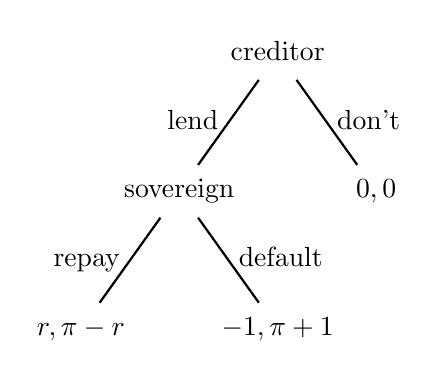
\begin{tikzpicture}[
			edge from parent/.style={thick, draw, font=\normalsize},
			decision/.style={font=\normalsize},
			terminal/.style={font=\normalsize},
			sibling distance=2.5cm,
			level distance=1.75cm
			]
			\node[decision] (creditor) {creditor\strut}
				child { node[decision] (sovereign) {sovereign\strut}
					child { node[terminal] {$r,\pi - r$\strut} edge from parent node[midway, left] {repay\strut} }
					child { node[terminal] {$-1,\pi + 1$\strut} edge from parent node[midway, right] {default\strut} }
					edge from parent node[midway, left] {lend\strut}
					}
				child { node[terminal] {$0,0$\strut} edge from parent node[midway, right] {don't\strut} };
		\end{tikzpicture}
		\caption{The stage game in \Cref{example:sovereign}.}
		\label{fig:sov}
	\end{figure}
	%
	Formally, this is the public-monitoring stage game $G = \left( I, Y, (A_i, u_i)_{i \in I}, \mu \right)$ with players $I \coloneqq \{\text{c(reditor)},\text{s(overeign)}\}$, actions $A_{\text{c}} \coloneqq \{\text{lend},\text{don't}\}$ and $A_{\text{s}} \coloneqq \{\text{repay},\text{default}\}$, monitoring structure $(Y,\mu)$ where $Y \coloneqq \text\{ \text{don't}, (\text{lend},\text{repay}), (\text{lend},\text{default}) \}$ and 
	%
	\begin{align*}
		\mu(\text{don't}|(\text{don't},\text{repay}))
		&\coloneqq 1 ,
		\\
		\mu(\text{don't}|(\text{don't},\text{default}))
		&\coloneqq 1 ,
		\\
		\mu((\text{lend},\text{repay})|(\text{lend},\text{repay}))
		&\coloneqq 1
		\quad \text{and}
		\\
		\mu((\text{lend},\text{default})|(\text{lend},\text{default}))
		&\coloneqq 1 ,
	\end{align*}
	%
	and payoffs
	%
	\begin{equation*}
		\left( u_{\text{c}}(a_{\text{c}},y) ,
		u_{\text{s}}(a_{\text{s}},y) \right)
		\coloneqq
		\begin{cases}
			(0,0) & \text{if $y = \text{don't}$} \\
			(r,\pi - r) & \text{if $y = (\text{lend},\text{repay})$} \\
			(-1,\pi + 1) & \text{if $y = (\text{lend},\text{default})$.}
		\end{cases}
	\end{equation*}

	Evidently the unique subgame-perfect equilibrium of the stage game $G$ is $(\text{don't},\text{default})$, which is Pareto-dominated by the strategy profile $(\text{lend},\text{repay})$ since $\pi > r > 0$. Are there equilibria of the \emph{repeated} game $(G,\delta)$ in which $(\text{lend},\text{repay})$ is played in every period on the path? (Yes if $\delta \geq (1+r)/(1+\pi)$, as we shall show in \cref{aps:examples:sovereign_gen} below.)
	%
\end{example}

What makes public monitoring `public' is that it is always commonly known what players know about other players' past actions: everyone observes $y \in Y$ and nothing else, everyone knows that everyone observes $y \in Y$ and nothing else, everyone knows that everyone knows that everyone observes $y \in Y$ and nothing else, and so on. This `publicness' property is built in to the definition of a public-monitoring repeated game. One can consider a more general type of repeated game in which players may observe \emph{private} signals which are informative about other players' past actions; these are called \emph{private-monitoring repeated games.} An example is if player~1 \emph{privately} observes the realisation of a noisy signal that is informative about player~2's last action, so that player~2 and player~3 do not know what player~1 knows (or believes) about player~2's last action. Private monitoring is arguably natural in many economic applications, but it is much less tractable than the public-monitoring case, and thus beyond the scope of this chapter. See \textcite[][chapters~12--14]{MailathSamuelson2006} if you're curious.

The definitions above of public-monitoring stage and repeated games omit some measure-theoretic niceties. We will sweep all such unpleasantness under the rug by focussing on \emph{finite} games. A public-monitoring stage game $G = \left( I, Y, (A_i, u_i)_{i \in I}, \mu \right)$ is called \emph{finite} iff the sets $I$, $Y$ and $(A_i)_{i \in I}$ are all finite. A public-monitoring repeated game $(G,\delta)$ is called \emph{finite} iff the public-monitoring stage game $G$ is finite. Our focus on finite games is for simplicity only; all of the results in this chapter do extend to infinite games \parencite[see][chapter~7]{MailathSamuelson2006}.

\begin{remark}
	%
	\label{remark:rep_game_formal}
	%
	As mentioned above, for a finite public-information stage game $G = \left( I, Y, (A_i, u_i)_{i \in I}, \mu \right)$ and a $\delta \in (0,1)$, the public-monitoring repeated game $(G,\delta)$ is formally an extensive-form game, namely
	%
	\begin{equation*}
		\left(\widetilde{I},\widetilde{\mathcal{A}},\widetilde{H},\widetilde{P},\widetilde{\mathcal{S}},\left(\widetilde{u}_i\right)_{i \in I},\widetilde{\pi}\right)
	\end{equation*}
	%
	where
	%
	\begin{itemize}
	
		\item the players are $\widetilde{I} \coloneqq I$,
		
		\item the actions are $\widetilde{\mathcal{A}} \coloneqq \left( \bigcup_{i \in I} A_i \right) \cup Y$,

		\item the histories $\widetilde{H}$ are all sequences $h$ in $\widetilde{\mathcal{A}}$ (including the empty sequence) such that for each $k \in \N$, the $k^\text{th}$ entry of $h$

		\begin{itemize}
		
			\item belongs to $A_1$ if $k = (\abs*{I}+1) n + 1$ for some $n \in \{0,1,2,3,\dots\}$,

			\item belongs to $A_2$ if $k = (\abs*{I}+1) n + 2$ for some $n \in \{0,1,2,3,\dots\}$,

			\item[\vdots]

			\item belongs to $A_{\abs*{I}}$ if $k = (\abs*{I}+1) n + \abs*{I}$ for some $n \in \{0,1,2,3,\dots\}$, and

			\item belongs to $Y$ if $k = (\abs*{I}+1) (n+1)$ for some $n \in \{0,1,2,3,\dots\}$,
		
		\end{itemize}
		%
		(where the non-terminal histories are the finite ones, and the terminal histories are the infinite ones,)

		\item the action and player functions $\widetilde{A}$ and $\widetilde{P}$ are given by

		\begin{itemize}
		
			\item $\widetilde{A}(h) \coloneqq A_1$ and $\widetilde{P}(h) \coloneqq 1$ if $\text{length}(h) = (\abs*{I}+1) n$ for some $n \in \{0,1,2,3,\dots\}$,
		
			\item $\widetilde{A}(h) \coloneqq A_2$ and $\widetilde{P}(h) \coloneqq 2$ if $\text{length}(h) = (\abs*{I}+1) n + 1$ for some $n \in \{0,1,2,3,\dots\}$,

			\item[\vdots]

			\item $\widetilde{A}(h) \coloneqq A_{\abs*{I}}$ and $\widetilde{P}(h) \coloneqq \abs*{I}$ if $\text{length}(h) = (\abs*{I}+1) n + \abs*{I}-1$ for some $n \in \{0,1,2,3,\dots\}$, and

			\item $\widetilde{A}(h) \coloneqq Y$ and $\widetilde{P}(h) \coloneqq \text{Nature}$ if $\text{length}(h) = (\abs*{I}+1) n + \abs*{I}$ for some $n \in \{0,1,2,3,\dots\}$,
		
		\end{itemize}

		\item the information sets $\widetilde{\mathcal{S}}$ are, for each non-terminal (meaning \emph{finite}) history $h \in \widetilde{H}$,

		\begin{itemize}
		
			\item if $\widetilde{P}(h) = i \in I$, then the information set $\widetilde{\mathcal{S}}(h)$ comprises all non-terminal histories $h'$ such for every $n \in \{0,1,2,3,\dots\}$, the $[(\abs*{I}+1) n + i]^\text{th}$ and $[(\abs*{I}+1) (n+1)]^\text{th}$ entries of $h$ and $h'$ (if there are such entries) are equal, and

			\item if $\widetilde{P}(h) = \text{Nature}$, then $\widetilde{\mathcal{S}}(h) \coloneqq \{h\}$,
		
		\end{itemize}

		\item the payoff functions $\left(\widetilde{u}_i\right)_{i \in I}$ are given by, for each terminal (meaning \emph{infinite}) history
		%
		\begin{equation*}
			h = \left(a_1^1,a_2^1,\dots,a_{\abs*{I}}^1,y^1,a_1^2,a_2^2,\dots,a_{\abs*{I}}^2,y^2,a_1^3,a_2^3,\dots,a_{\abs*{I}}^3,y^3,\dots\right) \in \widetilde{H} ,
		\end{equation*}
		%
		and each player $i \in I$,
		%
		\begin{equation*}
			\widetilde{u}_i(h) \coloneqq (1-\delta) \sum_{t=0}^\infty \delta^t u_i(a_i^t,y^t) ,
		\end{equation*}
		%
		and

		\item the Nature strategy function $\widetilde{\pi}$ is given by, for each non-terminal (meaning \emph{finite}) history
		%
		\begin{multline*}
			h = \Bigl(
			a_1^1,a_2^1,\dots,a_{\abs*{I}}^1,y^1,
			a_1^2,a_2^2,\dots,a_{\abs*{I}}^2,y^2,\dots,\\
			a_1^{t-1},a_2^{t-1},\dots,a_{\abs*{I}}^{t-1},y^{t-1},
			a_1^t,a_2^t,\dots,a_{\abs*{I}}^t\Bigr) \in \widetilde{H} 
		\end{multline*}
		%
		such that $\widetilde{P}(h)=\text{Nature}$,
		%
		\begin{equation*}
			\widetilde{\pi}(h) \coloneqq \mu\left(\cdot\middle|a_1^t,a_2^t,\dots,a_{\abs*{I}}^t\right) \in \Delta(Y) .
		\end{equation*}

	\end{itemize}
	%
\end{remark}




%%%%%%%%%%%%%%%%%%%%%%%%%%%%%%%%%%%
%%%%%%%%%%%%%%%%%%%%%%%%%%%%%%%%%%%
\section{Histories, strategies, payoffs}
\label{aps:hist}
%%%%%%%%%%%%%%%%%%%%%%%%%%%%%%%%%%%
%%%%%%%%%%%%%%%%%%%%%%%%%%%%%%%%%%%

For any non-empty set $X$ and $t \in \N$, recall that $X^t$ denotes the set of length-$t$ sequences in $X$, i.e.
%
\begin{equation*}
	X^t
	\coloneqq \left\{ \left( x^0, x^1, x^2, \dots, x^{t-1} \right) : x^0 \in X,\, x^1 \in X,\, x^2 \in X, \dots,\, x^{t-1} \in X \right\} .
\end{equation*}
%
There is of course only one length-$0$ sequence in $X$, namely the empty sequence, which we denote by $\varnothing$; for this reason, we write $X^0 \coloneqq \{\varnothing\}$.

Fix a finite public-monitoring repeated game
%
\begin{equation*}
	(G,\delta) = \left( I, Y, (A_i, u_i)_{i \in I}, \mu, \delta \right) .
\end{equation*}
%
At the start of each period $t \in \{0,1,2,3,\dots\}$, there is a \emph{public history}
%
\begin{equation*}
	h^{t-1} \equiv \left(y^0,y^1,y^2,\dots,y^{t-1}\right) \in Y^t
\end{equation*}
%
observed by all players and, for each player $i \in I$, a \emph{private history}
%
\begin{equation*}
	h^{t-1}_i \equiv \left(y^0,a^0_i,y^1,a^1_i,y^2,a^2_i,\dots,y^{t-1},a^{t-1}_i\right) \in (Y \times A_i)^t
\end{equation*}
%
observed only by player~$i$.

A \emph{(behavioural) strategy} of player $i \in I$ is a map $\sigma_i : \Union_{t=0}^\infty (Y \times A_i)^t \to \Delta(A_i)$ which specifies a (mixed) action at each private history of player~$i$. A (behavioural) strategy $\sigma_i$ of player $i \in I$ is called \emph{public} iff it is measurable with respect to the public history, i.e. there exists a function $\tau_i : \Union_{t=0}^\infty Y^t \to \Delta(A_i)$ such that
%
\begin{equation*}
	\sigma_i\left(y^0,a^0_i,y^1,a^1_i,y^2,a^2_i,\dots,y^{t-1},a^{t-1}_i\right)
	= \tau_i\left( y^0, y^1, y^2, \dots, y^{t-1} \right)
\end{equation*}
%
for every private history
%
\begin{equation*}
	\left(y^0,a^0_i,y^1,a^1_i,y^2,a^2_i,\dots,y^{t-1},a^{t-1}_i\right)
	\in (Y \times A_i)^t .
\end{equation*}
%
A \emph{(public) strategy profile} is a collection $\sigma = (\sigma_i)_{i \in I}$ of (public) strategies, one for each player. For a public strategy profile $\sigma$, we abuse notation by writing $\sigma\bigl(h^{t-1}\bigr) \in \prod_{i \in I} \Delta(A_i)$ for the profile of mixed actions played at public history $h^{t-1} \in Y^t$. (Why is this an abuse of notation?)

Any public strategy profile $\sigma$ generates, for each $t \in \{0,1,2,3,\dots\}$, a random length-$t$ public history $h^{t-1}_\sigma \in Y^t$: in particular, $h^{-1}_\sigma \coloneqq \varnothing$ (the empty sequence), $h^0_\sigma \coloneqq (y^0_\sigma)$ where $y^0_\sigma$ is drawn from $\mu\left( \cdot \middle| \sigma\left( h^{-1}_\sigma \right) \right)$, $h^1_\sigma \coloneqq \left(h^0_\sigma,y^1_\sigma\right)$ where $y^1_\sigma$ is drawn from $\mu\left( \cdot \middle| \sigma\left( h^0_\sigma \right) \right)$, $h^2_\sigma \coloneqq \left(h^1_\sigma,y^2_\sigma\right)$ where $y^2_\sigma$ is drawn from $\mu\left( \cdot \middle| \sigma\left( h^1_\sigma \right) \right)$, and so on, where the draws are jointly independent. The lifetime expected payoff of player $i \in I$ from the strategy profile $\sigma$ is denoted
%
\begin{equation*}
	U_i(\sigma) \coloneqq \E\left( (1-\delta) \sum_{t=0}^\infty \delta^t u_i\left( \sigma\left(h^{t-1}_\sigma\right) \right) \right) .
\end{equation*}
%
We write $U(\sigma) \coloneqq (U_i(\sigma))_{i \in I}$ for the vector of all players' lifetime expected payoffs. Similarly, we write $u(\alpha) \coloneqq (u_i(\alpha))_{i \in I}$ for the vector of all players' stage-game payoffs from a profile $\alpha \in \prod_{i \in I} \Delta(A_i)$ of mixed actions.

Although the `continuation game' starting from a public history $h^{t-1} \in Y^t$ is \emph{not} a subgame (except if monitoring is perfect), it can still be treated as a game in its own right \emph{provided} players play a public strategy profile, since then players' private information about their own past play is irrelevant for payoffs going forward. By inspection, this `continuation game' is identical with the full public-monitoring repeated game $(G,\delta)$ itself: the game is $G$ is played repeatedly, with public outcomes drawn conditionally independently over time, and payoffs discounted by $\delta$.

Given a public strategy profile $\sigma$ and a public history $h_{*}^{t-1} \in Y^t$, the \emph{continuation strategy profile} is the strategy profile $\sigma|_{h_{*}^{t-1}}$ defined by
%
\begin{equation*}
	\left.\sigma\right|_{h_{*}^{t-1}}\left( h^{s-1} \right)
	\coloneqq \sigma\left( h_{*}^{t-1}, h^{s-1} \right)
	\quad \text{for each public history $h^{s-1} \in Y^s$.}
\end{equation*}
%
To be very clear about notation here: $(h_{*}^{t-1}, h^{s-1}) \in Y^{t+s}$ is the sequence in $Y$ obtained by concatenating the sequences $h_{*}^{t-1} \in Y^t$ and $h^{s-1} \in Y^s$. In other words, $(h_{*}^{t-1}, h^{s-1})$ is the length-$(t+s)$ public history in which public outcomes are $h_{*}^{t-1}$ in periods $\{0,1,2,3,\dots,t-2,t-1\}$ and $h^{s-1}$ in periods $\{t,t+1,t+2,t+3,\dots,t+s-2,t+s-1\}$.

Obviously every continuation of a public strategy profile is itself public. For each player $i \in I$, we write $\sigma_i|_{h^{t-1}} \coloneqq \left( \sigma|_{h^{t-1}} \right)_i$ for $i$'s continuation strategy and $\sigma_{-i}|_{h^{t-1}} \coloneqq \left( \sigma|_{h^{t-1}} \right)_{-i}$ for the profile of continuation strategies of her opponents.

The \emph{continuation payoff} of a public strategy profile $\sigma$ at a public history $h_{*}^{t-1} \in Y^t$ is the payoff from play of the (public) continuation strategy profile $\sigma_{*} \coloneqq \sigma|_{h_{*}^{t-1}}$ in the `continuation game' that starts at $h_{*}^{t-1}$, i.e.
%
\begin{align*}
	U\left( \sigma_{*} \right)
	&= \E\left( (1-\delta) \sum_{s=0}^\infty \delta^s u\left( \sigma_{*}\left(h^{s-1}_{\sigma_{*}}\right) \right) \right)
	\\
	&= \E\left( (1-\delta) \sum_{s=t}^\infty \delta^{s-t} u\left( \sigma\left(h_{*}^{t-1},h^{s-t-1}_{\sigma_{*}} \right) \right) \right) .
\end{align*}
%
Note that by definition, the continuation payoff from public history $h_{*}^{t-1} \in Y^t$ omits per-period payoffs enjoyed in periods $\{0,1,2,3,\dots,t-1\}$; it is a forward-looking object.

Continuation payoffs of public strategy profiles have a recursive structure: for any public strategy profile $\sigma$ and public history $h^{t-1} \in Y^t$,
%
\begin{equation*}
	U\left(\sigma|_{h^{t-1}}\right)
	= (1-\delta) u\left( \sigma\left( h^{t-1} \right) \right)
	+ \delta \E\left( U\left( \sigma|_{\left( h^{t-1}, y^t \right)} \right) \right),
\end{equation*}
%
where $y^t$ is a random draw from the distribution $\mu\left( \cdot \middle| \sigma\left( h^{t-1} \right) \right)$; in other words,
%
\begin{equation*}
	U\left(\sigma|_{h^{t-1}}\right)
	= (1-\delta) u\left( \sigma\left( h^{t-1} \right) \right)
	+ \delta \sum_{y \in Y}
	U\left( \sigma|_{\left( h^{t-1}, y \right)} \right)
	\mu\left( y \middle| \sigma\left( h^{t-1} \right) \right) .
\end{equation*}



%%%%%%%%%%%%%%%%%%%%%%%%%%%%%%%%%%%
%%%%%%%%%%%%%%%%%%%%%%%%%%%%%%%%%%%
\section{Perfect public equilibrium}
\label{aps:ppe}
%%%%%%%%%%%%%%%%%%%%%%%%%%%%%%%%%%%
%%%%%%%%%%%%%%%%%%%%%%%%%%%%%%%%%%%

Again fix a finite public-monitoring repeated game
%
\begin{equation*}
	(G,\delta) = \left( I, Y, (A_i, u_i)_{i \in I}, \mu, \delta \right) .
\end{equation*}
%
A player~$i$ may sometimes strictly prefer a non-public strategy over all public strategies. In particular, if ($i$ believes that) a player $j \neq i$ is playing a non-public strategy, then player~$j$'s actions today depend on what actions she took in the past, which only she knows. To predict player~$j$'s choice of action, player~$i$ must guess player~$j$'s past actions based on past public outcomes. The distribution of these outcomes depend both on her own past actions and on those of player~$j$. Thus to draw correct inferences about what actions player~$j$ likely took in the past, player~$i$ must in general make use of her knowledge of her \emph{own} past actions. When choosing her action based on a belief formed in this way, player~$i$'s action may well depend on what actions she herself took in previous periods. In other words, she may wish to use a non-public strategy.

However, if (player~$i$ believes that) the other players play \emph{public} strategies, then she always has a public best reply:

\begin{observation}
	%
	\label{observation:public_br}
	%
	Fix a finite public-monitoring repeated game
	%
	\begin{equation*}
		(G,\delta) = \left( I, Y, (A_i, u_i)_{i \in I}, \mu, \delta \right) ,
	\end{equation*}
	%
	a player $i \in I$, a public history $h^{t-1} \in Y^t$, and strategies $\sigma_j : \Union_{t=0}^\infty (Y \times A_j)^t \to \Delta(A_j)$ of each other player $j \in I \setminus \{i\}$. If $\sigma_j$ is public for each $j \in I \setminus \{i\}$, then $i$ has a public best reply at $h^{t-1}$: that is, there is a public strategy $\sigma_i$ of player~$i$ such that
	%
	\begin{equation*}
		U_i\left( \sigma|_{h^{t-1}} \right) \geq U_i\left( \sigma_i', \sigma_{-i}|_{h^{t-1}} \right)
	\end{equation*}
	%
	for every strategy $\sigma_i'$ of player~$i$.
	%
\end{observation}

This is (nearly) obvious upon reflection: player~$i$'s past actions are not directly payoff-relevant in the `continuation game' starting at $h^{t-1}$, so they matter for her choice of action only insofar as they are informative about something that \emph{is} payoff-relevant, viz. other players' actions; but they aren't, since the other players play public strategies.

\begin{definition}
	%
	\label{definition:ppe}
	%
	A public strategy profile $\sigma = (\sigma_i)_{i \in I}$ is a \emph{perfect public equilibrium} (`PPE' for short) of $(G,\delta)$ iff for every public history $h^{t-1} \in Y^t$,
	%
	\begin{equation*}
		U_i\left( \sigma|_{h^{t-1}} \right)
		\geq U_i\left( \sigma_i', \sigma_{-i}|_{h^{t-1}} \right)
	\end{equation*}
	%
	for every player $i \in I$ and each strategy $\sigma_i'$ of player~$i$.
	%
\end{definition}

In other words, in every `continuation game' (formally, at each public history $h^{t-1} \in Y^t$), for each player $i \in I$, her continuation strategy $\sigma_i|_{h^{t-1}}$ is a best reply: she cannot improve her (expected) continuation payoff by deviating to another strategy $\sigma'$. PPE is in the spirit of subgame-perfect equilibrium, but the two formally coincide only if monitoring is perfect, since otherwise `continuation games' are not true subgames. PPE is a refinement of perfect Bayesian equilibrium.

Note that we quantify over \emph{all} alternative strategies $\sigma_i'$ of player~$i$, not only public strategies. By \Cref{observation:public_br} above, it would make no difference if we were to quantify only over \emph{public} strategies $\sigma_i'$.

\begin{observation}
	%
	\label{observation:ppe_conts}
	%
	A public strategy profile $\sigma$ is a PPE if and only if for every public history $h^{t-1} \in Y^t$, the continuation strategy profile $\sigma|_{h^{t-1}}$ is a PPE.
	%
\end{observation}

When the solution concept is PPE, every finite public-monitoring repeated game satisfies the one-shot deviation principle:

\begin{proposition}
	%
	\label{proposition:ppe_osdp}
	%
	Fix a finite public-monitoring repeated game
	%
	\begin{equation*}
		(G,\delta) = \left( I, Y, (A_i, u_i)_{i \in I}, \mu, \delta \right) .
	\end{equation*}
	%
	A public strategy profile $\sigma$ is a PPE iff for every public history $h^{t-1} \in Y^t$, every player $i \in I$ and each action $a_i \in A_i$,
	%
	\begin{equation*}
		U_i\left( \sigma|_{h^{t-1}} \right)
		\geq (1-\delta) u_i\left( a_i, \sigma_{-i}\left( h^{t-1} \right) \right)
		+ \delta \E\left( U_i\left( \sigma|_{\left(h^{t-1},y^t\right)} \right) \right) ,
	\end{equation*}
	%
	where $y^t$ is a random draw from the distribution $\mu\left( \cdot \middle| a_i, \sigma_{-i}\left( h^{t-1} \right) \right)$.
	%
\end{proposition}

In other words, there is no public history $h^{t-1} \in Y^t$ at which a player $i \in I$ strictly gains by playing $a_i \neq \sigma_i\left( h^{t-1} \right)$ and then reverting to follow the strategy $\sigma_i$ in all subsequent periods.

\Cref{proposition:ppe_osdp} can be reformulated in language closer to that of the \hyperref[ch_osdp]{previous chapter}, as follows. For public strategies $\sigma_i$ and $\sigma_i'$ of a player $i \in I$, we say that $\sigma_i'$ is a \emph{one-shot deviation} from $\sigma_i$ iff $\sigma_i\left( h^{t-1} \right) \neq \sigma_i'\left( h^{t-1} \right)$ for exactly one public history $h^{t-1} \in Y^t$. \Cref{proposition:ppe_osdp} says precisely that a public strategy profile $\sigma$ is a PPE iff for every player $i \in I$ and every one-shot deviation $\sigma_i'$ from $\sigma_i$, letting $h^{t-1} \in Y^t$ be the (unique) public history at which $\sigma_i\left( h^{t-1} \right) \neq \sigma_i'\left( h^{t-1} \right)$, it holds that
%
\begin{equation*}
	U_i\left( \sigma|_{h^{t-1}} \right)
	\geq U_i\left( \sigma_i', \sigma_{-i}|_{h^{t-1}} \right) .
\end{equation*}

\begin{exercise}
	%
	\label{exercise:osdp_ppe}
	%
	Prove \Cref{proposition:ppe_osdp}. (Hint: learn from the \hyperref[ch_osdp]{previous chapter}.)
	%
\end{exercise}



%%%%%%%%%%%%%%%%%%%%%%%%%%%%%%%%%%%
%%%%%%%%%%%%%%%%%%%%%%%%%%%%%%%%%%%
\section{Feasible payoffs}
\label{aps:feasible}
%%%%%%%%%%%%%%%%%%%%%%%%%%%%%%%%%%%
%%%%%%%%%%%%%%%%%%%%%%%%%%%%%%%%%%%

Again fix a finite public-monitoring repeated game
%
\begin{equation*}
	(G,\delta) = \left( I, Y, (A_i, u_i)_{i \in I}, \mu, \delta \right) .
\end{equation*}
%
Let $X \subseteq \R^{\abs*{I}}$ be the the convex hull of $\left\{ u(a) : a \in A \right\}$. Equivalently,
%
\begin{equation*}
	X \coloneqq \left\{
	u(\alpha) : \alpha \in \Delta(A)
	\right\} .
\end{equation*}
%
Note that we quantify over all mixed action profiles $\alpha \in \Delta(A)$, including those that feature correlation between different players' actions; we do \emph{not} restrict attention to independent-mixing profiles $\alpha \in \prod_{i \in I} \Delta(A_i)$.

Obviously $u(\alpha) \in X$ for any mixed action profile $\alpha \in \Delta(A)$. It follows that $U(\sigma) \in X$ for any strategy profile $\sigma$. (Make sure that you understand why.) 

\begin{remark}
	%
	\label{remark:X_converse}
	%
	It is not true in general that \emph{every} $v \in X$ can be obtained from play either of the stage game $G$ or of the repeated game $(G,\delta)$. For example, let $G$ be the public-monitoring stage game formed by adding public monitoring to \Cref{example:BoS} (\cref{ch_dom}, \cpageref{example:BoS}). Assume that $\eps>0$. $X$ equals the convex hull of $\{ (0,0), (1,1+\eps), (1+\eps,1) \}$. Consider the payoff vector $v = \left( 1+\eps/2, 1+\eps/2 \right) \in X$.

	\begin{enumerate}[label=(\alph*)]
	
		\item \label{item:X_converse:stage} In the stage game $G$, if players cannot correlate their actions (i.e. they must mix independently, the usual assumption in game theory), then $v$ is unattainable: formally, there is no $\alpha = (\alpha_1,\alpha_2) \in \Delta(A_1) \times \Delta(A_2)$ such that $u(\alpha) = v$.

		\begin{exercise}
			%
			\label{exercise:X_converse:stage}
			%
			Prove it!
			%
		\end{exercise}

		\item \label{item:X_converse:rep} In the repeated game $(G,\delta)$, if $\delta \in (0,1)$ is small enough, then $v$ is unattainable: formally, there is no strategy profile $\sigma$ such that $U(\sigma)=v$.

		\begin{exercise}
			%
			\label{exercise:X_converse:rep}
			%
			Prove it! (Hint: consider $\delta=0$, and recall claim \ref{item:X_converse:stage}.)
			%
		\end{exercise}
	
	\end{enumerate}

	However, there are assumptions under which for an arbitrary public-monitoring stage game $G$, every $v \in X$ is attainable in $G$ and/or $(G,\delta)$.

	\begin{enumerate}[label=(\alph*),resume]

		\item \label{item:X_converse:stage_pos} Obviously every payoff vector in $X$ can be attained by play of the \emph{stage} game $G$ provided players can somehow correlate their action choices. This can be achieved using a \emph{public correlating device,} meaning a payoff-irrelevant random variable whose realisation becomes known before players choose their actions; by conditioning their action choices on the realisation of this random variable, players can achieve correlation between their actions.
		(Such public correlating devices are also the conceptual scaffolding of correlated equilibrium.) To be able to achieve \emph{every} $v \in X$, it is necessary for the public correlating device to be sufficiently rich; the usual assumption is that it has full support on a continuum (for example, a Uniformly distributed random variable).%
			\footnote{If players can communicate before choosing their actions, then correlation can be achieved without a public correlating device by using a communication scheme called a \emph{jointly controlled lottery.} See \textcite[][p.~18]{MailathSamuelson2006}.}

		\item \label{item:X_converse:rep_pos} If the discount factor $\delta \in (0,1)$ is large enough, then every payoff in $X$ can be attained by play of the \emph{repeated} game $(G,\delta)$: that is, for each $v \in X$, there is a strategy profile $\sigma$ such that $U(\sigma) = v$. The idea is to replace randomisation with alternation: for any $\alpha \in \Delta(A)$, instead of drawing an action profile once and for all from $\supp \alpha$ (with probability weights $\alpha \in \Delta(A)$), we alternate over time between action profiles in $\supp \alpha$ (with time shares determined by $\alpha$ and $\delta$).

		To illustrate the idea, consider again \Cref{example:BoS} with perfect monitoring. If $\delta=1/2$, then the payoff vector $v = \left( 1+\eps/2, 1+\eps/2 \right) \in X$ is attainable: in particular, $U(\sigma)=v$ for the (pure) strategy profile $\sigma$ that plays $(B,B)$ in period $t=0$ and $(S,S)$ in every subsequent period.

	\end{enumerate}
	%
\end{remark}



%%%%%%%%%%%%%%%%%%%%%%%%%%%%%%%%%%%
%%%%%%%%%%%%%%%%%%%%%%%%%%%%%%%%%%%
\section{APS}
\label{aps:selfgen}
%%%%%%%%%%%%%%%%%%%%%%%%%%%%%%%%%%%
%%%%%%%%%%%%%%%%%%%%%%%%%%%%%%%%%%%

Again fix a finite public-monitoring repeated game
%
\begin{equation*}
	(G,\delta) = \left( I, Y, (A_i, u_i)_{i \in I}, \mu, \delta \right) .
\end{equation*}
%
We are interested in the PPE payoff set
%
\begin{equation*}
	E \coloneqq 
	\left\{
	U(\sigma) : \text{$\sigma$ is a PPE}
	\right\}
	\subseteq X .
\end{equation*}

One thing which you may already (kind of) know about $E$ is that provided $G$ satisfies some arguably weak conditions,%
	\footnote{The key one is that ($\mu$ is such that) actions are identified (in the econometric sense) off public outcomes.}
then as $\delta$ approaches $1$, the set $E$ grows very large: it eventually includes every payoff vector $v \in X$ that lies in the interior of $X$ and is strictly individually rational in the sense that
%
\begin{equation*}
	v_i > \min_{\alpha_{-i} \in \Delta(A_{-i})} \max_{a_i \in A_i} u_i(a_i,\alpha_{-i})
	\quad \text{for every player $i \in I$.}
\end{equation*}
%
This the folk theorem of \textcite{FudenbergLevineMaskin1994} \parencite[see][chapter~9]{MailathSamuelson2006}.

It is important to understand that the folk theorem tells us nothing at all about the PPE payoffs (or equilibria) of a given public-monitoring repeated game $(G,\delta)$ arising in an economic application. What it tells us is, rather, that for every strictly individually rational payoff vector $v \in \interior X$, there is some \emph{other} public-monitoring repeated game $(G',\delta')$ in which $v$ is a PPE payoff, and furthermore $(G',\delta')$ may be chosen so that $G'=G$.

The technique developed in this section, called `APS' after \textcite{AbreuPearceStacchetti1990}, instead characterises the PPE payoff set $E$ of a \emph{given} game $(G,\delta)$ (jargon: `a characterisation at fixed discounting'). It is a dynamic-programming-like characterisation. In particular, it is rooted in the two recursive properties of PPEs from the previous section: the fact that a PPE has only PPE continuations (\Cref{observation:ppe_conts}) and the one-shot deviation principle (\Cref{proposition:ppe_osdp}). The former property implies that if $\sigma$ is a PPE, then $U\left( \sigma|_{h^{t-1}} \right) \in E$ for every public history $h^{t-1} \in Y^t$. The latter property implies the following `converse':

\begin{corollary}
	%
	\label{corollary:enforcement}
	%
	Fix a map $\beta : Y \to E$ and a profile $\alpha \in \prod_{i \in I} \Delta(A_i)$ of mixed actions, and let
	%
	\begin{equation*}
		v \coloneqq (1-\delta) u(\alpha) + \delta \sum_{y \in Y} \beta(y) \mu(y|\alpha) .
	\end{equation*}
	%
	If
	%
	\begin{equation}
		v_i \geq (1-\delta) u_i(a_i,\alpha_{-i}) + \delta \sum_{y \in Y} \beta_i(y) \mu(y|a_i,\alpha_{-i})
		\label{eq:enforcement_cor}
	\end{equation}
	%
	for each player $i \in I$ and action $a_i \in A_i$, then $v \in E$.
	%
\end{corollary}

\begin{proof}
	%
	For each $y \in Y$, since $\beta(y) \in E$, there is a PPE $\sigma_y$ such that $U(\sigma_y) = \beta(y)$. Define a strategy profile $\sigma$ by $\sigma(\varnothing) \coloneqq \alpha$ and $\sigma|_{\left(y^0\right)} \coloneqq \sigma_{y^0}$ for each $y^0 \in Y$. Since \eqref{eq:enforcement_cor} holds for each player $i \in I$ and action $a_i \in A_i$, no player has a strictly profitable one-shot deviation at the initial public history $\varnothing$. Since $\sigma|_{\left(y^0\right)} = \sigma_{y^0}$ is a PPE for each $y^0 \in Y$, no player has a strictly profitable deviation at any public history besides $\varnothing$. Hence by the one-shot deviation principle (\Cref{proposition:ppe_osdp}), $\sigma$ is a PPE. Obviously $U(\sigma)=v$.
	%
\end{proof}

\Cref{corollary:enforcement} suggests an analogy with (multi-agent) moral hazard, where agents' actions are not directly observable, but (randomly) generate a public outcome (`output') which is contractible. By designing an \emph{incentive scheme,} which specifies rewards as a function of the public outcome, agents can be incentivised to take some actions rather than others.

The map $\beta : Y \to E$ in \Cref{corollary:enforcement} is an incentive scheme in this sense: the inequalities \eqref{eq:enforcement_cor} are incentive-compatibility constraints, which say that players are willing to play $\alpha$. The key difference with moral hazard is that rewards $\beta(y)$ are delivered not in cash, but rather in the form of \emph{continuation values} generated by future play.

In order for players to be willing actually to follow through with this future play, it must be a PPE; this constraint is of course absent when incentives are provided using cash (assuming remuneration is agreed in a legally enforceable contract). In \Cref{corollary:enforcement}, this constraint is satisfied because of the assumption that $\beta(y) \in E$ for each $y \in Y$; this means (by definition of $E$) that for each $y \in Y$, there is a PPE $\sigma_y$ which delivers the continuation value $U(\sigma_y) = \beta(y)$.

\Cref{corollary:enforcement} will be the inspiration for our recursive characterisation of $E$. We will use the following terminology.

\begin{definition}
	%
	\label{definition:enforcement}
	%
	A map $\beta : Y \to X$ \emph{enforces} a profile $\alpha \in \prod_{i \in I} \Delta(A_i)$ of mixed actions iff
	%
	\begin{align*}
		(1-\delta) u_i(\alpha) &+ \delta \sum_{y \in Y} \beta_i(y) \mu(y|\alpha)
		\\
		\geq (1-\delta) u_i(a_i,\alpha_{-i}) &+ \delta \sum_{y \in Y} \beta_i(y) \mu(y|a_i,\alpha_{-i})
	\end{align*}
	%
	for each player $i \in I$ and action $a_i \in A_i$.
	%
\end{definition}

Enforcement captures incentive-compatibility. In the language of moral hazard, we would say that $\beta$ \emph{implements} $\alpha$.

\begin{remark}
	%
	\label{remark:enforc_nash}
	%
	An equivalent definition is that $\beta : Y \to X$ enforces $\alpha \in \prod_{i \in I} \Delta(A_i)$ iff $\alpha$ is a Nash equilibrium of the (artificial, static) normal-form game $\left(I,(A_i,w_i\right)_{i \in I})$, where for each player $i \in I$, the (artificial) payoff $w_i : A \to \R$ is given by
	%
	\begin{equation*}
		w_i(a) \coloneqq (1-\delta) u_i(a) + \delta \sum_{y \in Y} \beta_i(y) \mu(y|a)
		\quad \text{for each action profile $a \in A$.}
	\end{equation*}
	%
\end{remark}

\begin{definition}
	%
	\label{definition:generation}
	%
	A set $V \subseteq X$ of payoff vectors \emph{generates} a payoff vector $v \in X$ iff there exists a map $\beta : Y \to V$ and a profile $\alpha \in \prod_{i \in I} \Delta(A_i)$ of mixed actions such that $\beta$ enforces $\alpha$ and
	%
	\begin{equation*}
		(1-\delta) u(\alpha)
		+ \delta \sum_{y \in Y} \beta(y) \mu(y|\alpha) 
		= v.
	\end{equation*}
	%
\end{definition}

What it means for $v \in X$ to be generated by $V \subseteq X$ is simply that it is possible, using only rewards in $V$, to design an incentive scheme (a map $\beta : Y \to V$) under which (actions $\alpha \in \prod_{i \in I} \Delta(A_i)$ are chosen such that) payoffs are precisely $v$.

\begin{definition}
	%
	\label{definition:gen_B}
	%
	The \emph{generating function (or `APS operator')} is the map $B : 2^X \to 2^X$ defined by $B(V) \coloneqq \left\{ v \in X : \text{$v$ is generated by $V$} \right\}$ for each $V \subseteq X$.
	%
\end{definition}

\begin{proposition}
	%
	\label{proposition:self-gen}
	%
	In a finite public-monitoring repeated game, if a set $V \subseteq X$ satisfies $V \subseteq B(V)$, then it is contained in the PPE payoff set, i.e. $V \subseteq E$.
	%
\end{proposition}

A set $V \subseteq X$ such that $V \subseteq B(V)$ is called \emph{self-generating;} its every member can be obtained incentive-compatibly by designing an incentive scheme that uses only rewards \emph{from the set itself.}

\begin{proof}
	%
	Let $V \subseteq X$ satisfy $V \subseteq B(V)$, and fix a $v \in V$; we must construct a PPE $\sigma$ such that $U(\sigma) = v$. We shall define $\sigma\left( h^{t-1} \right)$ first for the empty public history $h^{-1} \coloneqq \varnothing$, then for length-$1$ public histories $h^0 \in Y$, then for length-$2$ public histories $h^1 \in Y^2$, then for length-$3$ public histories $h^2 \in Y^3$, and so on.

	\begin{itemize}
	
		\item For the length-$0$ public history $\varnothing$, since $v \in V \subseteq B(V)$, there exists a map $\beta_{\varnothing} : Y \to V$ and a profile $\alpha_{\varnothing} \in \prod_{i \in I} \Delta(A_i)$ of mixed actions such that $\beta_{\varnothing}$ enforces $\alpha_{\varnothing}$ and
		%
		\begin{equation*}
			(1-\delta) u\left(\alpha_{\varnothing}\right)
			+ \delta \sum_{y \in Y} \beta_{\varnothing}(y) \mu\left(y\middle|\alpha_{\varnothing}\right) 
			= v ;
		\end{equation*}
		%
		let $\sigma\left( \varnothing \right) \coloneqq \alpha_{\varnothing}$.
	
		\item For each length-$1$ public history $h^0 \equiv \left(y^0\right) \in Y$, since $\beta_{\varnothing}\left( y^0 \right) \in V \subseteq B(V)$, there exists a map $\beta_{h^0} : Y \to V$ and a profile $\alpha_{h^0} \in \prod_{i \in I} \Delta(A_i)$ of mixed actions such that $\beta_{h^0}$ enforces $\alpha_{h^0}$ and
		%
		\begin{equation*}
			(1-\delta) u\left(\alpha_{h^0}\right)
			+ \delta \sum_{y \in Y} \beta_{h^0}(y) \mu\left(y\middle|\alpha_{h^0}\right) 
			= \beta_{\varnothing}\left( y^0 \right) ;
		\end{equation*}
		%
		let $\sigma\left( h^0 \right) \coloneqq \alpha_{h^0}$.
	
		\item For each length-$2$ public history $h^1 \equiv \left(h^0,y^1\right) \in Y^2$, since $\beta_{h^0}\left( y^1 \right) \in V \subseteq B(V)$, there exists a map $\beta_{h^1} : Y \to V$ and a profile $\alpha_{h^1} \in \prod_{i \in I} \Delta(A_i)$ of mixed actions such that $\beta_{h^1}$ enforces $\alpha_{h^1}$ and
		%
		\begin{equation*}
			(1-\delta) u\left(\alpha_{h^1}\right)
			+ \delta \sum_{y \in Y} \beta_{h^1}(y) \mu\left(y\middle|\alpha_{h^1}\right) 
			= \beta_{h^0}\left( y^1 \right) ;
		\end{equation*}
		%
		let $\sigma\left( h^1 \right) \coloneqq \alpha_{h^1}$.
	
		\item For each length-$3$ public history $h^2 \equiv \left(h^1,y^2\right) \in Y^3$, since $\beta_{h^1}\left( y^2 \right) \in V \subseteq B(V)$, there exists a map $\beta_{h^2} : Y \to V$ and a profile $\alpha_{h^2} \in \prod_{i \in I} \Delta(A_i)$ of mixed actions such that $\beta_{h^2}$ enforces $\alpha_{h^2}$ and
		%
		\begin{equation*}
			(1-\delta) u\left(\alpha_{h^2}\right)
			+ \delta \sum_{y \in Y} \beta_{h^2}(y) \mu\left(y\middle|\alpha_{h^2}\right) 
			= \beta_{h^1}\left( y^2 \right) ;
		\end{equation*}
		%
		let $\sigma\left( h^2 \right) \coloneqq \alpha_{h^2}$.

		\item[\vdots]
	
	\end{itemize}
	%
	Obviously $U(\sigma) = v$. For each public history $h^{t-1} \in Y^t$, the fact that $\beta_{h^{t-1}}$ enforces $\alpha_{h^{t-1}} = \sigma\left( h^{t-1} \right)$ means precisely that no player has a strictly profitable one-shot deviation at $h^{t-1}$. Hence by the one-shot deviation principle (\Cref{proposition:ppe_osdp}), $\sigma$ is a PPE.
	%
\end{proof}

\begin{theorem}
	%
	\label{theorem:self-gen_max_ppe}
	%
	Fix a finite public-monitoring repeated game.

	\begin{enumerate}[label=(\alph*)]

		\item The PPE payoff set $E$ is the largest fixed point of $B$. That is, $E = B(E)$, and $E \supseteq V$ for every $V \subseteq X$ such that $V \subseteq B(V)$.
	
		\item The PPE payoff set $E$ is equal to the union of all self-generating sets. That is,
		%
		\begin{equation*}
			E = \Union \left\{ V \subseteq X : V \subseteq B(V) \right\} .
		\end{equation*}
	
	\end{enumerate}
	%
\end{theorem}

The equation $V = B(V)$ in an unknown set $V \subseteq X$ may be viewed as a game-theoretic analogue of the Bellman equation (with $B$ being the counterpart of the Bellman operator): the PPE payoff set $E$ solves this equation, and is in particular the largest solution. 

\begin{proof}
	%
	Write $W \coloneqq \Union \left\{ V \subseteq X : V \subseteq B(V) \right\}$ for the union of all self-generating sets. Recall from \cref{ch_tar} the definition of a complete lattice (\cpageref{definition:lattice}), the definition of an increasing function (\cpageref{definition:incresing}), and \hyperref[theorem:tarski]{Tarski's fixed-point theorem} (\cpageref{theorem:tarski}). Recall (\Cref{example:meet_boolean}, \cpageref{example:meet_boolean}) that $\bigl( 2^X, \subseteq \bigr)$ is a complete lattice, and observe that $B$ is (obviously) $\subseteq$/$\subseteq$-increasing. Hence by \hyperref[theorem:tarski]{Tarski's fixed-point theorem}, $W$ is precisely the greatest fixed point of $B$.

	It remains to show that $W = E$. To show that $W \subseteq E$, note that $V \subseteq B(V)$ and $V' \subseteq B(V')$ implies $V \cup V \subseteq B(V \cup V')$. It follows that $W \subseteq B\left( W \right)$, so that $W \subseteq E$ by \Cref{proposition:self-gen}.

	To prove that $W \supseteq E$, it suffices to show that $E$ is self-generating, i.e. $E \subseteq B(E)$. To that end, fix a $v \in E$; we will prove that $v$ is generated by $E$. By definition of $E$, there is a PPE $\sigma$ such that $U(\sigma)=v$. Let $\beta(y) \coloneqq U\bigl( \sigma|_{(y)} \bigr)$ for each public outcome $y \in Y$. Since a PPE has only PPEs as continuations (\Cref{observation:ppe_conts}), $\beta(y)$ belongs to $E$ for every $y \in Y$, so $\beta$ is a map $Y \to E$. Then $\beta$ enforces $\alpha \coloneqq \sigma(\varnothing)$ by (the trivial `only if' half of) the one-shot deviation principle (\Cref{proposition:ppe_osdp}), and by definition
	%
	\begin{multline*}
		(1-\delta) u(\alpha)
		+ \delta \sum_{y \in Y} \beta(y) \mu(y|\alpha)
		\\
		= (1-\delta) u(\sigma(\varnothing))
		+ \delta \sum_{y \in Y} U\left( \sigma|_{(y)} \right) \mu(y|\alpha)
		= U(\sigma)
		= v .
	\end{multline*}
	%
	So $v$ is generated by $E$.
	%
\end{proof}

\begin{proposition}
	%
	\label{proposition:ppe_algo}
	%
	Fix a finite public-monitoring repeated game, and for each $k \in \N$, let
	%
	\begin{equation*}
		V_k
		\coloneqq B^k(X)
		\equiv \underbrace{B(B(B(\cdots B(}_{\text{$k$ times}}\hspace{-2pt}X)\cdots))) .
	\end{equation*}
	%
	Then $X \supseteq V_1 \supseteq V_2 \supseteq V_3 \supseteq \cdots$, and $\bigcap_{k \in \N} V_k = E$.
	%
\end{proposition}

\Cref{proposition:ppe_algo} furnishes an algorithm for actually computing the PPE payoff set $E$: start with $V_0 \coloneqq X$ and then iterate on the operator (=function) $B$. This is a game-theoretic analogue of value function iteration, in which one starts with some candidate value function and iterates on the Bellman operator.

\Cref{proposition:ppe_algo} follows from \Cref{theorem:self-gen_max_ppe} and the fact that the greatest fixed point of an increasing function mapping a `nice' lattice into itself may be found by starting at the greatest element of the lattice and iterating on the function. We essentially proved this in the proof of \Cref{proposition:spm_game_rbty} in \cref{spm:rbty} (\cpageref{proposition:spm_game_rbty}).

\begin{remark}
	%
	\label{remark:aps_randomisation}
	%
	Recall from \cref{aps:feasible} (\cpageref{item:X_converse:stage_pos}) the notion of a \emph{public correlating device.} Throughout this section, we have (implicitly) assumed that players do \emph{not} have access to a public correlating device, by always considering only action profiles $\alpha \in \prod_{i \in I} \Delta(A_i)$ in which players mix \emph{independently} (as opposed to considering all mixed action profiles $\alpha \in \Delta(A)$, which may feature correlation between players' actions). The (only) place where this matters is in how `enforcement' is defined. In particular, when there \emph{is} a public correlating device, we say that $\beta : Y \to X$ \emph{enforces} a mixed action profile $\alpha \in \Delta(A)$ (in which mixing may be correlated across players) iff $\alpha$ is a \emph{correlated} equilibrium of the (artificial) normal-form game $\left(I,(A_i,w_i\right)_{i \in I})$ from \Cref{remark:enforc_nash} (\cpageref{remark:enforc_nash} above). With enforcement defined in this way, the three results of this section (\Cref{proposition:self-gen}, \Cref{theorem:self-gen_max_ppe} and \Cref{proposition:ppe_algo}) remain true exactly as stated.%
		\footnote{An alternative way of adding a public correlating device, which you'll find in chapter~7 of \textcite{MailathSamuelson2006}, is to encode it in the monitoring structure, by expanding the set of public outcomes to $Y' \coloneqq Y \times [0,1]$ and letting $\mu' \coloneqq \mu \times \lambda$, where $\lambda$ is the Lebesgue measure; in other words, public outcomes are now $(y,z) \in Y \times [0,1]$, where $z$ is a uniformly distributed random variable that is independent of $y$. This way of modelling a public correlating device does \emph{not} require the definition of enforcement to be altered. But it seems to me that this approach is not quite equivalent, because it does not allow actions to be correlated in period $t=0$.}
	That doesn't mean that it makes no difference whether or not there is a public correlating device: see the next exercise, and the final paragraph of the next section.
	%
\end{remark}

\begin{exercise}
	%
	\label{exercise:ppe_mcs}
	%
	Fix a finite public-monitoring stage game
	%
	\begin{equation*}
		G = (I,Y,(A_i,u_i)_{i \in I},\mu) 
	\end{equation*}
	%
	and a discount factor $\delta \in (0,1)$, let $E$ ($E^\star$) be the set of PPE payoffs of $(G,\delta)$ \emph{without} (\emph{with}) a public correlating device. Prove the following. (You can cheat by looking at sections~7.3 and 7.4 in \textcite{MailathSamuelson2006}.)

	\begin{enumerate}[label=(\alph*)]

		\item $E^\star$ is convex.

		\item $E$ is not necessarily convex.

		\item As the discount factor $\delta$ increases, $E^\star$ expands (in the set-inclusion sense).

		\item (hard) As the discount factor $\delta$ increases, $E$ does not necessarily expand.

		\item As the monitoring structure $\mu$ becomes more informative (in the Blackwell sense), $E^\star$ expands (in the set-inclusion sense).

		\item (hard) As the monitoring structure $\mu$ becomes more informative (in the Blackwell sense), $E$ does not necessarily expand.
	
	\end{enumerate}
	%
\end{exercise}



%%%%%%%%%%%%%%%%%%%%%%%%%%%%%%%%%%%
%%%%%%%%%%%%%%%%%%%%%%%%%%%%%%%%%%%
\section{Using APS}
\label{aps:aps}
%%%%%%%%%%%%%%%%%%%%%%%%%%%%%%%%%%%
%%%%%%%%%%%%%%%%%%%%%%%%%%%%%%%%%%%

The point of the APS technique developed in the previous section is to answer questions about the perfect public equilibria of economically interesting public-monitoring repeated games $(G,\delta)$. These may be questions about PPE payoffs and/or about the structure of the PPE that produce these payoffs. Often these questions are more specific than `what is the set $E$ of all PPE payoffs?' For example:

\begin{enumerate}

	\item \label{item:does_v} For a given payoff vector $v \in X$, is $v$ a PPE payoff vector, i.e. $v \in E$?

	\item \label{item:does_S} More generally, for an arbitrary set $S \subseteq X$, does $S$ contain any PPE payoff vectors, and if yes, does it contain only PPE payoff vectors? That is, is $S \intersect E \neq \varnothing$, and if yes, is $S \subseteq E$?

	\item \label{item:does_max1} For a given player $i \in I$, what is the lowest and highest payoff of player~$i$ in a PPE? That is, what are the values of $\min_{v \in E} v_i$ and $\max_{v \in E} v_i$?

	\item \label{item:does_max2} How high can the sum of players' payoffs be in a PPE? That is, what is the value of $\max_{v \in E} \sum_{i \in I} v_i$?

	\item \label{item:does_max3} How high can the sum of players' payoffs be subject to payoff equality? That is, what is the value of $\max \{ x \in \R : (x,x,x,\dots,x) \in E \}$?

	\item \label{item:does_max4} Is there a Pareto-efficient PPE? That is, is there a $v \in E$ which belongs to the Pareto frontier of $X$?

	\item \label{item:does_max5} What are the \emph{constrained} Pareto optima, i.e. what is the Pareto frontier of $E$?

\end{enumerate}

Questions like \ref{item:does_v}--\ref{item:does_S} can often be answered directly using \Cref{proposition:self-gen}. In particular, to verify that a given payoff vector $v \in X$ belongs to $E$, it suffices by \Cref{proposition:self-gen} to exhibit a self-generating set $V \subseteq X$ that contains $v$; we'll see several examples of this in the next section. Having found such a self-generating set $V$, we may furthermore construct a PPE $\sigma$ which attains the payoff $U(\sigma)=v$ by following the proof of \Cref{proposition:self-gen}; this technique will also be illustrated in the next section.

Membership of a self-generating set is not only sufficient for being a PPE payoff, but also necessary: by \Cref{theorem:self-gen_max_ppe}, a payoff vector belongs to $E$ \emph{only if} it belongs to some self-generating set (since $E$ equals the union of all self-generating sets). We may thus prove that a given payoff vector $v \in X$ does \emph{not} belong to $E$ by showing that no self-generating set contains $v$.

This reasoning can also be used to answer general qualitative questions. For example, must every PPE payoff vector $v \in E$ be individually rational in the sense that
%
\begin{equation*}
	v_i \geq \min_{\alpha_{-i} \in \Delta(A_{-i})} \max_{a_i \in A_i} u_i(a_i,\alpha_{-i})
	\quad \text{for every player $i \in I$?}
\end{equation*}
%
It is straightforward to show that if a payoff vector $v \in X$ fails to be individually rational, then no self-generating set $V \subseteq X$ generates it.

\begin{exercise}
	%
	\label{exercise:ir_ppe_necessary}
	%
	Prove it!
	%
\end{exercise}

\begin{exercise}[Sami Petersen]
	%
	\label{exercise:ir_ppe_necessary_pure}
	%
	Prove by example that a PPE payoff vector $v \in E$ need \emph{not} be individually rational in the stronger sense that $v_i \geq \min_{a_{-i} \in A_{-i}} \max_{a_i \in A_i} u_i(a_i,a_{-i})$ for every player $i \in I$.
	%
\end{exercise}

\noindent Hence by \Cref{theorem:self-gen_max_ppe}, any payoff vector $v \in X$ that fails to be individually rational is a non-member of $E$; in other words, individual rationality is indeed a necessary condition for being a PPE payoff.

To obtain the answers to (constrained) maximisation questions like \ref{item:does_max1}--\ref{item:does_max5}, one can maximise an objective subject to self-generation; see e.g. \textcite[section~7.7]{MailathSamuelson2006} for an illustration. Relatedly, there are general techniques for bounding PPE payoffs; see \textcite[][chapter~8]{MailathSamuelson2006}.

In some applications, one really does wish to know the entire PPE payoff set $E$, or seeks the answer to a question that is hard to answer except by computing the entire PPE payoff set. In that case, the algorithm in \Cref{proposition:ppe_algo} can be used. Sometimes this will yield only a numerical answer, but in other cases it yields an analytical solution.

Sometimes the goal is to estimate a parameter such as $\delta$ using data on play. Many point estimators have the form
%
\begin{equation*}
	\widehat{\delta}
	\coloneqq \argmax_{\delta \in (0,1)} f(E(\delta),Z)
\end{equation*}
%
for some function $f$, where $Z$ is the data.%
	\footnote{In practice, one would expect a model like this to be only set-identified off data on play, in which case a point estimator is not suitable.}
Given the data $Z$, computing this estimator requires using a numerical optimisation algorithm, which typically involves evaluating $f(E(\delta),Z)$ or its gradient at many different values of $\delta \in (0,1)$. At each evaluation, the PPE payoff set $E(\delta)$ must be computed, and this may be done using (a numerical implementation of) the algorithm in \Cref{proposition:ppe_algo}.

Although the results of the previous section are stated for finite public-monitoring repeated games, all of them extend quite generally to games with infinite action spaces $A$ and/or infinitely many possible public-outcome realisations $Y$. See \textcite[][chapter~7]{MailathSamuelson2006}.

There exist further theorems that provide additional structure on incentive schemes $\beta$ and simplify the search for self-generating sets and PPEs. For example, when there is a public correlating device, we may narrow our search from all incentive schemes $\beta : Y \to E$ to only those incentive schemes $\beta$ which have the `bang--bang' property that $\beta(y)$ is an \emph{extreme point} of $E$ for each public-outcome realisation $y \in Y$. See \textcite[section~7.5]{MailathSamuelson2006}.



%%%%%%%%%%%%%%%%%%%%%%%%%%%%%%%%%%%
%%%%%%%%%%%%%%%%%%%%%%%%%%%%%%%%%%%
\section{Examples}
\label{aps:examples}
%%%%%%%%%%%%%%%%%%%%%%%%%%%%%%%%%%%
%%%%%%%%%%%%%%%%%%%%%%%%%%%%%%%%%%%

We revisit the examples from \cref{aps:games}.



%%%%%%%%%%%%%%%%%%%%%%%%%%%%%%%%%%%
\subsection{\texorpdfstring{Prisoner's dilemma (\Cref{example:rep_pris}, continued from \cpageref{example:rep_pris})}{Prisoner's dilemma  (Example \ref{example:rep_pris}, continued from p. \pageref{example:rep_pris})}}
\label{aps:examples:rep_pris_gen}
%%%%%%%%%%%%%%%%%%%%%%%%%%%%%%%%%%%

The set $\{ (1,1) \}$ is self-generating, and thus $(1,1) \in E$ by \Cref{proposition:self-gen}. This is a general property: for any public-monitoring stage game $G$ and any Nash equilibria $\alpha^1,\dots,\alpha^K \in \prod_{i \in I} \Delta(A_i)$ of $G$,
%
\begin{equation*}
	\left\{ u\left(\alpha^1\right), \dots, u\left(\alpha^K\right) \right\}
\end{equation*}
%
is self-generating. (Make sure that you understand why.)

To actually build a PPE $\sigma$ with payoff vector $U(\sigma)=(1,1)$, we can follow the proof of \Cref{proposition:self-gen}; it is quite simple in this case, in particular the `stage-game Nash' strategy profile $\sigma$ given by $\sigma\left(h^{t-1}\right) \coloneqq (D,D)$ for every public history $h^{t-1} \in Y^t$ is a PPE, and has $U(\sigma)=(1,1)$.

The set $V = \{ (1,1), (2,2) \}$ is self-generating provided $\delta \geq 1/2$. To show this, we need only show that $V$ generates $(2,2)$, since we have already seen that $\{(1,1)\} \subseteq V$ generates $(1,1)$. Consider the (pure) action profile $(C,C)$ and the map $\beta : \{C,D\}^2 \to V$ given by $\beta(C,C) \coloneqq (2,2)$ and $\beta(y) \coloneqq (1,1)$ for $y \in \{ (C,C), (C,D), (D,C) \}$. Since monitoring is perfect (in particular, $\mu((C,C)|(C,C))=1$), we have
%
\begin{multline*}
	(1-\delta) u((C,C))
	+ \delta \sum_{y \in \{C,D\}^2} \beta(y) \mu(y|(C,C))
	\\
	= (1-\delta) \cdot (2,2)
	+ \delta \cdot (2,2)
	= (2,2) .
\end{multline*}
%
And $\beta$ enforces $(C,C)$ iff $2 \geq (1-\delta) \cdot 3 + \delta \cdot 1$, which is equivalent to $\delta \geq 1/2$. This shows that $V$ generates $(2,2)$, as desired.

We have learned that there is a public strategy profile $\sigma$ that is a PPE when $\delta \geq 1/2$ and that satisfies $U(\sigma)=(2,2)$. To actually construct such a strategy profile, we can again follow the logic of the proof of \Cref{proposition:self-gen}. This leads to the `grim trigger' strategy profile $\sigma$ defined by, for each $t \in \{0,1,2,3,\dots\}$ and every length-$t$ history $h^{t-1} \in Y^t$,
%
\begin{equation*}
	\sigma\left( h^{t-1} \right) \coloneqq
	\begin{cases}
		(C,C) & \text{if $h^{t-1} = ((C,C),(C,C),(C,C),\dots,(C,C))$} \\
		(D,D) & \text{otherwise.}
	\end{cases}
\end{equation*}

\begin{exercise}
	%
	\label{exercise:rep_pris_selfgen}
	%
	Prove that if $\delta \geq 2/3$, then the set $V = \{ (x,x) : x \in [1,2] \}$ is self-generating (\emph{without} a public correlating device).
	%
\end{exercise}

To learn more about the PPE of the repeated prisoners' dilemma, see \textcite[sections~7.2 and 7.7]{MailathSamuelson2006}.



%%%%%%%%%%%%%%%%%%%%%%%%%%%%%%%%%%%
\subsection{\texorpdfstring{Green--Porter (\Cref{example:greenporter}, continued from \cpageref{example:greenporter})}{Green--Porter (Example \ref{example:greenporter}, continued from p. \pageref{example:greenporter})}}
\label{aps:examples:greenporter_gen}
%%%%%%%%%%%%%%%%%%%%%%%%%%%%%%%%%%%

For any small enough $\eps>0$, there is a large enough $\delta<1$ such that the set $\{ (\pi^\star,\pi^\star), (\pi^\star+\eps,\pi^\star+\eps) \}$ is self-generating.

\begin{exercise}
	%
	\label{exercise:greenporter_gen}
	%
	Prove it!
	%
\end{exercise}

\noindent
Hence by \Cref{proposition:self-gen}, profitable tacit collusion can occur in equilibrium.

There are larger self-generating sets. The largest $x \in \R_+$ such that $(x,x) \in E$ is enforced by an incentive scheme $\beta$ that promises (or rather threatens!) low continuation payoffs following low realisations of the market price $y \in (0,\infty)$ (since low realisations are indicative of high output).%
	\footnote{This sentence is actually true as stated only under some additional assumptions; see \textcite[][section~11.1.3]{MailathSamuelson2006}}
Thus since the market price is noisy, even the `best' collusion scheme (i.e. the one that is worst for consumers) features `price wars' on-path, in which firms produce high output (at least for a while) as a `punishment' for a low market-price realisation. To learn more about collusion in the Green--Porter (\citeyear{GreenPorter1984}) model, see \textcite[][section~11.1]{MailathSamuelson2006}.

That's the theory. There is also a literature in empirical IO which examines how tacit collusion works in practice. This literature exhibits a pretty serious dialogue between theory and evidence; very interesting.



%%%%%%%%%%%%%%%%%%%%%%%%%%%%%%%%%%%
\subsection{\texorpdfstring{Sovereign debt (\Cref{example:sovereign}, continued from \cpageref{example:sovereign})}{Sovereign debt (Example \ref{example:sovereign}, continued from p. \pageref{example:sovereign})}}
\label{aps:examples:sovereign_gen}
%%%%%%%%%%%%%%%%%%%%%%%%%%%%%%%%%%%

The set $\{ (0,0) \}$ is self-generating since it is the payoff vector produced by the subgame-perfect equilibrium of the stage game $G$ (recall the discussion at the start of \cref{aps:examples:rep_pris_gen} above).

The set $V = \{ (0,0), (r,\pi-r) \}$ is also self-generating if $\delta$ is large enough. To show this, in light of the previous paragraph, we need only show that $V$ generates $(r,\pi-r)$. To that end, define $\beta : Y \to V$ by
%
\begin{equation*}
	\beta(y) \coloneqq
	\begin{cases}
		(r,\pi-r) & \text{if $y = (\text{lend},\text{repay})$} \\
		(0,0) & \text{otherwise.}
	\end{cases}
\end{equation*}
%
The incentive scheme $\beta$ enforces the action profile $(\text{lend},\text{repay})$ if and only if $\delta \geq (1+r)/(1+\pi)$.

\begin{exercise}
	%
	\label{exercise:sovereign_enforcement}
	%
	Prove it!
	%
\end{exercise}

\noindent
Since $\mu((\text{lend},\text{repay})|(\text{lend},\text{repay})) = 1$, we have
%
\begin{multline*}
	(1-\delta) u((\text{lend},\text{repay}))
	+ \delta \sum_{y \in Y} \beta(y) \mu(y|(\text{lend},\text{repay}))
	\\
	= (1-\delta) \cdot (r,\pi-r)
	+ \delta \cdot (r,\pi-r)
	= (r,\pi-r) .
\end{multline*}
%
This shows that $(r,\pi-r)$ is generated by $V$ if $\delta \geq (1+r)/(1+\pi)$.

To obtain a public strategy profile $\sigma$ with payoff $U(\sigma)=(r,\pi-r)$ that is a PPE if $\delta \geq (1+r)/(1+\pi)$, we can use the construction in the proof of \Cref{proposition:self-gen}. This yields the simple `grim trigger' strategy profile $\sigma$ defined by, for each $t \in \{0,1,2,3,\dots\}$ and each public history $h^{t-1} \in Y^t$,
%
\begin{equation*}
	\sigma\left( h^{t-1} \right) \coloneqq
	\begin{cases}
		(\text{lend},\text{repay}) & \text{if $h^{t-1} = ( (\text{lend},\text{repay}), \dots, (\text{lend},\text{repay}) )$} \\
		(\text{don't},\text{default}) & \text{otherwise.}
	\end{cases}
\end{equation*}

\begin{exercise}
	%
	\label{exercise:sovereign_selfgen}
	%
	Prove that if $\delta \geq (1+\pi)/[(1+\pi)+(\pi-r)]$, then $V = \{ (\lambda r, \lambda[\pi-r]) : \lambda \in [0,1] \}$ is self-generating.
	%
\end{exercise}

A literature in macroeconomics studies (more complicated) models like this \emph{quantitatively} \parencite[see][]{AguiarAmador2021}. For given parameter values, the equilibrium payoff set can be computed using the algorithm in \Cref{proposition:ppe_algo}. One natural research question is which equilibrium (out of the many possible PPEs) is being played by a given sovereign and its creditors. This can obviously be difficult to assess empirically: for example, since the UK has never defaulted, there is no way to know how the UK and its creditors would behave in such an event. But for sovereign states that have defaulted several times in the past and are still borrowing, there is some data.



%%%%%%%%%%%%%%%%%%%%%%%%%%%%%%%%%%%
%%%%%%%%%%%%%%%%%%%%%%%%%%%%%%%%%%%
\section{The literature}
\label{aps:lit}
%%%%%%%%%%%%%%%%%%%%%%%%%%%%%%%%%%%
%%%%%%%%%%%%%%%%%%%%%%%%%%%%%%%%%%%

The APS technique is due to \textcite{AbreuPearceStacchetti1986,AbreuPearceStacchetti1990}. The notion of perfect public equilibrium seems to originate with \textcite{FudenbergLevine1989,FudenbergLevineMaskin1994}.

For further/alternative reading, the standard text is \textcite[chapters~7--8]{MailathSamuelson2006}, but you could also consider e.g. \textcite[section~5.5]{FudenbergTirole1991} and online lecture notes such as \textcite{Levin2006aps}.




%______________________________________________________________________________




%       _                               _ _
%      / \   _ __  _ __   ___ _ __   __| (_) ___ ___  ___
%     / _ \ | '_ \| '_ \ / _ \ '_ \ / _` | |/ __/ _ \/ __|
%    / ___ \| |_) | |_) |  __/ | | | (_| | | (_|  __/\__ \
%   /_/   \_\ .__/| .__/ \___|_| |_|\__,_|_|\___\___||___/
%           |_|   |_|


\begin{appendices}

\crefalias{chapter}{appsec}
\crefalias{section}{appsec}
\crefalias{subsection}{appsec}
\crefalias{subsubsection}{appsec}




%%%%%%%%%%%%%%%%%%%%%%
%%%%%%%%%%%%%%%%%%%%%%
%%%%%%%%%%%%%%%%%%%%%%
\chapter{Mathematical background}
\label{math}
%%%%%%%%%%%%%%%%%%%%%%
%%%%%%%%%%%%%%%%%%%%%%
%%%%%%%%%%%%%%%%%%%%%%

In this appendix chapter, I review some mathematical concepts that are useful for understanding the main text.



%%%%%%%%%%%%%%%%%%%%%%%%%%%%%%%%%%%
%%%%%%%%%%%%%%%%%%%%%%%%%%%%%%%%%%%
\section{Sets and functions}
\label{math:set}
%%%%%%%%%%%%%%%%%%%%%%%%%%%%%%%%%%%
%%%%%%%%%%%%%%%%%%%%%%%%%%%%%%%%%%%

$\N = \{1,2,3,\dots\}$ denotes the natural numbers, $\R$ denotes the real numbers, and for $n \in \N$, $\R^n$ denotes the set of all length-$n$ vectors of real numbers. $\R_+$ denotes the set of non-negative real numbers, $\R_{++}$ those that are strictly positive, i.e. $\R_{++} \coloneqq \R_+ \setminus \{0\}$, and similarly $\R_-$ ($\R_{--}$) denotes the non-positive (strictly negative) reals.

Given non-empty sets $X$, $Y$ and $Z$ and functions $f : X \to Y$ and $g : Y \to Z$, the \emph{composition} of $f$ and $g$ is the function $g \circ f : X \to Z$ defined by $(g \circ f)(x) \coloneqq g(f(x))$ for each $x \in X$. Given non-empty sets $X$, $Y$ and $Z$ such that $X \supseteq Y$ and a function $f : X \to Z$, the \emph{restriction of $f$ to $Y$,} often denoted by `$f|_Y$', is the function $g : Y \to Z$ defined by $g(y) \coloneqq f(y)$ for every $y \in Y$.

For any set $S$, $2^S$ denotes the set of all subsets of $S$ (including the empty set $\varnothing$). For any nested sets $S \subseteq X$, the indicator function $\1_S : X \to \R$ is defined by $\1_S(x) \coloneqq 1$ if $x \in S$ and $\1_S(x) \coloneqq 0$ otherwise.

The \emph{Cartesian product} of two sets $S$ and $R$, denoted $S \times R$, is the set of all pairs $(s,r)$ such that $s \in S$ and $r \in R$. By extension, the Cartesian product of a collection $(S_\iota)_{\iota \in \mathcal{I}}$ of sets (where $\mathcal{I}$ is a non-empty [`index'] set), is defined
%
\begin{equation*}
	\prod_{\iota \in \mathcal{I}} S_\iota
	\coloneqq \left\{
	(s_\iota)_{\iota \in \mathcal{I}} : 
	\text{$s_\iota \in S_\iota$ for each $\iota \in \mathcal{I}$}
	\right\} .
\end{equation*}
%
A set $S$ that may be written as a Cartesian product, i.e. $S = \prod_{\iota \in \mathcal{I}} S_\iota$ where $\abs*{\mathcal{I}} \geq 2$, is called a \emph{product set.}

If $S_\iota = R$ for every $\iota \in \mathcal{I}$ and $\mathcal{I}$ is finite or countable, then we use the simpler notation $R^{\abs*{\mathcal{I}}} \equiv \prod_{\iota \in \mathcal{I}} S_\iota$.
(An example is $\R^n$, the set of real vectors of length $n$; it is exactly the $n$-fold Cartesian product of the real line $\R$.)
A more general notation, which is used also when $\mathcal{I}$ is uncountable, is $R^\mathcal{I} \equiv \prod_{\iota \in \mathcal{I}} S_\iota$.%
	\footnote{This explains why we write `$2^S$' for the set of all subsets of a set $S$. Any subset $R \subseteq S$ may be identified with the \emph{inclusion map} $f : S \to \{\text{in},\text{out}\}$ where $f(s)=\text{in}$ iff $s \in R$, for each $s \in S$. Hence the set of all subsets of $S$ may be identified with the set of all such inclusion maps, i.e. all maps $S \to \{\text{in},\text{out}\}$; this is the set $\{\text{in},\text{out}\}^S$. Of course what matters about the set $\{\text{in},\text{out}\}$ is not the labels `in' and `out', but merely the fact that the set has two elements; so we shorten `$\{\text{in},\text{out}\}^S$' to `$2^S$'.}



%%%%%%%%%%%%%%%%%%%%%%%%%%%%%%%%%%%
%%%%%%%%%%%%%%%%%%%%%%%%%%%%%%%%%%%
\section{Proofs}
\label{math:pf}
%%%%%%%%%%%%%%%%%%%%%%%%%%%%%%%%%%%
%%%%%%%%%%%%%%%%%%%%%%%%%%%%%%%%%%%

`Iff' is shorthand for `if and only if'. `$x \coloneqq y$' means `I hereby define $x$: it is equal to $y$'.

For any entailment claim, i.e. a claim of the form `$A$ implies $B$', the \emph{contra-positive} claim is `{``}not $B$'' implies ``not $A${''}'. Every entailment claim is logically equivalent to its contra-positive. It is common, when wishing to prove a claim, to instead prove its contra-positive.

Any claim that is implied by a collection of true claims must itself be true. Thus if we can show that a certain collection of claims entails a falsehood (a claim which \emph{contradicts} things we know to be true, such as the fact that $2+2=4$ or that $\R$ is uncountable), then we may conclude that at least one claim in the collection is false. This principle is also frequently used in proofs: to show that a claim $A$ is true, I show that the claim `not $A$' together with other known facts (e.g. facts proved earlier, or well-known facts like $2+2=4$) implies a falsehood---more specifically, that they entail a claim which contradicts claims known to be true (like the fact that $\R$ is uncountable). This proof technique is called \emph{proof by contradiction.}

\emph{Mathematical induction} is the following logical principle. Suppose we are interested in a collection $(C_t)_{t=0}^\infty$ of claims; that is, for each $t \in \{0,1,2,\dots\}$, $C_t$ has the form `such-and-such is true when $T=t$'. The principle of mathematical induction is this: in order to prove that $C_t$ is true for every $t \in \{0,1,2,\dots\}$, it suffices to prove both of the following:

\begin{itemize}

	\item The `base case': $C_0$ is true.

	\item The `induction step': for any $t \in \N$, if $C_{t-1}$ is true, then $C_t$ is true.

\end{itemize}
%
In the induction step, the hypothesis `$C_{t-1}$ is true' is called the \emph{induction hypothesis.}
A slightly stronger principle of induction (sometimes called `complete' or `strong' induction) is this: in order to prove that $C_t$ is true for every $t \in \{0,1,2,\dots\}$, it suffices to prove both of the following:

\begin{itemize}

	\item The `base case': $C_0$ is true.

	\item The `(strong) induction step': for any $t \in \N$, if $C_{s-1}$ is true for every $s \in \{1,2,\dots,t\}$, then $C_t$ is true.

\end{itemize}



\end{appendices}


%______________________________________________________________________________




%    ____  _ _     _ _                             _
%   | __ )(_) |__ | (_) ___   __ _ _ __ __ _ _ __ | |__  _   _
%   |  _ \| | '_ \| | |/ _ \ / _` | '__/ _` | '_ \| '_ \| | | |
%   | |_) | | |_) | | | (_) | (_| | | | (_| | |_) | | | | |_| |
%   |____/|_|_.__/|_|_|\___/ \__, |_|  \__,_| .__/|_| |_|\__, |
%                            |___/          |_|          |___/


% \pagebreak
\printbibliography[heading=bibintoc]



%______________________________________________________________________________



\end{document}
